\documentclass[11pt]{article}
\usepackage{report}
\newlength\figureheight 
\newlength\figurewidth
\newif\iftikz
\tikztrue


\begin{document}
\tableofcontents
\newpage
\section{Introduction}
Using thermal physics and the equipartition theorem one can calculate the heat capacity through the expression
\begin{equation}
{C_V} = \frac{Nfk_B}{2}
\end{equation}
where $N$ is the number of particles of a substance, $f$ is the degrees of freedom and $k_B$ is the Boltzmann constant. The problem problem with this expression is that it seemingly does not hold for very low temperatures. Thus one can use solid state theory to develop a different expression for the heat capacity. One problem with this is that the resulting expression is not solvable in analytically. Thus we will not only derive this expression for heat capacity using solid state theory, but we will also develop software to solve it. Then these expressions will be compared. 

Beyond that we will also look at the phonon frequency in rare gas solids and see how they behave. 
\section{Theory}
\subsection{Potential in a Crystal}
The structure of crystals are typically described by using a lattice $\mathbf{l} = (l_{x1}, l_{x2}, l_{x3})$, which is a vector of integers that describes the position of every possible site\footnote{Sites are usually where a certain atom resides for solids} in a crystal structure in terms of a lattice constant $a$. If one then go on to describe a sites displacement in this structure as $\mathbf{u}^l = (u^l_{x1},u^l_{x2},u^l_{x3})$, we can begin to describe the potential energy in the system. By using a simple Taylor expansion of the potential energy in the crystal and expanding it to the second term and noting that the first order term is vanishing we can get the equations of motion\footnote{By no means a straightforward thing  to do} 
\begin{equation}
	m \ddot{u}^l_{\alpha} = - \sum_{\mathbf{l}'\beta} D^{\mathbf{l}\mathbf{l}'}_{\alpha \beta} u^{\mathbf{l}'}_{\beta}
	\label{eq:motion}
\end{equation}
where $\alpha$ and $\beta$ can have the integer value of one, two or three\footnote{Representing the spacial dimensions}, $m$ is the mass of whatever inhabit the sites in the crystal\footnote{we are only gonna look at mono-atomic gases so $m$ should be the same for all the sites}, $\mathbf{l}$ and $\mathbf{l}'$ are only different site positions in the lattice. Lastly we have term $D^{\mathbf{l}\mathbf{l}'}_{\alpha \beta}$ which actually is written
\begin{equation}
	D^{\mathbf{l}\mathbf{l}'}_{\alpha \beta} = \delta_{\mathbf{l} \mathbf{l}'} \sum_{\mathbf{l}''} \frac{\partial^2 \phi (\mathbf{l}-\mathbf{l}'')}{\partial x_{\alpha} \partial x_{\beta}}
	-
	\frac{\partial^2 \phi (\mathbf{l}-\mathbf{l}')}{\partial x_{\alpha} \partial x_{\beta}}
\end{equation}
where $\phi$ is the potential force felt by every individual site in the lattice, $\delta_{\mathbf{l}\mathbf{l}'}$ is the Kronecker delta and $\mathbf{l}''$ is yet another separate index for the different sites in the lattice.
\subsection{Model for a Rare Gas Crystal}
Looking at equation \ref{eq:motion} we can see that we have a number of harmonic oscillators, thus we can start to see that we will be able to form an eigenvalue problem to solve for the different phonon frequencies that can exist in a crystal. But in order to simplify things we will only look at a couple of rare gases: Neon(Ne), Argon(Ar), Krypton(Kr) and Xeon(Xe). One beautiful thing with these rare gases is that their crystal structure is so arranged that all the sites are a $\sqrt{2}a$ distance away from its closest neighbor. We can then use as simple version of the Mie-Lennard-Jones potential to simulate the individual potential forces at each site, this gives a potential of
\begin{equation}
	\phi(r) = 2 \epsilon \big[\frac{1}{2} \big(\frac{\sigma}{r}\big)^{12} - \big(\frac{\sigma}{r}\big)^6\big]
	\label{eq:pot}
\end{equation}
where $\sigma$ is the distance between two sites in the lattice where the potential is zero, $\epsilon$ is the depth of the Lennard-Jones potential well\footnote{This is expanded on in \cite{bib:wiki:mlj}} and $r$ are the distance between two sites. One other simplification is that we will say that only the closest neighbors of the sites will effect the potential. Using this information we can set up the dynamic matrix and solve for the frequency. To start with we write out the whole system described by equation \ref{eq:motion} and \ref{eq:pot}. After that we do the ansatz that 
\begin{equation}
	u^l_{\alpha} = \frac{\epsilon_{\alpha}}{\sqrt{m}}e^{i(\mathbf{k}\cdot\mathbf{r}_l-\omega t)}
	\label{eq:ansatz}
\end{equation}
and we end up with 
\begin{align}
	\omega^2\varepsilon_x = &\big( \frac{1}{2m} [A+B][8-4\cos{q_x\pi}\cos{q_y\pi}-4\cos{q_x\pi}\cos{q_z\pi}] \\
	&+ \frac{B}{m}[4-4\cos{q_y\pi}\cos{q_z\pi}]\big)\varepsilon_x \\
	&+\frac{1}{2m}[A-B][4\sin{q_x\pi}\sin{q_y\pi}]\varepsilon_y \\
	&+\frac{1}{2m}[A-B][4\sin{q_x\pi}\sin{q_z\pi}]\varepsilon_z
	\label{eq:omega}
\end{align}
where
\begin{align}
	A &\equiv \frac{1}{r_{nn}} \phi'(r_{nn}) \\
	B &\equiv \phi''(r_{nn}).
	\label{eq:AB}
\end{align}
And we have replaced the vector $\mathbf{k}$ with the vector $\mathbf{q} = \mathbf{k}a/\pi$. And the subindexes $x,y,z$ corresponds to a spacial direction.

If one were to look at the crystal structure for these gases we can see that they are symmetric in x,y and z-direction. Thus with some simple permutations we get
\begin{align}
	\omega^2\varepsilon_y = &\big( \frac{1}{2m} [A+B][8-4\cos{q_y\pi}\cos{q_z\pi}-4\cos{q_y\pi}\cos{q_x\pi}] \\
	&+ \frac{B}{m}[4-4\cos{q_z\pi}\cos{q_x\pi}]\big)\varepsilon_y \\
	&+\frac{1}{2m}[A-B][4\sin{q_y\pi}\sin{q_z\pi}]\varepsilon_z \\
	&+\frac{1}{2m}[A-B][4\sin{q_y\pi}\sin{q_x\pi}]\varepsilon_x \\
	\omega^2\varepsilon_z = &\big( \frac{1}{2m} [A+B][8-4\cos{q_z\pi}\cos{q_x\pi}-4\cos{q_z\pi}\cos{q_y\pi}] \\
	&+ \frac{B}{m}[4-4\cos{q_x\pi}\cos{q_y\pi}]\big)\varepsilon_z \\
	&+\frac{1}{2m}[A-B][4\sin{q_z\pi}\sin{q_x\pi}]\varepsilon_x \\
	&+\frac{1}{2m}[A-B][4\sin{q_z\pi}\sin{q_y\pi}]\varepsilon_y \\
	\label{eq:omegaRest}
\end{align}
With this we have eigenvalue problems in every direction to solve for so that we can get the frequencies of the phonons in a rare gas crystal.
\subsection{Volume Dependency of Phonon frequencies}
We want to look at how the volume of a crystal changes the frequencies of the phonons in the crystal. Trough approximation we say that $\sigma$ and $\epsilon$ in equation \ref{eq:pot} is not affected by this change in volume. This will make calculations way simpler. We can then calculate the volume dependence as 
\begin{equation}
	\gamma_j(\mathbf{q}) = - \frac{\partial \ln{ \omega(\mathbf{q},j)}}{\partial \ln{V}}
\end{equation}
where $V$ is the volume of the crystal structure in the lattice. Why we have some $\ln$ terms is basically due to the fact that everyone else are doing it\footnote{Yes, the author would jump of a cliff if everyone else did it}, Also the resulting expression is dimensionless, something that always are appreciated. If one expands the derivate we end up with the expression
\begin{equation}
	\gamma_j(\mathbf{q}) =  -\frac{V}{\omega(\mathbf{q},j)} \frac{\partial \omega(\mathbf{q},j)}{\partial V}
	\label{eq:volDep}
\end{equation}
Which then can be solved using a finite difference approximation scheme for the derivate; for example
\begin{equation}
	\frac{df(x)}{dx} \approx \frac{f(x+h)-f(x-h)}{2h}
	\label{eq:derivate}
\end{equation}
\subsection{Heat Capacity}
One can derive an expression for heat capacity using both thermal physics and solid state physics. Historically the models described by thermal physics has been empirically correct in the relatively high temperatures that we humans tend to live in \cite{bib:thermo}. But for lower temperature the theory seem to break apart. Solid state physics can describe what happens at lower temperatures to heat capacity \cite{bib:solid}. To make sure that the heat capacity derived by solid state theory approaches the heat capacity derived through thermal physics in the high temperature limit we will derive values from both theories and compare them.
\subsubsection{Solid State Physics}
One can derive the following expression for the heat capacity using solid state physics models\cite{bib:solid}
\begin{equation}
	C_V = k_B \sum_{\mathbf{q}, j} \Big[\frac{\hbar \omega(\mathbf{q},j)}{k_B T}\Big]^2
	\frac{\exp{\Big[\frac{\hbar \omega(\mathbf{q},j)}{k_B T}\Big]}}{\Big(\exp{\Big[\frac{\hbar \omega(\mathbf{q},j)}{k_B T}\Big]}-1\Big)^2}
	\label{eq:CV}
\end{equation}
where $k_B$ is the Boltzmann constant and $j$ just represent each spacial direction. 

Where not quite happy yet though, the most relevant information would be heat capacity per unit volume. This can be done for macroscopically large crystals by approximating the discrete $\mathbf{k}$ sum as an integral, due to the intricacies of solid state physics this approximation becomes
\begin{equation}
	\sum_\mathbf{k} \rightarrow \frac{V}{(2\pi)^3} \int d\mathbf{k}
\end{equation}
And voilà, we get an expression for the volume we can divide away. But to make things numerically simpler we will abuse symmetry and only integrate over 1/48 part of the Brillouin zone\footnote{If you don't know what the author talks about it is recommended that you read \cite{bib:solid} since describing this is outside the scope of this document}. We can then multiply by 48 do obtain the correct result. To calculate the integral numerically we then go on and approximate it by a sum of unit volumes $\Delta\mathbf{k}$ times the integrand. Basically right now we are at the expression
\begin{equation}
	\frac{C_V}{V} = \frac{1}{(2\pi)^3} \sum_j \sum_\mathbf{q} \Delta\mathbf{k} f_j(\mathbf{q})
\end{equation}
where $f_j$ is the terms in equation \ref{eq:CV} without the summation sign. Left now is to move from using the $\mathbf{k}$ and $\mathbf{q}$ representation for each $\mathbf{k}$ vector to only use $\mathbf{q}$. Ontop of that we need to take care to not over summing the $\mathbf{q}$ vectors that lies on the boundary of the Brillouin zone. There is also extra care needed to be taking since we only actually integrate over 1/48 part of the Brillouin zone. Doing the conversion of $\mathbf{k}\rightarrow\mathbf{q}$ and caring about not over summing we get the expression
\begin{equation}
	\frac{C_V}{V} = \frac{1}{(2\pi)^3} \frac{4}{1000} \big(\frac{\pi}{a})^3 \sum_j \sum_{\mathbf{q}} W(\mathbf{q})f_j(\mathbf{q}) 
\end{equation}
where $W(\mathbf{q})$ is a weight that take care of not over summing.
\subsubsection{Thermal Physics}
We define the heat capacity at constant volume as
\begin{equation}
	C_V = \Big(\frac{\partial U}{\partial V}\Big)_V
\end{equation}
where $U$ is the energy of the gas. Using the equipartition theorem we end up with an expression for the energy in a gas\cite{bib:thermo}
\begin{equation}
	U = \frac{Nfk_BT}{2}
\end{equation}
where $N$ is the number of particles, $f$ is the degrees of freedom, $k_B$ is the Boltzmann constant and $T$ is the temperature.  One can rewrite $N = nV$ where $V$ is the volume and $n$ is the number of particles per unit volume. Putting this together we end up with expression
\begin{equation}
	\frac{C_V}{V} = \frac{nfk_B}{2}
	\label{eq:thermoCvFirst}
\end{equation}

Now in this report we only look at rare gases that confusingly enough are solids because of the cold temperatures we will be looking at. This yields six degrees of freedoms. Beyond that we also have to calculate $n$. Because of this we need to look at the crystal structure the rare gases we are looking at form when they go over into the solid state. This is depicted in figure \ref{fig:fcc}. If we say that the length of the sides in the cube are 2$a$  and think about the radius of the spherical volume that each site occupy must be the distance to the nearest neighbor ($r_{nn}$) divided by half we get an expression for $n$
\begin{equation}
	n = \frac{4}{(2a)^3}
\end{equation}
Noting that $a = \frac{r_{nn}}{\sqrt{2}}$ we get
\begin{equation}
	n = \frac{\sqrt{2}^3}{2r_{nn}^3}
	\label{eq:n}
\end{equation}
and by using this equation in equation \ref{eq:thermoCvFirst} we finally get 
\begin{equation}
	\frac{C_V}{V} = \frac{3k_B\sqrt{2}^3}{2r_{nn}^3}
	\label{eq:thermoCv}
\end{equation}

\begin{figure}[H]
	\centering
	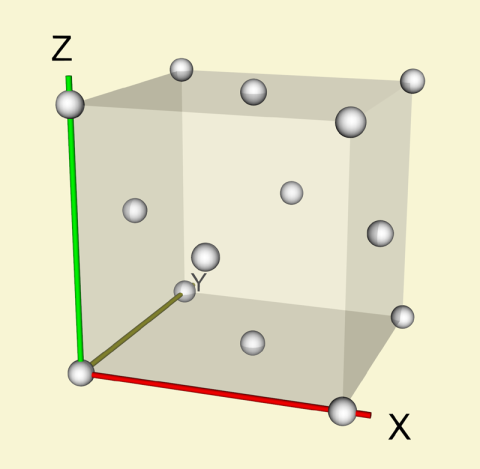
\includegraphics[width=0.4\textwidth]{fcc.png}
	\caption{A picture showing the fcc structure of the rare gas solids considered in this document.}
	\label{fig:fcc}
\end{figure}

\section{The Brillouin Zone and Symmetry Direction}
While its beyond this report to describe the Brillouin zone and its relation to the crystal structure in proper way, it is instructive to have a short note about it. Basically the $\mathbf{k}$ vectors in the ansatz made in equation \ref{eq:ansatz} are inside this zone. Thus we should have periodicy in the symmetry directions as we look at the frequencies. In figure \ref{fig:fccBrillouin} we can see this Brillouin zone for the crystal structure we are looking at. 
\begin{figure}[H]
	\centering
	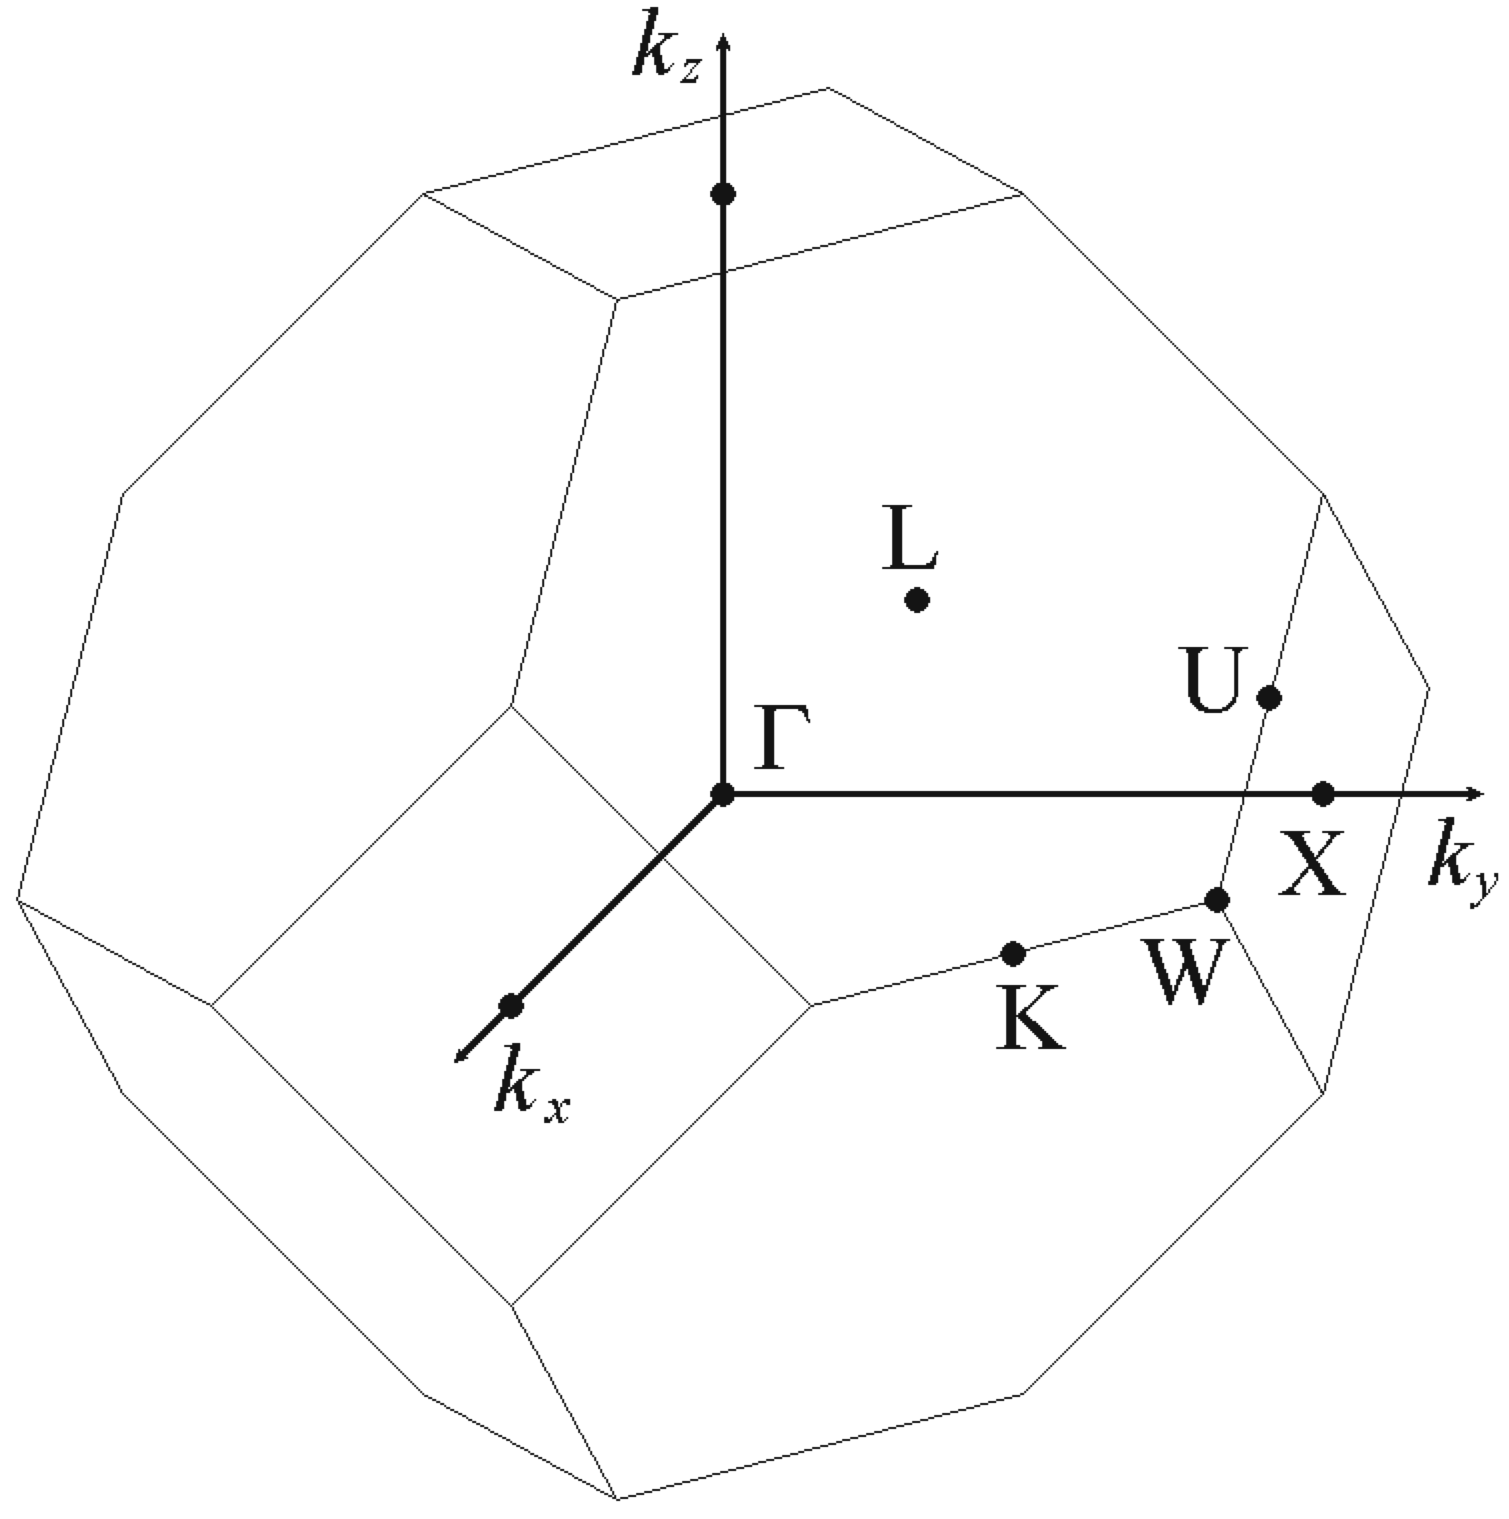
\includegraphics[width=0.4\textwidth]{fccBrillouin.png}
	\caption{A picture showing the first Brillouin zone for solids in the fcc structure. The symmetry directions are marked as $\mathbf{k}_x$,$\mathbf{k}_y$ and $\mathbf{k}_z$ }
	\label{fig:fccBrillouin}
\end{figure}

%%%%%%%%%%%%%%%%%%%%%%%%%%%%%%%%%%%%%%%%%%%%%%%%%%CODE
\section{Code}
In order to obtain usable values for the phonon frequencies, volume dependency of phonon frequencies and the heat capacity in the different rare gases using solid state physics theory, we have developed some code that calculate this numerically. Here we go through the code and its design.
\subsection{Algorithm design}
The code is written in $C$ and has been divided into two files: \verb+phonons.c+ and \verb+frequencies.c+. In \verb+frequencies.c+ we calculate the phonon frequencies possible in the rare gas solids we are looking at. This is done by solving the eigenvalue problem described by equation \ref{eq:omega} and \ref{eq:omegaRest}. The declaration of the frequencies function that does this calculation in this file is as follows
\begin{lstlisting}
 void frequencies(double A, double B, double m, double *q, 
				double *omega, double *eps);
\end{lstlisting}
where \verb+A+ and \verb+B+ are the constants described by equation \ref{eq:AB}, \verb+m+ is the mass of the atoms at the sites in the lattice, \verb+q+ are the modified k vector values, \verb+omega+ and \verb+eps+ are the return values where \verb+omega+ are the frequencies in the tree different directions and \verb+eps+ are the vector corresponding to each frequency describing its direction. This is a separate function since it is essential in not only calculating the frequency but the volume dependency of the frequency as well as the heat capacity of the rare gas solids. Its worth to also note that the eigenvalues \verb+omega+ and its corresponding eigenvector \verb+eps+ is sorted so by eigenvalue value in ascending order.

In \verb+phonons.c+ the rest of the program resides. Its main function is to use the frequency function to print usable data, calculate the volume dependency of the phonon frequencies as well as calculating heat capacity using solid state theory of the rare gas solids. In order to keep track of all the different rare gas properties a substance structure is declared in \verb+phonons.c+ as follows
\begin{lstlisting}
typedef struct sp{
	double sigma;
	double eps;
	double rnn;
	double m;
}sp;
\end{lstlisting}
where \verb+sigma+, \verb+eps+, \verb+rnn+ and \verb+m+ represents $\sigma$, $\epsilon$, $r$ and $m$ respectively from equation \ref{eq:pot}. The substance properties structure are then passed to different functions as a more collected argument. 

In order to use the \verb+frequencies+ function and write out different phonon frequencies that exists in a certain rare gas solid a function declared as 
\begin{lstlisting}
double* freqEval(sp sub, double* q)
\end{lstlisting} 
has been written. The inputs are simply a substance properties structure \verb+sub+ and a \verb+q+ vector, describing for which point the frequencies should be evaluated. The function returns an array with the three frequencies at the position described by \verb+q+. In order to calculate multiple frequencies evenly distributed between two \verb+q+ vectors a function declared as 
\begin{lstlisting}
void nEval(sp sub, double *q1, double *q2, int n, double* (*evalFunc)(sp, double*))
\end{lstlisting}
has been written. The inputs are the substance properties structure \verb+sub+, two \verb+q+ vectors \verb+q1+ and \verb+q2+, the number of \verb+n+ evenly spaced points to evaluate between \verb+q1+ and \verb+q2+ and a function pointer 
\verb+evalFunc+ that gets called at every point. If the frequencies is what is interesting the \verb+freqEval+ is the function passed as the last argument.


In order to calculate the volume dependency of the phonon frequencies a function declared as
\begin{lstlisting}
double* volDepEval(sp sub, double *q)
\end{lstlisting} 
has been written. The input are the substance properties structure \verb+sub+ and a vector \verb+q+ again describing the position we are interested in. The return value are the volume dependencies for the phonon frequencies. In order to calculate the volume dependency equation \ref{eq:volDep} has been used, then to estimate the derivate equation \ref{eq:derivate} is used. In order to calculate multiple frequencies evenly distributed between two \verb+q+ vectors we can use \verb+nEval+ again as done previously with \verb+freqEval+. The difference is that the last argument in \verb+nEval+ becomes \verb+volDepEval+.

If one instead are interested in the heat capacity for one of the gases the function declared as
\begin{lstlisting}
double cvEval(sp sub, double T)
\end{lstlisting} 
has been written. Here the input is only the substance properties structure \verb+sub+ and the temperature in Kelvin \verb+T+. The function returns the heat capacity. The heat capacity is calculated using equation \ref{eq:CV} and a some predefined values for \verb+q+ and the weights that holds for all gases that the program is implemented for. These 48 values are defined in the top of the program. Since this equation do not follow the same structure as \verb+freqEval+ and \verb+volDepEval+ a separate function to calculate multiple heat capacities between two temperatures has been written. This function is declared as
\begin{lstlisting}
void nCvEval(sp sub, double T1, double T2, int n)
\end{lstlisting}
where the input is the substance properties structure \verb+sub+, the two temperatures \verb+T1+ and \verb+T2+ which between the heat capacity shall be calculated in \verb+n+ points.  

Outside of that the code is responsible for user input/output. Making sure that the input is correctly interpreted and that the output follows a proper output formatting that was described in the program specification. This is mainly done via the nested switch statement in the \verb+main+ function and the \verb+printVal+ function.

\subsection{Typical Program Execution}
When the arguments are passed to the program at execution the proper substance structure is loaded and the calculation starts. Depending on what one are interested in, phonon frequencies, volume dependency of phonon frequencies or heat capacity of the gas, different functions are called in a nested switch statement in the main function. The code has been clearly divided for the different use cases so the structure should be very clear for a beginner who reads the code. There is also basic error checking made to make sure that the input is properly formatted.

An example command could be
\begin{lstlisting}
>phonons Xe cv 50 100
\end{lstlisting}
Then the program loads the substance structure related to \verb+Xe+ and the function \verb+nCvEval+ is be called so that it evaluate the heat capacity of a Xe-gas at ten points between 50 and 100 Kelvin spaced equally. \verb+nCvEval+ in turns call \verb+cvEval+ for every point that needs to be evaluated and \verb+cvEval+ calculate the heat capacity with help of the \verb+frequencies+ function and equation \ref{eq:CV} outputs
\begin{lstlisting}
50 678837
55 685602
60 690814
65 694912
70 698189
75 700850
80 703039
85 704861
90 706393
95 707694
\end{lstlisting}

\subsection{Solving the Eigenvalue Problem}
In order to solve the eigenvalue problem in the \verb+frequencies+ function we have used the GSL library. More specifically the function declared as
\begin{lstlisting}
int gsl_eigen_symmv (gsl_matrix * A, gsl_vector * eval, gsl_matrix * evec, gsl_eigen_symmv_workspace * w)
\end{lstlisting}
where the the input is the matrix \verb+A+ and the output \verb+eval+ and \verb+evec+ gives the eigenvalues and eigenvectors respectively. The last input in the function \verb+w+ is nothing more than some work space for the function to do its numerical scheme. The function uses the symmetric bidiagonalization and QR reduction method described in section 8.3 of \cite{bib:num}.

\subsection{Running the Code}
To run the code simply log into to sesam\footnote{A server for the institution for physics on UmU} and go into the directory
\begin{verbatim}
~jeve0010/Documents/jesper/fnm/lab2/src
\end{verbatim}
There the phonon code resides. By calling on \verb+make+ you can make sure that the code is up to date. Then simply execute the program \verb+./phonons+ with whatever command line arguments you want. Beyond that there exists code in the subdirectory \verb+plots/code+ which generate and plot data. The bash scripts \verb+makeFreqData.sh+,\verb+makeVolDepData.sh+ and \verb+makeCvData.sh+ generate the data, while the matlab scripts \verb+plotFreq.m+,\verb+plotVolDep.m+ and \verb+plotCv.m+ generate the plots used in this report. 

\newpage
\section{Results}
In this section we will go through different results specifically for the Argon solid, plots for the other gases exists in the appendix. Basically the same conclusions can be drawn from all the gases except small differences. Looking at figure \ref{fig:ArFreqResult} we can see the frequencies in the symmetry directions. Why the plot is not going on longer can clearly be seen in figure \ref{fig:ArFreqResultLonger}. The frequencies are basically periodic in the Brillouin zone. In figure \ref{fig:ArVolDepResult} we can see the volume dependency of the phonon frequencies in the Argon solid. Lastly we can see the heat capacity calculated for the Argon solid using both the numerically solved for solid state theory and using thermal physics theory in figure \ref{fig:ArCvResult}.
\iftikz
\begin{figure}[H]
	\centering
	\setlength\figureheight{4cm} 
	\setlength\figurewidth{15cm}
	% This file was created by matlab2tikz.
% Minimal pgfplots version: 1.3
%
%The latest updates can be retrieved from
%  http://www.mathworks.com/matlabcentral/fileexchange/22022-matlab2tikz
%where you can also make suggestions and rate matlab2tikz.
%
\definecolor{mycolor1}{rgb}{1.00000,0.00000,1.00000}%
%
\begin{tikzpicture}

\begin{axis}[%
width=0.261848\figurewidth,
height=\figureheight,
at={(0.344536\figurewidth,0\figureheight)},
scale only axis,
xmin=0,
xmax=200,
xtick={0,100,200},
xticklabels={{[000]},{[110]},{[220]}},
ymin=0,
ymax=12000000000000,
ylabel={$\omega(\mathbf{q})$ (rad/s)},
title style={font=\bfseries},
title={Ar Freq in [110]},
title style={font=\small},ticklabel style={font=\tiny}
]
\addplot [color=mycolor1,only marks,mark=x,mark options={solid},forget plot]
  table[row sep=crcr]{%
1	0\\
11	1261040000000\\
21	2486890000000\\
31	3644040000000\\
41	4702200000000\\
51	5635350000000\\
61	6422350000000\\
71	7047040000000\\
81	7497880000000\\
91	7767380000000\\
101	7851410000000\\
111	7748730000000\\
121	7460860000000\\
131	6992240000000\\
141	6350730000000\\
151	5548300000000\\
161	4601620000000\\
171	3532310000000\\
181	2366860000000\\
191	1135950000000\\
};
\addplot [color=mycolor1,solid,forget plot]
  table[row sep=crcr]{%
1	0\\
2	126691000000\\
3	253346000000\\
4	379929000000\\
5	506406000000\\
6	632741000000\\
7	758898000000\\
8	884842000000\\
9	1010540000000\\
10	1135950000000\\
11	1261040000000\\
12	1385780000000\\
13	1510130000000\\
14	1634060000000\\
15	1757530000000\\
16	1880520000000\\
17	2002970000000\\
18	2124870000000\\
19	2246180000000\\
20	2366860000000\\
21	2486890000000\\
22	2606220000000\\
23	2724840000000\\
24	2842700000000\\
25	2959780000000\\
26	3076040000000\\
27	3191450000000\\
28	3305990000000\\
29	3419620000000\\
30	3532310000000\\
31	3644040000000\\
32	3754780000000\\
33	3864490000000\\
34	3973160000000\\
35	4080750000000\\
36	4187230000000\\
37	4292590000000\\
38	4396790000000\\
39	4499810000000\\
40	4601620000000\\
41	4702200000000\\
42	4801530000000\\
43	4899580000000\\
44	4996330000000\\
45	5091760000000\\
46	5185840000000\\
47	5278560000000\\
48	5369890000000\\
49	5459810000000\\
50	5548300000000\\
51	5635350000000\\
52	5720930000000\\
53	5805030000000\\
54	5887630000000\\
55	5968700000000\\
56	6048240000000\\
57	6126230000000\\
58	6202650000000\\
59	6277490000000\\
60	6350730000000\\
61	6422350000000\\
62	6492350000000\\
63	6560710000000\\
64	6627410000000\\
65	6692450000000\\
66	6755810000000\\
67	6817480000000\\
68	6877450000000\\
69	6935700000000\\
70	6992240000000\\
71	7047040000000\\
72	7100100000000\\
73	7151410000000\\
74	7200960000000\\
75	7248740000000\\
76	7294750000000\\
77	7338970000000\\
78	7381400000000\\
79	7422030000000\\
80	7460860000000\\
81	7497880000000\\
82	7533090000000\\
83	7566470000000\\
84	7598020000000\\
85	7627740000000\\
86	7655630000000\\
87	7681680000000\\
88	7705880000000\\
89	7728230000000\\
90	7748730000000\\
91	7767380000000\\
92	7784170000000\\
93	7799100000000\\
94	7812170000000\\
95	7823380000000\\
96	7832720000000\\
97	7840190000000\\
98	7845800000000\\
99	7849540000000\\
100	7851410000000\\
101	7851410000000\\
102	7849540000000\\
103	7845800000000\\
104	7840190000000\\
105	7832720000000\\
106	7823380000000\\
107	7812170000000\\
108	7799100000000\\
109	7784170000000\\
110	7767380000000\\
111	7748730000000\\
112	7728230000000\\
113	7705880000000\\
114	7681680000000\\
115	7655630000000\\
116	7627740000000\\
117	7598020000000\\
118	7566470000000\\
119	7533090000000\\
120	7497880000000\\
121	7460860000000\\
122	7422030000000\\
123	7381400000000\\
124	7338970000000\\
125	7294750000000\\
126	7248740000000\\
127	7200960000000\\
128	7151410000000\\
129	7100100000000\\
130	7047040000000\\
131	6992240000000\\
132	6935700000000\\
133	6877450000000\\
134	6817480000000\\
135	6755810000000\\
136	6692450000000\\
137	6627410000000\\
138	6560710000000\\
139	6492350000000\\
140	6422350000000\\
141	6350730000000\\
142	6277490000000\\
143	6202650000000\\
144	6126230000000\\
145	6048240000000\\
146	5968700000000\\
147	5887630000000\\
148	5805030000000\\
149	5720930000000\\
150	5635350000000\\
151	5548300000000\\
152	5459810000000\\
153	5369890000000\\
154	5278560000000\\
155	5185840000000\\
156	5091760000000\\
157	4996330000000\\
158	4899580000000\\
159	4801530000000\\
160	4702200000000\\
161	4601620000000\\
162	4499810000000\\
163	4396790000000\\
164	4292590000000\\
165	4187230000000\\
166	4080750000000\\
167	3973160000000\\
168	3864490000000\\
169	3754780000000\\
170	3644040000000\\
171	3532310000000\\
172	3419620000000\\
173	3305990000000\\
174	3191450000000\\
175	3076040000000\\
176	2959780000000\\
177	2842700000000\\
178	2724840000000\\
179	2606220000000\\
180	2486890000000\\
181	2366860000000\\
182	2246180000000\\
183	2124870000000\\
184	2002970000000\\
185	1880520000000\\
186	1757530000000\\
187	1634060000000\\
188	1510130000000\\
189	1385780000000\\
190	1261040000000\\
191	1135950000000\\
192	1010540000000\\
193	884842000000\\
194	758898000000\\
195	632741000000\\
196	506406000000\\
197	379929000000\\
198	253346000000\\
199	126691000000\\
200	0\\
};
\addplot [color=orange,solid,forget plot]
  table[row sep=crcr]{%
1	0\\
2	175288000000\\
3	350530000000\\
4	525678000000\\
5	700687000000\\
6	875509000000\\
7	1050100000000\\
8	1224410000000\\
9	1398400000000\\
10	1572010000000\\
11	1745210000000\\
12	1917940000000\\
13	2090160000000\\
14	2261830000000\\
15	2432900000000\\
16	2603330000000\\
17	2773070000000\\
18	2942070000000\\
19	3110300000000\\
20	3277700000000\\
21	3444240000000\\
22	3609870000000\\
23	3774540000000\\
24	3938230000000\\
25	4100880000000\\
26	4262440000000\\
27	4422890000000\\
28	4582180000000\\
29	4740270000000\\
30	4897110000000\\
31	5052670000000\\
32	5206920000000\\
33	5359800000000\\
34	5511290000000\\
35	5661340000000\\
36	5809910000000\\
37	5956980000000\\
38	6102500000000\\
39	6246440000000\\
40	6388760000000\\
41	6529430000000\\
42	6668410000000\\
43	6805670000000\\
44	6941180000000\\
45	7074900000000\\
46	7206810000000\\
47	7336860000000\\
48	7465040000000\\
49	7591310000000\\
50	7715630000000\\
51	7837990000000\\
52	7958350000000\\
53	8076690000000\\
54	8192970000000\\
55	8307180000000\\
56	8419280000000\\
57	8529250000000\\
58	8637060000000\\
59	8742700000000\\
60	8846130000000\\
61	8947330000000\\
62	9046290000000\\
63	9142980000000\\
64	9237370000000\\
65	9329460000000\\
66	9419210000000\\
67	9506610000000\\
68	9506830000000\\
69	9461000000000\\
70	9411490000000\\
71	9358580000000\\
72	9302550000000\\
73	9243680000000\\
74	9182290000000\\
75	9118690000000\\
76	9053210000000\\
77	8986190000000\\
78	8917970000000\\
79	8848910000000\\
80	8779380000000\\
81	8709740000000\\
82	8640380000000\\
83	8571670000000\\
84	8504010000000\\
85	8437780000000\\
86	8373360000000\\
87	8311140000000\\
88	8251480000000\\
89	8194770000000\\
90	8141350000000\\
91	8091570000000\\
92	8045750000000\\
93	8004190000000\\
94	7967170000000\\
95	7934940000000\\
96	7907740000000\\
97	7885740000000\\
98	7869100000000\\
99	7857940000000\\
100	7852340000000\\
101	7852340000000\\
102	7857940000000\\
103	7869100000000\\
104	7885740000000\\
105	7907740000000\\
106	7934940000000\\
107	7967170000000\\
108	8004190000000\\
109	8045750000000\\
110	8091570000000\\
111	8141350000000\\
112	8194770000000\\
113	8251480000000\\
114	8311140000000\\
115	8373360000000\\
116	8437780000000\\
117	8504010000000\\
118	8571670000000\\
119	8640380000000\\
120	8709740000000\\
121	8779380000000\\
122	8848910000000\\
123	8917970000000\\
124	8986190000000\\
125	9053210000000\\
126	9118690000000\\
127	9182290000000\\
128	9243680000000\\
129	9302550000000\\
130	9358580000000\\
131	9411490000000\\
132	9461000000000\\
133	9506830000000\\
134	9506610000000\\
135	9419210000000\\
136	9329460000000\\
137	9237370000000\\
138	9142980000000\\
139	9046290000000\\
140	8947330000000\\
141	8846130000000\\
142	8742700000000\\
143	8637060000000\\
144	8529250000000\\
145	8419280000000\\
146	8307180000000\\
147	8192970000000\\
148	8076690000000\\
149	7958350000000\\
150	7837990000000\\
151	7715630000000\\
152	7591310000000\\
153	7465040000000\\
154	7336860000000\\
155	7206810000000\\
156	7074900000000\\
157	6941180000000\\
158	6805670000000\\
159	6668410000000\\
160	6529430000000\\
161	6388760000000\\
162	6246440000000\\
163	6102500000000\\
164	5956980000000\\
165	5809910000000\\
166	5661340000000\\
167	5511290000000\\
168	5359800000000\\
169	5206920000000\\
170	5052670000000\\
171	4897110000000\\
172	4740270000000\\
173	4582180000000\\
174	4422890000000\\
175	4262440000000\\
176	4100880000000\\
177	3938230000000\\
178	3774540000000\\
179	3609870000000\\
180	3444240000000\\
181	3277700000000\\
182	3110300000000\\
183	2942070000000\\
184	2773070000000\\
185	2603330000000\\
186	2432900000000\\
187	2261830000000\\
188	2090160000000\\
189	1917940000000\\
190	1745210000000\\
191	1572010000000\\
192	1398400000000\\
193	1224410000000\\
194	1050100000000\\
195	875509000000\\
196	700687000000\\
197	525678000000\\
198	350530000000\\
199	175288000000\\
200	0\\
};
\addplot [color=black,solid,forget plot]
  table[row sep=crcr]{%
1	0\\
2	273382000000\\
3	546534000000\\
4	819224000000\\
5	1091220000000\\
6	1362310000000\\
7	1632240000000\\
8	1900800000000\\
9	2167760000000\\
10	2432900000000\\
11	2696000000000\\
12	2956830000000\\
13	3215180000000\\
14	3470850000000\\
15	3723610000000\\
16	3973260000000\\
17	4219600000000\\
18	4462430000000\\
19	4701550000000\\
20	4936770000000\\
21	5167910000000\\
22	5394780000000\\
23	5617200000000\\
24	5835010000000\\
25	6048030000000\\
26	6256110000000\\
27	6459090000000\\
28	6656830000000\\
29	6849170000000\\
30	7035990000000\\
31	7217150000000\\
32	7392530000000\\
33	7562030000000\\
34	7725510000000\\
35	7882900000000\\
36	8034090000000\\
37	8179010000000\\
38	8317560000000\\
39	8449690000000\\
40	8575320000000\\
41	8694420000000\\
42	8806940000000\\
43	8912840000000\\
44	9012090000000\\
45	9104680000000\\
46	9190610000000\\
47	9269870000000\\
48	9342480000000\\
49	9408450000000\\
50	9467820000000\\
51	9520640000000\\
52	9566940000000\\
53	9606800000000\\
54	9640290000000\\
55	9667490000000\\
56	9688490000000\\
57	9703410000000\\
58	9712350000000\\
59	9715440000000\\
60	9712820000000\\
61	9704640000000\\
62	9691070000000\\
63	9672270000000\\
64	9648440000000\\
65	9619760000000\\
66	9586450000000\\
67	9548730000000\\
68	9591630000000\\
69	9674270000000\\
70	9754510000000\\
71	9832320000000\\
72	9907690000000\\
73	9980600000000\\
74	10051000000000\\
75	10119000000000\\
76	10184500000000\\
77	10247400000000\\
78	10307800000000\\
79	10365700000000\\
80	10421000000000\\
81	10473800000000\\
82	10524000000000\\
83	10571600000000\\
84	10616600000000\\
85	10659000000000\\
86	10698900000000\\
87	10736000000000\\
88	10770600000000\\
89	10802500000000\\
90	10831800000000\\
91	10858500000000\\
92	10882500000000\\
93	10903800000000\\
94	10922500000000\\
95	10938500000000\\
96	10951900000000\\
97	10962600000000\\
98	10970600000000\\
99	10975900000000\\
100	10978600000000\\
101	10978600000000\\
102	10975900000000\\
103	10970600000000\\
104	10962600000000\\
105	10951900000000\\
106	10938500000000\\
107	10922500000000\\
108	10903800000000\\
109	10882500000000\\
110	10858500000000\\
111	10831800000000\\
112	10802500000000\\
113	10770600000000\\
114	10736000000000\\
115	10698900000000\\
116	10659000000000\\
117	10616600000000\\
118	10571600000000\\
119	10524000000000\\
120	10473800000000\\
121	10421000000000\\
122	10365700000000\\
123	10307800000000\\
124	10247400000000\\
125	10184500000000\\
126	10119000000000\\
127	10051000000000\\
128	9980600000000\\
129	9907690000000\\
130	9832320000000\\
131	9754510000000\\
132	9674270000000\\
133	9591630000000\\
134	9548730000000\\
135	9586450000000\\
136	9619760000000\\
137	9648440000000\\
138	9672270000000\\
139	9691070000000\\
140	9704640000000\\
141	9712820000000\\
142	9715440000000\\
143	9712350000000\\
144	9703410000000\\
145	9688490000000\\
146	9667490000000\\
147	9640290000000\\
148	9606800000000\\
149	9566940000000\\
150	9520640000000\\
151	9467820000000\\
152	9408450000000\\
153	9342480000000\\
154	9269870000000\\
155	9190610000000\\
156	9104680000000\\
157	9012090000000\\
158	8912840000000\\
159	8806940000000\\
160	8694420000000\\
161	8575320000000\\
162	8449690000000\\
163	8317560000000\\
164	8179010000000\\
165	8034090000000\\
166	7882900000000\\
167	7725510000000\\
168	7562030000000\\
169	7392530000000\\
170	7217150000000\\
171	7035990000000\\
172	6849170000000\\
173	6656830000000\\
174	6459090000000\\
175	6256110000000\\
176	6048030000000\\
177	5835010000000\\
178	5617200000000\\
179	5394780000000\\
180	5167910000000\\
181	4936770000000\\
182	4701550000000\\
183	4462430000000\\
184	4219600000000\\
185	3973260000000\\
186	3723610000000\\
187	3470850000000\\
188	3215180000000\\
189	2956830000000\\
190	2696000000000\\
191	2432900000000\\
192	2167760000000\\
193	1900800000000\\
194	1632240000000\\
195	1362310000000\\
196	1091220000000\\
197	819224000000\\
198	546534000000\\
199	273382000000\\
200	0.00132906\\
};
\end{axis}

\begin{axis}[%
width=0.261848\figurewidth,
height=\figureheight,
at={(0.689073\figurewidth,0\figureheight)},
scale only axis,
xmin=0,
xmax=200,
xtick={0,100,200},
xticklabels={{[000]},{[111]},{[222]}},
ymin=0,
ymax=12000000000000,
ylabel={$\omega(\mathbf{q})$ (rad/s)},
title style={font=\bfseries},
title={Ar Freq in [111]},
title style={font=\small},ticklabel style={font=\tiny}
]
\addplot [color=mycolor1,only marks,mark=x,mark options={solid},forget plot]
  table[row sep=crcr]{%
1	0\\
11	1743160000000\\
21	3313990000000\\
31	4557180000000\\
41	5349820000000\\
51	5613550000000\\
61	5322300000000\\
71	4504860000000\\
81	3242050000000\\
91	1658710000000\\
101	88619700000\\
111	1827190000000\\
121	3385110000000\\
131	4608360000000\\
141	5376010000000\\
151	5612150000000\\
161	5293460000000\\
171	4451420000000\\
181	3169300000000\\
191	1573840000000\\
};
\addplot [color=mycolor1,solid,forget plot]
  table[row sep=crcr]{%
1	0\\
2	177217000000\\
3	354258000000\\
4	530945000000\\
5	707103000000\\
6	882557000000\\
7	1057130000000\\
8	1230650000000\\
9	1402940000000\\
10	1573840000000\\
11	1743160000000\\
12	1910750000000\\
13	2076440000000\\
14	2240050000000\\
15	2401430000000\\
16	2560420000000\\
17	2716850000000\\
18	2870580000000\\
19	3021440000000\\
20	3169300000000\\
21	3313990000000\\
22	3455380000000\\
23	3593330000000\\
24	3727690000000\\
25	3858340000000\\
26	3985140000000\\
27	4107970000000\\
28	4226700000000\\
29	4341230000000\\
30	4451420000000\\
31	4557180000000\\
32	4658390000000\\
33	4754960000000\\
34	4846790000000\\
35	4933790000000\\
36	5015870000000\\
37	5092950000000\\
38	5164960000000\\
39	5231810000000\\
40	5293460000000\\
41	5349820000000\\
42	5400850000000\\
43	5446500000000\\
44	5486720000000\\
45	5521470000000\\
46	5550710000000\\
47	5574420000000\\
48	5592580000000\\
49	5605160000000\\
50	5612150000000\\
51	5613550000000\\
52	5609360000000\\
53	5599570000000\\
54	5584200000000\\
55	5563260000000\\
56	5536780000000\\
57	5504780000000\\
58	5467290000000\\
59	5424350000000\\
60	5376010000000\\
61	5322300000000\\
62	5263290000000\\
63	5199030000000\\
64	5129600000000\\
65	5055040000000\\
66	4975450000000\\
67	4890900000000\\
68	4801480000000\\
69	4707260000000\\
70	4608360000000\\
71	4504860000000\\
72	4396870000000\\
73	4284500000000\\
74	4167860000000\\
75	4047060000000\\
76	3922230000000\\
77	3793490000000\\
78	3660960000000\\
79	3524790000000\\
80	3385110000000\\
81	3242050000000\\
82	3095750000000\\
83	2946380000000\\
84	2794060000000\\
85	2638960000000\\
86	2481230000000\\
87	2321030000000\\
88	2158510000000\\
89	1993840000000\\
90	1827190000000\\
91	1658710000000\\
92	1488580000000\\
93	1316960000000\\
94	1144030000000\\
95	969964000000\\
96	794929000000\\
97	619101000000\\
98	442657000000\\
99	265771000000\\
100	88619700000\\
101	88619700000\\
102	265771000000\\
103	442657000000\\
104	619101000000\\
105	794929000000\\
106	969964000000\\
107	1144030000000\\
108	1316960000000\\
109	1488580000000\\
110	1658710000000\\
111	1827190000000\\
112	1993840000000\\
113	2158510000000\\
114	2321030000000\\
115	2481230000000\\
116	2638960000000\\
117	2794060000000\\
118	2946380000000\\
119	3095750000000\\
120	3242050000000\\
121	3385110000000\\
122	3524790000000\\
123	3660960000000\\
124	3793490000000\\
125	3922230000000\\
126	4047060000000\\
127	4167860000000\\
128	4284500000000\\
129	4396870000000\\
130	4504860000000\\
131	4608360000000\\
132	4707260000000\\
133	4801480000000\\
134	4890900000000\\
135	4975450000000\\
136	5055040000000\\
137	5129600000000\\
138	5199030000000\\
139	5263290000000\\
140	5322300000000\\
141	5376010000000\\
142	5424350000000\\
143	5467290000000\\
144	5504780000000\\
145	5536780000000\\
146	5563260000000\\
147	5584200000000\\
148	5599570000000\\
149	5609360000000\\
150	5613550000000\\
151	5612150000000\\
152	5605160000000\\
153	5592580000000\\
154	5574420000000\\
155	5550710000000\\
156	5521470000000\\
157	5486720000000\\
158	5446500000000\\
159	5400850000000\\
160	5349820000000\\
161	5293460000000\\
162	5231810000000\\
163	5164960000000\\
164	5092950000000\\
165	5015870000000\\
166	4933790000000\\
167	4846790000000\\
168	4754960000000\\
169	4658390000000\\
170	4557180000000\\
171	4451420000000\\
172	4341230000000\\
173	4226700000000\\
174	4107970000000\\
175	3985140000000\\
176	3858340000000\\
177	3727690000000\\
178	3593330000000\\
179	3455380000000\\
180	3313990000000\\
181	3169300000000\\
182	3021440000000\\
183	2870580000000\\
184	2716850000000\\
185	2560420000000\\
186	2401430000000\\
187	2240050000000\\
188	2076440000000\\
189	1910750000000\\
190	1743160000000\\
191	1573840000000\\
192	1402940000000\\
193	1230650000000\\
194	1057130000000\\
195	882557000000\\
196	707103000000\\
197	530945000000\\
198	354258000000\\
199	177217000000\\
200	0\\
};
\addplot [color=orange,solid,forget plot]
  table[row sep=crcr]{%
1	0\\
2	177217000000\\
3	354258000000\\
4	530945000000\\
5	707103000000\\
6	882557000000\\
7	1057130000000\\
8	1230650000000\\
9	1402940000000\\
10	1573840000000\\
11	1743160000000\\
12	1910750000000\\
13	2076440000000\\
14	2240050000000\\
15	2401430000000\\
16	2560420000000\\
17	2716850000000\\
18	2870580000000\\
19	3021440000000\\
20	3169300000000\\
21	3313990000000\\
22	3455380000000\\
23	3593330000000\\
24	3727690000000\\
25	3858340000000\\
26	3985140000000\\
27	4107970000000\\
28	4226700000000\\
29	4341230000000\\
30	4451420000000\\
31	4557180000000\\
32	4658390000000\\
33	4754960000000\\
34	4846790000000\\
35	4933790000000\\
36	5015870000000\\
37	5092950000000\\
38	5164960000000\\
39	5231810000000\\
40	5293460000000\\
41	5349820000000\\
42	5400850000000\\
43	5446500000000\\
44	5486720000000\\
45	5521470000000\\
46	5550710000000\\
47	5574420000000\\
48	5592580000000\\
49	5605160000000\\
50	5612150000000\\
51	5613550000000\\
52	5609360000000\\
53	5599570000000\\
54	5584200000000\\
55	5563260000000\\
56	5536780000000\\
57	5504780000000\\
58	5467290000000\\
59	5424350000000\\
60	5376010000000\\
61	5322300000000\\
62	5263290000000\\
63	5199030000000\\
64	5129600000000\\
65	5055040000000\\
66	4975450000000\\
67	4890900000000\\
68	4801480000000\\
69	4707260000000\\
70	4608360000000\\
71	4504860000000\\
72	4396870000000\\
73	4284500000000\\
74	4167860000000\\
75	4047060000000\\
76	3922230000000\\
77	3793490000000\\
78	3660960000000\\
79	3524790000000\\
80	3385110000000\\
81	3242050000000\\
82	3095750000000\\
83	2946380000000\\
84	2794060000000\\
85	2638960000000\\
86	2481230000000\\
87	2321030000000\\
88	2158510000000\\
89	1993840000000\\
90	1827190000000\\
91	1658710000000\\
92	1488580000000\\
93	1316960000000\\
94	1144030000000\\
95	969964000000\\
96	794929000000\\
97	619101000000\\
98	442657000000\\
99	265771000000\\
100	88619700000\\
101	88619700000\\
102	265771000000\\
103	442657000000\\
104	619101000000\\
105	794929000000\\
106	969964000000\\
107	1144030000000\\
108	1316960000000\\
109	1488580000000\\
110	1658710000000\\
111	1827190000000\\
112	1993840000000\\
113	2158510000000\\
114	2321030000000\\
115	2481230000000\\
116	2638960000000\\
117	2794060000000\\
118	2946380000000\\
119	3095750000000\\
120	3242050000000\\
121	3385110000000\\
122	3524790000000\\
123	3660960000000\\
124	3793490000000\\
125	3922230000000\\
126	4047060000000\\
127	4167860000000\\
128	4284500000000\\
129	4396870000000\\
130	4504860000000\\
131	4608360000000\\
132	4707260000000\\
133	4801480000000\\
134	4890900000000\\
135	4975450000000\\
136	5055040000000\\
137	5129600000000\\
138	5199030000000\\
139	5263290000000\\
140	5322300000000\\
141	5376010000000\\
142	5424350000000\\
143	5467290000000\\
144	5504780000000\\
145	5536780000000\\
146	5563260000000\\
147	5584200000000\\
148	5599570000000\\
149	5609360000000\\
150	5613550000000\\
151	5612150000000\\
152	5605160000000\\
153	5592580000000\\
154	5574420000000\\
155	5550710000000\\
156	5521470000000\\
157	5486720000000\\
158	5446500000000\\
159	5400850000000\\
160	5349820000000\\
161	5293460000000\\
162	5231810000000\\
163	5164960000000\\
164	5092950000000\\
165	5015870000000\\
166	4933790000000\\
167	4846790000000\\
168	4754960000000\\
169	4658390000000\\
170	4557180000000\\
171	4451420000000\\
172	4341230000000\\
173	4226700000000\\
174	4107970000000\\
175	3985140000000\\
176	3858340000000\\
177	3727690000000\\
178	3593330000000\\
179	3455380000000\\
180	3313990000000\\
181	3169300000000\\
182	3021440000000\\
183	2870580000000\\
184	2716850000000\\
185	2560420000000\\
186	2401430000000\\
187	2240050000000\\
188	2076440000000\\
189	1910750000000\\
190	1743160000000\\
191	1573840000000\\
192	1402940000000\\
193	1230650000000\\
194	1057130000000\\
195	882557000000\\
196	707103000000\\
197	530945000000\\
198	354258000000\\
199	177217000000\\
200	0\\
};
\addplot [color=black,solid,forget plot]
  table[row sep=crcr]{%
1	0\\
2	345596000000\\
3	690848000000\\
4	1035410000000\\
5	1378940000000\\
6	1721100000000\\
7	2061540000000\\
8	2399930000000\\
9	2735920000000\\
10	3069180000000\\
11	3399390000000\\
12	3726210000000\\
13	4049310000000\\
14	4368380000000\\
15	4683090000000\\
16	4993140000000\\
17	5298210000000\\
18	5597990000000\\
19	5892200000000\\
20	6180530000000\\
21	6462700000000\\
22	6738430000000\\
23	7007440000000\\
24	7269470000000\\
25	7524250000000\\
26	7771530000000\\
27	8011070000000\\
28	8242610000000\\
29	8465950000000\\
30	8680840000000\\
31	8887080000000\\
32	9084460000000\\
33	9272780000000\\
34	9451870000000\\
35	9621520000000\\
36	9781590000000\\
37	9931910000000\\
38	10072300000000\\
39	10202700000000\\
40	10322900000000\\
41	10432800000000\\
42	10532400000000\\
43	10621400000000\\
44	10699800000000\\
45	10767600000000\\
46	10824600000000\\
47	10870800000000\\
48	10906200000000\\
49	10930800000000\\
50	10944400000000\\
51	10947100000000\\
52	10939000000000\\
53	10919900000000\\
54	10889900000000\\
55	10849100000000\\
56	10797400000000\\
57	10735000000000\\
58	10661900000000\\
59	10578200000000\\
60	10483900000000\\
61	10379200000000\\
62	10264100000000\\
63	10138800000000\\
64	10003400000000\\
65	9857980000000\\
66	9702770000000\\
67	9537880000000\\
68	9363490000000\\
69	9179760000000\\
70	8986890000000\\
71	8785050000000\\
72	8574460000000\\
73	8355320000000\\
74	8127850000000\\
75	7892280000000\\
76	7648850000000\\
77	7397780000000\\
78	7139350000000\\
79	6873790000000\\
80	6601390000000\\
81	6322400000000\\
82	6037120000000\\
83	5745810000000\\
84	5448780000000\\
85	5146310000000\\
86	4838720000000\\
87	4526300000000\\
88	4209370000000\\
89	3888250000000\\
90	3563240000000\\
91	3234690000000\\
92	2902910000000\\
93	2568240000000\\
94	2231010000000\\
95	1891550000000\\
96	1550210000000\\
97	1207330000000\\
98	863237000000\\
99	518287000000\\
100	172820000000\\
101	172820000000\\
102	518287000000\\
103	863237000000\\
104	1207330000000\\
105	1550210000000\\
106	1891550000000\\
107	2231010000000\\
108	2568240000000\\
109	2902910000000\\
110	3234690000000\\
111	3563240000000\\
112	3888250000000\\
113	4209370000000\\
114	4526300000000\\
115	4838720000000\\
116	5146310000000\\
117	5448780000000\\
118	5745810000000\\
119	6037120000000\\
120	6322400000000\\
121	6601390000000\\
122	6873790000000\\
123	7139350000000\\
124	7397780000000\\
125	7648850000000\\
126	7892280000000\\
127	8127850000000\\
128	8355320000000\\
129	8574460000000\\
130	8785050000000\\
131	8986890000000\\
132	9179760000000\\
133	9363490000000\\
134	9537880000000\\
135	9702770000000\\
136	9857980000000\\
137	10003400000000\\
138	10138800000000\\
139	10264100000000\\
140	10379200000000\\
141	10483900000000\\
142	10578200000000\\
143	10661900000000\\
144	10735000000000\\
145	10797400000000\\
146	10849100000000\\
147	10889900000000\\
148	10919900000000\\
149	10939000000000\\
150	10947100000000\\
151	10944400000000\\
152	10930800000000\\
153	10906200000000\\
154	10870800000000\\
155	10824600000000\\
156	10767600000000\\
157	10699800000000\\
158	10621400000000\\
159	10532400000000\\
160	10432800000000\\
161	10322900000000\\
162	10202700000000\\
163	10072300000000\\
164	9931910000000\\
165	9781590000000\\
166	9621520000000\\
167	9451870000000\\
168	9272780000000\\
169	9084460000000\\
170	8887080000000\\
171	8680840000000\\
172	8465950000000\\
173	8242610000000\\
174	8011070000000\\
175	7771530000000\\
176	7524250000000\\
177	7269470000000\\
178	7007440000000\\
179	6738430000000\\
180	6462700000000\\
181	6180530000000\\
182	5892200000000\\
183	5597990000000\\
184	5298210000000\\
185	4993140000000\\
186	4683090000000\\
187	4368380000000\\
188	4049310000000\\
189	3726210000000\\
190	3399390000000\\
191	3069180000000\\
192	2735920000000\\
193	2399930000000\\
194	2061540000000\\
195	1721100000000\\
196	1378940000000\\
197	1035410000000\\
198	690848000000\\
199	345596000000\\
200	0.00187957\\
};
\end{axis}

\begin{axis}[%
width=0.261848\figurewidth,
height=\figureheight,
at={(0\figurewidth,0\figureheight)},
scale only axis,
xmin=0,
xmax=200,
xtick={0,100,200},
xticklabels={{[000]},{[100]},{[200]}},
ymin=0,
ymax=12000000000000,
ylabel={$\omega(\mathbf{q})$ (rad/s)},
title style={font=\bfseries},
title={Ar Freq in [100]},
title style={font=\small},ticklabel style={font=\tiny}
]
\addplot [color=mycolor1,only marks,mark=x,mark options={solid},forget plot]
  table[row sep=crcr]{%
1	0\\
11	1234390000000\\
21	2438080000000\\
31	3581130000000\\
41	4635110000000\\
51	5573820000000\\
61	6373900000000\\
71	7015450000000\\
81	7482530000000\\
91	7763500000000\\
101	7851390000000\\
111	7744020000000\\
121	7444040000000\\
131	6958920000000\\
141	6300720000000\\
151	5485820000000\\
161	4534490000000\\
171	3470380000000\\
181	2319950000000\\
191	1111830000000\\
};
\addplot [color=mycolor1,solid,forget plot]
  table[row sep=crcr]{%
1	0\\
2	123948000000\\
3	247865000000\\
4	371720000000\\
5	495483000000\\
6	619122000000\\
7	742607000000\\
8	865906000000\\
9	988990000000\\
10	1111830000000\\
11	1234390000000\\
12	1356640000000\\
13	1478560000000\\
14	1600100000000\\
15	1721250000000\\
16	1841970000000\\
17	1962230000000\\
18	2082000000000\\
19	2201250000000\\
20	2319950000000\\
21	2438080000000\\
22	2555590000000\\
23	2672470000000\\
24	2788690000000\\
25	2904210000000\\
26	3019000000000\\
27	3133040000000\\
28	3246310000000\\
29	3358760000000\\
30	3470380000000\\
31	3581130000000\\
32	3690980000000\\
33	3799920000000\\
34	3907920000000\\
35	4014930000000\\
36	4120950000000\\
37	4225940000000\\
38	4329880000000\\
39	4432730000000\\
40	4534490000000\\
41	4635110000000\\
42	4734580000000\\
43	4832870000000\\
44	4929950000000\\
45	5025800000000\\
46	5120410000000\\
47	5213730000000\\
48	5305760000000\\
49	5396460000000\\
50	5485820000000\\
51	5573820000000\\
52	5660420000000\\
53	5745610000000\\
54	5829370000000\\
55	5911680000000\\
56	5992520000000\\
57	6071860000000\\
58	6149680000000\\
59	6225980000000\\
60	6300720000000\\
61	6373900000000\\
62	6445480000000\\
63	6515460000000\\
64	6583810000000\\
65	6650530000000\\
66	6715580000000\\
67	6778970000000\\
68	6840660000000\\
69	6900650000000\\
70	6958920000000\\
71	7015450000000\\
72	7070240000000\\
73	7123260000000\\
74	7174510000000\\
75	7223970000000\\
76	7271630000000\\
77	7317480000000\\
78	7361500000000\\
79	7403690000000\\
80	7444040000000\\
81	7482530000000\\
82	7519150000000\\
83	7553900000000\\
84	7586770000000\\
85	7617750000000\\
86	7646820000000\\
87	7674000000000\\
88	7699260000000\\
89	7722600000000\\
90	7744020000000\\
91	7763500000000\\
92	7781050000000\\
93	7796670000000\\
94	7810340000000\\
95	7822060000000\\
96	7831830000000\\
97	7839660000000\\
98	7845530000000\\
99	7849440000000\\
100	7851390000000\\
101	7851390000000\\
102	7849440000000\\
103	7845530000000\\
104	7839660000000\\
105	7831830000000\\
106	7822060000000\\
107	7810340000000\\
108	7796670000000\\
109	7781050000000\\
110	7763500000000\\
111	7744020000000\\
112	7722600000000\\
113	7699260000000\\
114	7674000000000\\
115	7646820000000\\
116	7617750000000\\
117	7586770000000\\
118	7553900000000\\
119	7519150000000\\
120	7482530000000\\
121	7444040000000\\
122	7403690000000\\
123	7361500000000\\
124	7317480000000\\
125	7271630000000\\
126	7223970000000\\
127	7174510000000\\
128	7123260000000\\
129	7070240000000\\
130	7015450000000\\
131	6958920000000\\
132	6900650000000\\
133	6840660000000\\
134	6778970000000\\
135	6715580000000\\
136	6650530000000\\
137	6583810000000\\
138	6515460000000\\
139	6445480000000\\
140	6373900000000\\
141	6300720000000\\
142	6225980000000\\
143	6149680000000\\
144	6071860000000\\
145	5992520000000\\
146	5911680000000\\
147	5829370000000\\
148	5745610000000\\
149	5660420000000\\
150	5573820000000\\
151	5485820000000\\
152	5396460000000\\
153	5305760000000\\
154	5213730000000\\
155	5120410000000\\
156	5025800000000\\
157	4929950000000\\
158	4832870000000\\
159	4734580000000\\
160	4635110000000\\
161	4534490000000\\
162	4432730000000\\
163	4329880000000\\
164	4225940000000\\
165	4120950000000\\
166	4014930000000\\
167	3907920000000\\
168	3799920000000\\
169	3690980000000\\
170	3581130000000\\
171	3470380000000\\
172	3358760000000\\
173	3246310000000\\
174	3133040000000\\
175	3019000000000\\
176	2904210000000\\
177	2788690000000\\
178	2672470000000\\
179	2555590000000\\
180	2438080000000\\
181	2319950000000\\
182	2201250000000\\
183	2082000000000\\
184	1962230000000\\
185	1841970000000\\
186	1721250000000\\
187	1600100000000\\
188	1478560000000\\
189	1356640000000\\
190	1234390000000\\
191	1111830000000\\
192	988990000000\\
193	865906000000\\
194	742607000000\\
195	619122000000\\
196	495483000000\\
197	371720000000\\
198	247865000000\\
199	123948000000\\
200	0\\
};
\addplot [color=orange,solid,forget plot]
  table[row sep=crcr]{%
1	0\\
2	123948000000\\
3	247865000000\\
4	371720000000\\
5	495483000000\\
6	619122000000\\
7	742607000000\\
8	865906000000\\
9	988990000000\\
10	1111830000000\\
11	1234390000000\\
12	1356640000000\\
13	1478560000000\\
14	1600100000000\\
15	1721250000000\\
16	1841970000000\\
17	1962230000000\\
18	2082000000000\\
19	2201250000000\\
20	2319950000000\\
21	2438080000000\\
22	2555590000000\\
23	2672470000000\\
24	2788690000000\\
25	2904210000000\\
26	3019000000000\\
27	3133040000000\\
28	3246310000000\\
29	3358760000000\\
30	3470380000000\\
31	3581130000000\\
32	3690980000000\\
33	3799920000000\\
34	3907920000000\\
35	4014930000000\\
36	4120950000000\\
37	4225940000000\\
38	4329880000000\\
39	4432730000000\\
40	4534490000000\\
41	4635110000000\\
42	4734580000000\\
43	4832870000000\\
44	4929950000000\\
45	5025800000000\\
46	5120410000000\\
47	5213730000000\\
48	5305760000000\\
49	5396460000000\\
50	5485820000000\\
51	5573820000000\\
52	5660420000000\\
53	5745610000000\\
54	5829370000000\\
55	5911680000000\\
56	5992520000000\\
57	6071860000000\\
58	6149680000000\\
59	6225980000000\\
60	6300720000000\\
61	6373900000000\\
62	6445480000000\\
63	6515460000000\\
64	6583810000000\\
65	6650530000000\\
66	6715580000000\\
67	6778970000000\\
68	6840660000000\\
69	6900650000000\\
70	6958920000000\\
71	7015450000000\\
72	7070240000000\\
73	7123260000000\\
74	7174510000000\\
75	7223970000000\\
76	7271630000000\\
77	7317480000000\\
78	7361500000000\\
79	7403690000000\\
80	7444040000000\\
81	7482530000000\\
82	7519150000000\\
83	7553900000000\\
84	7586770000000\\
85	7617750000000\\
86	7646820000000\\
87	7674000000000\\
88	7699260000000\\
89	7722600000000\\
90	7744020000000\\
91	7763500000000\\
92	7781050000000\\
93	7796670000000\\
94	7810340000000\\
95	7822060000000\\
96	7831830000000\\
97	7839660000000\\
98	7845530000000\\
99	7849440000000\\
100	7851390000000\\
101	7851390000000\\
102	7849440000000\\
103	7845530000000\\
104	7839660000000\\
105	7831830000000\\
106	7822060000000\\
107	7810340000000\\
108	7796670000000\\
109	7781050000000\\
110	7763500000000\\
111	7744020000000\\
112	7722600000000\\
113	7699260000000\\
114	7674000000000\\
115	7646820000000\\
116	7617750000000\\
117	7586770000000\\
118	7553900000000\\
119	7519150000000\\
120	7482530000000\\
121	7444040000000\\
122	7403690000000\\
123	7361500000000\\
124	7317480000000\\
125	7271630000000\\
126	7223970000000\\
127	7174510000000\\
128	7123260000000\\
129	7070240000000\\
130	7015450000000\\
131	6958920000000\\
132	6900650000000\\
133	6840660000000\\
134	6778970000000\\
135	6715580000000\\
136	6650530000000\\
137	6583810000000\\
138	6515460000000\\
139	6445480000000\\
140	6373900000000\\
141	6300720000000\\
142	6225980000000\\
143	6149680000000\\
144	6071860000000\\
145	5992520000000\\
146	5911680000000\\
147	5829370000000\\
148	5745610000000\\
149	5660420000000\\
150	5573820000000\\
151	5485820000000\\
152	5396460000000\\
153	5305760000000\\
154	5213730000000\\
155	5120410000000\\
156	5025800000000\\
157	4929950000000\\
158	4832870000000\\
159	4734580000000\\
160	4635110000000\\
161	4534490000000\\
162	4432730000000\\
163	4329880000000\\
164	4225940000000\\
165	4120950000000\\
166	4014930000000\\
167	3907920000000\\
168	3799920000000\\
169	3690980000000\\
170	3581130000000\\
171	3470380000000\\
172	3358760000000\\
173	3246310000000\\
174	3133040000000\\
175	3019000000000\\
176	2904210000000\\
177	2788690000000\\
178	2672470000000\\
179	2555590000000\\
180	2438080000000\\
181	2319950000000\\
182	2201250000000\\
183	2082000000000\\
184	1962230000000\\
185	1841970000000\\
186	1721250000000\\
187	1600100000000\\
188	1478560000000\\
189	1356640000000\\
190	1234390000000\\
191	1111830000000\\
192	988990000000\\
193	865906000000\\
194	742607000000\\
195	619122000000\\
196	495483000000\\
197	371720000000\\
198	247865000000\\
199	123948000000\\
200	0\\
};
\addplot [color=black,solid,forget plot]
  table[row sep=crcr]{%
1	0\\
2	173316000000\\
3	346589000000\\
4	519776000000\\
5	692833000000\\
6	865718000000\\
7	1038390000000\\
8	1210800000000\\
9	1382900000000\\
10	1554670000000\\
11	1726040000000\\
12	1896990000000\\
13	2067460000000\\
14	2237420000000\\
15	2406820000000\\
16	2575620000000\\
17	2743780000000\\
18	2911260000000\\
19	3078000000000\\
20	3243990000000\\
21	3409160000000\\
22	3573480000000\\
23	3736920000000\\
24	3899420000000\\
25	4060950000000\\
26	4221470000000\\
27	4380930000000\\
28	4539310000000\\
29	4696550000000\\
30	4852620000000\\
31	5007490000000\\
32	5161100000000\\
33	5313430000000\\
34	5464440000000\\
35	5614080000000\\
36	5762320000000\\
37	5909130000000\\
38	6054470000000\\
39	6198290000000\\
40	6340570000000\\
41	6481270000000\\
42	6620360000000\\
43	6757800000000\\
44	6893550000000\\
45	7027580000000\\
46	7159860000000\\
47	7290360000000\\
48	7419040000000\\
49	7545870000000\\
50	7670830000000\\
51	7793870000000\\
52	7914960000000\\
53	8034090000000\\
54	8151210000000\\
55	8266300000000\\
56	8379330000000\\
57	8490280000000\\
58	8599100000000\\
59	8705790000000\\
60	8810300000000\\
61	8912620000000\\
62	9012710000000\\
63	9110560000000\\
64	9206150000000\\
65	9299430000000\\
66	9390400000000\\
67	9479030000000\\
68	9565290000000\\
69	9649170000000\\
70	9730650000000\\
71	9809700000000\\
72	9886310000000\\
73	9960450000000\\
74	10032100000000\\
75	10101300000000\\
76	10167900000000\\
77	10232000000000\\
78	10293600000000\\
79	10352600000000\\
80	10409000000000\\
81	10462800000000\\
82	10514000000000\\
83	10562600000000\\
84	10608600000000\\
85	10651900000000\\
86	10692600000000\\
87	10730500000000\\
88	10765900000000\\
89	10798500000000\\
90	10828500000000\\
91	10855700000000\\
92	10880200000000\\
93	10902100000000\\
94	10921200000000\\
95	10937600000000\\
96	10951300000000\\
97	10962200000000\\
98	10970400000000\\
99	10975900000000\\
100	10978600000000\\
101	10978600000000\\
102	10975900000000\\
103	10970400000000\\
104	10962200000000\\
105	10951300000000\\
106	10937600000000\\
107	10921200000000\\
108	10902100000000\\
109	10880200000000\\
110	10855700000000\\
111	10828500000000\\
112	10798500000000\\
113	10765900000000\\
114	10730500000000\\
115	10692600000000\\
116	10651900000000\\
117	10608600000000\\
118	10562600000000\\
119	10514000000000\\
120	10462800000000\\
121	10409000000000\\
122	10352600000000\\
123	10293600000000\\
124	10232000000000\\
125	10167900000000\\
126	10101300000000\\
127	10032100000000\\
128	9960450000000\\
129	9886310000000\\
130	9809700000000\\
131	9730650000000\\
132	9649170000000\\
133	9565290000000\\
134	9479030000000\\
135	9390400000000\\
136	9299430000000\\
137	9206150000000\\
138	9110560000000\\
139	9012710000000\\
140	8912620000000\\
141	8810300000000\\
142	8705790000000\\
143	8599100000000\\
144	8490280000000\\
145	8379330000000\\
146	8266300000000\\
147	8151210000000\\
148	8034090000000\\
149	7914960000000\\
150	7793870000000\\
151	7670830000000\\
152	7545870000000\\
153	7419040000000\\
154	7290360000000\\
155	7159860000000\\
156	7027580000000\\
157	6893550000000\\
158	6757800000000\\
159	6620360000000\\
160	6481270000000\\
161	6340570000000\\
162	6198290000000\\
163	6054470000000\\
164	5909130000000\\
165	5762320000000\\
166	5614080000000\\
167	5464440000000\\
168	5313430000000\\
169	5161100000000\\
170	5007490000000\\
171	4852620000000\\
172	4696550000000\\
173	4539310000000\\
174	4380930000000\\
175	4221470000000\\
176	4060950000000\\
177	3899420000000\\
178	3736920000000\\
179	3573480000000\\
180	3409160000000\\
181	3243990000000\\
182	3078000000000\\
183	2911260000000\\
184	2743780000000\\
185	2575620000000\\
186	2406820000000\\
187	2237420000000\\
188	2067460000000\\
189	1896990000000\\
190	1726040000000\\
191	1554670000000\\
192	1382900000000\\
193	1210800000000\\
194	1038390000000\\
195	865718000000\\
196	692833000000\\
197	519776000000\\
198	346589000000\\
199	173316000000\\
200	0\\
};
\end{axis}
\end{tikzpicture}%
	\caption{Here we can see the phonon frequencies in the Argon solid from the middle of the first Brillouin zone to the middle of the second. All frequency directions has been plotted (x,y and z) in each window. Due to sorting ascending frequency value we do not have the same color of all directions in the [110] direction.}
	\label{fig:ArFreqResult}
\end{figure}
\fi

\iftikz
\begin{figure}[H]
	\centering
	\setlength\figureheight{6cm} 
	\setlength\figurewidth{12cm}
	% This file was created by matlab2tikz.
% Minimal pgfplots version: 1.3
%
%The latest updates can be retrieved from
%  http://www.mathworks.com/matlabcentral/fileexchange/22022-matlab2tikz
%where you can also make suggestions and rate matlab2tikz.
%
\definecolor{mycolor1}{rgb}{1.00000,0.00000,1.00000}%
\definecolor{mycolor2}{rgb}{0.00000,1.00000,1.00000}%
%
\begin{tikzpicture}

\begin{axis}[%
width=0.95092\figurewidth,
height=\figureheight,
at={(0\figurewidth,0\figureheight)},
scale only axis,
xmin=0,
xmax=800,
xtick={0,400,800},
xticklabels={{[000]},{[220]},{[440]}},
ymin=0,
ymax=12000000000000,
ylabel={$\omega(\mathbf{q})$ (rad/s)},
title style={font=\bfseries},
title={Ar Freq in [110]},
title style={font=\small},ticklabel style={font=\tiny}
]
\addplot [color=mycolor1,only marks,mark=x,mark options={solid},forget plot]
  table[row sep=crcr]{%
1	0\\
11	630371000000\\
21	1256350000000\\
31	1873600000000\\
41	2477900000000\\
51	3065160000000\\
61	3631510000000\\
71	4173300000000\\
81	4687180000000\\
91	5170040000000\\
101	5619120000000\\
111	6031950000000\\
121	6406360000000\\
131	6740500000000\\
141	7032800000000\\
151	7281970000000\\
161	7486950000000\\
171	7646930000000\\
181	7761290000000\\
191	7829600000000\\
201	7851630000000\\
211	7827280000000\\
221	7756660000000\\
231	7640010000000\\
241	7477770000000\\
251	7270560000000\\
261	7019200000000\\
271	6724770000000\\
281	6388580000000\\
291	6012200000000\\
301	5597510000000\\
311	5146680000000\\
321	4662200000000\\
331	4146850000000\\
341	3603740000000\\
351	3036260000000\\
361	2448050000000\\
371	1843010000000\\
381	1225220000000\\
391	598920000000\\
401	31555100000\\
411	661810000000\\
421	1287460000000\\
431	1904160000000\\
441	2507700000000\\
451	3094000000000\\
461	3659210000000\\
471	4199690000000\\
481	4712080000000\\
491	5193320000000\\
501	5640640000000\\
511	6051600000000\\
521	6424030000000\\
531	6756120000000\\
541	7046300000000\\
551	7293280000000\\
561	7496030000000\\
571	7653740000000\\
581	7765800000000\\
591	7831800000000\\
601	7851510000000\\
611	7824850000000\\
621	7751920000000\\
631	7632980000000\\
641	7468470000000\\
651	7259030000000\\
661	7005500000000\\
671	6708940000000\\
681	6370700000000\\
691	5992360000000\\
701	5575810000000\\
711	5123230000000\\
721	4637140000000\\
731	4120330000000\\
741	3575920000000\\
751	3007310000000\\
761	2418170000000\\
771	1812390000000\\
781	1194070000000\\
791	567459000000\\
};
\addplot [color=mycolor1,solid,forget plot]
  table[row sep=crcr]{%
1	0\\
2	63109700000\\
3	126215000000\\
4	189312000000\\
5	252395000000\\
6	315460000000\\
7	378504000000\\
8	441521000000\\
9	504508000000\\
10	567459000000\\
11	630371000000\\
12	693239000000\\
13	756058000000\\
14	818825000000\\
15	881534000000\\
16	944183000000\\
17	1006770000000\\
18	1069280000000\\
19	1131720000000\\
20	1194070000000\\
21	1256350000000\\
22	1318540000000\\
23	1380640000000\\
24	1442640000000\\
25	1504540000000\\
26	1566340000000\\
27	1628020000000\\
28	1689600000000\\
29	1751060000000\\
30	1812390000000\\
31	1873600000000\\
32	1934680000000\\
33	1995630000000\\
34	2056440000000\\
35	2117110000000\\
36	2177630000000\\
37	2238000000000\\
38	2298220000000\\
39	2358270000000\\
40	2418170000000\\
41	2477900000000\\
42	2537460000000\\
43	2596840000000\\
44	2656050000000\\
45	2715070000000\\
46	2773900000000\\
47	2832550000000\\
48	2891000000000\\
49	2949260000000\\
50	3007310000000\\
51	3065160000000\\
52	3122800000000\\
53	3180220000000\\
54	3237430000000\\
55	3294420000000\\
56	3351180000000\\
57	3407720000000\\
58	3464020000000\\
59	3520090000000\\
60	3575920000000\\
61	3631510000000\\
62	3686850000000\\
63	3741940000000\\
64	3796780000000\\
65	3851370000000\\
66	3905690000000\\
67	3959750000000\\
68	4013550000000\\
69	4067080000000\\
70	4120330000000\\
71	4173300000000\\
72	4226000000000\\
73	4278420000000\\
74	4330540000000\\
75	4382380000000\\
76	4433930000000\\
77	4485180000000\\
78	4536140000000\\
79	4586790000000\\
80	4637140000000\\
81	4687180000000\\
82	4736910000000\\
83	4786320000000\\
84	4835430000000\\
85	4884210000000\\
86	4932670000000\\
87	4980800000000\\
88	5028610000000\\
89	5076090000000\\
90	5123230000000\\
91	5170040000000\\
92	5216510000000\\
93	5262650000000\\
94	5308430000000\\
95	5353870000000\\
96	5398970000000\\
97	5443710000000\\
98	5488100000000\\
99	5532130000000\\
100	5575810000000\\
101	5619120000000\\
102	5662070000000\\
103	5704660000000\\
104	5746880000000\\
105	5788730000000\\
106	5830210000000\\
107	5871310000000\\
108	5912040000000\\
109	5952390000000\\
110	5992360000000\\
111	6031950000000\\
112	6071150000000\\
113	6109960000000\\
114	6148390000000\\
115	6186430000000\\
116	6224080000000\\
117	6261330000000\\
118	6298180000000\\
119	6334640000000\\
120	6370700000000\\
121	6406360000000\\
122	6441610000000\\
123	6476460000000\\
124	6510900000000\\
125	6544940000000\\
126	6578570000000\\
127	6611780000000\\
128	6644580000000\\
129	6676970000000\\
130	6708940000000\\
131	6740500000000\\
132	6771640000000\\
133	6802350000000\\
134	6832650000000\\
135	6862520000000\\
136	6891970000000\\
137	6920990000000\\
138	6949590000000\\
139	6977760000000\\
140	7005500000000\\
141	7032800000000\\
142	7059680000000\\
143	7086130000000\\
144	7112140000000\\
145	7137710000000\\
146	7162850000000\\
147	7187550000000\\
148	7211820000000\\
149	7235640000000\\
150	7259030000000\\
151	7281970000000\\
152	7304470000000\\
153	7326530000000\\
154	7348150000000\\
155	7369320000000\\
156	7390040000000\\
157	7410320000000\\
158	7430150000000\\
159	7449540000000\\
160	7468470000000\\
161	7486950000000\\
162	7504990000000\\
163	7522570000000\\
164	7539700000000\\
165	7556380000000\\
166	7572610000000\\
167	7588380000000\\
168	7603700000000\\
169	7618570000000\\
170	7632980000000\\
171	7646930000000\\
172	7660430000000\\
173	7673470000000\\
174	7686050000000\\
175	7698180000000\\
176	7709840000000\\
177	7721050000000\\
178	7731800000000\\
179	7742090000000\\
180	7751920000000\\
181	7761290000000\\
182	7770200000000\\
183	7778640000000\\
184	7786630000000\\
185	7794150000000\\
186	7801220000000\\
187	7807820000000\\
188	7813960000000\\
189	7819640000000\\
190	7824850000000\\
191	7829600000000\\
192	7833890000000\\
193	7837710000000\\
194	7841070000000\\
195	7843970000000\\
196	7846410000000\\
197	7848380000000\\
198	7849890000000\\
199	7850930000000\\
200	7851510000000\\
201	7851630000000\\
202	7851280000000\\
203	7850470000000\\
204	7849190000000\\
205	7847450000000\\
206	7845250000000\\
207	7842580000000\\
208	7839450000000\\
209	7835860000000\\
210	7831800000000\\
211	7827280000000\\
212	7822300000000\\
213	7816850000000\\
214	7810950000000\\
215	7804580000000\\
216	7797740000000\\
217	7790450000000\\
218	7782690000000\\
219	7774480000000\\
220	7765800000000\\
221	7756660000000\\
222	7747060000000\\
223	7737000000000\\
224	7726480000000\\
225	7715500000000\\
226	7704070000000\\
227	7692170000000\\
228	7679820000000\\
229	7667000000000\\
230	7653740000000\\
231	7640010000000\\
232	7625830000000\\
233	7611190000000\\
234	7596100000000\\
235	7580550000000\\
236	7564550000000\\
237	7548100000000\\
238	7531200000000\\
239	7513840000000\\
240	7496030000000\\
241	7477770000000\\
242	7459060000000\\
243	7439900000000\\
244	7420290000000\\
245	7400240000000\\
246	7379740000000\\
247	7358790000000\\
248	7337400000000\\
249	7315560000000\\
250	7293280000000\\
251	7270560000000\\
252	7247390000000\\
253	7223790000000\\
254	7199740000000\\
255	7175260000000\\
256	7150340000000\\
257	7124980000000\\
258	7099190000000\\
259	7072960000000\\
260	7046300000000\\
261	7019200000000\\
262	6991680000000\\
263	6963730000000\\
264	6935340000000\\
265	6906530000000\\
266	6877300000000\\
267	6847640000000\\
268	6817550000000\\
269	6787050000000\\
270	6756120000000\\
271	6724770000000\\
272	6693010000000\\
273	6660830000000\\
274	6628230000000\\
275	6595230000000\\
276	6561800000000\\
277	6527970000000\\
278	6493730000000\\
279	6459090000000\\
280	6424030000000\\
281	6388580000000\\
282	6352720000000\\
283	6316460000000\\
284	6279800000000\\
285	6242750000000\\
286	6205300000000\\
287	6167460000000\\
288	6129230000000\\
289	6090600000000\\
290	6051600000000\\
291	6012200000000\\
292	5972420000000\\
293	5932260000000\\
294	5891720000000\\
295	5850810000000\\
296	5809520000000\\
297	5767850000000\\
298	5725820000000\\
299	5683410000000\\
300	5640640000000\\
301	5597510000000\\
302	5554010000000\\
303	5510160000000\\
304	5465950000000\\
305	5421380000000\\
306	5376460000000\\
307	5331200000000\\
308	5285580000000\\
309	5239620000000\\
310	5193320000000\\
311	5146680000000\\
312	5099700000000\\
313	5052390000000\\
314	5004750000000\\
315	4956780000000\\
316	4908480000000\\
317	4859860000000\\
318	4810910000000\\
319	4761660000000\\
320	4712080000000\\
321	4662200000000\\
322	4612000000000\\
323	4561500000000\\
324	4510700000000\\
325	4459590000000\\
326	4408190000000\\
327	4356500000000\\
328	4304520000000\\
329	4252240000000\\
330	4199690000000\\
331	4146850000000\\
332	4093740000000\\
333	4040350000000\\
334	3986690000000\\
335	3932760000000\\
336	3878560000000\\
337	3824110000000\\
338	3769390000000\\
339	3714430000000\\
340	3659210000000\\
341	3603740000000\\
342	3548030000000\\
343	3492080000000\\
344	3435900000000\\
345	3379480000000\\
346	3322830000000\\
347	3265950000000\\
348	3208850000000\\
349	3151540000000\\
350	3094000000000\\
351	3036260000000\\
352	2978310000000\\
353	2920160000000\\
354	2861800000000\\
355	2803250000000\\
356	2744510000000\\
357	2685580000000\\
358	2626470000000\\
359	2567170000000\\
360	2507700000000\\
361	2448050000000\\
362	2388240000000\\
363	2328270000000\\
364	2268130000000\\
365	2207830000000\\
366	2147390000000\\
367	2086790000000\\
368	2026050000000\\
369	1965180000000\\
370	1904160000000\\
371	1843010000000\\
372	1781740000000\\
373	1720340000000\\
374	1658830000000\\
375	1597190000000\\
376	1535450000000\\
377	1473600000000\\
378	1411650000000\\
379	1349600000000\\
380	1287460000000\\
381	1225220000000\\
382	1162910000000\\
383	1100510000000\\
384	1038030000000\\
385	975482000000\\
386	912867000000\\
387	850187000000\\
388	787448000000\\
389	724655000000\\
390	661810000000\\
391	598920000000\\
392	535988000000\\
393	473019000000\\
394	410016000000\\
395	346985000000\\
396	283930000000\\
397	220855000000\\
398	157765000000\\
399	94663200000\\
400	31555100000\\
401	31555100000\\
402	94663200000\\
403	157765000000\\
404	220855000000\\
405	283930000000\\
406	346985000000\\
407	410016000000\\
408	473019000000\\
409	535988000000\\
410	598920000000\\
411	661810000000\\
412	724655000000\\
413	787448000000\\
414	850187000000\\
415	912867000000\\
416	975482000000\\
417	1038030000000\\
418	1100510000000\\
419	1162910000000\\
420	1225220000000\\
421	1287460000000\\
422	1349600000000\\
423	1411650000000\\
424	1473600000000\\
425	1535450000000\\
426	1597190000000\\
427	1658830000000\\
428	1720340000000\\
429	1781740000000\\
430	1843010000000\\
431	1904160000000\\
432	1965180000000\\
433	2026050000000\\
434	2086790000000\\
435	2147390000000\\
436	2207830000000\\
437	2268130000000\\
438	2328270000000\\
439	2388240000000\\
440	2448050000000\\
441	2507700000000\\
442	2567170000000\\
443	2626470000000\\
444	2685580000000\\
445	2744510000000\\
446	2803250000000\\
447	2861800000000\\
448	2920160000000\\
449	2978310000000\\
450	3036260000000\\
451	3094000000000\\
452	3151540000000\\
453	3208850000000\\
454	3265950000000\\
455	3322830000000\\
456	3379480000000\\
457	3435900000000\\
458	3492080000000\\
459	3548030000000\\
460	3603740000000\\
461	3659210000000\\
462	3714430000000\\
463	3769390000000\\
464	3824110000000\\
465	3878560000000\\
466	3932760000000\\
467	3986690000000\\
468	4040350000000\\
469	4093740000000\\
470	4146850000000\\
471	4199690000000\\
472	4252240000000\\
473	4304520000000\\
474	4356500000000\\
475	4408190000000\\
476	4459590000000\\
477	4510700000000\\
478	4561500000000\\
479	4612000000000\\
480	4662200000000\\
481	4712080000000\\
482	4761660000000\\
483	4810910000000\\
484	4859860000000\\
485	4908480000000\\
486	4956780000000\\
487	5004750000000\\
488	5052390000000\\
489	5099700000000\\
490	5146680000000\\
491	5193320000000\\
492	5239620000000\\
493	5285580000000\\
494	5331200000000\\
495	5376460000000\\
496	5421380000000\\
497	5465950000000\\
498	5510160000000\\
499	5554010000000\\
500	5597510000000\\
501	5640640000000\\
502	5683410000000\\
503	5725820000000\\
504	5767850000000\\
505	5809520000000\\
506	5850810000000\\
507	5891720000000\\
508	5932260000000\\
509	5972420000000\\
510	6012200000000\\
511	6051600000000\\
512	6090600000000\\
513	6129230000000\\
514	6167460000000\\
515	6205300000000\\
516	6242750000000\\
517	6279800000000\\
518	6316460000000\\
519	6352720000000\\
520	6388580000000\\
521	6424030000000\\
522	6459090000000\\
523	6493730000000\\
524	6527970000000\\
525	6561800000000\\
526	6595230000000\\
527	6628230000000\\
528	6660830000000\\
529	6693010000000\\
530	6724770000000\\
531	6756120000000\\
532	6787050000000\\
533	6817550000000\\
534	6847640000000\\
535	6877300000000\\
536	6906530000000\\
537	6935340000000\\
538	6963730000000\\
539	6991680000000\\
540	7019200000000\\
541	7046300000000\\
542	7072960000000\\
543	7099190000000\\
544	7124980000000\\
545	7150340000000\\
546	7175260000000\\
547	7199740000000\\
548	7223790000000\\
549	7247390000000\\
550	7270560000000\\
551	7293280000000\\
552	7315560000000\\
553	7337400000000\\
554	7358790000000\\
555	7379740000000\\
556	7400240000000\\
557	7420290000000\\
558	7439900000000\\
559	7459060000000\\
560	7477770000000\\
561	7496030000000\\
562	7513840000000\\
563	7531200000000\\
564	7548100000000\\
565	7564550000000\\
566	7580550000000\\
567	7596100000000\\
568	7611190000000\\
569	7625830000000\\
570	7640010000000\\
571	7653740000000\\
572	7667000000000\\
573	7679820000000\\
574	7692170000000\\
575	7704070000000\\
576	7715500000000\\
577	7726480000000\\
578	7737000000000\\
579	7747060000000\\
580	7756660000000\\
581	7765800000000\\
582	7774480000000\\
583	7782690000000\\
584	7790450000000\\
585	7797740000000\\
586	7804580000000\\
587	7810950000000\\
588	7816850000000\\
589	7822300000000\\
590	7827280000000\\
591	7831800000000\\
592	7835860000000\\
593	7839450000000\\
594	7842580000000\\
595	7845250000000\\
596	7847450000000\\
597	7849190000000\\
598	7850470000000\\
599	7851280000000\\
600	7851630000000\\
601	7851510000000\\
602	7850930000000\\
603	7849890000000\\
604	7848380000000\\
605	7846410000000\\
606	7843970000000\\
607	7841070000000\\
608	7837710000000\\
609	7833890000000\\
610	7829600000000\\
611	7824850000000\\
612	7819640000000\\
613	7813960000000\\
614	7807820000000\\
615	7801220000000\\
616	7794150000000\\
617	7786630000000\\
618	7778640000000\\
619	7770200000000\\
620	7761290000000\\
621	7751920000000\\
622	7742090000000\\
623	7731800000000\\
624	7721050000000\\
625	7709840000000\\
626	7698180000000\\
627	7686050000000\\
628	7673470000000\\
629	7660430000000\\
630	7646930000000\\
631	7632980000000\\
632	7618570000000\\
633	7603700000000\\
634	7588380000000\\
635	7572610000000\\
636	7556380000000\\
637	7539700000000\\
638	7522570000000\\
639	7504990000000\\
640	7486950000000\\
641	7468470000000\\
642	7449540000000\\
643	7430150000000\\
644	7410320000000\\
645	7390040000000\\
646	7369320000000\\
647	7348150000000\\
648	7326530000000\\
649	7304470000000\\
650	7281970000000\\
651	7259030000000\\
652	7235640000000\\
653	7211820000000\\
654	7187550000000\\
655	7162850000000\\
656	7137710000000\\
657	7112140000000\\
658	7086130000000\\
659	7059680000000\\
660	7032800000000\\
661	7005500000000\\
662	6977760000000\\
663	6949590000000\\
664	6920990000000\\
665	6891970000000\\
666	6862520000000\\
667	6832650000000\\
668	6802350000000\\
669	6771640000000\\
670	6740500000000\\
671	6708940000000\\
672	6676970000000\\
673	6644580000000\\
674	6611780000000\\
675	6578570000000\\
676	6544940000000\\
677	6510900000000\\
678	6476460000000\\
679	6441610000000\\
680	6406360000000\\
681	6370700000000\\
682	6334640000000\\
683	6298180000000\\
684	6261330000000\\
685	6224080000000\\
686	6186430000000\\
687	6148390000000\\
688	6109960000000\\
689	6071150000000\\
690	6031950000000\\
691	5992360000000\\
692	5952390000000\\
693	5912040000000\\
694	5871310000000\\
695	5830210000000\\
696	5788730000000\\
697	5746880000000\\
698	5704660000000\\
699	5662070000000\\
700	5619120000000\\
701	5575810000000\\
702	5532130000000\\
703	5488100000000\\
704	5443710000000\\
705	5398970000000\\
706	5353870000000\\
707	5308430000000\\
708	5262650000000\\
709	5216510000000\\
710	5170040000000\\
711	5123230000000\\
712	5076090000000\\
713	5028610000000\\
714	4980800000000\\
715	4932670000000\\
716	4884210000000\\
717	4835430000000\\
718	4786320000000\\
719	4736910000000\\
720	4687180000000\\
721	4637140000000\\
722	4586790000000\\
723	4536140000000\\
724	4485180000000\\
725	4433930000000\\
726	4382380000000\\
727	4330540000000\\
728	4278420000000\\
729	4226000000000\\
730	4173300000000\\
731	4120330000000\\
732	4067080000000\\
733	4013550000000\\
734	3959750000000\\
735	3905690000000\\
736	3851370000000\\
737	3796780000000\\
738	3741940000000\\
739	3686850000000\\
740	3631510000000\\
741	3575920000000\\
742	3520090000000\\
743	3464020000000\\
744	3407720000000\\
745	3351180000000\\
746	3294420000000\\
747	3237430000000\\
748	3180220000000\\
749	3122800000000\\
750	3065160000000\\
751	3007310000000\\
752	2949260000000\\
753	2891000000000\\
754	2832550000000\\
755	2773900000000\\
756	2715070000000\\
757	2656050000000\\
758	2596840000000\\
759	2537460000000\\
760	2477900000000\\
761	2418170000000\\
762	2358270000000\\
763	2298220000000\\
764	2238000000000\\
765	2177630000000\\
766	2117110000000\\
767	2056440000000\\
768	1995630000000\\
769	1934680000000\\
770	1873600000000\\
771	1812390000000\\
772	1751060000000\\
773	1689600000000\\
774	1628020000000\\
775	1566340000000\\
776	1504540000000\\
777	1442640000000\\
778	1380640000000\\
779	1318540000000\\
780	1256350000000\\
781	1194070000000\\
782	1131720000000\\
783	1069280000000\\
784	1006770000000\\
785	944183000000\\
786	881534000000\\
787	818825000000\\
788	756058000000\\
789	693239000000\\
790	630371000000\\
791	567459000000\\
792	504508000000\\
793	441521000000\\
794	378504000000\\
795	315460000000\\
796	252395000000\\
797	189312000000\\
798	126215000000\\
799	63109700000\\
800	0\\
};
\addplot [color=orange,solid,forget plot]
  table[row sep=crcr]{%
1	0\\
2	87318000000\\
3	174630000000\\
4	261931000000\\
5	349214000000\\
6	436475000000\\
7	523706000000\\
8	610903000000\\
9	698060000000\\
10	785171000000\\
11	872229000000\\
12	959231000000\\
13	1046170000000\\
14	1133040000000\\
15	1219830000000\\
16	1306550000000\\
17	1393170000000\\
18	1479710000000\\
19	1566150000000\\
20	1652480000000\\
21	1738710000000\\
22	1824820000000\\
23	1910810000000\\
24	1996680000000\\
25	2082410000000\\
26	2168010000000\\
27	2253470000000\\
28	2338770000000\\
29	2423930000000\\
30	2508920000000\\
31	2593750000000\\
32	2678410000000\\
33	2762890000000\\
34	2847190000000\\
35	2931310000000\\
36	3015230000000\\
37	3098950000000\\
38	3182470000000\\
39	3265790000000\\
40	3348880000000\\
41	3431760000000\\
42	3514420000000\\
43	3596840000000\\
44	3679030000000\\
45	3760980000000\\
46	3842680000000\\
47	3924130000000\\
48	4005330000000\\
49	4086260000000\\
50	4166930000000\\
51	4247320000000\\
52	4327440000000\\
53	4407280000000\\
54	4486830000000\\
55	4566090000000\\
56	4645050000000\\
57	4723700000000\\
58	4802060000000\\
59	4880090000000\\
60	4957820000000\\
61	5035220000000\\
62	5112290000000\\
63	5189030000000\\
64	5265440000000\\
65	5341500000000\\
66	5417220000000\\
67	5492590000000\\
68	5567610000000\\
69	5642260000000\\
70	5716550000000\\
71	5790470000000\\
72	5864020000000\\
73	5937190000000\\
74	6009980000000\\
75	6082380000000\\
76	6154380000000\\
77	6226000000000\\
78	6297210000000\\
79	6368020000000\\
80	6438420000000\\
81	6508410000000\\
82	6577980000000\\
83	6647120000000\\
84	6715850000000\\
85	6784140000000\\
86	6852000000000\\
87	6919420000000\\
88	6986400000000\\
89	7052930000000\\
90	7119020000000\\
91	7184650000000\\
92	7249820000000\\
93	7314530000000\\
94	7378780000000\\
95	7442560000000\\
96	7505860000000\\
97	7568690000000\\
98	7631040000000\\
99	7692910000000\\
100	7754280000000\\
101	7815170000000\\
102	7875570000000\\
103	7935460000000\\
104	7994860000000\\
105	8053740000000\\
106	8112130000000\\
107	8170000000000\\
108	8227350000000\\
109	8284190000000\\
110	8340510000000\\
111	8396300000000\\
112	8451570000000\\
113	8506300000000\\
114	8560500000000\\
115	8614170000000\\
116	8667300000000\\
117	8719880000000\\
118	8771920000000\\
119	8823410000000\\
120	8874350000000\\
121	8924730000000\\
122	8974560000000\\
123	9023830000000\\
124	9072530000000\\
125	9120670000000\\
126	9168250000000\\
127	9215250000000\\
128	9261680000000\\
129	9307540000000\\
130	9352820000000\\
131	9397520000000\\
132	9441640000000\\
133	9485170000000\\
134	9528110000000\\
135	9517750000000\\
136	9495880000000\\
137	9473060000000\\
138	9449310000000\\
139	9424660000000\\
140	9399140000000\\
141	9372800000000\\
142	9345670000000\\
143	9317770000000\\
144	9289160000000\\
145	9259860000000\\
146	9229910000000\\
147	9199350000000\\
148	9168220000000\\
149	9136570000000\\
150	9104420000000\\
151	9071820000000\\
152	9038820000000\\
153	9005450000000\\
154	8971760000000\\
155	8937790000000\\
156	8903590000000\\
157	8869200000000\\
158	8834660000000\\
159	8800030000000\\
160	8765340000000\\
161	8730640000000\\
162	8695990000000\\
163	8661420000000\\
164	8626990000000\\
165	8592730000000\\
166	8558710000000\\
167	8524960000000\\
168	8491540000000\\
169	8458490000000\\
170	8425860000000\\
171	8393700000000\\
172	8362050000000\\
173	8330960000000\\
174	8300490000000\\
175	8270660000000\\
176	8241540000000\\
177	8213160000000\\
178	8185570000000\\
179	8158810000000\\
180	8132930000000\\
181	8107960000000\\
182	8083950000000\\
183	8060940000000\\
184	8038950000000\\
185	8018040000000\\
186	7998230000000\\
187	7979560000000\\
188	7962060000000\\
189	7945750000000\\
190	7930680000000\\
191	7916850000000\\
192	7904310000000\\
193	7893060000000\\
194	7883120000000\\
195	7874530000000\\
196	7867280000000\\
197	7861400000000\\
198	7856890000000\\
199	7853770000000\\
200	7852030000000\\
201	7851680000000\\
202	7852730000000\\
203	7855160000000\\
204	7858980000000\\
205	7864170000000\\
206	7870740000000\\
207	7878660000000\\
208	7887920000000\\
209	7898520000000\\
210	7910420000000\\
211	7923610000000\\
212	7938060000000\\
213	7953750000000\\
214	7970660000000\\
215	7988750000000\\
216	8008000000000\\
217	8028360000000\\
218	8049810000000\\
219	8072320000000\\
220	8095840000000\\
221	8120330000000\\
222	8145760000000\\
223	8172090000000\\
224	8199270000000\\
225	8227260000000\\
226	8256010000000\\
227	8285490000000\\
228	8315650000000\\
229	8346430000000\\
230	8377810000000\\
231	8409720000000\\
232	8442120000000\\
233	8474970000000\\
234	8508210000000\\
235	8541800000000\\
236	8575690000000\\
237	8609830000000\\
238	8644180000000\\
239	8678690000000\\
240	8713310000000\\
241	8747990000000\\
242	8782690000000\\
243	8817360000000\\
244	8851950000000\\
245	8886420000000\\
246	8920720000000\\
247	8954810000000\\
248	8988640000000\\
249	9022180000000\\
250	9055370000000\\
251	9088170000000\\
252	9120550000000\\
253	9152460000000\\
254	9183860000000\\
255	9214700000000\\
256	9244960000000\\
257	9274590000000\\
258	9303550000000\\
259	9331810000000\\
260	9359330000000\\
261	9386070000000\\
262	9412000000000\\
263	9437090000000\\
264	9461300000000\\
265	9484590000000\\
266	9506940000000\\
267	9528310000000\\
268	9506710000000\\
269	9463480000000\\
270	9419650000000\\
271	9375240000000\\
272	9330250000000\\
273	9284680000000\\
274	9238540000000\\
275	9191820000000\\
276	9144530000000\\
277	9096670000000\\
278	9048250000000\\
279	8999260000000\\
280	8949710000000\\
281	8899610000000\\
282	8848950000000\\
283	8797730000000\\
284	8745970000000\\
285	8693660000000\\
286	8640800000000\\
287	8587400000000\\
288	8533470000000\\
289	8479000000000\\
290	8424000000000\\
291	8368470000000\\
292	8312420000000\\
293	8255840000000\\
294	8198740000000\\
295	8141130000000\\
296	8083000000000\\
297	8024360000000\\
298	7965220000000\\
299	7905580000000\\
300	7845430000000\\
301	7784790000000\\
302	7723660000000\\
303	7662030000000\\
304	7599930000000\\
305	7537340000000\\
306	7474270000000\\
307	7410730000000\\
308	7346720000000\\
309	7282240000000\\
310	7217290000000\\
311	7151890000000\\
312	7086030000000\\
313	7019720000000\\
314	6952970000000\\
315	6885760000000\\
316	6818120000000\\
317	6750050000000\\
318	6681540000000\\
319	6612600000000\\
320	6543240000000\\
321	6473460000000\\
322	6403270000000\\
323	6332670000000\\
324	6261650000000\\
325	6190240000000\\
326	6118430000000\\
327	6046220000000\\
328	5973630000000\\
329	5900650000000\\
330	5827290000000\\
331	5753560000000\\
332	5679450000000\\
333	5604980000000\\
334	5530150000000\\
335	5454950000000\\
336	5379410000000\\
337	5303520000000\\
338	5227280000000\\
339	5150700000000\\
340	5073800000000\\
341	4996560000000\\
342	4919000000000\\
343	4841110000000\\
344	4762920000000\\
345	4684410000000\\
346	4605600000000\\
347	4526490000000\\
348	4447090000000\\
349	4367400000000\\
350	4287420000000\\
351	4207160000000\\
352	4126630000000\\
353	4045830000000\\
354	3964760000000\\
355	3883440000000\\
356	3801860000000\\
357	3720040000000\\
358	3637970000000\\
359	3555660000000\\
360	3473120000000\\
361	3390350000000\\
362	3307360000000\\
363	3224160000000\\
364	3140740000000\\
365	3057110000000\\
366	2973290000000\\
367	2889270000000\\
368	2805060000000\\
369	2720670000000\\
370	2636100000000\\
371	2551360000000\\
372	2466440000000\\
373	2381370000000\\
374	2296140000000\\
375	2210760000000\\
376	2125230000000\\
377	2039560000000\\
378	1953760000000\\
379	1867830000000\\
380	1781780000000\\
381	1695610000000\\
382	1609330000000\\
383	1522940000000\\
384	1436450000000\\
385	1349870000000\\
386	1263200000000\\
387	1176440000000\\
388	1089610000000\\
389	1002710000000\\
390	915738000000\\
391	828707000000\\
392	741621000000\\
393	654487000000\\
394	567309000000\\
395	480094000000\\
396	392848000000\\
397	305575000000\\
398	218282000000\\
399	130975000000\\
400	43659300000\\
401	43659300000\\
402	130975000000\\
403	218282000000\\
404	305575000000\\
405	392848000000\\
406	480094000000\\
407	567309000000\\
408	654487000000\\
409	741621000000\\
410	828707000000\\
411	915738000000\\
412	1002710000000\\
413	1089610000000\\
414	1176440000000\\
415	1263200000000\\
416	1349870000000\\
417	1436450000000\\
418	1522940000000\\
419	1609330000000\\
420	1695610000000\\
421	1781780000000\\
422	1867830000000\\
423	1953760000000\\
424	2039560000000\\
425	2125230000000\\
426	2210760000000\\
427	2296140000000\\
428	2381370000000\\
429	2466440000000\\
430	2551360000000\\
431	2636100000000\\
432	2720670000000\\
433	2805060000000\\
434	2889270000000\\
435	2973290000000\\
436	3057110000000\\
437	3140740000000\\
438	3224160000000\\
439	3307360000000\\
440	3390350000000\\
441	3473120000000\\
442	3555660000000\\
443	3637970000000\\
444	3720040000000\\
445	3801860000000\\
446	3883440000000\\
447	3964760000000\\
448	4045830000000\\
449	4126630000000\\
450	4207160000000\\
451	4287420000000\\
452	4367400000000\\
453	4447090000000\\
454	4526490000000\\
455	4605600000000\\
456	4684410000000\\
457	4762920000000\\
458	4841110000000\\
459	4919000000000\\
460	4996560000000\\
461	5073800000000\\
462	5150700000000\\
463	5227280000000\\
464	5303520000000\\
465	5379410000000\\
466	5454950000000\\
467	5530150000000\\
468	5604980000000\\
469	5679450000000\\
470	5753560000000\\
471	5827290000000\\
472	5900650000000\\
473	5973630000000\\
474	6046220000000\\
475	6118430000000\\
476	6190240000000\\
477	6261650000000\\
478	6332670000000\\
479	6403270000000\\
480	6473460000000\\
481	6543240000000\\
482	6612600000000\\
483	6681540000000\\
484	6750050000000\\
485	6818120000000\\
486	6885760000000\\
487	6952970000000\\
488	7019720000000\\
489	7086030000000\\
490	7151890000000\\
491	7217290000000\\
492	7282240000000\\
493	7346720000000\\
494	7410730000000\\
495	7474270000000\\
496	7537340000000\\
497	7599930000000\\
498	7662030000000\\
499	7723660000000\\
500	7784790000000\\
501	7845430000000\\
502	7905580000000\\
503	7965220000000\\
504	8024360000000\\
505	8083000000000\\
506	8141130000000\\
507	8198740000000\\
508	8255840000000\\
509	8312420000000\\
510	8368470000000\\
511	8424000000000\\
512	8479000000000\\
513	8533470000000\\
514	8587400000000\\
515	8640800000000\\
516	8693660000000\\
517	8745970000000\\
518	8797730000000\\
519	8848950000000\\
520	8899610000000\\
521	8949710000000\\
522	8999260000000\\
523	9048250000000\\
524	9096670000000\\
525	9144530000000\\
526	9191820000000\\
527	9238540000000\\
528	9284680000000\\
529	9330250000000\\
530	9375240000000\\
531	9419650000000\\
532	9463480000000\\
533	9506710000000\\
534	9528310000000\\
535	9506940000000\\
536	9484590000000\\
537	9461300000000\\
538	9437090000000\\
539	9412000000000\\
540	9386070000000\\
541	9359330000000\\
542	9331810000000\\
543	9303550000000\\
544	9274590000000\\
545	9244960000000\\
546	9214700000000\\
547	9183860000000\\
548	9152460000000\\
549	9120550000000\\
550	9088170000000\\
551	9055370000000\\
552	9022180000000\\
553	8988640000000\\
554	8954810000000\\
555	8920720000000\\
556	8886420000000\\
557	8851950000000\\
558	8817360000000\\
559	8782690000000\\
560	8747990000000\\
561	8713310000000\\
562	8678690000000\\
563	8644180000000\\
564	8609830000000\\
565	8575690000000\\
566	8541800000000\\
567	8508210000000\\
568	8474970000000\\
569	8442120000000\\
570	8409720000000\\
571	8377810000000\\
572	8346430000000\\
573	8315650000000\\
574	8285490000000\\
575	8256010000000\\
576	8227260000000\\
577	8199270000000\\
578	8172090000000\\
579	8145760000000\\
580	8120330000000\\
581	8095840000000\\
582	8072320000000\\
583	8049810000000\\
584	8028360000000\\
585	8008000000000\\
586	7988750000000\\
587	7970660000000\\
588	7953750000000\\
589	7938060000000\\
590	7923610000000\\
591	7910420000000\\
592	7898520000000\\
593	7887920000000\\
594	7878660000000\\
595	7870740000000\\
596	7864170000000\\
597	7858980000000\\
598	7855160000000\\
599	7852730000000\\
600	7851680000000\\
601	7852030000000\\
602	7853770000000\\
603	7856890000000\\
604	7861400000000\\
605	7867280000000\\
606	7874530000000\\
607	7883120000000\\
608	7893060000000\\
609	7904310000000\\
610	7916850000000\\
611	7930680000000\\
612	7945750000000\\
613	7962060000000\\
614	7979560000000\\
615	7998230000000\\
616	8018040000000\\
617	8038950000000\\
618	8060940000000\\
619	8083950000000\\
620	8107960000000\\
621	8132930000000\\
622	8158810000000\\
623	8185570000000\\
624	8213160000000\\
625	8241540000000\\
626	8270660000000\\
627	8300490000000\\
628	8330960000000\\
629	8362050000000\\
630	8393700000000\\
631	8425860000000\\
632	8458490000000\\
633	8491540000000\\
634	8524960000000\\
635	8558710000000\\
636	8592730000000\\
637	8626990000000\\
638	8661420000000\\
639	8695990000000\\
640	8730640000000\\
641	8765340000000\\
642	8800030000000\\
643	8834660000000\\
644	8869200000000\\
645	8903590000000\\
646	8937790000000\\
647	8971760000000\\
648	9005450000000\\
649	9038820000000\\
650	9071820000000\\
651	9104420000000\\
652	9136570000000\\
653	9168220000000\\
654	9199350000000\\
655	9229910000000\\
656	9259860000000\\
657	9289160000000\\
658	9317770000000\\
659	9345670000000\\
660	9372800000000\\
661	9399140000000\\
662	9424660000000\\
663	9449310000000\\
664	9473060000000\\
665	9495880000000\\
666	9517750000000\\
667	9528110000000\\
668	9485170000000\\
669	9441640000000\\
670	9397520000000\\
671	9352820000000\\
672	9307540000000\\
673	9261680000000\\
674	9215250000000\\
675	9168250000000\\
676	9120670000000\\
677	9072530000000\\
678	9023830000000\\
679	8974560000000\\
680	8924730000000\\
681	8874350000000\\
682	8823410000000\\
683	8771920000000\\
684	8719880000000\\
685	8667300000000\\
686	8614170000000\\
687	8560500000000\\
688	8506300000000\\
689	8451570000000\\
690	8396300000000\\
691	8340510000000\\
692	8284190000000\\
693	8227350000000\\
694	8170000000000\\
695	8112130000000\\
696	8053740000000\\
697	7994860000000\\
698	7935460000000\\
699	7875570000000\\
700	7815170000000\\
701	7754280000000\\
702	7692910000000\\
703	7631040000000\\
704	7568690000000\\
705	7505860000000\\
706	7442560000000\\
707	7378780000000\\
708	7314530000000\\
709	7249820000000\\
710	7184650000000\\
711	7119020000000\\
712	7052930000000\\
713	6986400000000\\
714	6919420000000\\
715	6852000000000\\
716	6784140000000\\
717	6715850000000\\
718	6647120000000\\
719	6577980000000\\
720	6508410000000\\
721	6438420000000\\
722	6368020000000\\
723	6297210000000\\
724	6226000000000\\
725	6154380000000\\
726	6082380000000\\
727	6009980000000\\
728	5937190000000\\
729	5864020000000\\
730	5790470000000\\
731	5716550000000\\
732	5642260000000\\
733	5567610000000\\
734	5492590000000\\
735	5417220000000\\
736	5341500000000\\
737	5265440000000\\
738	5189030000000\\
739	5112290000000\\
740	5035220000000\\
741	4957820000000\\
742	4880090000000\\
743	4802060000000\\
744	4723700000000\\
745	4645050000000\\
746	4566090000000\\
747	4486830000000\\
748	4407280000000\\
749	4327440000000\\
750	4247320000000\\
751	4166930000000\\
752	4086260000000\\
753	4005330000000\\
754	3924130000000\\
755	3842680000000\\
756	3760980000000\\
757	3679030000000\\
758	3596840000000\\
759	3514420000000\\
760	3431760000000\\
761	3348880000000\\
762	3265790000000\\
763	3182470000000\\
764	3098950000000\\
765	3015230000000\\
766	2931310000000\\
767	2847190000000\\
768	2762890000000\\
769	2678410000000\\
770	2593750000000\\
771	2508920000000\\
772	2423930000000\\
773	2338770000000\\
774	2253470000000\\
775	2168010000000\\
776	2082410000000\\
777	1996680000000\\
778	1910810000000\\
779	1824820000000\\
780	1738710000000\\
781	1652480000000\\
782	1566150000000\\
783	1479710000000\\
784	1393170000000\\
785	1306550000000\\
786	1219830000000\\
787	1133040000000\\
788	1046170000000\\
789	959231000000\\
790	872229000000\\
791	785171000000\\
792	698060000000\\
793	610903000000\\
794	523706000000\\
795	436475000000\\
796	349214000000\\
797	261931000000\\
798	174630000000\\
799	87318000000\\
800	0\\
};
\addplot [color=black,solid,forget plot]
  table[row sep=crcr]{%
1	0\\
2	136192000000\\
3	272356000000\\
4	408463000000\\
5	544484000000\\
6	680391000000\\
7	816156000000\\
8	951751000000\\
9	1087150000000\\
10	1222310000000\\
11	1357230000000\\
12	1491860000000\\
13	1626170000000\\
14	1760150000000\\
15	1893760000000\\
16	2026980000000\\
17	2159770000000\\
18	2292110000000\\
19	2423970000000\\
20	2555330000000\\
21	2686160000000\\
22	2816420000000\\
23	2946100000000\\
24	3075170000000\\
25	3203600000000\\
26	3331360000000\\
27	3458430000000\\
28	3584790000000\\
29	3710400000000\\
30	3835240000000\\
31	3959290000000\\
32	4082520000000\\
33	4204900000000\\
34	4326420000000\\
35	4447040000000\\
36	4566750000000\\
37	4685510000000\\
38	4803310000000\\
39	4920130000000\\
40	5035930000000\\
41	5150700000000\\
42	5264410000000\\
43	5377050000000\\
44	5488580000000\\
45	5599000000000\\
46	5708270000000\\
47	5816380000000\\
48	5923310000000\\
49	6029030000000\\
50	6133530000000\\
51	6236790000000\\
52	6338790000000\\
53	6439500000000\\
54	6538920000000\\
55	6637020000000\\
56	6733790000000\\
57	6829210000000\\
58	6923250000000\\
59	7015920000000\\
60	7107180000000\\
61	7197030000000\\
62	7285450000000\\
63	7372420000000\\
64	7457930000000\\
65	7541980000000\\
66	7624530000000\\
67	7705590000000\\
68	7785130000000\\
69	7863150000000\\
70	7939640000000\\
71	8014580000000\\
72	8087970000000\\
73	8159790000000\\
74	8230030000000\\
75	8298690000000\\
76	8365760000000\\
77	8431230000000\\
78	8495090000000\\
79	8557330000000\\
80	8617960000000\\
81	8676960000000\\
82	8734320000000\\
83	8790050000000\\
84	8844140000000\\
85	8896580000000\\
86	8947370000000\\
87	8996520000000\\
88	9044010000000\\
89	9089850000000\\
90	9134030000000\\
91	9176560000000\\
92	9217440000000\\
93	9256660000000\\
94	9294230000000\\
95	9330150000000\\
96	9364420000000\\
97	9397050000000\\
98	9428040000000\\
99	9457390000000\\
100	9485120000000\\
101	9511220000000\\
102	9535700000000\\
103	9558580000000\\
104	9579850000000\\
105	9599530000000\\
106	9617620000000\\
107	9634130000000\\
108	9649080000000\\
109	9662480000000\\
110	9674340000000\\
111	9684660000000\\
112	9693470000000\\
113	9700770000000\\
114	9706590000000\\
115	9710930000000\\
116	9713810000000\\
117	9715250000000\\
118	9715270000000\\
119	9713880000000\\
120	9711110000000\\
121	9706960000000\\
122	9701470000000\\
123	9694650000000\\
124	9686520000000\\
125	9677100000000\\
126	9666430000000\\
127	9654520000000\\
128	9641390000000\\
129	9627080000000\\
130	9611600000000\\
131	9594990000000\\
132	9577270000000\\
133	9558470000000\\
134	9538620000000\\
135	9570470000000\\
136	9612230000000\\
137	9653400000000\\
138	9693980000000\\
139	9733950000000\\
140	9773330000000\\
141	9812100000000\\
142	9850270000000\\
143	9887840000000\\
144	9924790000000\\
145	9961140000000\\
146	9996870000000\\
147	10032000000000\\
148	10066500000000\\
149	10100400000000\\
150	10133600000000\\
151	10166300000000\\
152	10198300000000\\
153	10229700000000\\
154	10260500000000\\
155	10290600000000\\
156	10320100000000\\
157	10349000000000\\
158	10377300000000\\
159	10404900000000\\
160	10431900000000\\
161	10458200000000\\
162	10483900000000\\
163	10509000000000\\
164	10533400000000\\
165	10557200000000\\
166	10580400000000\\
167	10602900000000\\
168	10624700000000\\
169	10645900000000\\
170	10666500000000\\
171	10686400000000\\
172	10705700000000\\
173	10724300000000\\
174	10742300000000\\
175	10759600000000\\
176	10776300000000\\
177	10792300000000\\
178	10807600000000\\
179	10822300000000\\
180	10836400000000\\
181	10849800000000\\
182	10862500000000\\
183	10874600000000\\
184	10886000000000\\
185	10896700000000\\
186	10906800000000\\
187	10916300000000\\
188	10925100000000\\
189	10933200000000\\
190	10940600000000\\
191	10947400000000\\
192	10953600000000\\
193	10959000000000\\
194	10963800000000\\
195	10968000000000\\
196	10971500000000\\
197	10974300000000\\
198	10976400000000\\
199	10977900000000\\
200	10978800000000\\
201	10978900000000\\
202	10978400000000\\
203	10977300000000\\
204	10975400000000\\
205	10973000000000\\
206	10969800000000\\
207	10966000000000\\
208	10961500000000\\
209	10956400000000\\
210	10950600000000\\
211	10944100000000\\
212	10937000000000\\
213	10929200000000\\
214	10920800000000\\
215	10911600000000\\
216	10901900000000\\
217	10891500000000\\
218	10880400000000\\
219	10868600000000\\
220	10856200000000\\
221	10843200000000\\
222	10829400000000\\
223	10815100000000\\
224	10800000000000\\
225	10784400000000\\
226	10768000000000\\
227	10751000000000\\
228	10733400000000\\
229	10715100000000\\
230	10696100000000\\
231	10676600000000\\
232	10656300000000\\
233	10635400000000\\
234	10613900000000\\
235	10591700000000\\
236	10568900000000\\
237	10545400000000\\
238	10521300000000\\
239	10496500000000\\
240	10471200000000\\
241	10445100000000\\
242	10418500000000\\
243	10391200000000\\
244	10363200000000\\
245	10334700000000\\
246	10305500000000\\
247	10275600000000\\
248	10245200000000\\
249	10214100000000\\
250	10182400000000\\
251	10150000000000\\
252	10117100000000\\
253	10083500000000\\
254	10049300000000\\
255	10014500000000\\
256	9979080000000\\
257	9943040000000\\
258	9906390000000\\
259	9869130000000\\
260	9831260000000\\
261	9792790000000\\
262	9753720000000\\
263	9714040000000\\
264	9673770000000\\
265	9632890000000\\
266	9591430000000\\
267	9549360000000\\
268	9548680000000\\
269	9568010000000\\
270	9586270000000\\
271	9603440000000\\
272	9619490000000\\
273	9634380000000\\
274	9648110000000\\
275	9660630000000\\
276	9671920000000\\
277	9681970000000\\
278	9690740000000\\
279	9698220000000\\
280	9704380000000\\
281	9709200000000\\
282	9712670000000\\
283	9714750000000\\
284	9715440000000\\
285	9714710000000\\
286	9712550000000\\
287	9708940000000\\
288	9703870000000\\
289	9697310000000\\
290	9689250000000\\
291	9679690000000\\
292	9668600000000\\
293	9655980000000\\
294	9641800000000\\
295	9626070000000\\
296	9608770000000\\
297	9589890000000\\
298	9569410000000\\
299	9547340000000\\
300	9523660000000\\
301	9498370000000\\
302	9471460000000\\
303	9442920000000\\
304	9412750000000\\
305	9380940000000\\
306	9347490000000\\
307	9312390000000\\
308	9275650000000\\
309	9237250000000\\
310	9197200000000\\
311	9155500000000\\
312	9112150000000\\
313	9067140000000\\
314	9020470000000\\
315	8972150000000\\
316	8922180000000\\
317	8870560000000\\
318	8817300000000\\
319	8762390000000\\
320	8705840000000\\
321	8647660000000\\
322	8587850000000\\
323	8526410000000\\
324	8463360000000\\
325	8398700000000\\
326	8332430000000\\
327	8264560000000\\
328	8195110000000\\
329	8124070000000\\
330	8051470000000\\
331	7977300000000\\
332	7901590000000\\
333	7824330000000\\
334	7745550000000\\
335	7665250000000\\
336	7583440000000\\
337	7500140000000\\
338	7415360000000\\
339	7329120000000\\
340	7241420000000\\
341	7152280000000\\
342	7061730000000\\
343	6969760000000\\
344	6876400000000\\
345	6781670000000\\
346	6685570000000\\
347	6588140000000\\
348	6489380000000\\
349	6389310000000\\
350	6287950000000\\
351	6185320000000\\
352	6081440000000\\
353	5976320000000\\
354	5870000000000\\
355	5762470000000\\
356	5653780000000\\
357	5543930000000\\
358	5432950000000\\
359	5320870000000\\
360	5207690000000\\
361	5093440000000\\
362	4978150000000\\
363	4861840000000\\
364	4744530000000\\
365	4626250000000\\
366	4507010000000\\
367	4386840000000\\
368	4265770000000\\
369	4143820000000\\
370	4021010000000\\
371	3897360000000\\
372	3772920000000\\
373	3647690000000\\
374	3521700000000\\
375	3394990000000\\
376	3267570000000\\
377	3139470000000\\
378	3010720000000\\
379	2881340000000\\
380	2751360000000\\
381	2620810000000\\
382	2489720000000\\
383	2358100000000\\
384	2226000000000\\
385	2093430000000\\
386	1960420000000\\
387	1827000000000\\
388	1693210000000\\
389	1559050000000\\
390	1424580000000\\
391	1289800000000\\
392	1154760000000\\
393	1019470000000\\
394	883976000000\\
395	748293000000\\
396	612453000000\\
397	476486000000\\
398	340418000000\\
399	204279000000\\
400	68097900000\\
401	68097900000\\
402	204279000000\\
403	340418000000\\
404	476486000000\\
405	612453000000\\
406	748293000000\\
407	883976000000\\
408	1019470000000\\
409	1154760000000\\
410	1289800000000\\
411	1424580000000\\
412	1559050000000\\
413	1693210000000\\
414	1827000000000\\
415	1960420000000\\
416	2093430000000\\
417	2226000000000\\
418	2358100000000\\
419	2489720000000\\
420	2620810000000\\
421	2751360000000\\
422	2881340000000\\
423	3010720000000\\
424	3139470000000\\
425	3267570000000\\
426	3394990000000\\
427	3521700000000\\
428	3647690000000\\
429	3772920000000\\
430	3897360000000\\
431	4021010000000\\
432	4143820000000\\
433	4265770000000\\
434	4386840000000\\
435	4507010000000\\
436	4626250000000\\
437	4744530000000\\
438	4861840000000\\
439	4978150000000\\
440	5093440000000\\
441	5207690000000\\
442	5320870000000\\
443	5432950000000\\
444	5543930000000\\
445	5653780000000\\
446	5762470000000\\
447	5870000000000\\
448	5976320000000\\
449	6081440000000\\
450	6185320000000\\
451	6287950000000\\
452	6389310000000\\
453	6489380000000\\
454	6588140000000\\
455	6685570000000\\
456	6781670000000\\
457	6876400000000\\
458	6969760000000\\
459	7061730000000\\
460	7152280000000\\
461	7241420000000\\
462	7329120000000\\
463	7415360000000\\
464	7500140000000\\
465	7583440000000\\
466	7665250000000\\
467	7745550000000\\
468	7824330000000\\
469	7901590000000\\
470	7977300000000\\
471	8051470000000\\
472	8124070000000\\
473	8195110000000\\
474	8264560000000\\
475	8332430000000\\
476	8398700000000\\
477	8463360000000\\
478	8526410000000\\
479	8587850000000\\
480	8647660000000\\
481	8705840000000\\
482	8762390000000\\
483	8817300000000\\
484	8870560000000\\
485	8922180000000\\
486	8972150000000\\
487	9020470000000\\
488	9067140000000\\
489	9112150000000\\
490	9155500000000\\
491	9197200000000\\
492	9237250000000\\
493	9275650000000\\
494	9312390000000\\
495	9347490000000\\
496	9380940000000\\
497	9412750000000\\
498	9442920000000\\
499	9471460000000\\
500	9498370000000\\
501	9523660000000\\
502	9547340000000\\
503	9569410000000\\
504	9589890000000\\
505	9608770000000\\
506	9626070000000\\
507	9641800000000\\
508	9655980000000\\
509	9668600000000\\
510	9679690000000\\
511	9689250000000\\
512	9697310000000\\
513	9703870000000\\
514	9708940000000\\
515	9712550000000\\
516	9714710000000\\
517	9715440000000\\
518	9714750000000\\
519	9712670000000\\
520	9709200000000\\
521	9704380000000\\
522	9698220000000\\
523	9690740000000\\
524	9681970000000\\
525	9671920000000\\
526	9660630000000\\
527	9648110000000\\
528	9634380000000\\
529	9619490000000\\
530	9603440000000\\
531	9586270000000\\
532	9568010000000\\
533	9548680000000\\
534	9549360000000\\
535	9591430000000\\
536	9632890000000\\
537	9673770000000\\
538	9714040000000\\
539	9753720000000\\
540	9792790000000\\
541	9831260000000\\
542	9869130000000\\
543	9906390000000\\
544	9943040000000\\
545	9979080000000\\
546	10014500000000\\
547	10049300000000\\
548	10083500000000\\
549	10117100000000\\
550	10150000000000\\
551	10182400000000\\
552	10214100000000\\
553	10245200000000\\
554	10275600000000\\
555	10305500000000\\
556	10334700000000\\
557	10363200000000\\
558	10391200000000\\
559	10418500000000\\
560	10445100000000\\
561	10471200000000\\
562	10496500000000\\
563	10521300000000\\
564	10545400000000\\
565	10568900000000\\
566	10591700000000\\
567	10613900000000\\
568	10635400000000\\
569	10656300000000\\
570	10676600000000\\
571	10696100000000\\
572	10715100000000\\
573	10733400000000\\
574	10751000000000\\
575	10768000000000\\
576	10784400000000\\
577	10800000000000\\
578	10815100000000\\
579	10829400000000\\
580	10843200000000\\
581	10856200000000\\
582	10868600000000\\
583	10880400000000\\
584	10891500000000\\
585	10901900000000\\
586	10911600000000\\
587	10920800000000\\
588	10929200000000\\
589	10937000000000\\
590	10944100000000\\
591	10950600000000\\
592	10956400000000\\
593	10961500000000\\
594	10966000000000\\
595	10969800000000\\
596	10973000000000\\
597	10975400000000\\
598	10977300000000\\
599	10978400000000\\
600	10978900000000\\
601	10978800000000\\
602	10977900000000\\
603	10976400000000\\
604	10974300000000\\
605	10971500000000\\
606	10968000000000\\
607	10963800000000\\
608	10959000000000\\
609	10953600000000\\
610	10947400000000\\
611	10940600000000\\
612	10933200000000\\
613	10925100000000\\
614	10916300000000\\
615	10906800000000\\
616	10896700000000\\
617	10886000000000\\
618	10874600000000\\
619	10862500000000\\
620	10849800000000\\
621	10836400000000\\
622	10822300000000\\
623	10807600000000\\
624	10792300000000\\
625	10776300000000\\
626	10759600000000\\
627	10742300000000\\
628	10724300000000\\
629	10705700000000\\
630	10686400000000\\
631	10666500000000\\
632	10645900000000\\
633	10624700000000\\
634	10602900000000\\
635	10580400000000\\
636	10557200000000\\
637	10533400000000\\
638	10509000000000\\
639	10483900000000\\
640	10458200000000\\
641	10431900000000\\
642	10404900000000\\
643	10377300000000\\
644	10349000000000\\
645	10320100000000\\
646	10290600000000\\
647	10260500000000\\
648	10229700000000\\
649	10198300000000\\
650	10166300000000\\
651	10133600000000\\
652	10100400000000\\
653	10066500000000\\
654	10032000000000\\
655	9996870000000\\
656	9961140000000\\
657	9924790000000\\
658	9887840000000\\
659	9850270000000\\
660	9812100000000\\
661	9773330000000\\
662	9733950000000\\
663	9693980000000\\
664	9653400000000\\
665	9612230000000\\
666	9570470000000\\
667	9538620000000\\
668	9558470000000\\
669	9577270000000\\
670	9594990000000\\
671	9611600000000\\
672	9627080000000\\
673	9641390000000\\
674	9654520000000\\
675	9666430000000\\
676	9677100000000\\
677	9686520000000\\
678	9694650000000\\
679	9701470000000\\
680	9706960000000\\
681	9711110000000\\
682	9713880000000\\
683	9715270000000\\
684	9715250000000\\
685	9713810000000\\
686	9710930000000\\
687	9706590000000\\
688	9700770000000\\
689	9693470000000\\
690	9684660000000\\
691	9674340000000\\
692	9662480000000\\
693	9649080000000\\
694	9634130000000\\
695	9617620000000\\
696	9599530000000\\
697	9579850000000\\
698	9558580000000\\
699	9535700000000\\
700	9511220000000\\
701	9485120000000\\
702	9457390000000\\
703	9428040000000\\
704	9397050000000\\
705	9364420000000\\
706	9330150000000\\
707	9294230000000\\
708	9256660000000\\
709	9217440000000\\
710	9176560000000\\
711	9134030000000\\
712	9089850000000\\
713	9044010000000\\
714	8996520000000\\
715	8947370000000\\
716	8896580000000\\
717	8844140000000\\
718	8790050000000\\
719	8734320000000\\
720	8676960000000\\
721	8617960000000\\
722	8557330000000\\
723	8495090000000\\
724	8431230000000\\
725	8365760000000\\
726	8298690000000\\
727	8230030000000\\
728	8159790000000\\
729	8087970000000\\
730	8014580000000\\
731	7939640000000\\
732	7863150000000\\
733	7785130000000\\
734	7705590000000\\
735	7624530000000\\
736	7541980000000\\
737	7457930000000\\
738	7372420000000\\
739	7285450000000\\
740	7197030000000\\
741	7107180000000\\
742	7015920000000\\
743	6923250000000\\
744	6829210000000\\
745	6733790000000\\
746	6637020000000\\
747	6538920000000\\
748	6439500000000\\
749	6338790000000\\
750	6236790000000\\
751	6133530000000\\
752	6029030000000\\
753	5923310000000\\
754	5816380000000\\
755	5708270000000\\
756	5599000000000\\
757	5488580000000\\
758	5377050000000\\
759	5264410000000\\
760	5150700000000\\
761	5035930000000\\
762	4920130000000\\
763	4803310000000\\
764	4685510000000\\
765	4566750000000\\
766	4447040000000\\
767	4326420000000\\
768	4204900000000\\
769	4082520000000\\
770	3959290000000\\
771	3835240000000\\
772	3710400000000\\
773	3584790000000\\
774	3458430000000\\
775	3331360000000\\
776	3203600000000\\
777	3075170000000\\
778	2946100000000\\
779	2816420000000\\
780	2686160000000\\
781	2555330000000\\
782	2423970000000\\
783	2292110000000\\
784	2159770000000\\
785	2026980000000\\
786	1893760000000\\
787	1760150000000\\
788	1626170000000\\
789	1491860000000\\
790	1357230000000\\
791	1222310000000\\
792	1087150000000\\
793	951751000000\\
794	816156000000\\
795	680391000000\\
796	544484000000\\
797	408463000000\\
798	272356000000\\
799	136192000000\\
800	0.00265811\\
};
\addplot [color=red,solid,forget plot]
  table[row sep=crcr]{%
200	0\\
200	12000000000000\\
};
\addplot [color=mycolor2,solid,forget plot]
  table[row sep=crcr]{%
400	0\\
400	12000000000000\\
};
\addplot [color=red,solid,forget plot]
  table[row sep=crcr]{%
600	0\\
600	12000000000000\\
};
\end{axis}
\end{tikzpicture}%
	\caption{This picture highlights the periodicity of the frequency. The red vertical lines shows the boundary of the Brillouin zone and the cyan colored line shows the middle of the second Brillouin zone.}
	\label{fig:ArFreqResultLonger}
\end{figure}
\fi

\iftikz
\begin{figure}[H]
	\centering
	\setlength\figureheight{4cm} 
	\setlength\figurewidth{15cm}
	% This file was created by matlab2tikz.
% Minimal pgfplots version: 1.3
%
%The latest updates can be retrieved from
%  http://www.mathworks.com/matlabcentral/fileexchange/22022-matlab2tikz
%where you can also make suggestions and rate matlab2tikz.
%
\definecolor{mycolor1}{rgb}{1.00000,0.00000,1.00000}%
%
\begin{tikzpicture}

\begin{axis}[%
width=0.261848\figurewidth,
height=\figureheight,
at={(0.344536\figurewidth,0\figureheight)},
scale only axis,
xmin=0,
xmax=400,
xtick={0,200,400},
xticklabels={{[000]},{[110]},{[220]}},
ymin=2.2,
ymax=3.6,
ylabel={$\gamma(\mathbf{q})$},
title style={font=\bfseries},
title={Ar VolDep in [110]},
title style={font=\small},ticklabel style={font=\tiny}
]
\addplot [color=mycolor1,only marks,mark=x,mark options={solid},forget plot]
  table[row sep=crcr]{%
1	2.33338\\
11.0503778337531	2.33865\\
21.1007556675063	2.35258\\
31.1511335012594	2.37488\\
41.2015113350126	2.40505\\
51.2518891687657	2.44244\\
61.3022670025189	2.4862\\
71.352644836272	2.53535\\
81.4030226700252	2.58874\\
91.4534005037783	2.64512\\
101.503778337531	2.70315\\
111.554156171285	2.76139\\
121.604534005038	2.8184\\
131.654911838791	2.87272\\
141.705289672544	2.92293\\
151.755667506297	2.96771\\
161.80604534005	3.00586\\
171.856423173804	3.03634\\
181.906801007557	3.0583\\
191.95717884131	3.07114\\
202.007556675063	3.07449\\
212.057934508816	3.06827\\
222.108312342569	3.05265\\
232.158690176322	3.02806\\
242.209068010076	2.99518\\
252.259445843829	2.95492\\
262.309823677582	2.90838\\
272.360201511335	2.85679\\
282.410579345088	2.80152\\
292.460957178841	2.74398\\
302.511335012594	2.68565\\
312.561712846348	2.62797\\
322.612090680101	2.57235\\
332.662468513854	2.5201\\
342.712846347607	2.47246\\
352.76322418136	2.43051\\
362.813602015113	2.39521\\
372.863979848867	2.36734\\
382.91435768262	2.34751\\
392.964735516373	2.33615\\
};
\addplot [color=mycolor1,solid,forget plot]
  table[row sep=crcr]{%
1	2.33338\\
2	2.33351\\
3	2.33373\\
4	2.33404\\
5	2.33444\\
6	2.33492\\
7	2.33549\\
8	2.33615\\
9	2.3369\\
10	2.33773\\
11	2.33865\\
12	2.33965\\
13	2.34075\\
14	2.34193\\
15	2.34319\\
16	2.34455\\
17	2.34598\\
18	2.34751\\
19	2.34911\\
20	2.35081\\
21	2.35258\\
22	2.35444\\
23	2.35638\\
24	2.35841\\
25	2.36052\\
26	2.36271\\
27	2.36498\\
28	2.36734\\
29	2.36977\\
30	2.37228\\
31	2.37488\\
32	2.37755\\
33	2.3803\\
34	2.38313\\
35	2.38604\\
36	2.38902\\
37	2.39207\\
38	2.39521\\
39	2.39842\\
40	2.4017\\
41	2.40505\\
42	2.40848\\
43	2.41198\\
44	2.41555\\
45	2.41919\\
46	2.42289\\
47	2.42667\\
48	2.43051\\
49	2.43442\\
50	2.4384\\
51	2.44244\\
52	2.44655\\
53	2.45071\\
54	2.45494\\
55	2.45923\\
56	2.46358\\
57	2.46799\\
58	2.47246\\
59	2.47698\\
60	2.48157\\
61	2.4862\\
62	2.49089\\
63	2.49564\\
64	2.50043\\
65	2.50527\\
66	2.51017\\
67	2.51511\\
68	2.5201\\
69	2.52514\\
70	2.53022\\
71	2.53535\\
72	2.54051\\
73	2.54573\\
74	2.55097\\
75	2.55626\\
76	2.56159\\
77	2.56695\\
78	2.57235\\
79	2.57778\\
80	2.58324\\
81	2.58874\\
82	2.59427\\
83	2.59982\\
84	2.6054\\
85	2.61101\\
86	2.61664\\
87	2.6223\\
88	2.62797\\
89	2.63367\\
90	2.63939\\
91	2.64512\\
92	2.65088\\
93	2.65665\\
94	2.66243\\
95	2.66822\\
96	2.67402\\
97	2.67983\\
98	2.68565\\
99	2.69148\\
100	2.69731\\
101	2.70315\\
102	2.70899\\
103	2.71483\\
104	2.72067\\
105	2.7265\\
106	2.73234\\
107	2.73816\\
108	2.74399\\
109	2.7498\\
110	2.7556\\
111	2.76139\\
112	2.76717\\
113	2.77294\\
114	2.77869\\
115	2.78443\\
116	2.79014\\
117	2.79584\\
118	2.80152\\
119	2.80717\\
120	2.8128\\
121	2.8184\\
122	2.82398\\
123	2.82953\\
124	2.83505\\
125	2.84053\\
126	2.84599\\
127	2.85141\\
128	2.85679\\
129	2.86214\\
130	2.86745\\
131	2.87272\\
132	2.87795\\
133	2.88313\\
134	2.88827\\
135	2.89337\\
136	2.89842\\
137	2.90343\\
138	2.90838\\
139	2.91328\\
140	2.91813\\
141	2.92293\\
142	2.92767\\
143	2.93236\\
144	2.93699\\
145	2.94157\\
146	2.94608\\
147	2.95053\\
148	2.95492\\
149	2.95925\\
150	2.96352\\
151	2.96771\\
152	2.97185\\
153	2.97591\\
154	2.97991\\
155	2.98383\\
156	2.98769\\
157	2.99147\\
158	2.99518\\
159	2.99882\\
160	3.00238\\
161	3.00586\\
162	3.00927\\
163	3.0126\\
164	3.01586\\
165	3.01903\\
166	3.02212\\
167	3.02513\\
168	3.02806\\
169	3.0309\\
170	3.03366\\
171	3.03634\\
172	3.03893\\
173	3.04143\\
174	3.04385\\
175	3.04618\\
176	3.04843\\
177	3.05058\\
178	3.05265\\
179	3.05462\\
180	3.05651\\
181	3.0583\\
182	3.06\\
183	3.06161\\
184	3.06313\\
185	3.06455\\
186	3.06589\\
187	3.06713\\
188	3.06827\\
189	3.06932\\
190	3.07028\\
191	3.07114\\
192	3.0719\\
193	3.07257\\
194	3.07315\\
195	3.07363\\
196	3.07401\\
197	3.0743\\
198	3.07449\\
199	3.07459\\
200	3.07459\\
201	3.07449\\
202	3.0743\\
203	3.07401\\
204	3.07363\\
205	3.07315\\
206	3.07257\\
207	3.0719\\
208	3.07114\\
209	3.07028\\
210	3.06932\\
211	3.06827\\
212	3.06713\\
213	3.06589\\
214	3.06456\\
215	3.06313\\
216	3.06161\\
217	3.06\\
218	3.0583\\
219	3.05651\\
220	3.05462\\
221	3.05265\\
222	3.05058\\
223	3.04843\\
224	3.04618\\
225	3.04385\\
226	3.04143\\
227	3.03893\\
228	3.03634\\
229	3.03366\\
230	3.0309\\
231	3.02806\\
232	3.02513\\
233	3.02212\\
234	3.01903\\
235	3.01585\\
236	3.0126\\
237	3.00927\\
238	3.00586\\
239	3.00238\\
240	2.99882\\
241	2.99518\\
242	2.99147\\
243	2.98769\\
244	2.98383\\
245	2.97991\\
246	2.97591\\
247	2.97185\\
248	2.96771\\
249	2.96352\\
250	2.95925\\
251	2.95492\\
252	2.95053\\
253	2.94608\\
254	2.94157\\
255	2.93699\\
256	2.93236\\
257	2.92768\\
258	2.92293\\
259	2.91813\\
260	2.91328\\
261	2.90838\\
262	2.90343\\
263	2.89842\\
264	2.89337\\
265	2.88828\\
266	2.88313\\
267	2.87795\\
268	2.87272\\
269	2.86745\\
270	2.86214\\
271	2.85679\\
272	2.85141\\
273	2.84599\\
274	2.84053\\
275	2.83505\\
276	2.82953\\
277	2.82398\\
278	2.8184\\
279	2.8128\\
280	2.80717\\
281	2.80152\\
282	2.79584\\
283	2.79014\\
284	2.78443\\
285	2.7787\\
286	2.77294\\
287	2.76718\\
288	2.7614\\
289	2.7556\\
290	2.7498\\
291	2.74398\\
292	2.73817\\
293	2.73234\\
294	2.7265\\
295	2.72067\\
296	2.71483\\
297	2.70899\\
298	2.70315\\
299	2.69731\\
300	2.69148\\
301	2.68565\\
302	2.67983\\
303	2.67402\\
304	2.66822\\
305	2.66242\\
306	2.65664\\
307	2.65088\\
308	2.64513\\
309	2.63939\\
310	2.63367\\
311	2.62797\\
312	2.6223\\
313	2.61664\\
314	2.61101\\
315	2.6054\\
316	2.59982\\
317	2.59427\\
318	2.58874\\
319	2.58324\\
320	2.57778\\
321	2.57235\\
322	2.56695\\
323	2.56159\\
324	2.55626\\
325	2.55097\\
326	2.54572\\
327	2.54052\\
328	2.53535\\
329	2.53022\\
330	2.52514\\
331	2.5201\\
332	2.51511\\
333	2.51017\\
334	2.50528\\
335	2.50043\\
336	2.49563\\
337	2.49089\\
338	2.4862\\
339	2.48157\\
340	2.47698\\
341	2.47246\\
342	2.46799\\
343	2.46358\\
344	2.45923\\
345	2.45494\\
346	2.45071\\
347	2.44655\\
348	2.44244\\
349	2.4384\\
350	2.43442\\
351	2.43051\\
352	2.42667\\
353	2.42289\\
354	2.41919\\
355	2.41555\\
356	2.41198\\
357	2.40848\\
358	2.40506\\
359	2.4017\\
360	2.39842\\
361	2.39521\\
362	2.39208\\
363	2.38902\\
364	2.38604\\
365	2.38313\\
366	2.3803\\
367	2.37755\\
368	2.37488\\
369	2.37229\\
370	2.36977\\
371	2.36734\\
372	2.36498\\
373	2.36271\\
374	2.36052\\
375	2.35841\\
376	2.35639\\
377	2.35444\\
378	2.35258\\
379	2.35081\\
380	2.34911\\
381	2.34751\\
382	2.34598\\
383	2.34455\\
384	2.34319\\
385	2.34193\\
386	2.34075\\
387	2.33966\\
388	2.33865\\
389	2.33773\\
390	2.33689\\
391	2.33615\\
392	2.33549\\
393	2.33492\\
394	2.33444\\
395	2.33404\\
396	2.33373\\
397	2.33352\\
398	2.33338\\
};
\addplot [color=orange,solid,forget plot]
  table[row sep=crcr]{%
1	3.07462\\
2	3.0747\\
3	3.07482\\
4	3.07498\\
5	3.0752\\
6	3.07546\\
7	3.07578\\
8	3.07613\\
9	3.07654\\
10	3.077\\
11	3.0775\\
12	3.07805\\
13	3.07864\\
14	3.07929\\
15	3.07998\\
16	3.08072\\
17	3.0815\\
18	3.08233\\
19	3.08321\\
20	3.08413\\
21	3.0851\\
22	3.08611\\
23	3.08717\\
24	3.08827\\
25	3.08942\\
26	3.09062\\
27	3.09186\\
28	3.09314\\
29	3.09446\\
30	3.09583\\
31	3.09724\\
32	3.0987\\
33	3.1002\\
34	3.10174\\
35	3.10332\\
36	3.10494\\
37	3.1066\\
38	3.10831\\
39	3.11005\\
40	3.11184\\
41	3.11366\\
42	3.11552\\
43	3.11742\\
44	3.11936\\
45	3.12134\\
46	3.12335\\
47	3.1254\\
48	3.12749\\
49	3.12961\\
50	3.13177\\
51	3.13396\\
52	3.13618\\
53	3.13844\\
54	3.14074\\
55	3.14306\\
56	3.14542\\
57	3.14781\\
58	3.15022\\
59	3.15267\\
60	3.15515\\
61	3.15766\\
62	3.1602\\
63	3.16276\\
64	3.16536\\
65	3.16797\\
66	3.17062\\
67	3.17329\\
68	3.17598\\
69	3.1787\\
70	3.18144\\
71	3.18421\\
72	3.187\\
73	3.18981\\
74	3.19264\\
75	3.19549\\
76	3.19836\\
77	3.20124\\
78	3.20415\\
79	3.20707\\
80	3.21001\\
81	3.21297\\
82	3.21594\\
83	3.21893\\
84	3.22193\\
85	3.22494\\
86	3.22796\\
87	3.231\\
88	3.23405\\
89	3.2371\\
90	3.24017\\
91	3.24325\\
92	3.24633\\
93	3.24942\\
94	3.25251\\
95	3.25562\\
96	3.25872\\
97	3.26183\\
98	3.26495\\
99	3.26806\\
100	3.27118\\
101	3.2743\\
102	3.27742\\
103	3.28054\\
104	3.28365\\
105	3.28677\\
106	3.28988\\
107	3.29299\\
108	3.29609\\
109	3.29919\\
110	3.30228\\
111	3.30537\\
112	3.30845\\
113	3.31151\\
114	3.31458\\
115	3.31763\\
116	3.32067\\
117	3.32369\\
118	3.32671\\
119	3.32971\\
120	3.3327\\
121	3.33568\\
122	3.33864\\
123	3.34158\\
124	3.34451\\
125	3.34742\\
126	3.35031\\
127	3.35318\\
128	3.35603\\
129	3.35886\\
130	3.36167\\
131	3.36446\\
132	3.36723\\
133	3.36997\\
134	3.36584\\
135	3.36163\\
136	3.35735\\
137	3.353\\
138	3.34858\\
139	3.34408\\
140	3.3395\\
141	3.33486\\
142	3.33014\\
143	3.32535\\
144	3.32048\\
145	3.31555\\
146	3.31055\\
147	3.30548\\
148	3.30034\\
149	3.29514\\
150	3.28987\\
151	3.28454\\
152	3.27916\\
153	3.27372\\
154	3.26822\\
155	3.26267\\
156	3.25709\\
157	3.25145\\
158	3.24578\\
159	3.24008\\
160	3.23434\\
161	3.22859\\
162	3.22282\\
163	3.21703\\
164	3.21124\\
165	3.20545\\
166	3.19966\\
167	3.1939\\
168	3.18816\\
169	3.18245\\
170	3.17678\\
171	3.17116\\
172	3.1656\\
173	3.16011\\
174	3.15469\\
175	3.14937\\
176	3.14414\\
177	3.13902\\
178	3.13402\\
179	3.12916\\
180	3.12444\\
181	3.11986\\
182	3.11545\\
183	3.11122\\
184	3.10717\\
185	3.10331\\
186	3.09966\\
187	3.09623\\
188	3.09302\\
189	3.09004\\
190	3.0873\\
191	3.08482\\
192	3.08258\\
193	3.08062\\
194	3.07892\\
195	3.0775\\
196	3.07636\\
197	3.0755\\
198	3.07492\\
199	3.07464\\
200	3.07464\\
201	3.07492\\
202	3.0755\\
203	3.07636\\
204	3.0775\\
205	3.07892\\
206	3.08062\\
207	3.08258\\
208	3.08482\\
209	3.0873\\
210	3.09004\\
211	3.09302\\
212	3.09623\\
213	3.09966\\
214	3.10331\\
215	3.10717\\
216	3.11122\\
217	3.11545\\
218	3.11986\\
219	3.12443\\
220	3.12916\\
221	3.13403\\
222	3.13902\\
223	3.14414\\
224	3.14937\\
225	3.15469\\
226	3.16011\\
227	3.1656\\
228	3.17116\\
229	3.17678\\
230	3.18245\\
231	3.18816\\
232	3.1939\\
233	3.19966\\
234	3.20545\\
235	3.21124\\
236	3.21703\\
237	3.22281\\
238	3.22859\\
239	3.23435\\
240	3.24008\\
241	3.24578\\
242	3.25145\\
243	3.25709\\
244	3.26268\\
245	3.26822\\
246	3.27371\\
247	3.27916\\
248	3.28454\\
249	3.28987\\
250	3.29514\\
251	3.30034\\
252	3.30548\\
253	3.31055\\
254	3.31555\\
255	3.32048\\
256	3.32534\\
257	3.33014\\
258	3.33486\\
259	3.3395\\
260	3.34408\\
261	3.34857\\
262	3.353\\
263	3.35735\\
264	3.36163\\
265	3.36584\\
266	3.36997\\
267	3.36723\\
268	3.36446\\
269	3.36167\\
270	3.35886\\
271	3.35603\\
272	3.35318\\
273	3.35031\\
274	3.34742\\
275	3.34451\\
276	3.34158\\
277	3.33864\\
278	3.33568\\
279	3.3327\\
280	3.32971\\
281	3.32671\\
282	3.32369\\
283	3.32067\\
284	3.31763\\
285	3.31458\\
286	3.31152\\
287	3.30845\\
288	3.30537\\
289	3.30228\\
290	3.29919\\
291	3.29609\\
292	3.29299\\
293	3.28988\\
294	3.28677\\
295	3.28365\\
296	3.28054\\
297	3.27742\\
298	3.2743\\
299	3.27118\\
300	3.26806\\
301	3.26495\\
302	3.26183\\
303	3.25872\\
304	3.25562\\
305	3.25251\\
306	3.24942\\
307	3.24633\\
308	3.24325\\
309	3.24017\\
310	3.2371\\
311	3.23405\\
312	3.231\\
313	3.22796\\
314	3.22494\\
315	3.22193\\
316	3.21893\\
317	3.21594\\
318	3.21297\\
319	3.21001\\
320	3.20707\\
321	3.20415\\
322	3.20124\\
323	3.19836\\
324	3.19549\\
325	3.19264\\
326	3.18981\\
327	3.187\\
328	3.18421\\
329	3.18144\\
330	3.1787\\
331	3.17598\\
332	3.17329\\
333	3.17062\\
334	3.16797\\
335	3.16536\\
336	3.16276\\
337	3.1602\\
338	3.15766\\
339	3.15515\\
340	3.15267\\
341	3.15022\\
342	3.14781\\
343	3.14542\\
344	3.14306\\
345	3.14074\\
346	3.13844\\
347	3.13618\\
348	3.13396\\
349	3.13177\\
350	3.12961\\
351	3.12749\\
352	3.1254\\
353	3.12335\\
354	3.12134\\
355	3.11936\\
356	3.11742\\
357	3.11552\\
358	3.11366\\
359	3.11184\\
360	3.11005\\
361	3.10831\\
362	3.1066\\
363	3.10494\\
364	3.10332\\
365	3.10174\\
366	3.1002\\
367	3.0987\\
368	3.09725\\
369	3.09583\\
370	3.09446\\
371	3.09314\\
372	3.09186\\
373	3.09062\\
374	3.08942\\
375	3.08827\\
376	3.08717\\
377	3.08611\\
378	3.0851\\
379	3.08413\\
380	3.08321\\
381	3.08233\\
382	3.0815\\
383	3.08072\\
384	3.07998\\
385	3.07929\\
386	3.07864\\
387	3.07805\\
388	3.0775\\
389	3.077\\
390	3.07654\\
391	3.07613\\
392	3.07578\\
393	3.07546\\
394	3.0752\\
395	3.07498\\
396	3.07482\\
397	3.0747\\
398	3.07462\\
};
\addplot [color=black,solid,forget plot]
  table[row sep=crcr]{%
1	3.55208\\
2	3.55206\\
3	3.55203\\
4	3.55199\\
5	3.55193\\
6	3.55187\\
7	3.55179\\
8	3.5517\\
9	3.55159\\
10	3.55148\\
11	3.55135\\
12	3.55121\\
13	3.55105\\
14	3.55089\\
15	3.55071\\
16	3.55052\\
17	3.55031\\
18	3.5501\\
19	3.54987\\
20	3.54963\\
21	3.54937\\
22	3.5491\\
23	3.54882\\
24	3.54853\\
25	3.54822\\
26	3.54789\\
27	3.54756\\
28	3.54721\\
29	3.54685\\
30	3.54647\\
31	3.54608\\
32	3.54567\\
33	3.54525\\
34	3.54482\\
35	3.54437\\
36	3.5439\\
37	3.54342\\
38	3.54293\\
39	3.54242\\
40	3.54189\\
41	3.54135\\
42	3.54079\\
43	3.54022\\
44	3.53963\\
45	3.53903\\
46	3.5384\\
47	3.53776\\
48	3.5371\\
49	3.53643\\
50	3.53574\\
51	3.53503\\
52	3.5343\\
53	3.53355\\
54	3.53278\\
55	3.53199\\
56	3.53119\\
57	3.53036\\
58	3.52952\\
59	3.52865\\
60	3.52777\\
61	3.52686\\
62	3.52593\\
63	3.52498\\
64	3.52401\\
65	3.52301\\
66	3.52199\\
67	3.52095\\
68	3.51988\\
69	3.51879\\
70	3.51768\\
71	3.51654\\
72	3.51538\\
73	3.51418\\
74	3.51297\\
75	3.51172\\
76	3.51045\\
77	3.50915\\
78	3.50782\\
79	3.50646\\
80	3.50508\\
81	3.50366\\
82	3.50221\\
83	3.50073\\
84	3.49922\\
85	3.49768\\
86	3.4961\\
87	3.49449\\
88	3.49284\\
89	3.49116\\
90	3.48945\\
91	3.48769\\
92	3.4859\\
93	3.48408\\
94	3.48221\\
95	3.4803\\
96	3.47836\\
97	3.47637\\
98	3.47434\\
99	3.47227\\
100	3.47015\\
101	3.46799\\
102	3.46579\\
103	3.46353\\
104	3.46124\\
105	3.45889\\
106	3.4565\\
107	3.45405\\
108	3.45156\\
109	3.44901\\
110	3.44641\\
111	3.44376\\
112	3.44105\\
113	3.43829\\
114	3.43547\\
115	3.43259\\
116	3.42966\\
117	3.42666\\
118	3.42361\\
119	3.4205\\
120	3.41732\\
121	3.41408\\
122	3.41078\\
123	3.40741\\
124	3.40397\\
125	3.40047\\
126	3.3969\\
127	3.39327\\
128	3.38956\\
129	3.38578\\
130	3.38194\\
131	3.37802\\
132	3.37403\\
133	3.36997\\
134	3.37269\\
135	3.37539\\
136	3.37806\\
137	3.3807\\
138	3.38332\\
139	3.3859\\
140	3.38846\\
141	3.391\\
142	3.3935\\
143	3.39597\\
144	3.39841\\
145	3.40083\\
146	3.4032\\
147	3.40555\\
148	3.40786\\
149	3.41014\\
150	3.41239\\
151	3.4146\\
152	3.41677\\
153	3.41891\\
154	3.42101\\
155	3.42308\\
156	3.4251\\
157	3.42709\\
158	3.42904\\
159	3.43095\\
160	3.43282\\
161	3.43465\\
162	3.43645\\
163	3.43819\\
164	3.4399\\
165	3.44157\\
166	3.44319\\
167	3.44477\\
168	3.4463\\
169	3.4478\\
170	3.44924\\
171	3.45065\\
172	3.452\\
173	3.45332\\
174	3.45458\\
175	3.45581\\
176	3.45698\\
177	3.45811\\
178	3.45919\\
179	3.46023\\
180	3.46121\\
181	3.46215\\
182	3.46304\\
183	3.46389\\
184	3.46468\\
185	3.46543\\
186	3.46613\\
187	3.46677\\
188	3.46737\\
189	3.46792\\
190	3.46842\\
191	3.46887\\
192	3.46927\\
193	3.46962\\
194	3.46993\\
195	3.47018\\
196	3.47038\\
197	3.47053\\
198	3.47063\\
199	3.47068\\
200	3.47068\\
201	3.47063\\
202	3.47053\\
203	3.47038\\
204	3.47018\\
205	3.46993\\
206	3.46962\\
207	3.46927\\
208	3.46887\\
209	3.46842\\
210	3.46792\\
211	3.46737\\
212	3.46677\\
213	3.46613\\
214	3.46543\\
215	3.46468\\
216	3.46389\\
217	3.46304\\
218	3.46215\\
219	3.46121\\
220	3.46023\\
221	3.45919\\
222	3.45811\\
223	3.45698\\
224	3.45581\\
225	3.45459\\
226	3.45332\\
227	3.452\\
228	3.45065\\
229	3.44924\\
230	3.44779\\
231	3.4463\\
232	3.44477\\
233	3.44319\\
234	3.44157\\
235	3.4399\\
236	3.43819\\
237	3.43644\\
238	3.43465\\
239	3.43282\\
240	3.43095\\
241	3.42904\\
242	3.42709\\
243	3.4251\\
244	3.42308\\
245	3.42101\\
246	3.41891\\
247	3.41677\\
248	3.4146\\
249	3.41239\\
250	3.41014\\
251	3.40786\\
252	3.40555\\
253	3.4032\\
254	3.40083\\
255	3.39841\\
256	3.39597\\
257	3.3935\\
258	3.391\\
259	3.38846\\
260	3.3859\\
261	3.38332\\
262	3.3807\\
263	3.37806\\
264	3.37539\\
265	3.37269\\
266	3.36997\\
267	3.37403\\
268	3.37802\\
269	3.38194\\
270	3.38578\\
271	3.38956\\
272	3.39327\\
273	3.3969\\
274	3.40047\\
275	3.40397\\
276	3.40741\\
277	3.41078\\
278	3.41408\\
279	3.41732\\
280	3.4205\\
281	3.42361\\
282	3.42666\\
283	3.42966\\
284	3.43259\\
285	3.43547\\
286	3.43829\\
287	3.44105\\
288	3.44376\\
289	3.44641\\
290	3.44901\\
291	3.45156\\
292	3.45405\\
293	3.45649\\
294	3.45889\\
295	3.46124\\
296	3.46353\\
297	3.46578\\
298	3.46799\\
299	3.47015\\
300	3.47227\\
301	3.47434\\
302	3.47637\\
303	3.47836\\
304	3.4803\\
305	3.48221\\
306	3.48408\\
307	3.4859\\
308	3.48769\\
309	3.48945\\
310	3.49116\\
311	3.49284\\
312	3.49449\\
313	3.4961\\
314	3.49768\\
315	3.49922\\
316	3.50073\\
317	3.50221\\
318	3.50366\\
319	3.50508\\
320	3.50646\\
321	3.50782\\
322	3.50915\\
323	3.51045\\
324	3.51172\\
325	3.51297\\
326	3.51418\\
327	3.51538\\
328	3.51654\\
329	3.51768\\
330	3.51879\\
331	3.51988\\
332	3.52095\\
333	3.52199\\
334	3.52301\\
335	3.52401\\
336	3.52498\\
337	3.52593\\
338	3.52686\\
339	3.52777\\
340	3.52865\\
341	3.52952\\
342	3.53036\\
343	3.53119\\
344	3.53199\\
345	3.53278\\
346	3.53355\\
347	3.5343\\
348	3.53502\\
349	3.53574\\
350	3.53643\\
351	3.53711\\
352	3.53776\\
353	3.5384\\
354	3.53903\\
355	3.53963\\
356	3.54022\\
357	3.5408\\
358	3.54135\\
359	3.54189\\
360	3.54242\\
361	3.54293\\
362	3.54342\\
363	3.5439\\
364	3.54437\\
365	3.54482\\
366	3.54525\\
367	3.54567\\
368	3.54608\\
369	3.54647\\
370	3.54685\\
371	3.54721\\
372	3.54756\\
373	3.54789\\
374	3.54822\\
375	3.54852\\
376	3.54882\\
377	3.5491\\
378	3.54937\\
379	3.54963\\
380	3.54987\\
381	3.5501\\
382	3.55031\\
383	3.55052\\
384	3.55071\\
385	3.55089\\
386	3.55105\\
387	3.55121\\
388	3.55135\\
389	3.55148\\
390	3.55159\\
391	3.5517\\
392	3.55179\\
393	3.55187\\
394	3.55193\\
395	3.55199\\
396	3.55203\\
397	3.55206\\
398	3.55208\\
};
\end{axis}

\begin{axis}[%
width=0.261848\figurewidth,
height=\figureheight,
at={(0\figurewidth,0\figureheight)},
scale only axis,
xmin=0,
xmax=400,
xtick={0,200,400},
xticklabels={{[000]},{[100]},{[200]}},
ymin=3.05,
ymax=3.5,
ylabel={$\gamma(\mathbf{q})$},
title style={font=\bfseries},
title={Ar VolDep in [100]},
title style={font=\small},ticklabel style={font=\tiny}
]
\addplot [color=mycolor1,only marks,mark=x,mark options={solid},forget plot]
  table[row sep=crcr]{%
1	3.0746\\
11.0503778337531	3.0746\\
21.1007556675063	3.0746\\
31.1511335012594	3.0746\\
41.2015113350126	3.0746\\
51.2518891687657	3.0746\\
61.3022670025189	3.0746\\
71.352644836272	3.0746\\
81.4030226700252	3.0746\\
91.4534005037783	3.0746\\
101.503778337531	3.0746\\
111.554156171285	3.0746\\
121.604534005038	3.0746\\
131.654911838791	3.0746\\
141.705289672544	3.0746\\
151.755667506297	3.0746\\
161.80604534005	3.0746\\
171.856423173804	3.0746\\
181.906801007557	3.0746\\
191.95717884131	3.0746\\
202.007556675063	3.0746\\
212.057934508816	3.0746\\
222.108312342569	3.0746\\
232.158690176322	3.0746\\
242.209068010076	3.0746\\
252.259445843829	3.0746\\
262.309823677582	3.0746\\
272.360201511335	3.0746\\
282.410579345088	3.0746\\
292.460957178841	3.0746\\
302.511335012594	3.0746\\
312.561712846348	3.0746\\
322.612090680101	3.0746\\
332.662468513854	3.0746\\
342.712846347607	3.0746\\
352.76322418136	3.0746\\
362.813602015113	3.0746\\
372.863979848867	3.0746\\
382.91435768262	3.0746\\
392.964735516373	3.0746\\
};
\addplot [color=mycolor1,solid,forget plot]
  table[row sep=crcr]{%
1	3.0746\\
2	3.0746\\
3	3.0746\\
4	3.0746\\
5	3.0746\\
6	3.0746\\
7	3.0746\\
8	3.0746\\
9	3.0746\\
10	3.0746\\
11	3.0746\\
12	3.0746\\
13	3.0746\\
14	3.0746\\
15	3.0746\\
16	3.0746\\
17	3.0746\\
18	3.0746\\
19	3.0746\\
20	3.0746\\
21	3.0746\\
22	3.0746\\
23	3.0746\\
24	3.0746\\
25	3.0746\\
26	3.0746\\
27	3.0746\\
28	3.0746\\
29	3.0746\\
30	3.0746\\
31	3.0746\\
32	3.0746\\
33	3.0746\\
34	3.0746\\
35	3.0746\\
36	3.0746\\
37	3.0746\\
38	3.0746\\
39	3.0746\\
40	3.0746\\
41	3.0746\\
42	3.0746\\
43	3.0746\\
44	3.0746\\
45	3.0746\\
46	3.0746\\
47	3.0746\\
48	3.0746\\
49	3.0746\\
50	3.0746\\
51	3.0746\\
52	3.0746\\
53	3.0746\\
54	3.0746\\
55	3.0746\\
56	3.0746\\
57	3.0746\\
58	3.0746\\
59	3.0746\\
60	3.0746\\
61	3.0746\\
62	3.0746\\
63	3.0746\\
64	3.0746\\
65	3.0746\\
66	3.0746\\
67	3.0746\\
68	3.0746\\
69	3.0746\\
70	3.0746\\
71	3.0746\\
72	3.0746\\
73	3.0746\\
74	3.0746\\
75	3.0746\\
76	3.0746\\
77	3.0746\\
78	3.0746\\
79	3.0746\\
80	3.0746\\
81	3.0746\\
82	3.0746\\
83	3.0746\\
84	3.0746\\
85	3.0746\\
86	3.0746\\
87	3.0746\\
88	3.0746\\
89	3.0746\\
90	3.0746\\
91	3.0746\\
92	3.0746\\
93	3.0746\\
94	3.0746\\
95	3.0746\\
96	3.0746\\
97	3.0746\\
98	3.0746\\
99	3.0746\\
100	3.0746\\
101	3.0746\\
102	3.0746\\
103	3.0746\\
104	3.0746\\
105	3.0746\\
106	3.0746\\
107	3.0746\\
108	3.0746\\
109	3.0746\\
110	3.0746\\
111	3.0746\\
112	3.0746\\
113	3.0746\\
114	3.0746\\
115	3.0746\\
116	3.0746\\
117	3.0746\\
118	3.0746\\
119	3.0746\\
120	3.0746\\
121	3.0746\\
122	3.0746\\
123	3.0746\\
124	3.0746\\
125	3.0746\\
126	3.0746\\
127	3.0746\\
128	3.0746\\
129	3.0746\\
130	3.0746\\
131	3.0746\\
132	3.0746\\
133	3.0746\\
134	3.0746\\
135	3.0746\\
136	3.0746\\
137	3.0746\\
138	3.0746\\
139	3.0746\\
140	3.0746\\
141	3.0746\\
142	3.0746\\
143	3.0746\\
144	3.0746\\
145	3.0746\\
146	3.0746\\
147	3.0746\\
148	3.0746\\
149	3.0746\\
150	3.0746\\
151	3.0746\\
152	3.0746\\
153	3.0746\\
154	3.0746\\
155	3.0746\\
156	3.0746\\
157	3.0746\\
158	3.0746\\
159	3.0746\\
160	3.0746\\
161	3.0746\\
162	3.0746\\
163	3.0746\\
164	3.0746\\
165	3.0746\\
166	3.0746\\
167	3.0746\\
168	3.0746\\
169	3.0746\\
170	3.0746\\
171	3.0746\\
172	3.0746\\
173	3.0746\\
174	3.0746\\
175	3.0746\\
176	3.0746\\
177	3.0746\\
178	3.0746\\
179	3.0746\\
180	3.0746\\
181	3.0746\\
182	3.0746\\
183	3.0746\\
184	3.0746\\
185	3.0746\\
186	3.0746\\
187	3.0746\\
188	3.0746\\
189	3.0746\\
190	3.0746\\
191	3.0746\\
192	3.0746\\
193	3.0746\\
194	3.0746\\
195	3.0746\\
196	3.0746\\
197	3.0746\\
198	3.0746\\
199	3.0746\\
200	3.0746\\
201	3.0746\\
202	3.0746\\
203	3.0746\\
204	3.0746\\
205	3.0746\\
206	3.0746\\
207	3.0746\\
208	3.0746\\
209	3.0746\\
210	3.0746\\
211	3.0746\\
212	3.0746\\
213	3.0746\\
214	3.0746\\
215	3.0746\\
216	3.0746\\
217	3.0746\\
218	3.0746\\
219	3.0746\\
220	3.0746\\
221	3.0746\\
222	3.0746\\
223	3.0746\\
224	3.0746\\
225	3.0746\\
226	3.0746\\
227	3.0746\\
228	3.0746\\
229	3.0746\\
230	3.0746\\
231	3.0746\\
232	3.0746\\
233	3.0746\\
234	3.0746\\
235	3.0746\\
236	3.0746\\
237	3.0746\\
238	3.0746\\
239	3.0746\\
240	3.0746\\
241	3.0746\\
242	3.0746\\
243	3.0746\\
244	3.0746\\
245	3.0746\\
246	3.0746\\
247	3.0746\\
248	3.0746\\
249	3.0746\\
250	3.0746\\
251	3.0746\\
252	3.0746\\
253	3.0746\\
254	3.0746\\
255	3.0746\\
256	3.0746\\
257	3.0746\\
258	3.0746\\
259	3.0746\\
260	3.0746\\
261	3.0746\\
262	3.0746\\
263	3.0746\\
264	3.0746\\
265	3.0746\\
266	3.0746\\
267	3.0746\\
268	3.0746\\
269	3.0746\\
270	3.0746\\
271	3.0746\\
272	3.0746\\
273	3.0746\\
274	3.0746\\
275	3.0746\\
276	3.0746\\
277	3.0746\\
278	3.0746\\
279	3.0746\\
280	3.0746\\
281	3.0746\\
282	3.0746\\
283	3.0746\\
284	3.0746\\
285	3.0746\\
286	3.0746\\
287	3.0746\\
288	3.0746\\
289	3.0746\\
290	3.0746\\
291	3.0746\\
292	3.0746\\
293	3.0746\\
294	3.0746\\
295	3.0746\\
296	3.0746\\
297	3.0746\\
298	3.0746\\
299	3.0746\\
300	3.0746\\
301	3.0746\\
302	3.0746\\
303	3.0746\\
304	3.0746\\
305	3.0746\\
306	3.0746\\
307	3.0746\\
308	3.0746\\
309	3.0746\\
310	3.0746\\
311	3.0746\\
312	3.0746\\
313	3.0746\\
314	3.0746\\
315	3.0746\\
316	3.0746\\
317	3.0746\\
318	3.0746\\
319	3.0746\\
320	3.0746\\
321	3.0746\\
322	3.0746\\
323	3.0746\\
324	3.0746\\
325	3.0746\\
326	3.0746\\
327	3.0746\\
328	3.0746\\
329	3.0746\\
330	3.0746\\
331	3.0746\\
332	3.0746\\
333	3.0746\\
334	3.0746\\
335	3.0746\\
336	3.0746\\
337	3.0746\\
338	3.0746\\
339	3.0746\\
340	3.0746\\
341	3.0746\\
342	3.0746\\
343	3.0746\\
344	3.0746\\
345	3.0746\\
346	3.0746\\
347	3.0746\\
348	3.0746\\
349	3.0746\\
350	3.0746\\
351	3.0746\\
352	3.0746\\
353	3.0746\\
354	3.0746\\
355	3.0746\\
356	3.0746\\
357	3.0746\\
358	3.0746\\
359	3.0746\\
360	3.0746\\
361	3.0746\\
362	3.0746\\
363	3.0746\\
364	3.0746\\
365	3.0746\\
366	3.0746\\
367	3.0746\\
368	3.0746\\
369	3.0746\\
370	3.0746\\
371	3.0746\\
372	3.0746\\
373	3.0746\\
374	3.0746\\
375	3.0746\\
376	3.0746\\
377	3.0746\\
378	3.0746\\
379	3.0746\\
380	3.0746\\
381	3.0746\\
382	3.0746\\
383	3.0746\\
384	3.0746\\
385	3.0746\\
386	3.0746\\
387	3.0746\\
388	3.0746\\
389	3.0746\\
390	3.0746\\
391	3.0746\\
392	3.0746\\
393	3.0746\\
394	3.0746\\
395	3.0746\\
396	3.0746\\
397	3.0746\\
398	3.0746\\
};
\addplot [color=orange,solid,forget plot]
  table[row sep=crcr]{%
1	3.0746\\
2	3.0746\\
3	3.0746\\
4	3.0746\\
5	3.0746\\
6	3.0746\\
7	3.0746\\
8	3.0746\\
9	3.0746\\
10	3.0746\\
11	3.0746\\
12	3.0746\\
13	3.0746\\
14	3.0746\\
15	3.0746\\
16	3.0746\\
17	3.0746\\
18	3.0746\\
19	3.0746\\
20	3.0746\\
21	3.0746\\
22	3.0746\\
23	3.0746\\
24	3.0746\\
25	3.0746\\
26	3.0746\\
27	3.0746\\
28	3.0746\\
29	3.0746\\
30	3.0746\\
31	3.0746\\
32	3.0746\\
33	3.0746\\
34	3.0746\\
35	3.0746\\
36	3.0746\\
37	3.0746\\
38	3.0746\\
39	3.0746\\
40	3.0746\\
41	3.0746\\
42	3.0746\\
43	3.0746\\
44	3.0746\\
45	3.0746\\
46	3.0746\\
47	3.0746\\
48	3.0746\\
49	3.0746\\
50	3.0746\\
51	3.0746\\
52	3.0746\\
53	3.0746\\
54	3.0746\\
55	3.0746\\
56	3.0746\\
57	3.0746\\
58	3.0746\\
59	3.0746\\
60	3.0746\\
61	3.0746\\
62	3.0746\\
63	3.0746\\
64	3.0746\\
65	3.0746\\
66	3.0746\\
67	3.0746\\
68	3.0746\\
69	3.0746\\
70	3.0746\\
71	3.0746\\
72	3.0746\\
73	3.0746\\
74	3.0746\\
75	3.0746\\
76	3.0746\\
77	3.0746\\
78	3.0746\\
79	3.0746\\
80	3.0746\\
81	3.0746\\
82	3.0746\\
83	3.0746\\
84	3.0746\\
85	3.0746\\
86	3.0746\\
87	3.0746\\
88	3.0746\\
89	3.0746\\
90	3.0746\\
91	3.0746\\
92	3.0746\\
93	3.0746\\
94	3.0746\\
95	3.0746\\
96	3.0746\\
97	3.0746\\
98	3.0746\\
99	3.0746\\
100	3.0746\\
101	3.0746\\
102	3.0746\\
103	3.0746\\
104	3.0746\\
105	3.0746\\
106	3.0746\\
107	3.0746\\
108	3.0746\\
109	3.0746\\
110	3.0746\\
111	3.0746\\
112	3.0746\\
113	3.0746\\
114	3.0746\\
115	3.0746\\
116	3.0746\\
117	3.0746\\
118	3.0746\\
119	3.0746\\
120	3.0746\\
121	3.0746\\
122	3.0746\\
123	3.0746\\
124	3.0746\\
125	3.0746\\
126	3.0746\\
127	3.0746\\
128	3.0746\\
129	3.0746\\
130	3.0746\\
131	3.0746\\
132	3.0746\\
133	3.0746\\
134	3.0746\\
135	3.0746\\
136	3.0746\\
137	3.0746\\
138	3.0746\\
139	3.0746\\
140	3.0746\\
141	3.0746\\
142	3.0746\\
143	3.0746\\
144	3.0746\\
145	3.0746\\
146	3.0746\\
147	3.0746\\
148	3.0746\\
149	3.0746\\
150	3.0746\\
151	3.0746\\
152	3.0746\\
153	3.0746\\
154	3.0746\\
155	3.0746\\
156	3.0746\\
157	3.0746\\
158	3.0746\\
159	3.0746\\
160	3.0746\\
161	3.0746\\
162	3.0746\\
163	3.0746\\
164	3.0746\\
165	3.0746\\
166	3.0746\\
167	3.0746\\
168	3.0746\\
169	3.0746\\
170	3.0746\\
171	3.0746\\
172	3.0746\\
173	3.0746\\
174	3.0746\\
175	3.0746\\
176	3.0746\\
177	3.0746\\
178	3.0746\\
179	3.0746\\
180	3.0746\\
181	3.0746\\
182	3.0746\\
183	3.0746\\
184	3.0746\\
185	3.0746\\
186	3.0746\\
187	3.0746\\
188	3.0746\\
189	3.0746\\
190	3.0746\\
191	3.0746\\
192	3.0746\\
193	3.0746\\
194	3.0746\\
195	3.0746\\
196	3.0746\\
197	3.0746\\
198	3.0746\\
199	3.0746\\
200	3.0746\\
201	3.0746\\
202	3.0746\\
203	3.0746\\
204	3.0746\\
205	3.0746\\
206	3.0746\\
207	3.0746\\
208	3.0746\\
209	3.0746\\
210	3.0746\\
211	3.0746\\
212	3.0746\\
213	3.0746\\
214	3.0746\\
215	3.0746\\
216	3.0746\\
217	3.0746\\
218	3.0746\\
219	3.0746\\
220	3.0746\\
221	3.0746\\
222	3.0746\\
223	3.0746\\
224	3.0746\\
225	3.0746\\
226	3.0746\\
227	3.0746\\
228	3.0746\\
229	3.0746\\
230	3.0746\\
231	3.0746\\
232	3.0746\\
233	3.0746\\
234	3.0746\\
235	3.0746\\
236	3.0746\\
237	3.0746\\
238	3.0746\\
239	3.0746\\
240	3.0746\\
241	3.0746\\
242	3.0746\\
243	3.0746\\
244	3.0746\\
245	3.0746\\
246	3.0746\\
247	3.0746\\
248	3.0746\\
249	3.0746\\
250	3.0746\\
251	3.0746\\
252	3.0746\\
253	3.0746\\
254	3.0746\\
255	3.0746\\
256	3.0746\\
257	3.0746\\
258	3.0746\\
259	3.0746\\
260	3.0746\\
261	3.0746\\
262	3.0746\\
263	3.0746\\
264	3.0746\\
265	3.0746\\
266	3.0746\\
267	3.0746\\
268	3.0746\\
269	3.0746\\
270	3.0746\\
271	3.0746\\
272	3.0746\\
273	3.0746\\
274	3.0746\\
275	3.0746\\
276	3.0746\\
277	3.0746\\
278	3.0746\\
279	3.0746\\
280	3.0746\\
281	3.0746\\
282	3.0746\\
283	3.0746\\
284	3.0746\\
285	3.0746\\
286	3.0746\\
287	3.0746\\
288	3.0746\\
289	3.0746\\
290	3.0746\\
291	3.0746\\
292	3.0746\\
293	3.0746\\
294	3.0746\\
295	3.0746\\
296	3.0746\\
297	3.0746\\
298	3.0746\\
299	3.0746\\
300	3.0746\\
301	3.0746\\
302	3.0746\\
303	3.0746\\
304	3.0746\\
305	3.0746\\
306	3.0746\\
307	3.0746\\
308	3.0746\\
309	3.0746\\
310	3.0746\\
311	3.0746\\
312	3.0746\\
313	3.0746\\
314	3.0746\\
315	3.0746\\
316	3.0746\\
317	3.0746\\
318	3.0746\\
319	3.0746\\
320	3.0746\\
321	3.0746\\
322	3.0746\\
323	3.0746\\
324	3.0746\\
325	3.0746\\
326	3.0746\\
327	3.0746\\
328	3.0746\\
329	3.0746\\
330	3.0746\\
331	3.0746\\
332	3.0746\\
333	3.0746\\
334	3.0746\\
335	3.0746\\
336	3.0746\\
337	3.0746\\
338	3.0746\\
339	3.0746\\
340	3.0746\\
341	3.0746\\
342	3.0746\\
343	3.0746\\
344	3.0746\\
345	3.0746\\
346	3.0746\\
347	3.0746\\
348	3.0746\\
349	3.0746\\
350	3.0746\\
351	3.0746\\
352	3.0746\\
353	3.0746\\
354	3.0746\\
355	3.0746\\
356	3.0746\\
357	3.0746\\
358	3.0746\\
359	3.0746\\
360	3.0746\\
361	3.0746\\
362	3.0746\\
363	3.0746\\
364	3.0746\\
365	3.0746\\
366	3.0746\\
367	3.0746\\
368	3.0746\\
369	3.0746\\
370	3.0746\\
371	3.0746\\
372	3.0746\\
373	3.0746\\
374	3.0746\\
375	3.0746\\
376	3.0746\\
377	3.0746\\
378	3.0746\\
379	3.0746\\
380	3.0746\\
381	3.0746\\
382	3.0746\\
383	3.0746\\
384	3.0746\\
385	3.0746\\
386	3.0746\\
387	3.0746\\
388	3.0746\\
389	3.0746\\
390	3.0746\\
391	3.0746\\
392	3.0746\\
393	3.0746\\
394	3.0746\\
395	3.0746\\
396	3.0746\\
397	3.0746\\
398	3.0746\\
};
\addplot [color=black,solid,forget plot]
  table[row sep=crcr]{%
1	3.47068\\
2	3.47068\\
3	3.47068\\
4	3.47068\\
5	3.47069\\
6	3.47068\\
7	3.47069\\
8	3.47068\\
9	3.47068\\
10	3.47068\\
11	3.47068\\
12	3.47068\\
13	3.47068\\
14	3.47068\\
15	3.47068\\
16	3.47068\\
17	3.47069\\
18	3.47068\\
19	3.47069\\
20	3.47068\\
21	3.47068\\
22	3.47068\\
23	3.47068\\
24	3.47069\\
25	3.47068\\
26	3.47068\\
27	3.47068\\
28	3.47068\\
29	3.47068\\
30	3.47069\\
31	3.47068\\
32	3.47068\\
33	3.47069\\
34	3.47069\\
35	3.47068\\
36	3.47068\\
37	3.47068\\
38	3.47068\\
39	3.47068\\
40	3.47068\\
41	3.47068\\
42	3.47068\\
43	3.47068\\
44	3.47068\\
45	3.47068\\
46	3.47068\\
47	3.47068\\
48	3.47068\\
49	3.47068\\
50	3.47068\\
51	3.47068\\
52	3.47068\\
53	3.47068\\
54	3.47069\\
55	3.47068\\
56	3.47068\\
57	3.47068\\
58	3.47069\\
59	3.47068\\
60	3.47068\\
61	3.47068\\
62	3.47069\\
63	3.47068\\
64	3.47068\\
65	3.47069\\
66	3.47068\\
67	3.47068\\
68	3.47068\\
69	3.47068\\
70	3.47068\\
71	3.47068\\
72	3.47068\\
73	3.47068\\
74	3.47068\\
75	3.47069\\
76	3.47068\\
77	3.47068\\
78	3.47068\\
79	3.47068\\
80	3.47068\\
81	3.47068\\
82	3.47068\\
83	3.47069\\
84	3.47069\\
85	3.47069\\
86	3.47068\\
87	3.47068\\
88	3.47068\\
89	3.47068\\
90	3.47068\\
91	3.47068\\
92	3.47068\\
93	3.47068\\
94	3.47068\\
95	3.47068\\
96	3.47068\\
97	3.47068\\
98	3.47068\\
99	3.47068\\
100	3.47068\\
101	3.47069\\
102	3.47068\\
103	3.47068\\
104	3.47068\\
105	3.47068\\
106	3.47068\\
107	3.47068\\
108	3.47068\\
109	3.47069\\
110	3.47068\\
111	3.47068\\
112	3.47068\\
113	3.47068\\
114	3.47068\\
115	3.47068\\
116	3.47068\\
117	3.47068\\
118	3.47068\\
119	3.47069\\
120	3.47068\\
121	3.47068\\
122	3.47068\\
123	3.47069\\
124	3.47068\\
125	3.47068\\
126	3.47068\\
127	3.47068\\
128	3.47068\\
129	3.47068\\
130	3.47068\\
131	3.47068\\
132	3.47068\\
133	3.47069\\
134	3.47069\\
135	3.47069\\
136	3.47069\\
137	3.47068\\
138	3.47068\\
139	3.47068\\
140	3.47068\\
141	3.47068\\
142	3.47069\\
143	3.47068\\
144	3.47069\\
145	3.47069\\
146	3.47068\\
147	3.47068\\
148	3.47068\\
149	3.47068\\
150	3.47068\\
151	3.47068\\
152	3.47068\\
153	3.47068\\
154	3.47068\\
155	3.47068\\
156	3.47068\\
157	3.47068\\
158	3.47068\\
159	3.47068\\
160	3.47068\\
161	3.47069\\
162	3.47068\\
163	3.47068\\
164	3.47068\\
165	3.47068\\
166	3.47068\\
167	3.47068\\
168	3.47068\\
169	3.47069\\
170	3.47069\\
171	3.47068\\
172	3.47068\\
173	3.47068\\
174	3.47068\\
175	3.47069\\
176	3.47068\\
177	3.47068\\
178	3.47068\\
179	3.47069\\
180	3.47068\\
181	3.47068\\
182	3.47068\\
183	3.47069\\
184	3.47068\\
185	3.47068\\
186	3.47069\\
187	3.47069\\
188	3.47068\\
189	3.47068\\
190	3.47069\\
191	3.47068\\
192	3.47069\\
193	3.47068\\
194	3.47068\\
195	3.47068\\
196	3.47068\\
197	3.47068\\
198	3.47069\\
199	3.47068\\
200	3.47068\\
201	3.47069\\
202	3.47068\\
203	3.47068\\
204	3.47068\\
205	3.47068\\
206	3.47068\\
207	3.47069\\
208	3.47068\\
209	3.47069\\
210	3.47068\\
211	3.47068\\
212	3.47069\\
213	3.47069\\
214	3.47068\\
215	3.47068\\
216	3.47069\\
217	3.47068\\
218	3.47068\\
219	3.47068\\
220	3.47069\\
221	3.47068\\
222	3.47068\\
223	3.47068\\
224	3.47068\\
225	3.47069\\
226	3.47068\\
227	3.47068\\
228	3.47068\\
229	3.47068\\
230	3.47068\\
231	3.47068\\
232	3.47068\\
233	3.47068\\
234	3.47068\\
235	3.47068\\
236	3.47068\\
237	3.47068\\
238	3.47069\\
239	3.47068\\
240	3.47068\\
241	3.47068\\
242	3.47069\\
243	3.47068\\
244	3.47068\\
245	3.47068\\
246	3.47068\\
247	3.47068\\
248	3.47069\\
249	3.47068\\
250	3.47068\\
251	3.47068\\
252	3.47069\\
253	3.47068\\
254	3.47069\\
255	3.47069\\
256	3.47068\\
257	3.47068\\
258	3.47068\\
259	3.47068\\
260	3.47068\\
261	3.47068\\
262	3.47068\\
263	3.47068\\
264	3.47069\\
265	3.47069\\
266	3.47068\\
267	3.47068\\
268	3.47068\\
269	3.47068\\
270	3.47068\\
271	3.47068\\
272	3.47068\\
273	3.47068\\
274	3.47068\\
275	3.47068\\
276	3.47068\\
277	3.47068\\
278	3.47069\\
279	3.47068\\
280	3.47068\\
281	3.47069\\
282	3.47069\\
283	3.47068\\
284	3.47068\\
285	3.47068\\
286	3.47068\\
287	3.47068\\
288	3.47068\\
289	3.47068\\
290	3.47068\\
291	3.47068\\
292	3.47068\\
293	3.47068\\
294	3.47068\\
295	3.47068\\
296	3.47068\\
297	3.47068\\
298	3.47069\\
299	3.47068\\
300	3.47068\\
301	3.47068\\
302	3.47068\\
303	3.47068\\
304	3.47068\\
305	3.47068\\
306	3.47068\\
307	3.47068\\
308	3.47068\\
309	3.47068\\
310	3.47068\\
311	3.47068\\
312	3.47068\\
313	3.47068\\
314	3.47069\\
315	3.47069\\
316	3.47069\\
317	3.47069\\
318	3.47068\\
319	3.47068\\
320	3.47068\\
321	3.47068\\
322	3.47068\\
323	3.47068\\
324	3.47069\\
325	3.47068\\
326	3.47068\\
327	3.47068\\
328	3.47068\\
329	3.47069\\
330	3.47068\\
331	3.47068\\
332	3.47068\\
333	3.47068\\
334	3.47069\\
335	3.47068\\
336	3.47068\\
337	3.47069\\
338	3.47068\\
339	3.47068\\
340	3.47068\\
341	3.47068\\
342	3.47068\\
343	3.47068\\
344	3.47069\\
345	3.47069\\
346	3.47069\\
347	3.47068\\
348	3.47068\\
349	3.47068\\
350	3.47068\\
351	3.47068\\
352	3.47068\\
353	3.47068\\
354	3.47068\\
355	3.47068\\
356	3.47068\\
357	3.47068\\
358	3.47068\\
359	3.47068\\
360	3.47068\\
361	3.47068\\
362	3.47068\\
363	3.47069\\
364	3.47068\\
365	3.47069\\
366	3.47068\\
367	3.47068\\
368	3.47068\\
369	3.47068\\
370	3.47068\\
371	3.47069\\
372	3.47068\\
373	3.47068\\
374	3.47068\\
375	3.47069\\
376	3.47068\\
377	3.47069\\
378	3.47068\\
379	3.47068\\
380	3.47068\\
381	3.47068\\
382	3.47068\\
383	3.47068\\
384	3.47068\\
385	3.47068\\
386	3.47069\\
387	3.47068\\
388	3.47069\\
389	3.47069\\
390	3.47069\\
391	3.47068\\
392	3.47069\\
393	3.47068\\
394	3.47069\\
395	3.47068\\
396	3.47068\\
397	3.47068\\
398	3.47068\\
};
\end{axis}

\begin{axis}[%
width=0.261848\figurewidth,
height=\figureheight,
at={(0.689073\figurewidth,0\figureheight)},
scale only axis,
xmin=0,
xmax=400,
xtick={0,200,400},
xticklabels={{[000]},{[111]},{[222]}},
ymin=2.6,
ymax=3.6,
ylabel={$\gamma(\mathbf{q})$},
title style={font=\bfseries},
title={Ar VolDep in [111]},
title style={font=\small},ticklabel style={font=\tiny}
]
\addplot [color=mycolor1,only marks,mark=x,mark options={solid},forget plot]
  table[row sep=crcr]{%
1	2.69586\\
11.0503778337531	2.69586\\
21.1007556675063	2.69586\\
31.1511335012594	2.69586\\
41.2015113350126	2.69586\\
51.2518891687657	2.69586\\
61.3022670025189	2.69586\\
71.352644836272	2.69586\\
81.4030226700252	2.69586\\
91.4534005037783	2.69586\\
101.503778337531	2.69586\\
111.554156171285	2.69586\\
121.604534005038	2.69586\\
131.654911838791	2.69585\\
141.705289672544	2.69586\\
151.755667506297	2.69585\\
161.80604534005	2.69586\\
171.856423173804	2.69586\\
181.906801007557	2.69586\\
191.95717884131	2.69586\\
202.007556675063	2.69586\\
212.057934508816	2.69586\\
222.108312342569	2.69586\\
232.158690176322	2.69586\\
242.209068010076	2.69586\\
252.259445843829	2.69586\\
262.309823677582	2.69586\\
272.360201511335	2.69586\\
282.410579345088	2.69586\\
292.460957178841	2.69585\\
302.511335012594	2.69586\\
312.561712846348	2.69585\\
322.612090680101	2.69586\\
332.662468513854	2.69586\\
342.712846347607	2.69586\\
352.76322418136	2.69586\\
362.813602015113	2.69586\\
372.863979848867	2.69586\\
382.91435768262	2.69586\\
392.964735516373	2.69586\\
};
\addplot [color=mycolor1,solid,forget plot]
  table[row sep=crcr]{%
1	2.69586\\
2	2.69586\\
3	2.69586\\
4	2.69586\\
5	2.69586\\
6	2.69586\\
7	2.69586\\
8	2.69586\\
9	2.69586\\
10	2.69586\\
11	2.69586\\
12	2.69586\\
13	2.69586\\
14	2.69586\\
15	2.69586\\
16	2.69585\\
17	2.69586\\
18	2.69586\\
19	2.69586\\
20	2.69586\\
21	2.69586\\
22	2.69585\\
23	2.69586\\
24	2.69586\\
25	2.69586\\
26	2.69586\\
27	2.69586\\
28	2.69586\\
29	2.69585\\
30	2.69586\\
31	2.69586\\
32	2.69586\\
33	2.69586\\
34	2.69586\\
35	2.69586\\
36	2.69586\\
37	2.69586\\
38	2.69586\\
39	2.69586\\
40	2.69586\\
41	2.69586\\
42	2.69586\\
43	2.69586\\
44	2.69585\\
45	2.69586\\
46	2.69586\\
47	2.69586\\
48	2.69585\\
49	2.69586\\
50	2.69585\\
51	2.69586\\
52	2.69586\\
53	2.69586\\
54	2.69586\\
55	2.69586\\
56	2.69586\\
57	2.69586\\
58	2.69586\\
59	2.69585\\
60	2.69586\\
61	2.69586\\
62	2.69586\\
63	2.69586\\
64	2.69586\\
65	2.69585\\
66	2.69586\\
67	2.69586\\
68	2.69586\\
69	2.69586\\
70	2.69586\\
71	2.69586\\
72	2.69585\\
73	2.69585\\
74	2.69586\\
75	2.69586\\
76	2.69586\\
77	2.69586\\
78	2.69586\\
79	2.69586\\
80	2.69586\\
81	2.69586\\
82	2.69586\\
83	2.69586\\
84	2.69586\\
85	2.69586\\
86	2.69586\\
87	2.69585\\
88	2.69585\\
89	2.69586\\
90	2.69585\\
91	2.69586\\
92	2.69586\\
93	2.69586\\
94	2.69586\\
95	2.69586\\
96	2.69586\\
97	2.69586\\
98	2.69586\\
99	2.69586\\
100	2.69586\\
101	2.69586\\
102	2.69586\\
103	2.69586\\
104	2.69586\\
105	2.69586\\
106	2.69586\\
107	2.69586\\
108	2.69586\\
109	2.69586\\
110	2.69586\\
111	2.69586\\
112	2.69586\\
113	2.69586\\
114	2.69586\\
115	2.69585\\
116	2.69586\\
117	2.69586\\
118	2.69586\\
119	2.69586\\
120	2.69586\\
121	2.69586\\
122	2.69585\\
123	2.69586\\
124	2.69586\\
125	2.69586\\
126	2.69586\\
127	2.69585\\
128	2.69586\\
129	2.69586\\
130	2.69586\\
131	2.69585\\
132	2.69586\\
133	2.69586\\
134	2.69586\\
135	2.69586\\
136	2.69585\\
137	2.69586\\
138	2.69586\\
139	2.69586\\
140	2.69586\\
141	2.69586\\
142	2.69586\\
143	2.69585\\
144	2.69585\\
145	2.69585\\
146	2.69586\\
147	2.69586\\
148	2.69586\\
149	2.69586\\
150	2.69586\\
151	2.69585\\
152	2.69585\\
153	2.69586\\
154	2.69585\\
155	2.69586\\
156	2.69586\\
157	2.69586\\
158	2.69586\\
159	2.69586\\
160	2.69586\\
161	2.69586\\
162	2.69586\\
163	2.69586\\
164	2.69586\\
165	2.69586\\
166	2.69585\\
167	2.69586\\
168	2.69586\\
169	2.69586\\
170	2.69586\\
171	2.69586\\
172	2.69586\\
173	2.69586\\
174	2.69586\\
175	2.69586\\
176	2.69586\\
177	2.69586\\
178	2.69586\\
179	2.69586\\
180	2.69586\\
181	2.69586\\
182	2.69586\\
183	2.69586\\
184	2.69586\\
185	2.69586\\
186	2.69586\\
187	2.69585\\
188	2.69586\\
189	2.69586\\
190	2.69585\\
191	2.69586\\
192	2.69585\\
193	2.69586\\
194	2.69586\\
195	2.69586\\
196	2.69586\\
197	2.69586\\
198	2.69585\\
199	2.69585\\
200	2.69586\\
201	2.69586\\
202	2.69586\\
203	2.69585\\
204	2.69586\\
205	2.69586\\
206	2.69586\\
207	2.69585\\
208	2.69586\\
209	2.69586\\
210	2.69586\\
211	2.69586\\
212	2.69586\\
213	2.69585\\
214	2.69586\\
215	2.69586\\
216	2.69586\\
217	2.69586\\
218	2.69586\\
219	2.69586\\
220	2.69586\\
221	2.69586\\
222	2.69585\\
223	2.69586\\
224	2.69585\\
225	2.69586\\
226	2.69586\\
227	2.69585\\
228	2.69586\\
229	2.69586\\
230	2.69586\\
231	2.69586\\
232	2.69586\\
233	2.69586\\
234	2.69586\\
235	2.69586\\
236	2.69586\\
237	2.69586\\
238	2.69585\\
239	2.69586\\
240	2.69586\\
241	2.69586\\
242	2.69586\\
243	2.69586\\
244	2.69586\\
245	2.69585\\
246	2.69586\\
247	2.69585\\
248	2.69586\\
249	2.69586\\
250	2.69586\\
251	2.69586\\
252	2.69586\\
253	2.69586\\
254	2.69586\\
255	2.69586\\
256	2.69586\\
257	2.69586\\
258	2.69586\\
259	2.69586\\
260	2.69586\\
261	2.69586\\
262	2.69586\\
263	2.69585\\
264	2.69586\\
265	2.69586\\
266	2.69586\\
267	2.69586\\
268	2.69586\\
269	2.69586\\
270	2.69585\\
271	2.69586\\
272	2.69586\\
273	2.69585\\
274	2.69586\\
275	2.69586\\
276	2.69586\\
277	2.69586\\
278	2.69586\\
279	2.69585\\
280	2.69586\\
281	2.69586\\
282	2.69586\\
283	2.69586\\
284	2.69585\\
285	2.69586\\
286	2.69586\\
287	2.69586\\
288	2.69586\\
289	2.69586\\
290	2.69586\\
291	2.69585\\
292	2.69586\\
293	2.69586\\
294	2.69585\\
295	2.69586\\
296	2.69586\\
297	2.69586\\
298	2.69586\\
299	2.69586\\
300	2.69586\\
301	2.69586\\
302	2.69586\\
303	2.69586\\
304	2.69586\\
305	2.69586\\
306	2.69586\\
307	2.69586\\
308	2.69586\\
309	2.69586\\
310	2.69586\\
311	2.69585\\
312	2.69586\\
313	2.69586\\
314	2.69586\\
315	2.69586\\
316	2.69586\\
317	2.69586\\
318	2.69586\\
319	2.69586\\
320	2.69586\\
321	2.69586\\
322	2.69586\\
323	2.69586\\
324	2.69586\\
325	2.69586\\
326	2.69585\\
327	2.69586\\
328	2.69586\\
329	2.69585\\
330	2.69585\\
331	2.69586\\
332	2.69586\\
333	2.69586\\
334	2.69586\\
335	2.69586\\
336	2.69586\\
337	2.69586\\
338	2.69586\\
339	2.69586\\
340	2.69586\\
341	2.69586\\
342	2.69586\\
343	2.69585\\
344	2.69586\\
345	2.69586\\
346	2.69586\\
347	2.69586\\
348	2.69586\\
349	2.69586\\
350	2.69586\\
351	2.69586\\
352	2.69586\\
353	2.69586\\
354	2.69586\\
355	2.69586\\
356	2.69586\\
357	2.69586\\
358	2.69586\\
359	2.69586\\
360	2.69586\\
361	2.69586\\
362	2.69586\\
363	2.69585\\
364	2.69586\\
365	2.69586\\
366	2.69586\\
367	2.69586\\
368	2.69586\\
369	2.69585\\
370	2.69585\\
371	2.69586\\
372	2.69586\\
373	2.69586\\
374	2.69586\\
375	2.69585\\
376	2.69586\\
377	2.69586\\
378	2.69586\\
379	2.69586\\
380	2.69586\\
381	2.69586\\
382	2.69585\\
383	2.69586\\
384	2.69586\\
385	2.69586\\
386	2.69586\\
387	2.69586\\
388	2.69586\\
389	2.69585\\
390	2.69586\\
391	2.69586\\
392	2.69586\\
393	2.69586\\
394	2.69586\\
395	2.69586\\
396	2.69586\\
397	2.69586\\
398	2.69586\\
};
\addplot [color=orange,solid,forget plot]
  table[row sep=crcr]{%
1	2.69586\\
2	2.69586\\
3	2.69586\\
4	2.69586\\
5	2.69586\\
6	2.69586\\
7	2.69586\\
8	2.69586\\
9	2.69586\\
10	2.69586\\
11	2.69586\\
12	2.69586\\
13	2.69586\\
14	2.69586\\
15	2.69586\\
16	2.69585\\
17	2.69586\\
18	2.69586\\
19	2.69586\\
20	2.69586\\
21	2.69586\\
22	2.69585\\
23	2.69586\\
24	2.69586\\
25	2.69586\\
26	2.69586\\
27	2.69586\\
28	2.69586\\
29	2.69586\\
30	2.69586\\
31	2.69586\\
32	2.69586\\
33	2.69586\\
34	2.69586\\
35	2.69586\\
36	2.69586\\
37	2.69586\\
38	2.69586\\
39	2.69585\\
40	2.69585\\
41	2.69586\\
42	2.69586\\
43	2.69586\\
44	2.69586\\
45	2.69586\\
46	2.69586\\
47	2.69586\\
48	2.69586\\
49	2.69586\\
50	2.69586\\
51	2.69586\\
52	2.69586\\
53	2.69586\\
54	2.69586\\
55	2.69585\\
56	2.69586\\
57	2.69586\\
58	2.69586\\
59	2.69585\\
60	2.69586\\
61	2.69586\\
62	2.69586\\
63	2.69586\\
64	2.69586\\
65	2.69586\\
66	2.69586\\
67	2.69585\\
68	2.69586\\
69	2.69586\\
70	2.69586\\
71	2.69586\\
72	2.69586\\
73	2.69585\\
74	2.69586\\
75	2.69586\\
76	2.69586\\
77	2.69586\\
78	2.69586\\
79	2.69586\\
80	2.69586\\
81	2.69586\\
82	2.69586\\
83	2.69586\\
84	2.69586\\
85	2.69586\\
86	2.69586\\
87	2.69586\\
88	2.69586\\
89	2.69586\\
90	2.69585\\
91	2.69586\\
92	2.69586\\
93	2.69586\\
94	2.69586\\
95	2.69586\\
96	2.69586\\
97	2.69585\\
98	2.69585\\
99	2.69586\\
100	2.69586\\
101	2.69586\\
102	2.69586\\
103	2.69586\\
104	2.69585\\
105	2.69586\\
106	2.69586\\
107	2.69586\\
108	2.69586\\
109	2.69586\\
110	2.69585\\
111	2.69586\\
112	2.69586\\
113	2.69586\\
114	2.69586\\
115	2.69585\\
116	2.69586\\
117	2.69586\\
118	2.69586\\
119	2.69586\\
120	2.69586\\
121	2.69586\\
122	2.69586\\
123	2.69586\\
124	2.69586\\
125	2.69586\\
126	2.69586\\
127	2.69585\\
128	2.69586\\
129	2.69586\\
130	2.69585\\
131	2.69585\\
132	2.69585\\
133	2.69586\\
134	2.69586\\
135	2.69586\\
136	2.69585\\
137	2.69586\\
138	2.69586\\
139	2.69586\\
140	2.69586\\
141	2.69586\\
142	2.69586\\
143	2.69585\\
144	2.69586\\
145	2.69586\\
146	2.69586\\
147	2.69586\\
148	2.69586\\
149	2.69586\\
150	2.69586\\
151	2.69586\\
152	2.69585\\
153	2.69585\\
154	2.69585\\
155	2.69586\\
156	2.69586\\
157	2.69586\\
158	2.69586\\
159	2.69586\\
160	2.69586\\
161	2.69586\\
162	2.69586\\
163	2.69586\\
164	2.69586\\
165	2.69586\\
166	2.69586\\
167	2.69586\\
168	2.69586\\
169	2.69586\\
170	2.69586\\
171	2.69586\\
172	2.69586\\
173	2.69586\\
174	2.69586\\
175	2.69586\\
176	2.69586\\
177	2.69586\\
178	2.69586\\
179	2.69586\\
180	2.69586\\
181	2.69586\\
182	2.69586\\
183	2.69586\\
184	2.69586\\
185	2.69586\\
186	2.69586\\
187	2.69585\\
188	2.69586\\
189	2.69586\\
190	2.69585\\
191	2.69586\\
192	2.69585\\
193	2.69586\\
194	2.69585\\
195	2.69586\\
196	2.69586\\
197	2.69586\\
198	2.69585\\
199	2.69586\\
200	2.69586\\
201	2.69586\\
202	2.69586\\
203	2.69586\\
204	2.69586\\
205	2.69586\\
206	2.69586\\
207	2.69586\\
208	2.69586\\
209	2.69586\\
210	2.69586\\
211	2.69586\\
212	2.69586\\
213	2.69585\\
214	2.69586\\
215	2.69586\\
216	2.69586\\
217	2.69586\\
218	2.69586\\
219	2.69586\\
220	2.69586\\
221	2.69586\\
222	2.69585\\
223	2.69585\\
224	2.69585\\
225	2.69586\\
226	2.69586\\
227	2.69585\\
228	2.69586\\
229	2.69586\\
230	2.69586\\
231	2.69586\\
232	2.69586\\
233	2.69586\\
234	2.69586\\
235	2.69586\\
236	2.69585\\
237	2.69586\\
238	2.69586\\
239	2.69586\\
240	2.69585\\
241	2.69586\\
242	2.69586\\
243	2.69586\\
244	2.69586\\
245	2.69585\\
246	2.69585\\
247	2.69585\\
248	2.69585\\
249	2.69585\\
250	2.69586\\
251	2.69586\\
252	2.69586\\
253	2.69586\\
254	2.69586\\
255	2.69586\\
256	2.69586\\
257	2.69586\\
258	2.69586\\
259	2.69586\\
260	2.69586\\
261	2.69586\\
262	2.69586\\
263	2.69585\\
264	2.69586\\
265	2.69585\\
266	2.69586\\
267	2.69586\\
268	2.69586\\
269	2.69586\\
270	2.69585\\
271	2.69586\\
272	2.69586\\
273	2.69585\\
274	2.69586\\
275	2.69586\\
276	2.69586\\
277	2.69586\\
278	2.69586\\
279	2.69586\\
280	2.69586\\
281	2.69586\\
282	2.69585\\
283	2.69586\\
284	2.69586\\
285	2.69586\\
286	2.69585\\
287	2.69586\\
288	2.69586\\
289	2.69586\\
290	2.69586\\
291	2.69585\\
292	2.69586\\
293	2.69586\\
294	2.69586\\
295	2.69585\\
296	2.69586\\
297	2.69586\\
298	2.69586\\
299	2.69586\\
300	2.69586\\
301	2.69585\\
302	2.69586\\
303	2.69586\\
304	2.69586\\
305	2.69586\\
306	2.69586\\
307	2.69586\\
308	2.69586\\
309	2.69586\\
310	2.69586\\
311	2.69586\\
312	2.69586\\
313	2.69586\\
314	2.69586\\
315	2.69586\\
316	2.69586\\
317	2.69586\\
318	2.69586\\
319	2.69586\\
320	2.69586\\
321	2.69586\\
322	2.69586\\
323	2.69586\\
324	2.69586\\
325	2.69586\\
326	2.69586\\
327	2.69586\\
328	2.69586\\
329	2.69585\\
330	2.69585\\
331	2.69586\\
332	2.69586\\
333	2.69586\\
334	2.69586\\
335	2.69586\\
336	2.69586\\
337	2.69586\\
338	2.69586\\
339	2.69586\\
340	2.69586\\
341	2.69586\\
342	2.69586\\
343	2.69586\\
344	2.69586\\
345	2.69586\\
346	2.69586\\
347	2.69586\\
348	2.69586\\
349	2.69586\\
350	2.69586\\
351	2.69586\\
352	2.69586\\
353	2.69586\\
354	2.69586\\
355	2.69586\\
356	2.69586\\
357	2.69585\\
358	2.69586\\
359	2.69586\\
360	2.69586\\
361	2.69586\\
362	2.69586\\
363	2.69585\\
364	2.69586\\
365	2.69586\\
366	2.69586\\
367	2.69586\\
368	2.69586\\
369	2.69586\\
370	2.69586\\
371	2.69586\\
372	2.69586\\
373	2.69586\\
374	2.69586\\
375	2.69586\\
376	2.69586\\
377	2.69586\\
378	2.69586\\
379	2.69586\\
380	2.69585\\
381	2.69586\\
382	2.69586\\
383	2.69586\\
384	2.69585\\
385	2.69586\\
386	2.69586\\
387	2.69586\\
388	2.69586\\
389	2.69586\\
390	2.69586\\
391	2.69586\\
392	2.69586\\
393	2.69585\\
394	2.69586\\
395	2.69586\\
396	2.69586\\
397	2.69586\\
398	2.69586\\
};
\addplot [color=black,solid,forget plot]
  table[row sep=crcr]{%
1	3.57255\\
2	3.57256\\
3	3.57255\\
4	3.57255\\
5	3.57255\\
6	3.57255\\
7	3.57256\\
8	3.57256\\
9	3.57255\\
10	3.57256\\
11	3.57255\\
12	3.57255\\
13	3.57256\\
14	3.57256\\
15	3.57256\\
16	3.57255\\
17	3.57256\\
18	3.57256\\
19	3.57256\\
20	3.57255\\
21	3.57255\\
22	3.57255\\
23	3.57255\\
24	3.57256\\
25	3.57256\\
26	3.57255\\
27	3.57255\\
28	3.57255\\
29	3.57256\\
30	3.57256\\
31	3.57255\\
32	3.57256\\
33	3.57256\\
34	3.57256\\
35	3.57256\\
36	3.57256\\
37	3.57255\\
38	3.57255\\
39	3.57256\\
40	3.57255\\
41	3.57256\\
42	3.57256\\
43	3.57255\\
44	3.57255\\
45	3.57256\\
46	3.57256\\
47	3.57256\\
48	3.57255\\
49	3.57256\\
50	3.57256\\
51	3.57256\\
52	3.57255\\
53	3.57255\\
54	3.57255\\
55	3.57255\\
56	3.57256\\
57	3.57256\\
58	3.57256\\
59	3.57255\\
60	3.57256\\
61	3.57255\\
62	3.57255\\
63	3.57255\\
64	3.57256\\
65	3.57255\\
66	3.57256\\
67	3.57256\\
68	3.57256\\
69	3.57256\\
70	3.57255\\
71	3.57256\\
72	3.57255\\
73	3.57256\\
74	3.57256\\
75	3.57256\\
76	3.57255\\
77	3.57256\\
78	3.57255\\
79	3.57255\\
80	3.57255\\
81	3.57256\\
82	3.57255\\
83	3.57255\\
84	3.57255\\
85	3.57256\\
86	3.57256\\
87	3.57255\\
88	3.57255\\
89	3.57255\\
90	3.57255\\
91	3.57256\\
92	3.57255\\
93	3.57255\\
94	3.57255\\
95	3.57256\\
96	3.57256\\
97	3.57255\\
98	3.57256\\
99	3.57255\\
100	3.57255\\
101	3.57256\\
102	3.57256\\
103	3.57256\\
104	3.57255\\
105	3.57256\\
106	3.57256\\
107	3.57255\\
108	3.57256\\
109	3.57256\\
110	3.57256\\
111	3.57256\\
112	3.57256\\
113	3.57255\\
114	3.57255\\
115	3.57255\\
116	3.57256\\
117	3.57256\\
118	3.57255\\
119	3.57256\\
120	3.57256\\
121	3.57255\\
122	3.57255\\
123	3.57255\\
124	3.57255\\
125	3.57255\\
126	3.57256\\
127	3.57255\\
128	3.57256\\
129	3.57256\\
130	3.57255\\
131	3.57256\\
132	3.57256\\
133	3.57256\\
134	3.57256\\
135	3.57256\\
136	3.57255\\
137	3.57256\\
138	3.57256\\
139	3.57255\\
140	3.57256\\
141	3.57255\\
142	3.57255\\
143	3.57255\\
144	3.57255\\
145	3.57255\\
146	3.57256\\
147	3.57256\\
148	3.57255\\
149	3.57255\\
150	3.57256\\
151	3.57255\\
152	3.57255\\
153	3.57255\\
154	3.57255\\
155	3.57256\\
156	3.57255\\
157	3.57256\\
158	3.57255\\
159	3.57256\\
160	3.57256\\
161	3.57256\\
162	3.57256\\
163	3.57256\\
164	3.57256\\
165	3.57256\\
166	3.57256\\
167	3.57256\\
168	3.57256\\
169	3.57256\\
170	3.57256\\
171	3.57256\\
172	3.57255\\
173	3.57255\\
174	3.57256\\
175	3.57256\\
176	3.57256\\
177	3.57255\\
178	3.57256\\
179	3.57256\\
180	3.57256\\
181	3.57255\\
182	3.57256\\
183	3.57255\\
184	3.57255\\
185	3.57255\\
186	3.57256\\
187	3.57255\\
188	3.57255\\
189	3.57255\\
190	3.57255\\
191	3.57256\\
192	3.57255\\
193	3.57256\\
194	3.57255\\
195	3.57255\\
196	3.57256\\
197	3.57256\\
198	3.57255\\
199	3.57255\\
200	3.57255\\
201	3.57255\\
202	3.57256\\
203	3.57255\\
204	3.57256\\
205	3.57256\\
206	3.57256\\
207	3.57255\\
208	3.57256\\
209	3.57255\\
210	3.57255\\
211	3.57256\\
212	3.57255\\
213	3.57255\\
214	3.57255\\
215	3.57256\\
216	3.57256\\
217	3.57256\\
218	3.57255\\
219	3.57255\\
220	3.57256\\
221	3.57256\\
222	3.57255\\
223	3.57255\\
224	3.57255\\
225	3.57256\\
226	3.57255\\
227	3.57255\\
228	3.57255\\
229	3.57256\\
230	3.57256\\
231	3.57256\\
232	3.57255\\
233	3.57255\\
234	3.57255\\
235	3.57256\\
236	3.57255\\
237	3.57255\\
238	3.57255\\
239	3.57255\\
240	3.57255\\
241	3.57256\\
242	3.57255\\
243	3.57256\\
244	3.57255\\
245	3.57255\\
246	3.57255\\
247	3.57255\\
248	3.57255\\
249	3.57255\\
250	3.57255\\
251	3.57256\\
252	3.57255\\
253	3.57256\\
254	3.57255\\
255	3.57255\\
256	3.57256\\
257	3.57256\\
258	3.57256\\
259	3.57256\\
260	3.57255\\
261	3.57256\\
262	3.57256\\
263	3.57255\\
264	3.57256\\
265	3.57255\\
266	3.57256\\
267	3.57256\\
268	3.57256\\
269	3.57255\\
270	3.57256\\
271	3.57256\\
272	3.57256\\
273	3.57255\\
274	3.57256\\
275	3.57255\\
276	3.57255\\
277	3.57255\\
278	3.57256\\
279	3.57255\\
280	3.57256\\
281	3.57256\\
282	3.57255\\
283	3.57256\\
284	3.57255\\
285	3.57256\\
286	3.57255\\
287	3.57256\\
288	3.57256\\
289	3.57256\\
290	3.57256\\
291	3.57256\\
292	3.57256\\
293	3.57256\\
294	3.57255\\
295	3.57255\\
296	3.57255\\
297	3.57256\\
298	3.57256\\
299	3.57255\\
300	3.57255\\
301	3.57256\\
302	3.57256\\
303	3.57256\\
304	3.57256\\
305	3.57256\\
306	3.57255\\
307	3.57255\\
308	3.57256\\
309	3.57255\\
310	3.57256\\
311	3.57255\\
312	3.57256\\
313	3.57256\\
314	3.57255\\
315	3.57256\\
316	3.57256\\
317	3.57256\\
318	3.57255\\
319	3.57255\\
320	3.57256\\
321	3.57255\\
322	3.57255\\
323	3.57255\\
324	3.57256\\
325	3.57255\\
326	3.57255\\
327	3.57256\\
328	3.57255\\
329	3.57256\\
330	3.57255\\
331	3.57256\\
332	3.57255\\
333	3.57256\\
334	3.57255\\
335	3.57255\\
336	3.57256\\
337	3.57256\\
338	3.57256\\
339	3.57256\\
340	3.57256\\
341	3.57255\\
342	3.57256\\
343	3.57256\\
344	3.57256\\
345	3.57255\\
346	3.57256\\
347	3.57255\\
348	3.57256\\
349	3.57256\\
350	3.57255\\
351	3.57256\\
352	3.57256\\
353	3.57255\\
354	3.57256\\
355	3.57256\\
356	3.57256\\
357	3.57255\\
358	3.57256\\
359	3.57255\\
360	3.57255\\
361	3.57256\\
362	3.57256\\
363	3.57255\\
364	3.57255\\
365	3.57255\\
366	3.57256\\
367	3.57256\\
368	3.57256\\
369	3.57256\\
370	3.57256\\
371	3.57255\\
372	3.57256\\
373	3.57255\\
374	3.57256\\
375	3.57255\\
376	3.57255\\
377	3.57255\\
378	3.57255\\
379	3.57255\\
380	3.57255\\
381	3.57256\\
382	3.57255\\
383	3.57255\\
384	3.57255\\
385	3.57256\\
386	3.57256\\
387	3.57256\\
388	3.57255\\
389	3.57255\\
390	3.57256\\
391	3.57255\\
392	3.57256\\
393	3.57256\\
394	3.57255\\
395	3.57256\\
396	3.57255\\
397	3.57255\\
398	3.57255\\
};
\end{axis}
\end{tikzpicture}%
	\caption{We can see the volume dependency of the phonon frequencies in the different symmetry directions. Here we can also see all the frequency directions. }
	\label{fig:ArVolDepResult}
\end{figure}
\fi

\iftikz
\begin{figure}[H]
	\centering
	\setlength\figureheight{5cm} 
	\setlength\figurewidth{12cm}
	% This file was created by matlab2tikz.
% Minimal pgfplots version: 1.3
%
%The latest updates can be retrieved from
%  http://www.mathworks.com/matlabcentral/fileexchange/22022-matlab2tikz
%where you can also make suggestions and rate matlab2tikz.
%
\begin{tikzpicture}

\begin{axis}[%
width=0.95092\figurewidth,
height=\figureheight,
at={(0\figurewidth,0\figureheight)},
scale only axis,
xmin=0,
xmax=200,
xlabel={Temp (K)},
ymin=0,
ymax=1200000,
ylabel={$\text{C}_\text{v}\text{ (j/m}^\text{3}\text{ K)}$},
title style={font=\bfseries},
title={Ar Cv Heat Capacity},
axis x line*=bottom,
axis y line*=left,
legend style={at={(0.97,0.03)},anchor=south east,legend cell align=left,align=left,draw=white!15!black},
ticklabel style={font=\tiny},xlabel style={font=\small}
]
\addplot [color=orange,solid]
  table[row sep=crcr]{%
1	457.813\\
1.49875	775.891\\
1.99749	1268.26\\
2.49624	2160.4\\
2.99499	3608.92\\
3.49373	5791.13\\
3.99248	8930.07\\
4.49123	13276.8\\
4.98997	19077.2\\
5.48872	26537.6\\
5.98747	35800.6\\
6.48622	46933.9\\
6.98496	59930.9\\
7.48371	74720.1\\
7.98246	91177.7\\
8.4812	109142\\
8.97995	128429\\
9.4787	148838\\
9.97744	170169\\
10.4762	192226\\
10.9749	214821\\
11.4737	237781\\
11.9724	260948\\
12.4712	284179\\
12.9699	307351\\
13.4687	330356\\
13.9674	353100\\
14.4662	375506\\
14.9649	397510\\
15.4637	419059\\
15.9624	440112\\
16.4612	460637\\
16.9599	480610\\
17.4586	500015\\
17.9574	518843\\
18.4561	537087\\
18.9549	554748\\
19.4536	571828\\
19.9524	588335\\
20.4511	604276\\
20.9499	619664\\
21.4486	634510\\
21.9474	648827\\
22.4461	662631\\
22.9449	675937\\
23.4436	688760\\
23.9424	701115\\
24.4411	713021\\
24.9398	724491\\
25.4386	735542\\
25.9373	746189\\
26.4361	756449\\
26.9348	766334\\
27.4336	775862\\
27.9323	785044\\
28.4311	793896\\
28.9298	802430\\
29.4286	810659\\
29.9273	818596\\
30.4261	826252\\
30.9248	833639\\
31.4236	840768\\
31.9223	847650\\
32.4211	854293\\
32.9198	860709\\
33.4185	866907\\
33.9173	872894\\
34.416	878681\\
34.9148	884275\\
35.4135	889683\\
35.9123	894913\\
36.411	899973\\
36.9098	904869\\
37.4085	909607\\
37.9073	914194\\
38.406	918636\\
38.9048	922938\\
39.4035	927106\\
39.9023	931145\\
40.401	935060\\
40.8997	938856\\
41.3985	942537\\
41.8972	946107\\
42.396	949572\\
42.8947	952934\\
43.3935	956197\\
43.8922	959366\\
44.391	962443\\
44.8897	965432\\
45.3885	968336\\
45.8872	971158\\
46.386	973901\\
46.8847	976568\\
47.3835	979162\\
47.8822	981685\\
48.381	984139\\
48.8797	986528\\
49.3784	988852\\
49.8772	991115\\
50.3759	993318\\
50.8747	995464\\
51.3734	997554\\
51.8722	999591\\
52.3709	1001580\\
52.8697	1003510\\
53.3684	1005390\\
53.8672	1007230\\
54.3659	1009030\\
54.8647	1010770\\
55.3634	1012480\\
55.8622	1014140\\
56.3609	1015770\\
56.8596	1017350\\
57.3584	1018900\\
57.8571	1020410\\
58.3559	1021890\\
58.8546	1023330\\
59.3534	1024740\\
59.8521	1026120\\
60.3509	1027460\\
60.8496	1028780\\
61.3484	1030060\\
61.8471	1031320\\
62.3459	1032550\\
62.8446	1033750\\
63.3434	1034920\\
63.8421	1036070\\
64.3409	1037200\\
64.8396	1038300\\
65.3383	1039370\\
65.8371	1040430\\
66.3358	1041460\\
66.8346	1042470\\
67.3333	1043460\\
67.8321	1044430\\
68.3308	1045380\\
68.8296	1046310\\
69.3283	1047220\\
69.8271	1048110\\
70.3258	1048990\\
70.8246	1049850\\
71.3233	1050690\\
71.8221	1051510\\
72.3208	1052320\\
72.8195	1053110\\
73.3183	1053890\\
73.817	1054650\\
74.3158	1055400\\
74.8145	1056140\\
75.3133	1056860\\
75.812	1057560\\
76.3108	1058260\\
76.8095	1058940\\
77.3083	1059600\\
77.807	1060260\\
78.3058	1060900\\
78.8045	1061540\\
79.3033	1062160\\
79.802	1062770\\
80.3008	1063370\\
80.7995	1063960\\
81.2982	1064530\\
81.797	1065100\\
82.2957	1065660\\
82.7945	1066210\\
83.2932	1066750\\
83.792	1067280\\
84.2907	1067800\\
84.7895	1068310\\
85.2882	1068820\\
85.787	1069310\\
86.2857	1069800\\
86.7845	1070280\\
87.2832	1070750\\
87.782	1071210\\
88.2807	1071670\\
88.7794	1072120\\
89.2782	1072560\\
89.7769	1072990\\
90.2757	1073420\\
90.7744	1073840\\
91.2732	1074250\\
91.7719	1074660\\
92.2707	1075060\\
92.7694	1075460\\
93.2682	1075850\\
93.7669	1076230\\
94.2657	1076600\\
94.7644	1076980\\
95.2632	1077340\\
95.7619	1077700\\
96.2607	1078060\\
96.7594	1078400\\
97.2581	1078750\\
97.7569	1079090\\
98.2556	1079420\\
98.7544	1079750\\
99.2531	1080070\\
99.7519	1080390\\
100.251	1080710\\
100.749	1081020\\
101.248	1081330\\
101.747	1081630\\
102.246	1081920\\
102.744	1082220\\
103.243	1082510\\
103.742	1082790\\
104.241	1083070\\
104.739	1083350\\
105.238	1083620\\
105.737	1083890\\
106.236	1084160\\
106.734	1084420\\
107.233	1084680\\
107.732	1084930\\
108.231	1085190\\
108.729	1085430\\
109.228	1085680\\
109.727	1085920\\
110.226	1086160\\
110.724	1086390\\
111.223	1086630\\
111.722	1086860\\
112.221	1087080\\
112.719	1087310\\
113.218	1087530\\
113.717	1087740\\
114.216	1087960\\
114.714	1088170\\
115.213	1088380\\
115.712	1088590\\
116.211	1088790\\
116.709	1088990\\
117.208	1089190\\
117.707	1089390\\
118.206	1089580\\
118.704	1089770\\
119.203	1089960\\
119.702	1090150\\
120.201	1090340\\
120.699	1090520\\
121.198	1090700\\
121.697	1090880\\
122.195	1091050\\
122.694	1091230\\
123.193	1091400\\
123.692	1091570\\
124.19	1091740\\
124.689	1091900\\
125.188	1092070\\
125.687	1092230\\
126.185	1092390\\
126.684	1092550\\
127.183	1092710\\
127.682	1092860\\
128.18	1093010\\
128.679	1093160\\
129.178	1093310\\
129.677	1093460\\
130.175	1093610\\
130.674	1093750\\
131.173	1093890\\
131.672	1094040\\
132.17	1094180\\
132.669	1094310\\
133.168	1094450\\
133.667	1094590\\
134.165	1094720\\
134.664	1094850\\
135.163	1094980\\
135.662	1095110\\
136.16	1095240\\
136.659	1095370\\
137.158	1095490\\
137.657	1095620\\
138.155	1095740\\
138.654	1095860\\
139.153	1095980\\
139.652	1096100\\
140.15	1096220\\
140.649	1096330\\
141.148	1096450\\
141.647	1096560\\
142.145	1096670\\
142.644	1096780\\
143.143	1096900\\
143.642	1097000\\
144.14	1097110\\
144.639	1097220\\
145.138	1097330\\
145.637	1097430\\
146.135	1097530\\
146.634	1097640\\
147.133	1097740\\
147.632	1097840\\
148.13	1097940\\
148.629	1098040\\
149.128	1098140\\
149.627	1098230\\
150.125	1098330\\
150.624	1098420\\
151.123	1098520\\
151.622	1098610\\
152.12	1098700\\
152.619	1098790\\
153.118	1098880\\
153.617	1098970\\
154.115	1099060\\
154.614	1099150\\
155.113	1099240\\
155.612	1099320\\
156.11	1099410\\
156.609	1099490\\
157.108	1099580\\
157.607	1099660\\
158.105	1099740\\
158.604	1099820\\
159.103	1099900\\
159.602	1099980\\
160.1	1100060\\
160.599	1100140\\
161.098	1100220\\
161.596	1100300\\
162.095	1100370\\
162.594	1100450\\
163.093	1100520\\
163.591	1100600\\
164.09	1100670\\
164.589	1100740\\
165.088	1100820\\
165.586	1100890\\
166.085	1100960\\
166.584	1101030\\
167.083	1101100\\
167.581	1101170\\
168.08	1101240\\
168.579	1101300\\
169.078	1101370\\
169.576	1101440\\
170.075	1101500\\
170.574	1101570\\
171.073	1101640\\
171.571	1101700\\
172.07	1101760\\
172.569	1101830\\
173.068	1101890\\
173.566	1101950\\
174.065	1102010\\
174.564	1102070\\
175.063	1102140\\
175.561	1102200\\
176.06	1102260\\
176.559	1102310\\
177.058	1102370\\
177.556	1102430\\
178.055	1102490\\
178.554	1102550\\
179.053	1102600\\
179.551	1102660\\
180.05	1102720\\
180.549	1102770\\
181.048	1102830\\
181.546	1102880\\
182.045	1102930\\
182.544	1102990\\
183.043	1103040\\
183.541	1103090\\
184.04	1103150\\
184.539	1103200\\
185.038	1103250\\
185.536	1103300\\
186.035	1103350\\
186.534	1103400\\
187.033	1103450\\
187.531	1103500\\
188.03	1103550\\
188.529	1103600\\
189.028	1103650\\
189.526	1103690\\
190.025	1103740\\
190.524	1103790\\
191.023	1103840\\
191.521	1103880\\
192.02	1103930\\
192.519	1103970\\
193.018	1104020\\
193.516	1104060\\
194.015	1104110\\
194.514	1104150\\
195.013	1104200\\
195.511	1104240\\
196.01	1104280\\
196.509	1104330\\
197.008	1104370\\
197.506	1104410\\
198.005	1104460\\
198.504	1104500\\
199.003	1104540\\
199.501	1104580\\
200	1104620\\
};
\addlegendentry{Solid State Physics Value};

\addplot [color=blue,solid]
  table[row sep=crcr]{%
0	1112820.24032319\\
200	1112820.24032319\\
};
\addlegendentry{Thermal Physics Value};

\end{axis}
\end{tikzpicture}%
	\caption{Here we can see the two models for the heat capacity approaching each other in the high temperature limits.}
	\label{fig:ArCvResult}
\end{figure}
\fi

\section{Discussion}
Looking at the result, particularly figure \ref{fig:ArFreqResultLonger}, we can see the periodic behavior of the phonon frequencies in the rare gas solids. This is something that is expected from the brief discussion about Brillouin zones. This is encouraging and extends to all rare gas solids we have been calculating the frequencies for (see appendix). 

This periodic behavior extends to the volume dependency of the phonon frequency. Although it is interesting that there is seemingly no volume dependency of phonon frequencies with our simple model in two of the symmetry directions. One should also note that the where ever the phonon frequency are zero we have no dependence of volume for the phonon frequency, because it is not defined. This comes from equation \ref{eq:volDep}, to divide with zero would be silly. But beyond that it shows similarity between the fcc-structure of the rare gas solids and the Brillouin zone. If the fcc-structure is reduced or enlarged the middle of it stay the same, and it would seem this analog extends to the corresponding Brillouin zone. Although it should be noted that there is no phonon frequency in the middle, so perhaps the analogy is a bit too naive. It should be noted that the code written just simply skip these undefined points if one ask for a range of values and throws an error if you are only asking for an undefined point to calculate the volume dependency of the phonon frequency for. 

Some very encouraging results can be found in figure \ref{fig:ArCvResult}. It would seem that this solid state theory is approaching the thermal physics value for the volumetric heat capacity in the high temperature limit. This is one telltale sign that the thermal physic theory is just a simplification of the solid state theory. 

Sadly what this report miss is comparison to empirical data. The author has been looking into it but due to inexperience looking at scientific reports and time constraints the proper analysis and comparison to empirical data of the heat capacity in lower temperature has not been made. This should clearly be done for further verification of the result. 

Improvements that could be made to get a better results include to investigate the expression for volume dependency of the phonon frequencies. Large simplification has been made in that expression, and the effects of it has not been investigated. Perhaps there is a dependency of the volume for the phonon frequencies in all symmetry directions, but they are due to changes in $\sigma$ and $\epsilon$ in equation \ref{eq:pot}. Lastly perhaps the derivate approximation made in the numerical expression for the volume dependency of the phonon frequencies are to simple. By extending the investigation there one might find improvements to the result of this report. A proper step size analysis should also be done to properly evaluate the error in the result.

It could also be interesting to extend the look into the heat capacity and see how the volume dependency of the heat capacity looks like.

\begin{thebibliography}{99}
\bibitem{bib:wiki:mlj} [2015-03-15] \url{http://en.wikipedia.org/wiki/Lennard-Jones_potential}
\bibitem{bib:solid} Neil W. Ashcroft , N. David Mermin, \textit{Solid State Physics} (Cengage Learning 1976)
\bibitem{bib:num} Gene H. Golub, Charles F. Van Loan \textit{Matrix Computations} (JHU Press 1996)
\bibitem{bib:thermo} Daniel V. Schroeder \textit{An introduction to thermal physics} (Addison Wesley 2000)
\end{thebibliography}

\appendix
\section{Phonon Frequencies in Symmetry Directions}
\iftikz
\begin{figure}[H]
	\centering
	\setlength\figureheight{15cm} 
	\setlength\figurewidth{15cm}
	% This file was created by matlab2tikz.
% Minimal pgfplots version: 1.3
%
%The latest updates can be retrieved from
%  http://www.mathworks.com/matlabcentral/fileexchange/22022-matlab2tikz
%where you can also make suggestions and rate matlab2tikz.
%
\definecolor{mycolor1}{rgb}{1.00000,0.00000,1.00000}%
%
\begin{tikzpicture}

\begin{axis}[%
width=0.261848\figurewidth,
height=0.193548\figureheight,
at={(0.689073\figurewidth,0.268817\figureheight)},
scale only axis,
xmin=0,
xmax=200,
xtick={0,100,200},
xticklabels={{[000]},{[111]},{[222]}},
ymin=0,
ymax=10000000000000,
ylabel={$\omega(\mathbf{q})$ (rad/s)},
title style={font=\bfseries},
title={Kr Freq in [111]},
title style={font=\small},ticklabel style={font=\tiny}
]
\addplot [color=mycolor1,only marks,mark=x,mark options={solid},forget plot]
  table[row sep=crcr]{%
1	0\\
11	1361950000000\\
21	2589250000000\\
31	3560570000000\\
41	4179870000000\\
51	4385930000000\\
61	4158370000000\\
71	3519690000000\\
81	2533040000000\\
91	1295970000000\\
101	69239500000\\
111	1427600000000\\
121	2644820000000\\
131	3600560000000\\
141	4200330000000\\
151	4384830000000\\
161	4135830000000\\
171	3477940000000\\
181	2476200000000\\
191	1229660000000\\
};
\addplot [color=mycolor1,solid,forget plot]
  table[row sep=crcr]{%
1	0\\
2	138462000000\\
3	276785000000\\
4	414833000000\\
5	552467000000\\
6	689551000000\\
7	825947000000\\
8	961520000000\\
9	1096130000000\\
10	1229660000000\\
11	1361950000000\\
12	1492890000000\\
13	1622340000000\\
14	1750170000000\\
15	1876260000000\\
16	2000480000000\\
17	2122700000000\\
18	2242810000000\\
19	2360680000000\\
20	2476200000000\\
21	2589250000000\\
22	2699720000000\\
23	2807500000000\\
24	2912480000000\\
25	3014560000000\\
26	3113630000000\\
27	3209600000000\\
28	3302370000000\\
29	3391850000000\\
30	3477940000000\\
31	3560570000000\\
32	3639650000000\\
33	3715100000000\\
34	3786850000000\\
35	3854820000000\\
36	3918950000000\\
37	3979180000000\\
38	4035440000000\\
39	4087670000000\\
40	4135830000000\\
41	4179870000000\\
42	4219740000000\\
43	4255410000000\\
44	4286830000000\\
45	4313980000000\\
46	4336830000000\\
47	4355360000000\\
48	4369540000000\\
49	4379370000000\\
50	4384830000000\\
51	4385930000000\\
52	4382650000000\\
53	4375000000000\\
54	4362990000000\\
55	4346630000000\\
56	4325940000000\\
57	4300940000000\\
58	4271650000000\\
59	4238100000000\\
60	4200330000000\\
61	4158370000000\\
62	4112260000000\\
63	4062060000000\\
64	4007810000000\\
65	3949560000000\\
66	3887370000000\\
67	3821310000000\\
68	3751440000000\\
69	3677830000000\\
70	3600560000000\\
71	3519690000000\\
72	3435320000000\\
73	3347520000000\\
74	3256390000000\\
75	3162010000000\\
76	3064480000000\\
77	2963890000000\\
78	2860350000000\\
79	2753960000000\\
80	2644820000000\\
81	2533040000000\\
82	2418750000000\\
83	2302040000000\\
84	2183030000000\\
85	2061850000000\\
86	1938610000000\\
87	1813440000000\\
88	1686470000000\\
89	1557810000000\\
90	1427600000000\\
91	1295970000000\\
92	1163040000000\\
93	1028960000000\\
94	893845000000\\
95	757843000000\\
96	621086000000\\
97	483710000000\\
98	345852000000\\
99	207649000000\\
100	69239500000\\
101	69239500000\\
102	207649000000\\
103	345852000000\\
104	483710000000\\
105	621086000000\\
106	757843000000\\
107	893845000000\\
108	1028960000000\\
109	1163040000000\\
110	1295970000000\\
111	1427600000000\\
112	1557810000000\\
113	1686470000000\\
114	1813440000000\\
115	1938610000000\\
116	2061850000000\\
117	2183030000000\\
118	2302040000000\\
119	2418750000000\\
120	2533040000000\\
121	2644820000000\\
122	2753960000000\\
123	2860350000000\\
124	2963890000000\\
125	3064480000000\\
126	3162010000000\\
127	3256390000000\\
128	3347520000000\\
129	3435320000000\\
130	3519690000000\\
131	3600560000000\\
132	3677830000000\\
133	3751440000000\\
134	3821310000000\\
135	3887370000000\\
136	3949560000000\\
137	4007810000000\\
138	4062060000000\\
139	4112260000000\\
140	4158370000000\\
141	4200330000000\\
142	4238100000000\\
143	4271650000000\\
144	4300940000000\\
145	4325940000000\\
146	4346630000000\\
147	4362990000000\\
148	4375000000000\\
149	4382650000000\\
150	4385930000000\\
151	4384830000000\\
152	4379370000000\\
153	4369540000000\\
154	4355360000000\\
155	4336830000000\\
156	4313980000000\\
157	4286830000000\\
158	4255410000000\\
159	4219740000000\\
160	4179870000000\\
161	4135830000000\\
162	4087670000000\\
163	4035440000000\\
164	3979180000000\\
165	3918950000000\\
166	3854820000000\\
167	3786850000000\\
168	3715100000000\\
169	3639650000000\\
170	3560570000000\\
171	3477940000000\\
172	3391850000000\\
173	3302370000000\\
174	3209600000000\\
175	3113630000000\\
176	3014560000000\\
177	2912480000000\\
178	2807500000000\\
179	2699720000000\\
180	2589250000000\\
181	2476200000000\\
182	2360680000000\\
183	2242810000000\\
184	2122700000000\\
185	2000480000000\\
186	1876260000000\\
187	1750170000000\\
188	1622340000000\\
189	1492890000000\\
190	1361950000000\\
191	1229660000000\\
192	1096130000000\\
193	961520000000\\
194	825947000000\\
195	689551000000\\
196	552467000000\\
197	414833000000\\
198	276785000000\\
199	138462000000\\
200	0\\
};
\addplot [color=orange,solid,forget plot]
  table[row sep=crcr]{%
1	0\\
2	138462000000\\
3	276785000000\\
4	414833000000\\
5	552467000000\\
6	689551000000\\
7	825947000000\\
8	961520000000\\
9	1096130000000\\
10	1229660000000\\
11	1361950000000\\
12	1492890000000\\
13	1622340000000\\
14	1750170000000\\
15	1876260000000\\
16	2000480000000\\
17	2122700000000\\
18	2242810000000\\
19	2360680000000\\
20	2476200000000\\
21	2589250000000\\
22	2699720000000\\
23	2807500000000\\
24	2912480000000\\
25	3014560000000\\
26	3113630000000\\
27	3209600000000\\
28	3302370000000\\
29	3391850000000\\
30	3477940000000\\
31	3560570000000\\
32	3639650000000\\
33	3715100000000\\
34	3786850000000\\
35	3854820000000\\
36	3918950000000\\
37	3979180000000\\
38	4035440000000\\
39	4087670000000\\
40	4135830000000\\
41	4179870000000\\
42	4219740000000\\
43	4255410000000\\
44	4286830000000\\
45	4313980000000\\
46	4336830000000\\
47	4355360000000\\
48	4369540000000\\
49	4379370000000\\
50	4384830000000\\
51	4385930000000\\
52	4382650000000\\
53	4375000000000\\
54	4362990000000\\
55	4346630000000\\
56	4325940000000\\
57	4300940000000\\
58	4271650000000\\
59	4238100000000\\
60	4200330000000\\
61	4158370000000\\
62	4112260000000\\
63	4062060000000\\
64	4007810000000\\
65	3949560000000\\
66	3887370000000\\
67	3821310000000\\
68	3751440000000\\
69	3677830000000\\
70	3600560000000\\
71	3519690000000\\
72	3435320000000\\
73	3347520000000\\
74	3256390000000\\
75	3162010000000\\
76	3064480000000\\
77	2963890000000\\
78	2860350000000\\
79	2753960000000\\
80	2644820000000\\
81	2533040000000\\
82	2418750000000\\
83	2302040000000\\
84	2183030000000\\
85	2061850000000\\
86	1938610000000\\
87	1813440000000\\
88	1686470000000\\
89	1557810000000\\
90	1427600000000\\
91	1295970000000\\
92	1163040000000\\
93	1028960000000\\
94	893845000000\\
95	757843000000\\
96	621086000000\\
97	483710000000\\
98	345852000000\\
99	207649000000\\
100	69239500000\\
101	69239500000\\
102	207649000000\\
103	345852000000\\
104	483710000000\\
105	621086000000\\
106	757843000000\\
107	893845000000\\
108	1028960000000\\
109	1163040000000\\
110	1295970000000\\
111	1427600000000\\
112	1557810000000\\
113	1686470000000\\
114	1813440000000\\
115	1938610000000\\
116	2061850000000\\
117	2183030000000\\
118	2302040000000\\
119	2418750000000\\
120	2533040000000\\
121	2644820000000\\
122	2753960000000\\
123	2860350000000\\
124	2963890000000\\
125	3064480000000\\
126	3162010000000\\
127	3256390000000\\
128	3347520000000\\
129	3435320000000\\
130	3519690000000\\
131	3600560000000\\
132	3677830000000\\
133	3751440000000\\
134	3821310000000\\
135	3887370000000\\
136	3949560000000\\
137	4007810000000\\
138	4062060000000\\
139	4112260000000\\
140	4158370000000\\
141	4200330000000\\
142	4238100000000\\
143	4271650000000\\
144	4300940000000\\
145	4325940000000\\
146	4346630000000\\
147	4362990000000\\
148	4375000000000\\
149	4382650000000\\
150	4385930000000\\
151	4384830000000\\
152	4379370000000\\
153	4369540000000\\
154	4355360000000\\
155	4336830000000\\
156	4313980000000\\
157	4286830000000\\
158	4255410000000\\
159	4219740000000\\
160	4179870000000\\
161	4135830000000\\
162	4087670000000\\
163	4035440000000\\
164	3979180000000\\
165	3918950000000\\
166	3854820000000\\
167	3786850000000\\
168	3715100000000\\
169	3639650000000\\
170	3560570000000\\
171	3477940000000\\
172	3391850000000\\
173	3302370000000\\
174	3209600000000\\
175	3113630000000\\
176	3014560000000\\
177	2912480000000\\
178	2807500000000\\
179	2699720000000\\
180	2589250000000\\
181	2476200000000\\
182	2360680000000\\
183	2242810000000\\
184	2122700000000\\
185	2000480000000\\
186	1876260000000\\
187	1750170000000\\
188	1622340000000\\
189	1492890000000\\
190	1361950000000\\
191	1229660000000\\
192	1096130000000\\
193	961520000000\\
194	825947000000\\
195	689551000000\\
196	552467000000\\
197	414833000000\\
198	276785000000\\
199	138462000000\\
200	0\\
};
\addplot [color=black,solid,forget plot]
  table[row sep=crcr]{%
1	0\\
2	272649000000\\
3	545026000000\\
4	816859000000\\
5	1087880000000\\
6	1357810000000\\
7	1626390000000\\
8	1893350000000\\
9	2158430000000\\
10	2421350000000\\
11	2681860000000\\
12	2939690000000\\
13	3194590000000\\
14	3446310000000\\
15	3694600000000\\
16	3939200000000\\
17	4179870000000\\
18	4416380000000\\
19	4648490000000\\
20	4875960000000\\
21	5098570000000\\
22	5316100000000\\
23	5528330000000\\
24	5735050000000\\
25	5936050000000\\
26	6131140000000\\
27	6320110000000\\
28	6502780000000\\
29	6678980000000\\
30	6848510000000\\
31	7011220000000\\
32	7166930000000\\
33	7315510000000\\
34	7456790000000\\
35	7590640000000\\
36	7716920000000\\
37	7835510000000\\
38	7946290000000\\
39	8049150000000\\
40	8143980000000\\
41	8230700000000\\
42	8309210000000\\
43	8379440000000\\
44	8441310000000\\
45	8494770000000\\
46	8539770000000\\
47	8576250000000\\
48	8604180000000\\
49	8623540000000\\
50	8634300000000\\
51	8636450000000\\
52	8629990000000\\
53	8614930000000\\
54	8591290000000\\
55	8559080000000\\
56	8518330000000\\
57	8469100000000\\
58	8411420000000\\
59	8345360000000\\
60	8270980000000\\
61	8188360000000\\
62	8097570000000\\
63	7998710000000\\
64	7891880000000\\
65	7777180000000\\
66	7654730000000\\
67	7524650000000\\
68	7387070000000\\
69	7242120000000\\
70	7089960000000\\
71	6930730000000\\
72	6764590000000\\
73	6591700000000\\
74	6412250000000\\
75	6226400000000\\
76	6034350000000\\
77	5836280000000\\
78	5632390000000\\
79	5422890000000\\
80	5207990000000\\
81	4987890000000\\
82	4762820000000\\
83	4533000000000\\
84	4298660000000\\
85	4060040000000\\
86	3817370000000\\
87	3570900000000\\
88	3320870000000\\
89	3067530000000\\
90	2811120000000\\
91	2551920000000\\
92	2290170000000\\
93	2026140000000\\
94	1760090000000\\
95	1492290000000\\
96	1223000000000\\
97	952487000000\\
98	681027000000\\
99	408888000000\\
100	136341000000\\
101	136341000000\\
102	408888000000\\
103	681027000000\\
104	952487000000\\
105	1223000000000\\
106	1492290000000\\
107	1760090000000\\
108	2026140000000\\
109	2290170000000\\
110	2551920000000\\
111	2811120000000\\
112	3067530000000\\
113	3320870000000\\
114	3570900000000\\
115	3817370000000\\
116	4060040000000\\
117	4298660000000\\
118	4533000000000\\
119	4762820000000\\
120	4987890000000\\
121	5207990000000\\
122	5422890000000\\
123	5632390000000\\
124	5836280000000\\
125	6034350000000\\
126	6226400000000\\
127	6412250000000\\
128	6591700000000\\
129	6764590000000\\
130	6930730000000\\
131	7089960000000\\
132	7242120000000\\
133	7387070000000\\
134	7524650000000\\
135	7654730000000\\
136	7777180000000\\
137	7891880000000\\
138	7998710000000\\
139	8097570000000\\
140	8188360000000\\
141	8270980000000\\
142	8345360000000\\
143	8411420000000\\
144	8469100000000\\
145	8518330000000\\
146	8559080000000\\
147	8591290000000\\
148	8614930000000\\
149	8629990000000\\
150	8636450000000\\
151	8634300000000\\
152	8623540000000\\
153	8604180000000\\
154	8576250000000\\
155	8539770000000\\
156	8494770000000\\
157	8441310000000\\
158	8379440000000\\
159	8309210000000\\
160	8230700000000\\
161	8143980000000\\
162	8049150000000\\
163	7946290000000\\
164	7835510000000\\
165	7716920000000\\
166	7590640000000\\
167	7456790000000\\
168	7315510000000\\
169	7166930000000\\
170	7011220000000\\
171	6848510000000\\
172	6678980000000\\
173	6502780000000\\
174	6320110000000\\
175	6131140000000\\
176	5936050000000\\
177	5735050000000\\
178	5528330000000\\
179	5316100000000\\
180	5098570000000\\
181	4875960000000\\
182	4648490000000\\
183	4416380000000\\
184	4179870000000\\
185	3939200000000\\
186	3694600000000\\
187	3446310000000\\
188	3194590000000\\
189	2939690000000\\
190	2681860000000\\
191	2421350000000\\
192	2158430000000\\
193	1893350000000\\
194	1626390000000\\
195	1357810000000\\
196	1087880000000\\
197	816859000000\\
198	545026000000\\
199	272649000000\\
200	0.0014879\\
};
\end{axis}

\begin{axis}[%
width=0.261848\figurewidth,
height=0.193548\figureheight,
at={(0.689073\figurewidth,0\figureheight)},
scale only axis,
xmin=0,
xmax=200,
xtick={0,100,200},
xticklabels={{[000]},{[111]},{[222]}},
ymin=0,
ymax=10000000000000,
ylabel={$\omega(\mathbf{q})$ (rad/s)},
title style={font=\bfseries},
title={Xe Freq in [111]},
title style={font=\small},ticklabel style={font=\tiny}
]
\addplot [color=mycolor1,only marks,mark=x,mark options={solid},forget plot]
  table[row sep=crcr]{%
1	0\\
11	1212870000000\\
21	2305840000000\\
31	3170840000000\\
41	3722350000000\\
51	3905850000000\\
61	3703200000000\\
71	3134430000000\\
81	2255780000000\\
91	1154110000000\\
101	61660600000\\
111	1271340000000\\
121	2355320000000\\
131	3206450000000\\
141	3740570000000\\
151	3904880000000\\
161	3683130000000\\
171	3097250000000\\
181	2205160000000\\
191	1095060000000\\
};
\addplot [color=mycolor1,solid,forget plot]
  table[row sep=crcr]{%
1	0\\
2	123306000000\\
3	246489000000\\
4	369426000000\\
5	491995000000\\
6	614074000000\\
7	735540000000\\
8	856273000000\\
9	976153000000\\
10	1095060000000\\
11	1212870000000\\
12	1329480000000\\
13	1444760000000\\
14	1558600000000\\
15	1670890000000\\
16	1781510000000\\
17	1890360000000\\
18	1997320000000\\
19	2102290000000\\
20	2205160000000\\
21	2305840000000\\
22	2404220000000\\
23	2500200000000\\
24	2593690000000\\
25	2684590000000\\
26	2772820000000\\
27	2858280000000\\
28	2940900000000\\
29	3020580000000\\
30	3097250000000\\
31	3170840000000\\
32	3241260000000\\
33	3308450000000\\
34	3372350000000\\
35	3432880000000\\
36	3489990000000\\
37	3543620000000\\
38	3593720000000\\
39	3640240000000\\
40	3683130000000\\
41	3722350000000\\
42	3757860000000\\
43	3789620000000\\
44	3817600000000\\
45	3841780000000\\
46	3862130000000\\
47	3878630000000\\
48	3891260000000\\
49	3900010000000\\
50	3904880000000\\
51	3905850000000\\
52	3902930000000\\
53	3896120000000\\
54	3885430000000\\
55	3870860000000\\
56	3852430000000\\
57	3830170000000\\
58	3804080000000\\
59	3774210000000\\
60	3740570000000\\
61	3703200000000\\
62	3662140000000\\
63	3617430000000\\
64	3569120000000\\
65	3517250000000\\
66	3461870000000\\
67	3403040000000\\
68	3340820000000\\
69	3275260000000\\
70	3206450000000\\
71	3134430000000\\
72	3059300000000\\
73	2981110000000\\
74	2899950000000\\
75	2815900000000\\
76	2729040000000\\
77	2639470000000\\
78	2547260000000\\
79	2452510000000\\
80	2355320000000\\
81	2255780000000\\
82	2153990000000\\
83	2050060000000\\
84	1944080000000\\
85	1836160000000\\
86	1726420000000\\
87	1614950000000\\
88	1501870000000\\
89	1387290000000\\
90	1271340000000\\
91	1154110000000\\
92	1035740000000\\
93	916327000000\\
94	796006000000\\
95	674891000000\\
96	553103000000\\
97	430764000000\\
98	307996000000\\
99	184920000000\\
100	61660600000\\
101	61660600000\\
102	184920000000\\
103	307996000000\\
104	430764000000\\
105	553103000000\\
106	674891000000\\
107	796006000000\\
108	916327000000\\
109	1035740000000\\
110	1154110000000\\
111	1271340000000\\
112	1387290000000\\
113	1501870000000\\
114	1614950000000\\
115	1726420000000\\
116	1836160000000\\
117	1944080000000\\
118	2050060000000\\
119	2153990000000\\
120	2255780000000\\
121	2355320000000\\
122	2452510000000\\
123	2547260000000\\
124	2639470000000\\
125	2729040000000\\
126	2815900000000\\
127	2899950000000\\
128	2981110000000\\
129	3059300000000\\
130	3134430000000\\
131	3206450000000\\
132	3275260000000\\
133	3340820000000\\
134	3403040000000\\
135	3461870000000\\
136	3517250000000\\
137	3569120000000\\
138	3617430000000\\
139	3662140000000\\
140	3703200000000\\
141	3740570000000\\
142	3774210000000\\
143	3804080000000\\
144	3830170000000\\
145	3852430000000\\
146	3870860000000\\
147	3885430000000\\
148	3896120000000\\
149	3902930000000\\
150	3905850000000\\
151	3904880000000\\
152	3900010000000\\
153	3891260000000\\
154	3878630000000\\
155	3862130000000\\
156	3841780000000\\
157	3817600000000\\
158	3789620000000\\
159	3757860000000\\
160	3722350000000\\
161	3683130000000\\
162	3640240000000\\
163	3593720000000\\
164	3543620000000\\
165	3489990000000\\
166	3432880000000\\
167	3372350000000\\
168	3308450000000\\
169	3241260000000\\
170	3170840000000\\
171	3097250000000\\
172	3020580000000\\
173	2940900000000\\
174	2858280000000\\
175	2772820000000\\
176	2684590000000\\
177	2593690000000\\
178	2500200000000\\
179	2404220000000\\
180	2305840000000\\
181	2205160000000\\
182	2102290000000\\
183	1997320000000\\
184	1890360000000\\
185	1781510000000\\
186	1670890000000\\
187	1558600000000\\
188	1444760000000\\
189	1329480000000\\
190	1212870000000\\
191	1095060000000\\
192	976153000000\\
193	856273000000\\
194	735540000000\\
195	614074000000\\
196	491995000000\\
197	369426000000\\
198	246489000000\\
199	123306000000\\
200	0\\
};
\addplot [color=orange,solid,forget plot]
  table[row sep=crcr]{%
1	0\\
2	123306000000\\
3	246489000000\\
4	369426000000\\
5	491995000000\\
6	614074000000\\
7	735540000000\\
8	856273000000\\
9	976153000000\\
10	1095060000000\\
11	1212870000000\\
12	1329480000000\\
13	1444760000000\\
14	1558600000000\\
15	1670890000000\\
16	1781510000000\\
17	1890360000000\\
18	1997320000000\\
19	2102290000000\\
20	2205160000000\\
21	2305840000000\\
22	2404220000000\\
23	2500200000000\\
24	2593690000000\\
25	2684590000000\\
26	2772820000000\\
27	2858280000000\\
28	2940900000000\\
29	3020580000000\\
30	3097250000000\\
31	3170840000000\\
32	3241260000000\\
33	3308450000000\\
34	3372350000000\\
35	3432880000000\\
36	3489990000000\\
37	3543620000000\\
38	3593720000000\\
39	3640240000000\\
40	3683130000000\\
41	3722350000000\\
42	3757860000000\\
43	3789620000000\\
44	3817600000000\\
45	3841780000000\\
46	3862130000000\\
47	3878630000000\\
48	3891260000000\\
49	3900010000000\\
50	3904880000000\\
51	3905850000000\\
52	3902930000000\\
53	3896120000000\\
54	3885430000000\\
55	3870860000000\\
56	3852430000000\\
57	3830170000000\\
58	3804080000000\\
59	3774210000000\\
60	3740570000000\\
61	3703200000000\\
62	3662140000000\\
63	3617430000000\\
64	3569120000000\\
65	3517250000000\\
66	3461870000000\\
67	3403040000000\\
68	3340820000000\\
69	3275260000000\\
70	3206450000000\\
71	3134430000000\\
72	3059300000000\\
73	2981110000000\\
74	2899950000000\\
75	2815900000000\\
76	2729040000000\\
77	2639470000000\\
78	2547260000000\\
79	2452510000000\\
80	2355320000000\\
81	2255780000000\\
82	2153990000000\\
83	2050060000000\\
84	1944080000000\\
85	1836160000000\\
86	1726420000000\\
87	1614950000000\\
88	1501870000000\\
89	1387290000000\\
90	1271340000000\\
91	1154110000000\\
92	1035740000000\\
93	916327000000\\
94	796006000000\\
95	674891000000\\
96	553103000000\\
97	430764000000\\
98	307996000000\\
99	184920000000\\
100	61660600000\\
101	61660600000\\
102	184920000000\\
103	307996000000\\
104	430764000000\\
105	553103000000\\
106	674891000000\\
107	796006000000\\
108	916327000000\\
109	1035740000000\\
110	1154110000000\\
111	1271340000000\\
112	1387290000000\\
113	1501870000000\\
114	1614950000000\\
115	1726420000000\\
116	1836160000000\\
117	1944080000000\\
118	2050060000000\\
119	2153990000000\\
120	2255780000000\\
121	2355320000000\\
122	2452510000000\\
123	2547260000000\\
124	2639470000000\\
125	2729040000000\\
126	2815900000000\\
127	2899950000000\\
128	2981110000000\\
129	3059300000000\\
130	3134430000000\\
131	3206450000000\\
132	3275260000000\\
133	3340820000000\\
134	3403040000000\\
135	3461870000000\\
136	3517250000000\\
137	3569120000000\\
138	3617430000000\\
139	3662140000000\\
140	3703200000000\\
141	3740570000000\\
142	3774210000000\\
143	3804080000000\\
144	3830170000000\\
145	3852430000000\\
146	3870860000000\\
147	3885430000000\\
148	3896120000000\\
149	3902930000000\\
150	3905850000000\\
151	3904880000000\\
152	3900010000000\\
153	3891260000000\\
154	3878630000000\\
155	3862130000000\\
156	3841780000000\\
157	3817600000000\\
158	3789620000000\\
159	3757860000000\\
160	3722350000000\\
161	3683130000000\\
162	3640240000000\\
163	3593720000000\\
164	3543620000000\\
165	3489990000000\\
166	3432880000000\\
167	3372350000000\\
168	3308450000000\\
169	3241260000000\\
170	3170840000000\\
171	3097250000000\\
172	3020580000000\\
173	2940900000000\\
174	2858280000000\\
175	2772820000000\\
176	2684590000000\\
177	2593690000000\\
178	2500200000000\\
179	2404220000000\\
180	2305840000000\\
181	2205160000000\\
182	2102290000000\\
183	1997320000000\\
184	1890360000000\\
185	1781510000000\\
186	1670890000000\\
187	1558600000000\\
188	1444760000000\\
189	1329480000000\\
190	1212870000000\\
191	1095060000000\\
192	976153000000\\
193	856273000000\\
194	735540000000\\
195	614074000000\\
196	491995000000\\
197	369426000000\\
198	246489000000\\
199	123306000000\\
200	0\\
};
\addplot [color=black,solid,forget plot]
  table[row sep=crcr]{%
1	0\\
2	244432000000\\
3	488619000000\\
4	732320000000\\
5	975291000000\\
6	1217290000000\\
7	1458070000000\\
8	1697410000000\\
9	1935050000000\\
10	2170760000000\\
11	2404300000000\\
12	2635450000000\\
13	2863980000000\\
14	3089650000000\\
15	3312230000000\\
16	3531520000000\\
17	3747290000000\\
18	3959320000000\\
19	4167400000000\\
20	4371330000000\\
21	4570910000000\\
22	4765920000000\\
23	4956190000000\\
24	5141510000000\\
25	5321710000000\\
26	5496610000000\\
27	5666030000000\\
28	5829790000000\\
29	5987750000000\\
30	6139740000000\\
31	6285610000000\\
32	6425210000000\\
33	6558410000000\\
34	6685070000000\\
35	6805060000000\\
36	6918270000000\\
37	7024590000000\\
38	7123910000000\\
39	7216120000000\\
40	7301140000000\\
41	7378880000000\\
42	7449270000000\\
43	7512230000000\\
44	7567700000000\\
45	7615630000000\\
46	7655960000000\\
47	7688670000000\\
48	7713710000000\\
49	7731060000000\\
50	7740710000000\\
51	7742640000000\\
52	7736850000000\\
53	7723350000000\\
54	7702150000000\\
55	7673270000000\\
56	7636750000000\\
57	7592610000000\\
58	7540900000000\\
59	7481680000000\\
60	7415000000000\\
61	7340920000000\\
62	7259530000000\\
63	7170910000000\\
64	7075130000000\\
65	6972300000000\\
66	6862520000000\\
67	6745900000000\\
68	6622560000000\\
69	6492620000000\\
70	6356200000000\\
71	6213450000000\\
72	6064500000000\\
73	5909510000000\\
74	5748630000000\\
75	5582010000000\\
76	5409840000000\\
77	5232270000000\\
78	5049480000000\\
79	4861660000000\\
80	4669000000000\\
81	4471680000000\\
82	4269900000000\\
83	4063870000000\\
84	3853780000000\\
85	3639860000000\\
86	3422300000000\\
87	3201340000000\\
88	2977180000000\\
89	2750060000000\\
90	2520190000000\\
91	2287820000000\\
92	2053160000000\\
93	1816450000000\\
94	1577940000000\\
95	1337850000000\\
96	1096430000000\\
97	853912000000\\
98	610546000000\\
99	366571000000\\
100	122231000000\\
101	122231000000\\
102	366571000000\\
103	610546000000\\
104	853912000000\\
105	1096430000000\\
106	1337850000000\\
107	1577940000000\\
108	1816450000000\\
109	2053160000000\\
110	2287820000000\\
111	2520190000000\\
112	2750060000000\\
113	2977180000000\\
114	3201340000000\\
115	3422300000000\\
116	3639860000000\\
117	3853780000000\\
118	4063870000000\\
119	4269900000000\\
120	4471680000000\\
121	4669000000000\\
122	4861660000000\\
123	5049480000000\\
124	5232270000000\\
125	5409840000000\\
126	5582010000000\\
127	5748630000000\\
128	5909510000000\\
129	6064500000000\\
130	6213450000000\\
131	6356200000000\\
132	6492620000000\\
133	6622560000000\\
134	6745900000000\\
135	6862520000000\\
136	6972300000000\\
137	7075130000000\\
138	7170910000000\\
139	7259530000000\\
140	7340920000000\\
141	7415000000000\\
142	7481680000000\\
143	7540900000000\\
144	7592610000000\\
145	7636750000000\\
146	7673270000000\\
147	7702150000000\\
148	7723350000000\\
149	7736850000000\\
150	7742640000000\\
151	7740710000000\\
152	7731060000000\\
153	7713710000000\\
154	7688670000000\\
155	7655960000000\\
156	7615630000000\\
157	7567700000000\\
158	7512230000000\\
159	7449270000000\\
160	7378880000000\\
161	7301140000000\\
162	7216120000000\\
163	7123910000000\\
164	7024590000000\\
165	6918270000000\\
166	6805060000000\\
167	6685070000000\\
168	6558410000000\\
169	6425210000000\\
170	6285610000000\\
171	6139740000000\\
172	5987750000000\\
173	5829790000000\\
174	5666030000000\\
175	5496610000000\\
176	5321710000000\\
177	5141510000000\\
178	4956190000000\\
179	4765920000000\\
180	4570910000000\\
181	4371330000000\\
182	4167400000000\\
183	3959320000000\\
184	3747290000000\\
185	3531520000000\\
186	3312230000000\\
187	3089650000000\\
188	2863980000000\\
189	2635450000000\\
190	2404300000000\\
191	2170760000000\\
192	1935050000000\\
193	1697410000000\\
194	1458070000000\\
195	1217290000000\\
196	975291000000\\
197	732320000000\\
198	488619000000\\
199	244432000000\\
200	0.00133699\\
};
\end{axis}

\begin{axis}[%
width=0.261848\figurewidth,
height=0.193548\figureheight,
at={(0.344536\figurewidth,0\figureheight)},
scale only axis,
xmin=0,
xmax=200,
xtick={0,100,200},
xticklabels={{[000]},{[110]},{[220]}},
ymin=0,
ymax=10000000000000,
ylabel={$\omega(\mathbf{q})$ (rad/s)},
title style={font=\bfseries},
title={Xe Freq in [110]},
title style={font=\small},ticklabel style={font=\tiny}
]
\addplot [color=mycolor1,only marks,mark=x,mark options={solid},forget plot]
  table[row sep=crcr]{%
1	0\\
11	871655000000\\
21	1720670000000\\
31	2525190000000\\
41	3264810000000\\
51	3921240000000\\
61	4478660000000\\
71	4924060000000\\
81	5247360000000\\
91	5441420000000\\
101	5502060000000\\
111	5427970000000\\
121	5220750000000\\
131	4884870000000\\
141	4427760000000\\
151	3859810000000\\
161	3194310000000\\
171	2447330000000\\
181	1637420000000\\
191	785138000000\\
};
\addplot [color=mycolor1,solid,forget plot]
  table[row sep=crcr]{%
1	0\\
2	87541600000\\
3	175060000000\\
4	262533000000\\
5	349938000000\\
6	437251000000\\
7	524451000000\\
8	611513000000\\
9	698417000000\\
10	785138000000\\
11	871655000000\\
12	957944000000\\
13	1043980000000\\
14	1129750000000\\
15	1215230000000\\
16	1300390000000\\
17	1385210000000\\
18	1469670000000\\
19	1553750000000\\
20	1637420000000\\
21	1720670000000\\
22	1803480000000\\
23	1885810000000\\
24	1967660000000\\
25	2049000000000\\
26	2129810000000\\
27	2210070000000\\
28	2289750000000\\
29	2368850000000\\
30	2447330000000\\
31	2525190000000\\
32	2602390000000\\
33	2678920000000\\
34	2754760000000\\
35	2829900000000\\
36	2904310000000\\
37	2977970000000\\
38	3050870000000\\
39	3122990000000\\
40	3194310000000\\
41	3264810000000\\
42	3334480000000\\
43	3403300000000\\
44	3471250000000\\
45	3538310000000\\
46	3604470000000\\
47	3669720000000\\
48	3734040000000\\
49	3797400000000\\
50	3859810000000\\
51	3921240000000\\
52	3981670000000\\
53	4041100000000\\
54	4099510000000\\
55	4156880000000\\
56	4213200000000\\
57	4268470000000\\
58	4322660000000\\
59	4375760000000\\
60	4427760000000\\
61	4478660000000\\
62	4528430000000\\
63	4577060000000\\
64	4624560000000\\
65	4670890000000\\
66	4716060000000\\
67	4760050000000\\
68	4802860000000\\
69	4844470000000\\
70	4884870000000\\
71	4924060000000\\
72	4962020000000\\
73	4998760000000\\
74	5034250000000\\
75	5068500000000\\
76	5101490000000\\
77	5133210000000\\
78	5163670000000\\
79	5192850000000\\
80	5220750000000\\
81	5247360000000\\
82	5272670000000\\
83	5296680000000\\
84	5319390000000\\
85	5340790000000\\
86	5360870000000\\
87	5379640000000\\
88	5397080000000\\
89	5413190000000\\
90	5427970000000\\
91	5441420000000\\
92	5453530000000\\
93	5464310000000\\
94	5473740000000\\
95	5481820000000\\
96	5488570000000\\
97	5493960000000\\
98	5498010000000\\
99	5500710000000\\
100	5502060000000\\
101	5502060000000\\
102	5500710000000\\
103	5498010000000\\
104	5493960000000\\
105	5488570000000\\
106	5481820000000\\
107	5473740000000\\
108	5464310000000\\
109	5453530000000\\
110	5441420000000\\
111	5427970000000\\
112	5413190000000\\
113	5397080000000\\
114	5379640000000\\
115	5360870000000\\
116	5340790000000\\
117	5319390000000\\
118	5296680000000\\
119	5272670000000\\
120	5247360000000\\
121	5220750000000\\
122	5192850000000\\
123	5163670000000\\
124	5133210000000\\
125	5101490000000\\
126	5068500000000\\
127	5034250000000\\
128	4998760000000\\
129	4962020000000\\
130	4924060000000\\
131	4884870000000\\
132	4844470000000\\
133	4802860000000\\
134	4760050000000\\
135	4716060000000\\
136	4670890000000\\
137	4624560000000\\
138	4577060000000\\
139	4528430000000\\
140	4478660000000\\
141	4427760000000\\
142	4375760000000\\
143	4322660000000\\
144	4268470000000\\
145	4213200000000\\
146	4156880000000\\
147	4099510000000\\
148	4041100000000\\
149	3981670000000\\
150	3921240000000\\
151	3859810000000\\
152	3797400000000\\
153	3734040000000\\
154	3669720000000\\
155	3604470000000\\
156	3538310000000\\
157	3471250000000\\
158	3403300000000\\
159	3334480000000\\
160	3264810000000\\
161	3194310000000\\
162	3122990000000\\
163	3050870000000\\
164	2977970000000\\
165	2904310000000\\
166	2829900000000\\
167	2754760000000\\
168	2678920000000\\
169	2602390000000\\
170	2525190000000\\
171	2447330000000\\
172	2368850000000\\
173	2289750000000\\
174	2210070000000\\
175	2129810000000\\
176	2049000000000\\
177	1967660000000\\
178	1885810000000\\
179	1803480000000\\
180	1720670000000\\
181	1637420000000\\
182	1553750000000\\
183	1469670000000\\
184	1385210000000\\
185	1300390000000\\
186	1215230000000\\
187	1129750000000\\
188	1043980000000\\
189	957944000000\\
190	871655000000\\
191	785138000000\\
192	698417000000\\
193	611513000000\\
194	524451000000\\
195	437251000000\\
196	349938000000\\
197	262533000000\\
198	175060000000\\
199	87541600000\\
200	0\\
};
\addplot [color=orange,solid,forget plot]
  table[row sep=crcr]{%
1	0\\
2	122838000000\\
3	245644000000\\
4	368388000000\\
5	491038000000\\
6	613562000000\\
7	735930000000\\
8	858111000000\\
9	980072000000\\
10	1101780000000\\
11	1223210000000\\
12	1344330000000\\
13	1465110000000\\
14	1585510000000\\
15	1705510000000\\
16	1825080000000\\
17	1944180000000\\
18	2062780000000\\
19	2180860000000\\
20	2298380000000\\
21	2415320000000\\
22	2531650000000\\
23	2647330000000\\
24	2762340000000\\
25	2876640000000\\
26	2990220000000\\
27	3103040000000\\
28	3215070000000\\
29	3326280000000\\
30	3436650000000\\
31	3546140000000\\
32	3654740000000\\
33	3762410000000\\
34	3869130000000\\
35	3974870000000\\
36	4079610000000\\
37	4183310000000\\
38	4285950000000\\
39	4387510000000\\
40	4487970000000\\
41	4587290000000\\
42	4685450000000\\
43	4782430000000\\
44	4878200000000\\
45	4972740000000\\
46	5066040000000\\
47	5158050000000\\
48	5248770000000\\
49	5338170000000\\
50	5426220000000\\
51	5512910000000\\
52	5598220000000\\
53	5682120000000\\
54	5764600000000\\
55	5845630000000\\
56	5925190000000\\
57	6003280000000\\
58	6079850000000\\
59	6154910000000\\
60	6228420000000\\
61	6300380000000\\
62	6370760000000\\
63	6439560000000\\
64	6506740000000\\
65	6572300000000\\
66	6636220000000\\
67	6698480000000\\
68	6698180000000\\
69	6664830000000\\
70	6628870000000\\
71	6590490000000\\
72	6549880000000\\
73	6507260000000\\
74	6462840000000\\
75	6416860000000\\
76	6369530000000\\
77	6321110000000\\
78	6271840000000\\
79	6221980000000\\
80	6171780000000\\
81	6121520000000\\
82	6071460000000\\
83	6021880000000\\
84	5973060000000\\
85	5925260000000\\
86	5878780000000\\
87	5833880000000\\
88	5790840000000\\
89	5749910000000\\
90	5711360000000\\
91	5675430000000\\
92	5642350000000\\
93	5612360000000\\
94	5585630000000\\
95	5562370000000\\
96	5542730000000\\
97	5526850000000\\
98	5514830000000\\
99	5506780000000\\
100	5502730000000\\
101	5502730000000\\
102	5506780000000\\
103	5514830000000\\
104	5526850000000\\
105	5542730000000\\
106	5562370000000\\
107	5585630000000\\
108	5612360000000\\
109	5642350000000\\
110	5675430000000\\
111	5711360000000\\
112	5749910000000\\
113	5790840000000\\
114	5833880000000\\
115	5878780000000\\
116	5925260000000\\
117	5973060000000\\
118	6021880000000\\
119	6071460000000\\
120	6121520000000\\
121	6171780000000\\
122	6221980000000\\
123	6271840000000\\
124	6321110000000\\
125	6369530000000\\
126	6416860000000\\
127	6462840000000\\
128	6507260000000\\
129	6549880000000\\
130	6590490000000\\
131	6628870000000\\
132	6664830000000\\
133	6698180000000\\
134	6698480000000\\
135	6636220000000\\
136	6572300000000\\
137	6506740000000\\
138	6439560000000\\
139	6370760000000\\
140	6300380000000\\
141	6228420000000\\
142	6154910000000\\
143	6079850000000\\
144	6003280000000\\
145	5925190000000\\
146	5845630000000\\
147	5764600000000\\
148	5682120000000\\
149	5598220000000\\
150	5512910000000\\
151	5426220000000\\
152	5338170000000\\
153	5248770000000\\
154	5158050000000\\
155	5066040000000\\
156	4972740000000\\
157	4878200000000\\
158	4782430000000\\
159	4685450000000\\
160	4587290000000\\
161	4487970000000\\
162	4387510000000\\
163	4285950000000\\
164	4183310000000\\
165	4079610000000\\
166	3974870000000\\
167	3869130000000\\
168	3762410000000\\
169	3654740000000\\
170	3546140000000\\
171	3436650000000\\
172	3326280000000\\
173	3215070000000\\
174	3103040000000\\
175	2990220000000\\
176	2876640000000\\
177	2762340000000\\
178	2647330000000\\
179	2531650000000\\
180	2415320000000\\
181	2298380000000\\
182	2180860000000\\
183	2062780000000\\
184	1944180000000\\
185	1825080000000\\
186	1705510000000\\
187	1585510000000\\
188	1465110000000\\
189	1344330000000\\
190	1223210000000\\
191	1101780000000\\
192	980072000000\\
193	858111000000\\
194	735930000000\\
195	613562000000\\
196	491038000000\\
197	368388000000\\
198	245644000000\\
199	122838000000\\
200	0\\
};
\addplot [color=black,solid,forget plot]
  table[row sep=crcr]{%
1	0\\
2	193283000000\\
3	386403000000\\
4	579196000000\\
5	771500000000\\
6	963151000000\\
7	1153990000000\\
8	1343850000000\\
9	1532580000000\\
10	1720020000000\\
11	1906010000000\\
12	2090390000000\\
13	2273010000000\\
14	2453730000000\\
15	2632390000000\\
16	2808840000000\\
17	2982940000000\\
18	3154550000000\\
19	3323530000000\\
20	3489750000000\\
21	3653070000000\\
22	3813360000000\\
23	3970500000000\\
24	4124360000000\\
25	4274830000000\\
26	4421790000000\\
27	4565130000000\\
28	4704750000000\\
29	4840550000000\\
30	4972430000000\\
31	5100290000000\\
32	5224060000000\\
33	5343640000000\\
34	5458970000000\\
35	5569960000000\\
36	5676560000000\\
37	5778700000000\\
38	5876330000000\\
39	5969400000000\\
40	6057860000000\\
41	6141690000000\\
42	6220840000000\\
43	6295290000000\\
44	6365020000000\\
45	6430030000000\\
46	6490310000000\\
47	6545850000000\\
48	6596670000000\\
49	6642770000000\\
50	6684200000000\\
51	6720960000000\\
52	6753100000000\\
53	6780660000000\\
54	6803700000000\\
55	6822270000000\\
56	6836440000000\\
57	6846280000000\\
58	6851870000000\\
59	6853310000000\\
60	6850690000000\\
61	6844120000000\\
62	6833720000000\\
63	6819600000000\\
64	6801890000000\\
65	6780750000000\\
66	6756310000000\\
67	6728730000000\\
68	6759080000000\\
69	6817990000000\\
70	6875200000000\\
71	6930710000000\\
72	6984480000000\\
73	7036520000000\\
74	7086810000000\\
75	7135340000000\\
76	7182100000000\\
77	7227070000000\\
78	7270250000000\\
79	7311620000000\\
80	7351180000000\\
81	7388920000000\\
82	7424820000000\\
83	7458880000000\\
84	7491100000000\\
85	7521450000000\\
86	7549950000000\\
87	7576580000000\\
88	7601320000000\\
89	7624190000000\\
90	7645170000000\\
91	7664260000000\\
92	7681450000000\\
93	7696750000000\\
94	7710140000000\\
95	7721620000000\\
96	7731190000000\\
97	7738850000000\\
98	7744600000000\\
99	7748430000000\\
100	7750350000000\\
101	7750350000000\\
102	7748430000000\\
103	7744600000000\\
104	7738850000000\\
105	7731190000000\\
106	7721620000000\\
107	7710140000000\\
108	7696750000000\\
109	7681450000000\\
110	7664260000000\\
111	7645170000000\\
112	7624190000000\\
113	7601320000000\\
114	7576580000000\\
115	7549950000000\\
116	7521450000000\\
117	7491100000000\\
118	7458880000000\\
119	7424820000000\\
120	7388920000000\\
121	7351180000000\\
122	7311620000000\\
123	7270250000000\\
124	7227070000000\\
125	7182100000000\\
126	7135340000000\\
127	7086810000000\\
128	7036520000000\\
129	6984480000000\\
130	6930710000000\\
131	6875200000000\\
132	6817990000000\\
133	6759080000000\\
134	6728730000000\\
135	6756310000000\\
136	6780750000000\\
137	6801890000000\\
138	6819600000000\\
139	6833720000000\\
140	6844120000000\\
141	6850690000000\\
142	6853310000000\\
143	6851870000000\\
144	6846280000000\\
145	6836440000000\\
146	6822270000000\\
147	6803700000000\\
148	6780660000000\\
149	6753100000000\\
150	6720960000000\\
151	6684200000000\\
152	6642770000000\\
153	6596670000000\\
154	6545850000000\\
155	6490310000000\\
156	6430030000000\\
157	6365020000000\\
158	6295290000000\\
159	6220840000000\\
160	6141690000000\\
161	6057860000000\\
162	5969400000000\\
163	5876330000000\\
164	5778700000000\\
165	5676560000000\\
166	5569960000000\\
167	5458970000000\\
168	5343640000000\\
169	5224060000000\\
170	5100290000000\\
171	4972430000000\\
172	4840550000000\\
173	4704750000000\\
174	4565130000000\\
175	4421790000000\\
176	4274830000000\\
177	4124360000000\\
178	3970500000000\\
179	3813360000000\\
180	3653070000000\\
181	3489750000000\\
182	3323530000000\\
183	3154550000000\\
184	2982940000000\\
185	2808840000000\\
186	2632390000000\\
187	2453730000000\\
188	2273010000000\\
189	2090390000000\\
190	1906010000000\\
191	1720020000000\\
192	1532580000000\\
193	1343850000000\\
194	1153990000000\\
195	963151000000\\
196	771500000000\\
197	579196000000\\
198	386403000000\\
199	193283000000\\
200	0.000945393\\
};
\end{axis}

\begin{axis}[%
width=0.261848\figurewidth,
height=0.193548\figureheight,
at={(0\figurewidth,0.537634\figureheight)},
scale only axis,
xmin=0,
xmax=200,
xtick={0,100,200},
xticklabels={{[000]},{[100]},{[200]}},
ymin=0,
ymax=20000000000000,
ylabel={$\omega(\mathbf{q})$ (rad/s)},
title style={font=\bfseries},
title={Ar Freq in [100]},
title style={font=\small},ticklabel style={font=\tiny}
]
\addplot [color=mycolor1,only marks,mark=x,mark options={solid},forget plot]
  table[row sep=crcr]{%
1	0\\
11	1234390000000\\
21	2438080000000\\
31	3581130000000\\
41	4635110000000\\
51	5573820000000\\
61	6373900000000\\
71	7015450000000\\
81	7482530000000\\
91	7763500000000\\
101	7851390000000\\
111	7744020000000\\
121	7444040000000\\
131	6958920000000\\
141	6300720000000\\
151	5485820000000\\
161	4534490000000\\
171	3470380000000\\
181	2319950000000\\
191	1111830000000\\
};
\addplot [color=mycolor1,solid,forget plot]
  table[row sep=crcr]{%
1	0\\
2	123948000000\\
3	247865000000\\
4	371720000000\\
5	495483000000\\
6	619122000000\\
7	742607000000\\
8	865906000000\\
9	988990000000\\
10	1111830000000\\
11	1234390000000\\
12	1356640000000\\
13	1478560000000\\
14	1600100000000\\
15	1721250000000\\
16	1841970000000\\
17	1962230000000\\
18	2082000000000\\
19	2201250000000\\
20	2319950000000\\
21	2438080000000\\
22	2555590000000\\
23	2672470000000\\
24	2788690000000\\
25	2904210000000\\
26	3019000000000\\
27	3133040000000\\
28	3246310000000\\
29	3358760000000\\
30	3470380000000\\
31	3581130000000\\
32	3690980000000\\
33	3799920000000\\
34	3907920000000\\
35	4014930000000\\
36	4120950000000\\
37	4225940000000\\
38	4329880000000\\
39	4432730000000\\
40	4534490000000\\
41	4635110000000\\
42	4734580000000\\
43	4832870000000\\
44	4929950000000\\
45	5025800000000\\
46	5120410000000\\
47	5213730000000\\
48	5305760000000\\
49	5396460000000\\
50	5485820000000\\
51	5573820000000\\
52	5660420000000\\
53	5745610000000\\
54	5829370000000\\
55	5911680000000\\
56	5992520000000\\
57	6071860000000\\
58	6149680000000\\
59	6225980000000\\
60	6300720000000\\
61	6373900000000\\
62	6445480000000\\
63	6515460000000\\
64	6583810000000\\
65	6650530000000\\
66	6715580000000\\
67	6778970000000\\
68	6840660000000\\
69	6900650000000\\
70	6958920000000\\
71	7015450000000\\
72	7070240000000\\
73	7123260000000\\
74	7174510000000\\
75	7223970000000\\
76	7271630000000\\
77	7317480000000\\
78	7361500000000\\
79	7403690000000\\
80	7444040000000\\
81	7482530000000\\
82	7519150000000\\
83	7553900000000\\
84	7586770000000\\
85	7617750000000\\
86	7646820000000\\
87	7674000000000\\
88	7699260000000\\
89	7722600000000\\
90	7744020000000\\
91	7763500000000\\
92	7781050000000\\
93	7796670000000\\
94	7810340000000\\
95	7822060000000\\
96	7831830000000\\
97	7839660000000\\
98	7845530000000\\
99	7849440000000\\
100	7851390000000\\
101	7851390000000\\
102	7849440000000\\
103	7845530000000\\
104	7839660000000\\
105	7831830000000\\
106	7822060000000\\
107	7810340000000\\
108	7796670000000\\
109	7781050000000\\
110	7763500000000\\
111	7744020000000\\
112	7722600000000\\
113	7699260000000\\
114	7674000000000\\
115	7646820000000\\
116	7617750000000\\
117	7586770000000\\
118	7553900000000\\
119	7519150000000\\
120	7482530000000\\
121	7444040000000\\
122	7403690000000\\
123	7361500000000\\
124	7317480000000\\
125	7271630000000\\
126	7223970000000\\
127	7174510000000\\
128	7123260000000\\
129	7070240000000\\
130	7015450000000\\
131	6958920000000\\
132	6900650000000\\
133	6840660000000\\
134	6778970000000\\
135	6715580000000\\
136	6650530000000\\
137	6583810000000\\
138	6515460000000\\
139	6445480000000\\
140	6373900000000\\
141	6300720000000\\
142	6225980000000\\
143	6149680000000\\
144	6071860000000\\
145	5992520000000\\
146	5911680000000\\
147	5829370000000\\
148	5745610000000\\
149	5660420000000\\
150	5573820000000\\
151	5485820000000\\
152	5396460000000\\
153	5305760000000\\
154	5213730000000\\
155	5120410000000\\
156	5025800000000\\
157	4929950000000\\
158	4832870000000\\
159	4734580000000\\
160	4635110000000\\
161	4534490000000\\
162	4432730000000\\
163	4329880000000\\
164	4225940000000\\
165	4120950000000\\
166	4014930000000\\
167	3907920000000\\
168	3799920000000\\
169	3690980000000\\
170	3581130000000\\
171	3470380000000\\
172	3358760000000\\
173	3246310000000\\
174	3133040000000\\
175	3019000000000\\
176	2904210000000\\
177	2788690000000\\
178	2672470000000\\
179	2555590000000\\
180	2438080000000\\
181	2319950000000\\
182	2201250000000\\
183	2082000000000\\
184	1962230000000\\
185	1841970000000\\
186	1721250000000\\
187	1600100000000\\
188	1478560000000\\
189	1356640000000\\
190	1234390000000\\
191	1111830000000\\
192	988990000000\\
193	865906000000\\
194	742607000000\\
195	619122000000\\
196	495483000000\\
197	371720000000\\
198	247865000000\\
199	123948000000\\
200	0\\
};
\addplot [color=orange,solid,forget plot]
  table[row sep=crcr]{%
1	0\\
2	123948000000\\
3	247865000000\\
4	371720000000\\
5	495483000000\\
6	619122000000\\
7	742607000000\\
8	865906000000\\
9	988990000000\\
10	1111830000000\\
11	1234390000000\\
12	1356640000000\\
13	1478560000000\\
14	1600100000000\\
15	1721250000000\\
16	1841970000000\\
17	1962230000000\\
18	2082000000000\\
19	2201250000000\\
20	2319950000000\\
21	2438080000000\\
22	2555590000000\\
23	2672470000000\\
24	2788690000000\\
25	2904210000000\\
26	3019000000000\\
27	3133040000000\\
28	3246310000000\\
29	3358760000000\\
30	3470380000000\\
31	3581130000000\\
32	3690980000000\\
33	3799920000000\\
34	3907920000000\\
35	4014930000000\\
36	4120950000000\\
37	4225940000000\\
38	4329880000000\\
39	4432730000000\\
40	4534490000000\\
41	4635110000000\\
42	4734580000000\\
43	4832870000000\\
44	4929950000000\\
45	5025800000000\\
46	5120410000000\\
47	5213730000000\\
48	5305760000000\\
49	5396460000000\\
50	5485820000000\\
51	5573820000000\\
52	5660420000000\\
53	5745610000000\\
54	5829370000000\\
55	5911680000000\\
56	5992520000000\\
57	6071860000000\\
58	6149680000000\\
59	6225980000000\\
60	6300720000000\\
61	6373900000000\\
62	6445480000000\\
63	6515460000000\\
64	6583810000000\\
65	6650530000000\\
66	6715580000000\\
67	6778970000000\\
68	6840660000000\\
69	6900650000000\\
70	6958920000000\\
71	7015450000000\\
72	7070240000000\\
73	7123260000000\\
74	7174510000000\\
75	7223970000000\\
76	7271630000000\\
77	7317480000000\\
78	7361500000000\\
79	7403690000000\\
80	7444040000000\\
81	7482530000000\\
82	7519150000000\\
83	7553900000000\\
84	7586770000000\\
85	7617750000000\\
86	7646820000000\\
87	7674000000000\\
88	7699260000000\\
89	7722600000000\\
90	7744020000000\\
91	7763500000000\\
92	7781050000000\\
93	7796670000000\\
94	7810340000000\\
95	7822060000000\\
96	7831830000000\\
97	7839660000000\\
98	7845530000000\\
99	7849440000000\\
100	7851390000000\\
101	7851390000000\\
102	7849440000000\\
103	7845530000000\\
104	7839660000000\\
105	7831830000000\\
106	7822060000000\\
107	7810340000000\\
108	7796670000000\\
109	7781050000000\\
110	7763500000000\\
111	7744020000000\\
112	7722600000000\\
113	7699260000000\\
114	7674000000000\\
115	7646820000000\\
116	7617750000000\\
117	7586770000000\\
118	7553900000000\\
119	7519150000000\\
120	7482530000000\\
121	7444040000000\\
122	7403690000000\\
123	7361500000000\\
124	7317480000000\\
125	7271630000000\\
126	7223970000000\\
127	7174510000000\\
128	7123260000000\\
129	7070240000000\\
130	7015450000000\\
131	6958920000000\\
132	6900650000000\\
133	6840660000000\\
134	6778970000000\\
135	6715580000000\\
136	6650530000000\\
137	6583810000000\\
138	6515460000000\\
139	6445480000000\\
140	6373900000000\\
141	6300720000000\\
142	6225980000000\\
143	6149680000000\\
144	6071860000000\\
145	5992520000000\\
146	5911680000000\\
147	5829370000000\\
148	5745610000000\\
149	5660420000000\\
150	5573820000000\\
151	5485820000000\\
152	5396460000000\\
153	5305760000000\\
154	5213730000000\\
155	5120410000000\\
156	5025800000000\\
157	4929950000000\\
158	4832870000000\\
159	4734580000000\\
160	4635110000000\\
161	4534490000000\\
162	4432730000000\\
163	4329880000000\\
164	4225940000000\\
165	4120950000000\\
166	4014930000000\\
167	3907920000000\\
168	3799920000000\\
169	3690980000000\\
170	3581130000000\\
171	3470380000000\\
172	3358760000000\\
173	3246310000000\\
174	3133040000000\\
175	3019000000000\\
176	2904210000000\\
177	2788690000000\\
178	2672470000000\\
179	2555590000000\\
180	2438080000000\\
181	2319950000000\\
182	2201250000000\\
183	2082000000000\\
184	1962230000000\\
185	1841970000000\\
186	1721250000000\\
187	1600100000000\\
188	1478560000000\\
189	1356640000000\\
190	1234390000000\\
191	1111830000000\\
192	988990000000\\
193	865906000000\\
194	742607000000\\
195	619122000000\\
196	495483000000\\
197	371720000000\\
198	247865000000\\
199	123948000000\\
200	0\\
};
\addplot [color=black,solid,forget plot]
  table[row sep=crcr]{%
1	0\\
2	173316000000\\
3	346589000000\\
4	519776000000\\
5	692833000000\\
6	865718000000\\
7	1038390000000\\
8	1210800000000\\
9	1382900000000\\
10	1554670000000\\
11	1726040000000\\
12	1896990000000\\
13	2067460000000\\
14	2237420000000\\
15	2406820000000\\
16	2575620000000\\
17	2743780000000\\
18	2911260000000\\
19	3078000000000\\
20	3243990000000\\
21	3409160000000\\
22	3573480000000\\
23	3736920000000\\
24	3899420000000\\
25	4060950000000\\
26	4221470000000\\
27	4380930000000\\
28	4539310000000\\
29	4696550000000\\
30	4852620000000\\
31	5007490000000\\
32	5161100000000\\
33	5313430000000\\
34	5464440000000\\
35	5614080000000\\
36	5762320000000\\
37	5909130000000\\
38	6054470000000\\
39	6198290000000\\
40	6340570000000\\
41	6481270000000\\
42	6620360000000\\
43	6757800000000\\
44	6893550000000\\
45	7027580000000\\
46	7159860000000\\
47	7290360000000\\
48	7419040000000\\
49	7545870000000\\
50	7670830000000\\
51	7793870000000\\
52	7914960000000\\
53	8034090000000\\
54	8151210000000\\
55	8266300000000\\
56	8379330000000\\
57	8490280000000\\
58	8599100000000\\
59	8705790000000\\
60	8810300000000\\
61	8912620000000\\
62	9012710000000\\
63	9110560000000\\
64	9206150000000\\
65	9299430000000\\
66	9390400000000\\
67	9479030000000\\
68	9565290000000\\
69	9649170000000\\
70	9730650000000\\
71	9809700000000\\
72	9886310000000\\
73	9960450000000\\
74	10032100000000\\
75	10101300000000\\
76	10167900000000\\
77	10232000000000\\
78	10293600000000\\
79	10352600000000\\
80	10409000000000\\
81	10462800000000\\
82	10514000000000\\
83	10562600000000\\
84	10608600000000\\
85	10651900000000\\
86	10692600000000\\
87	10730500000000\\
88	10765900000000\\
89	10798500000000\\
90	10828500000000\\
91	10855700000000\\
92	10880200000000\\
93	10902100000000\\
94	10921200000000\\
95	10937600000000\\
96	10951300000000\\
97	10962200000000\\
98	10970400000000\\
99	10975900000000\\
100	10978600000000\\
101	10978600000000\\
102	10975900000000\\
103	10970400000000\\
104	10962200000000\\
105	10951300000000\\
106	10937600000000\\
107	10921200000000\\
108	10902100000000\\
109	10880200000000\\
110	10855700000000\\
111	10828500000000\\
112	10798500000000\\
113	10765900000000\\
114	10730500000000\\
115	10692600000000\\
116	10651900000000\\
117	10608600000000\\
118	10562600000000\\
119	10514000000000\\
120	10462800000000\\
121	10409000000000\\
122	10352600000000\\
123	10293600000000\\
124	10232000000000\\
125	10167900000000\\
126	10101300000000\\
127	10032100000000\\
128	9960450000000\\
129	9886310000000\\
130	9809700000000\\
131	9730650000000\\
132	9649170000000\\
133	9565290000000\\
134	9479030000000\\
135	9390400000000\\
136	9299430000000\\
137	9206150000000\\
138	9110560000000\\
139	9012710000000\\
140	8912620000000\\
141	8810300000000\\
142	8705790000000\\
143	8599100000000\\
144	8490280000000\\
145	8379330000000\\
146	8266300000000\\
147	8151210000000\\
148	8034090000000\\
149	7914960000000\\
150	7793870000000\\
151	7670830000000\\
152	7545870000000\\
153	7419040000000\\
154	7290360000000\\
155	7159860000000\\
156	7027580000000\\
157	6893550000000\\
158	6757800000000\\
159	6620360000000\\
160	6481270000000\\
161	6340570000000\\
162	6198290000000\\
163	6054470000000\\
164	5909130000000\\
165	5762320000000\\
166	5614080000000\\
167	5464440000000\\
168	5313430000000\\
169	5161100000000\\
170	5007490000000\\
171	4852620000000\\
172	4696550000000\\
173	4539310000000\\
174	4380930000000\\
175	4221470000000\\
176	4060950000000\\
177	3899420000000\\
178	3736920000000\\
179	3573480000000\\
180	3409160000000\\
181	3243990000000\\
182	3078000000000\\
183	2911260000000\\
184	2743780000000\\
185	2575620000000\\
186	2406820000000\\
187	2237420000000\\
188	2067460000000\\
189	1896990000000\\
190	1726040000000\\
191	1554670000000\\
192	1382900000000\\
193	1210800000000\\
194	1038390000000\\
195	865718000000\\
196	692833000000\\
197	519776000000\\
198	346589000000\\
199	173316000000\\
200	0\\
};
\end{axis}

\begin{axis}[%
width=0.261848\figurewidth,
height=0.193548\figureheight,
at={(0.689073\figurewidth,0.537634\figureheight)},
scale only axis,
xmin=0,
xmax=200,
xtick={0,100,200},
xticklabels={{[000]},{[111]},{[222]}},
ymin=0,
ymax=20000000000000,
ylabel={$\omega(\mathbf{q})$ (rad/s)},
title style={font=\bfseries},
title={Ar Freq in [111]},
title style={font=\small},ticklabel style={font=\tiny}
]
\addplot [color=mycolor1,only marks,mark=x,mark options={solid},forget plot]
  table[row sep=crcr]{%
1	0\\
11	1743160000000\\
21	3313990000000\\
31	4557180000000\\
41	5349820000000\\
51	5613550000000\\
61	5322300000000\\
71	4504860000000\\
81	3242050000000\\
91	1658710000000\\
101	88619700000\\
111	1827190000000\\
121	3385110000000\\
131	4608360000000\\
141	5376010000000\\
151	5612150000000\\
161	5293460000000\\
171	4451420000000\\
181	3169300000000\\
191	1573840000000\\
};
\addplot [color=mycolor1,solid,forget plot]
  table[row sep=crcr]{%
1	0\\
2	177217000000\\
3	354258000000\\
4	530945000000\\
5	707103000000\\
6	882557000000\\
7	1057130000000\\
8	1230650000000\\
9	1402940000000\\
10	1573840000000\\
11	1743160000000\\
12	1910750000000\\
13	2076440000000\\
14	2240050000000\\
15	2401430000000\\
16	2560420000000\\
17	2716850000000\\
18	2870580000000\\
19	3021440000000\\
20	3169300000000\\
21	3313990000000\\
22	3455380000000\\
23	3593330000000\\
24	3727690000000\\
25	3858340000000\\
26	3985140000000\\
27	4107970000000\\
28	4226700000000\\
29	4341230000000\\
30	4451420000000\\
31	4557180000000\\
32	4658390000000\\
33	4754960000000\\
34	4846790000000\\
35	4933790000000\\
36	5015870000000\\
37	5092950000000\\
38	5164960000000\\
39	5231810000000\\
40	5293460000000\\
41	5349820000000\\
42	5400850000000\\
43	5446500000000\\
44	5486720000000\\
45	5521470000000\\
46	5550710000000\\
47	5574420000000\\
48	5592580000000\\
49	5605160000000\\
50	5612150000000\\
51	5613550000000\\
52	5609360000000\\
53	5599570000000\\
54	5584200000000\\
55	5563260000000\\
56	5536780000000\\
57	5504780000000\\
58	5467290000000\\
59	5424350000000\\
60	5376010000000\\
61	5322300000000\\
62	5263290000000\\
63	5199030000000\\
64	5129600000000\\
65	5055040000000\\
66	4975450000000\\
67	4890900000000\\
68	4801480000000\\
69	4707260000000\\
70	4608360000000\\
71	4504860000000\\
72	4396870000000\\
73	4284500000000\\
74	4167860000000\\
75	4047060000000\\
76	3922230000000\\
77	3793490000000\\
78	3660960000000\\
79	3524790000000\\
80	3385110000000\\
81	3242050000000\\
82	3095750000000\\
83	2946380000000\\
84	2794060000000\\
85	2638960000000\\
86	2481230000000\\
87	2321030000000\\
88	2158510000000\\
89	1993840000000\\
90	1827190000000\\
91	1658710000000\\
92	1488580000000\\
93	1316960000000\\
94	1144030000000\\
95	969964000000\\
96	794929000000\\
97	619101000000\\
98	442657000000\\
99	265771000000\\
100	88619700000\\
101	88619700000\\
102	265771000000\\
103	442657000000\\
104	619101000000\\
105	794929000000\\
106	969964000000\\
107	1144030000000\\
108	1316960000000\\
109	1488580000000\\
110	1658710000000\\
111	1827190000000\\
112	1993840000000\\
113	2158510000000\\
114	2321030000000\\
115	2481230000000\\
116	2638960000000\\
117	2794060000000\\
118	2946380000000\\
119	3095750000000\\
120	3242050000000\\
121	3385110000000\\
122	3524790000000\\
123	3660960000000\\
124	3793490000000\\
125	3922230000000\\
126	4047060000000\\
127	4167860000000\\
128	4284500000000\\
129	4396870000000\\
130	4504860000000\\
131	4608360000000\\
132	4707260000000\\
133	4801480000000\\
134	4890900000000\\
135	4975450000000\\
136	5055040000000\\
137	5129600000000\\
138	5199030000000\\
139	5263290000000\\
140	5322300000000\\
141	5376010000000\\
142	5424350000000\\
143	5467290000000\\
144	5504780000000\\
145	5536780000000\\
146	5563260000000\\
147	5584200000000\\
148	5599570000000\\
149	5609360000000\\
150	5613550000000\\
151	5612150000000\\
152	5605160000000\\
153	5592580000000\\
154	5574420000000\\
155	5550710000000\\
156	5521470000000\\
157	5486720000000\\
158	5446500000000\\
159	5400850000000\\
160	5349820000000\\
161	5293460000000\\
162	5231810000000\\
163	5164960000000\\
164	5092950000000\\
165	5015870000000\\
166	4933790000000\\
167	4846790000000\\
168	4754960000000\\
169	4658390000000\\
170	4557180000000\\
171	4451420000000\\
172	4341230000000\\
173	4226700000000\\
174	4107970000000\\
175	3985140000000\\
176	3858340000000\\
177	3727690000000\\
178	3593330000000\\
179	3455380000000\\
180	3313990000000\\
181	3169300000000\\
182	3021440000000\\
183	2870580000000\\
184	2716850000000\\
185	2560420000000\\
186	2401430000000\\
187	2240050000000\\
188	2076440000000\\
189	1910750000000\\
190	1743160000000\\
191	1573840000000\\
192	1402940000000\\
193	1230650000000\\
194	1057130000000\\
195	882557000000\\
196	707103000000\\
197	530945000000\\
198	354258000000\\
199	177217000000\\
200	0\\
};
\addplot [color=orange,solid,forget plot]
  table[row sep=crcr]{%
1	0\\
2	177217000000\\
3	354258000000\\
4	530945000000\\
5	707103000000\\
6	882557000000\\
7	1057130000000\\
8	1230650000000\\
9	1402940000000\\
10	1573840000000\\
11	1743160000000\\
12	1910750000000\\
13	2076440000000\\
14	2240050000000\\
15	2401430000000\\
16	2560420000000\\
17	2716850000000\\
18	2870580000000\\
19	3021440000000\\
20	3169300000000\\
21	3313990000000\\
22	3455380000000\\
23	3593330000000\\
24	3727690000000\\
25	3858340000000\\
26	3985140000000\\
27	4107970000000\\
28	4226700000000\\
29	4341230000000\\
30	4451420000000\\
31	4557180000000\\
32	4658390000000\\
33	4754960000000\\
34	4846790000000\\
35	4933790000000\\
36	5015870000000\\
37	5092950000000\\
38	5164960000000\\
39	5231810000000\\
40	5293460000000\\
41	5349820000000\\
42	5400850000000\\
43	5446500000000\\
44	5486720000000\\
45	5521470000000\\
46	5550710000000\\
47	5574420000000\\
48	5592580000000\\
49	5605160000000\\
50	5612150000000\\
51	5613550000000\\
52	5609360000000\\
53	5599570000000\\
54	5584200000000\\
55	5563260000000\\
56	5536780000000\\
57	5504780000000\\
58	5467290000000\\
59	5424350000000\\
60	5376010000000\\
61	5322300000000\\
62	5263290000000\\
63	5199030000000\\
64	5129600000000\\
65	5055040000000\\
66	4975450000000\\
67	4890900000000\\
68	4801480000000\\
69	4707260000000\\
70	4608360000000\\
71	4504860000000\\
72	4396870000000\\
73	4284500000000\\
74	4167860000000\\
75	4047060000000\\
76	3922230000000\\
77	3793490000000\\
78	3660960000000\\
79	3524790000000\\
80	3385110000000\\
81	3242050000000\\
82	3095750000000\\
83	2946380000000\\
84	2794060000000\\
85	2638960000000\\
86	2481230000000\\
87	2321030000000\\
88	2158510000000\\
89	1993840000000\\
90	1827190000000\\
91	1658710000000\\
92	1488580000000\\
93	1316960000000\\
94	1144030000000\\
95	969964000000\\
96	794929000000\\
97	619101000000\\
98	442657000000\\
99	265771000000\\
100	88619700000\\
101	88619700000\\
102	265771000000\\
103	442657000000\\
104	619101000000\\
105	794929000000\\
106	969964000000\\
107	1144030000000\\
108	1316960000000\\
109	1488580000000\\
110	1658710000000\\
111	1827190000000\\
112	1993840000000\\
113	2158510000000\\
114	2321030000000\\
115	2481230000000\\
116	2638960000000\\
117	2794060000000\\
118	2946380000000\\
119	3095750000000\\
120	3242050000000\\
121	3385110000000\\
122	3524790000000\\
123	3660960000000\\
124	3793490000000\\
125	3922230000000\\
126	4047060000000\\
127	4167860000000\\
128	4284500000000\\
129	4396870000000\\
130	4504860000000\\
131	4608360000000\\
132	4707260000000\\
133	4801480000000\\
134	4890900000000\\
135	4975450000000\\
136	5055040000000\\
137	5129600000000\\
138	5199030000000\\
139	5263290000000\\
140	5322300000000\\
141	5376010000000\\
142	5424350000000\\
143	5467290000000\\
144	5504780000000\\
145	5536780000000\\
146	5563260000000\\
147	5584200000000\\
148	5599570000000\\
149	5609360000000\\
150	5613550000000\\
151	5612150000000\\
152	5605160000000\\
153	5592580000000\\
154	5574420000000\\
155	5550710000000\\
156	5521470000000\\
157	5486720000000\\
158	5446500000000\\
159	5400850000000\\
160	5349820000000\\
161	5293460000000\\
162	5231810000000\\
163	5164960000000\\
164	5092950000000\\
165	5015870000000\\
166	4933790000000\\
167	4846790000000\\
168	4754960000000\\
169	4658390000000\\
170	4557180000000\\
171	4451420000000\\
172	4341230000000\\
173	4226700000000\\
174	4107970000000\\
175	3985140000000\\
176	3858340000000\\
177	3727690000000\\
178	3593330000000\\
179	3455380000000\\
180	3313990000000\\
181	3169300000000\\
182	3021440000000\\
183	2870580000000\\
184	2716850000000\\
185	2560420000000\\
186	2401430000000\\
187	2240050000000\\
188	2076440000000\\
189	1910750000000\\
190	1743160000000\\
191	1573840000000\\
192	1402940000000\\
193	1230650000000\\
194	1057130000000\\
195	882557000000\\
196	707103000000\\
197	530945000000\\
198	354258000000\\
199	177217000000\\
200	0\\
};
\addplot [color=black,solid,forget plot]
  table[row sep=crcr]{%
1	0\\
2	345596000000\\
3	690848000000\\
4	1035410000000\\
5	1378940000000\\
6	1721100000000\\
7	2061540000000\\
8	2399930000000\\
9	2735920000000\\
10	3069180000000\\
11	3399390000000\\
12	3726210000000\\
13	4049310000000\\
14	4368380000000\\
15	4683090000000\\
16	4993140000000\\
17	5298210000000\\
18	5597990000000\\
19	5892200000000\\
20	6180530000000\\
21	6462700000000\\
22	6738430000000\\
23	7007440000000\\
24	7269470000000\\
25	7524250000000\\
26	7771530000000\\
27	8011070000000\\
28	8242610000000\\
29	8465950000000\\
30	8680840000000\\
31	8887080000000\\
32	9084460000000\\
33	9272780000000\\
34	9451870000000\\
35	9621520000000\\
36	9781590000000\\
37	9931910000000\\
38	10072300000000\\
39	10202700000000\\
40	10322900000000\\
41	10432800000000\\
42	10532400000000\\
43	10621400000000\\
44	10699800000000\\
45	10767600000000\\
46	10824600000000\\
47	10870800000000\\
48	10906200000000\\
49	10930800000000\\
50	10944400000000\\
51	10947100000000\\
52	10939000000000\\
53	10919900000000\\
54	10889900000000\\
55	10849100000000\\
56	10797400000000\\
57	10735000000000\\
58	10661900000000\\
59	10578200000000\\
60	10483900000000\\
61	10379200000000\\
62	10264100000000\\
63	10138800000000\\
64	10003400000000\\
65	9857980000000\\
66	9702770000000\\
67	9537880000000\\
68	9363490000000\\
69	9179760000000\\
70	8986890000000\\
71	8785050000000\\
72	8574460000000\\
73	8355320000000\\
74	8127850000000\\
75	7892280000000\\
76	7648850000000\\
77	7397780000000\\
78	7139350000000\\
79	6873790000000\\
80	6601390000000\\
81	6322400000000\\
82	6037120000000\\
83	5745810000000\\
84	5448780000000\\
85	5146310000000\\
86	4838720000000\\
87	4526300000000\\
88	4209370000000\\
89	3888250000000\\
90	3563240000000\\
91	3234690000000\\
92	2902910000000\\
93	2568240000000\\
94	2231010000000\\
95	1891550000000\\
96	1550210000000\\
97	1207330000000\\
98	863237000000\\
99	518287000000\\
100	172820000000\\
101	172820000000\\
102	518287000000\\
103	863237000000\\
104	1207330000000\\
105	1550210000000\\
106	1891550000000\\
107	2231010000000\\
108	2568240000000\\
109	2902910000000\\
110	3234690000000\\
111	3563240000000\\
112	3888250000000\\
113	4209370000000\\
114	4526300000000\\
115	4838720000000\\
116	5146310000000\\
117	5448780000000\\
118	5745810000000\\
119	6037120000000\\
120	6322400000000\\
121	6601390000000\\
122	6873790000000\\
123	7139350000000\\
124	7397780000000\\
125	7648850000000\\
126	7892280000000\\
127	8127850000000\\
128	8355320000000\\
129	8574460000000\\
130	8785050000000\\
131	8986890000000\\
132	9179760000000\\
133	9363490000000\\
134	9537880000000\\
135	9702770000000\\
136	9857980000000\\
137	10003400000000\\
138	10138800000000\\
139	10264100000000\\
140	10379200000000\\
141	10483900000000\\
142	10578200000000\\
143	10661900000000\\
144	10735000000000\\
145	10797400000000\\
146	10849100000000\\
147	10889900000000\\
148	10919900000000\\
149	10939000000000\\
150	10947100000000\\
151	10944400000000\\
152	10930800000000\\
153	10906200000000\\
154	10870800000000\\
155	10824600000000\\
156	10767600000000\\
157	10699800000000\\
158	10621400000000\\
159	10532400000000\\
160	10432800000000\\
161	10322900000000\\
162	10202700000000\\
163	10072300000000\\
164	9931910000000\\
165	9781590000000\\
166	9621520000000\\
167	9451870000000\\
168	9272780000000\\
169	9084460000000\\
170	8887080000000\\
171	8680840000000\\
172	8465950000000\\
173	8242610000000\\
174	8011070000000\\
175	7771530000000\\
176	7524250000000\\
177	7269470000000\\
178	7007440000000\\
179	6738430000000\\
180	6462700000000\\
181	6180530000000\\
182	5892200000000\\
183	5597990000000\\
184	5298210000000\\
185	4993140000000\\
186	4683090000000\\
187	4368380000000\\
188	4049310000000\\
189	3726210000000\\
190	3399390000000\\
191	3069180000000\\
192	2735920000000\\
193	2399930000000\\
194	2061540000000\\
195	1721100000000\\
196	1378940000000\\
197	1035410000000\\
198	690848000000\\
199	345596000000\\
200	0.00187957\\
};
\end{axis}

\begin{axis}[%
width=0.261848\figurewidth,
height=0.193548\figureheight,
at={(0.344536\figurewidth,0.806452\figureheight)},
scale only axis,
xmin=0,
xmax=200,
xtick={0,100,200},
xticklabels={{[000]},{[110]},{[220]}},
ymin=0,
ymax=10000000000000,
ylabel={$\omega(\mathbf{q})$ (rad/s)},
title style={font=\bfseries},
title={Ne Freq in [110]},
title style={font=\small},ticklabel style={font=\tiny}
]
\addplot [color=mycolor1,only marks,mark=x,mark options={solid},forget plot]
  table[row sep=crcr]{%
1	0\\
11	978192000000\\
21	1919730000000\\
31	2791360000000\\
41	3566090000000\\
51	4225130000000\\
61	4758460000000\\
71	5163990000000\\
81	5445270000000\\
91	5608320000000\\
101	5658330000000\\
111	5597170000000\\
121	5422570000000\\
131	5129120000000\\
141	4710900000000\\
151	4164780000000\\
161	3493580000000\\
171	2708170000000\\
181	1828220000000\\
191	881433000000\\
};
\addplot [color=mycolor1,solid,forget plot]
  table[row sep=crcr]{%
1	0\\
2	98435500000\\
3	196833000000\\
4	295156000000\\
5	393367000000\\
6	491428000000\\
7	589302000000\\
8	686952000000\\
9	784341000000\\
10	881433000000\\
11	978192000000\\
12	1074580000000\\
13	1170570000000\\
14	1266110000000\\
15	1361180000000\\
16	1455740000000\\
17	1549760000000\\
18	1643200000000\\
19	1736030000000\\
20	1828220000000\\
21	1919730000000\\
22	2010540000000\\
23	2100620000000\\
24	2189930000000\\
25	2278450000000\\
26	2366150000000\\
27	2452990000000\\
28	2538960000000\\
29	2624030000000\\
30	2708170000000\\
31	2791360000000\\
32	2873570000000\\
33	2954790000000\\
34	3034980000000\\
35	3114130000000\\
36	3192220000000\\
37	3269230000000\\
38	3345130000000\\
39	3419930000000\\
40	3493580000000\\
41	3566090000000\\
42	3637430000000\\
43	3707600000000\\
44	3776570000000\\
45	3844340000000\\
46	3910900000000\\
47	3976230000000\\
48	4040320000000\\
49	4103180000000\\
50	4164780000000\\
51	4225130000000\\
52	4284210000000\\
53	4342020000000\\
54	4398560000000\\
55	4453820000000\\
56	4507800000000\\
57	4560500000000\\
58	4611920000000\\
59	4662050000000\\
60	4710900000000\\
61	4758460000000\\
62	4804740000000\\
63	4849740000000\\
64	4893460000000\\
65	4935910000000\\
66	4977080000000\\
67	5016980000000\\
68	5055620000000\\
69	5093000000000\\
70	5129120000000\\
71	5163990000000\\
72	5197620000000\\
73	5230010000000\\
74	5261170000000\\
75	5291100000000\\
76	5319810000000\\
77	5347300000000\\
78	5373590000000\\
79	5398680000000\\
80	5422570000000\\
81	5445270000000\\
82	5466800000000\\
83	5487150000000\\
84	5506320000000\\
85	5524340000000\\
86	5541200000000\\
87	5556910000000\\
88	5571470000000\\
89	5584890000000\\
90	5597170000000\\
91	5608320000000\\
92	5618350000000\\
93	5627250000000\\
94	5635030000000\\
95	5641690000000\\
96	5647240000000\\
97	5651680000000\\
98	5655000000000\\
99	5657220000000\\
100	5658330000000\\
101	5658330000000\\
102	5657220000000\\
103	5655000000000\\
104	5651680000000\\
105	5647240000000\\
106	5641690000000\\
107	5635030000000\\
108	5627250000000\\
109	5618350000000\\
110	5608320000000\\
111	5597170000000\\
112	5584890000000\\
113	5571470000000\\
114	5556910000000\\
115	5541200000000\\
116	5524340000000\\
117	5506320000000\\
118	5487150000000\\
119	5466800000000\\
120	5445270000000\\
121	5422570000000\\
122	5398680000000\\
123	5373590000000\\
124	5347300000000\\
125	5319810000000\\
126	5291100000000\\
127	5261170000000\\
128	5230010000000\\
129	5197620000000\\
130	5163990000000\\
131	5129120000000\\
132	5093000000000\\
133	5055620000000\\
134	5016980000000\\
135	4977080000000\\
136	4935910000000\\
137	4893460000000\\
138	4849740000000\\
139	4804740000000\\
140	4758460000000\\
141	4710900000000\\
142	4662050000000\\
143	4611920000000\\
144	4560500000000\\
145	4507800000000\\
146	4453820000000\\
147	4398560000000\\
148	4342020000000\\
149	4284210000000\\
150	4225130000000\\
151	4164780000000\\
152	4103180000000\\
153	4040320000000\\
154	3976230000000\\
155	3910900000000\\
156	3844340000000\\
157	3776570000000\\
158	3707600000000\\
159	3637430000000\\
160	3566090000000\\
161	3493580000000\\
162	3419930000000\\
163	3345130000000\\
164	3269230000000\\
165	3192220000000\\
166	3114130000000\\
167	3034980000000\\
168	2954790000000\\
169	2873570000000\\
170	2791360000000\\
171	2708170000000\\
172	2624030000000\\
173	2538960000000\\
174	2452990000000\\
175	2366150000000\\
176	2278450000000\\
177	2189930000000\\
178	2100620000000\\
179	2010540000000\\
180	1919730000000\\
181	1828220000000\\
182	1736030000000\\
183	1643200000000\\
184	1549760000000\\
185	1455740000000\\
186	1361180000000\\
187	1266110000000\\
188	1170570000000\\
189	1074580000000\\
190	978192000000\\
191	881433000000\\
192	784341000000\\
193	686952000000\\
194	589302000000\\
195	491428000000\\
196	393367000000\\
197	295156000000\\
198	196833000000\\
199	98435500000\\
200	0\\
};
\addplot [color=orange,solid,forget plot]
  table[row sep=crcr]{%
1	0\\
2	126324000000\\
3	252607000000\\
4	378806000000\\
5	504881000000\\
6	630790000000\\
7	756491000000\\
8	881944000000\\
9	1007110000000\\
10	1131940000000\\
11	1256400000000\\
12	1380450000000\\
13	1504060000000\\
14	1627170000000\\
15	1749750000000\\
16	1871760000000\\
17	1993170000000\\
18	2113930000000\\
19	2234010000000\\
20	2353370000000\\
21	2471980000000\\
22	2589790000000\\
23	2706780000000\\
24	2822910000000\\
25	2938140000000\\
26	3052440000000\\
27	3165780000000\\
28	3278130000000\\
29	3389450000000\\
30	3499720000000\\
31	3608900000000\\
32	3716970000000\\
33	3823890000000\\
34	3929650000000\\
35	4034200000000\\
36	4137530000000\\
37	4239610000000\\
38	4340420000000\\
39	4439920000000\\
40	4538110000000\\
41	4634950000000\\
42	4730430000000\\
43	4824520000000\\
44	4917210000000\\
45	5008470000000\\
46	5098290000000\\
47	5186650000000\\
48	5273530000000\\
49	5358920000000\\
50	5442800000000\\
51	5525170000000\\
52	5605990000000\\
53	5685270000000\\
54	5762990000000\\
55	5839140000000\\
56	5913710000000\\
57	5986690000000\\
58	6058060000000\\
59	6127830000000\\
60	6195980000000\\
61	6262500000000\\
62	6327400000000\\
63	6390650000000\\
64	6452270000000\\
65	6512230000000\\
66	6570550000000\\
67	6627210000000\\
68	6630240000000\\
69	6604880000000\\
70	6577100000000\\
71	6547090000000\\
72	6515030000000\\
73	6481100000000\\
74	6445520000000\\
75	6408470000000\\
76	6370170000000\\
77	6330840000000\\
78	6290700000000\\
79	6249970000000\\
80	6208890000000\\
81	6167680000000\\
82	6126590000000\\
83	6085860000000\\
84	6045710000000\\
85	6006400000000\\
86	5968140000000\\
87	5931190000000\\
88	5895760000000\\
89	5862080000000\\
90	5830360000000\\
91	5800800000000\\
92	5773600000000\\
93	5748930000000\\
94	5726970000000\\
95	5707860000000\\
96	5691720000000\\
97	5678680000000\\
98	5668810000000\\
99	5662200000000\\
100	5658880000000\\
101	5658880000000\\
102	5662200000000\\
103	5668810000000\\
104	5678680000000\\
105	5691720000000\\
106	5707860000000\\
107	5726970000000\\
108	5748930000000\\
109	5773600000000\\
110	5800800000000\\
111	5830360000000\\
112	5862080000000\\
113	5895760000000\\
114	5931190000000\\
115	5968140000000\\
116	6006400000000\\
117	6045710000000\\
118	6085860000000\\
119	6126590000000\\
120	6167680000000\\
121	6208890000000\\
122	6249970000000\\
123	6290700000000\\
124	6330840000000\\
125	6370170000000\\
126	6408470000000\\
127	6445520000000\\
128	6481100000000\\
129	6515030000000\\
130	6547090000000\\
131	6577100000000\\
132	6604880000000\\
133	6630240000000\\
134	6627210000000\\
135	6570550000000\\
136	6512230000000\\
137	6452270000000\\
138	6390650000000\\
139	6327400000000\\
140	6262500000000\\
141	6195980000000\\
142	6127830000000\\
143	6058060000000\\
144	5986690000000\\
145	5913710000000\\
146	5839140000000\\
147	5762990000000\\
148	5685270000000\\
149	5605990000000\\
150	5525170000000\\
151	5442800000000\\
152	5358920000000\\
153	5273530000000\\
154	5186650000000\\
155	5098290000000\\
156	5008470000000\\
157	4917210000000\\
158	4824520000000\\
159	4730430000000\\
160	4634950000000\\
161	4538110000000\\
162	4439920000000\\
163	4340420000000\\
164	4239610000000\\
165	4137530000000\\
166	4034200000000\\
167	3929650000000\\
168	3823890000000\\
169	3716970000000\\
170	3608900000000\\
171	3499720000000\\
172	3389450000000\\
173	3278130000000\\
174	3165780000000\\
175	3052440000000\\
176	2938140000000\\
177	2822910000000\\
178	2706780000000\\
179	2589790000000\\
180	2471980000000\\
181	2353370000000\\
182	2234010000000\\
183	2113930000000\\
184	1993170000000\\
185	1871760000000\\
186	1749750000000\\
187	1627170000000\\
188	1504060000000\\
189	1380450000000\\
190	1256400000000\\
191	1131940000000\\
192	1007110000000\\
193	881944000000\\
194	756491000000\\
195	630790000000\\
196	504881000000\\
197	378806000000\\
198	252607000000\\
199	126324000000\\
200	0\\
};
\addplot [color=black,solid,forget plot]
  table[row sep=crcr]{%
1	0\\
2	186431000000\\
3	372707000000\\
4	558677000000\\
5	744185000000\\
6	929080000000\\
7	1113210000000\\
8	1296420000000\\
9	1478570000000\\
10	1659500000000\\
11	1839060000000\\
12	2017120000000\\
13	2193520000000\\
14	2368130000000\\
15	2540800000000\\
16	2711400000000\\
17	2879780000000\\
18	3045830000000\\
19	3209400000000\\
20	3370370000000\\
21	3528620000000\\
22	3684020000000\\
23	3836450000000\\
24	3985810000000\\
25	4131990000000\\
26	4274860000000\\
27	4414340000000\\
28	4550320000000\\
29	4682710000000\\
30	4811420000000\\
31	4936360000000\\
32	5057460000000\\
33	5174630000000\\
34	5287810000000\\
35	5396920000000\\
36	5501910000000\\
37	5602730000000\\
38	5699310000000\\
39	5791630000000\\
40	5879620000000\\
41	5963280000000\\
42	6042560000000\\
43	6117440000000\\
44	6187910000000\\
45	6253960000000\\
46	6315590000000\\
47	6372790000000\\
48	6425580000000\\
49	6473980000000\\
50	6518000000000\\
51	6557680000000\\
52	6593050000000\\
53	6624150000000\\
54	6651050000000\\
55	6673780000000\\
56	6692420000000\\
57	6707040000000\\
58	6717710000000\\
59	6724530000000\\
60	6727580000000\\
61	6726980000000\\
62	6722810000000\\
63	6715210000000\\
64	6704300000000\\
65	6690200000000\\
66	6673060000000\\
67	6653020000000\\
68	6682210000000\\
69	6735550000000\\
70	6787220000000\\
71	6837220000000\\
72	6885560000000\\
73	6932220000000\\
74	6977220000000\\
75	7020540000000\\
76	7062190000000\\
77	7102160000000\\
78	7140460000000\\
79	7177090000000\\
80	7212040000000\\
81	7245320000000\\
82	7276930000000\\
83	7306870000000\\
84	7335140000000\\
85	7361730000000\\
86	7386660000000\\
87	7409920000000\\
88	7431520000000\\
89	7451440000000\\
90	7469710000000\\
91	7486310000000\\
92	7501240000000\\
93	7514520000000\\
94	7526130000000\\
95	7536080000000\\
96	7544380000000\\
97	7551010000000\\
98	7555990000000\\
99	7559300000000\\
100	7560960000000\\
101	7560960000000\\
102	7559300000000\\
103	7555990000000\\
104	7551010000000\\
105	7544380000000\\
106	7536080000000\\
107	7526130000000\\
108	7514520000000\\
109	7501240000000\\
110	7486310000000\\
111	7469710000000\\
112	7451440000000\\
113	7431520000000\\
114	7409920000000\\
115	7386660000000\\
116	7361730000000\\
117	7335140000000\\
118	7306870000000\\
119	7276930000000\\
120	7245320000000\\
121	7212040000000\\
122	7177090000000\\
123	7140460000000\\
124	7102160000000\\
125	7062190000000\\
126	7020540000000\\
127	6977220000000\\
128	6932220000000\\
129	6885560000000\\
130	6837220000000\\
131	6787220000000\\
132	6735550000000\\
133	6682210000000\\
134	6653020000000\\
135	6673060000000\\
136	6690200000000\\
137	6704300000000\\
138	6715210000000\\
139	6722810000000\\
140	6726980000000\\
141	6727580000000\\
142	6724530000000\\
143	6717710000000\\
144	6707040000000\\
145	6692420000000\\
146	6673780000000\\
147	6651050000000\\
148	6624150000000\\
149	6593050000000\\
150	6557680000000\\
151	6518000000000\\
152	6473980000000\\
153	6425580000000\\
154	6372790000000\\
155	6315590000000\\
156	6253960000000\\
157	6187910000000\\
158	6117440000000\\
159	6042560000000\\
160	5963280000000\\
161	5879620000000\\
162	5791630000000\\
163	5699310000000\\
164	5602730000000\\
165	5501910000000\\
166	5396920000000\\
167	5287810000000\\
168	5174630000000\\
169	5057460000000\\
170	4936360000000\\
171	4811420000000\\
172	4682710000000\\
173	4550320000000\\
174	4414340000000\\
175	4274860000000\\
176	4131990000000\\
177	3985810000000\\
178	3836450000000\\
179	3684020000000\\
180	3528620000000\\
181	3370370000000\\
182	3209400000000\\
183	3045830000000\\
184	2879780000000\\
185	2711400000000\\
186	2540800000000\\
187	2368130000000\\
188	2193520000000\\
189	2017120000000\\
190	1839060000000\\
191	1659500000000\\
192	1478570000000\\
193	1296420000000\\
194	1113210000000\\
195	929080000000\\
196	744185000000\\
197	558677000000\\
198	372707000000\\
199	186431000000\\
200	0.000868602\\
};
\end{axis}

\begin{axis}[%
width=0.261848\figurewidth,
height=0.193548\figureheight,
at={(0\figurewidth,0.806452\figureheight)},
scale only axis,
xmin=0,
xmax=200,
xtick={0,100,200},
xticklabels={{[000]},{[100]},{[200]}},
ymin=0,
ymax=10000000000000,
ylabel={$\omega(\mathbf{q})$ (rad/s)},
title style={font=\bfseries},
title={Ne Freq in [100]},
title style={font=\small},ticklabel style={font=\tiny}
]
\addplot [color=mycolor1,only marks,mark=x,mark options={solid},forget plot]
  table[row sep=crcr]{%
1	0\\
11	889590000000\\
21	1757060000000\\
31	2580820000000\\
41	3340400000000\\
51	4016900000000\\
61	4593500000000\\
71	5055850000000\\
81	5392460000000\\
91	5594950000000\\
101	5658290000000\\
111	5580900000000\\
121	5364720000000\\
131	5015100000000\\
141	4540760000000\\
151	3953490000000\\
161	3267880000000\\
171	2501010000000\\
181	1671930000000\\
191	801264000000\\
};
\addplot [color=mycolor1,solid,forget plot]
  table[row sep=crcr]{%
1	0\\
2	89325900000\\
3	178630000000\\
4	267889000000\\
5	357081000000\\
6	446184000000\\
7	535177000000\\
8	624035000000\\
9	712739000000\\
10	801264000000\\
11	889590000000\\
12	977695000000\\
13	1065560000000\\
14	1153150000000\\
15	1240460000000\\
16	1327460000000\\
17	1414120000000\\
18	1500440000000\\
19	1586380000000\\
20	1671930000000\\
21	1757060000000\\
22	1841750000000\\
23	1925980000000\\
24	2009730000000\\
25	2092980000000\\
26	2175710000000\\
27	2257900000000\\
28	2339530000000\\
29	2420570000000\\
30	2501010000000\\
31	2580820000000\\
32	2659990000000\\
33	2738500000000\\
34	2816330000000\\
35	2893450000000\\
36	2969860000000\\
37	3045520000000\\
38	3120430000000\\
39	3194550000000\\
40	3267880000000\\
41	3340400000000\\
42	3412080000000\\
43	3482920000000\\
44	3552880000000\\
45	3621960000000\\
46	3690140000000\\
47	3757400000000\\
48	3823720000000\\
49	3889090000000\\
50	3953490000000\\
51	4016900000000\\
52	4079310000000\\
53	4140710000000\\
54	4201070000000\\
55	4260390000000\\
56	4318650000000\\
57	4375820000000\\
58	4431910000000\\
59	4486900000000\\
60	4540760000000\\
61	4593500000000\\
62	4645090000000\\
63	4695520000000\\
64	4744780000000\\
65	4792860000000\\
66	4839740000000\\
67	4885420000000\\
68	4929880000000\\
69	4973110000000\\
70	5015100000000\\
71	5055850000000\\
72	5095330000000\\
73	5133540000000\\
74	5170480000000\\
75	5206120000000\\
76	5240470000000\\
77	5273510000000\\
78	5305240000000\\
79	5335640000000\\
80	5364720000000\\
81	5392460000000\\
82	5418850000000\\
83	5443890000000\\
84	5467580000000\\
85	5489910000000\\
86	5510860000000\\
87	5530440000000\\
88	5548650000000\\
89	5565470000000\\
90	5580900000000\\
91	5594950000000\\
92	5607600000000\\
93	5618850000000\\
94	5628700000000\\
95	5637150000000\\
96	5644190000000\\
97	5649830000000\\
98	5654060000000\\
99	5656880000000\\
100	5658290000000\\
101	5658290000000\\
102	5656880000000\\
103	5654060000000\\
104	5649830000000\\
105	5644190000000\\
106	5637150000000\\
107	5628700000000\\
108	5618850000000\\
109	5607600000000\\
110	5594950000000\\
111	5580900000000\\
112	5565470000000\\
113	5548650000000\\
114	5530440000000\\
115	5510860000000\\
116	5489910000000\\
117	5467580000000\\
118	5443890000000\\
119	5418850000000\\
120	5392460000000\\
121	5364720000000\\
122	5335640000000\\
123	5305240000000\\
124	5273510000000\\
125	5240470000000\\
126	5206120000000\\
127	5170480000000\\
128	5133540000000\\
129	5095330000000\\
130	5055850000000\\
131	5015100000000\\
132	4973110000000\\
133	4929880000000\\
134	4885420000000\\
135	4839740000000\\
136	4792860000000\\
137	4744780000000\\
138	4695520000000\\
139	4645090000000\\
140	4593500000000\\
141	4540760000000\\
142	4486900000000\\
143	4431910000000\\
144	4375820000000\\
145	4318650000000\\
146	4260390000000\\
147	4201070000000\\
148	4140710000000\\
149	4079310000000\\
150	4016900000000\\
151	3953490000000\\
152	3889090000000\\
153	3823720000000\\
154	3757400000000\\
155	3690140000000\\
156	3621960000000\\
157	3552880000000\\
158	3482920000000\\
159	3412080000000\\
160	3340400000000\\
161	3267880000000\\
162	3194550000000\\
163	3120430000000\\
164	3045520000000\\
165	2969860000000\\
166	2893450000000\\
167	2816330000000\\
168	2738500000000\\
169	2659990000000\\
170	2580820000000\\
171	2501010000000\\
172	2420570000000\\
173	2339530000000\\
174	2257900000000\\
175	2175710000000\\
176	2092980000000\\
177	2009730000000\\
178	1925980000000\\
179	1841750000000\\
180	1757060000000\\
181	1671930000000\\
182	1586380000000\\
183	1500440000000\\
184	1414120000000\\
185	1327460000000\\
186	1240460000000\\
187	1153150000000\\
188	1065560000000\\
189	977695000000\\
190	889590000000\\
191	801264000000\\
192	712739000000\\
193	624035000000\\
194	535177000000\\
195	446184000000\\
196	357081000000\\
197	267889000000\\
198	178630000000\\
199	89325900000\\
200	0\\
};
\addplot [color=orange,solid,forget plot]
  table[row sep=crcr]{%
1	0\\
2	89325900000\\
3	178630000000\\
4	267889000000\\
5	357081000000\\
6	446184000000\\
7	535177000000\\
8	624035000000\\
9	712739000000\\
10	801264000000\\
11	889590000000\\
12	977695000000\\
13	1065560000000\\
14	1153150000000\\
15	1240460000000\\
16	1327460000000\\
17	1414120000000\\
18	1500440000000\\
19	1586380000000\\
20	1671930000000\\
21	1757060000000\\
22	1841750000000\\
23	1925980000000\\
24	2009730000000\\
25	2092980000000\\
26	2175710000000\\
27	2257900000000\\
28	2339530000000\\
29	2420570000000\\
30	2501010000000\\
31	2580820000000\\
32	2659990000000\\
33	2738500000000\\
34	2816330000000\\
35	2893450000000\\
36	2969860000000\\
37	3045520000000\\
38	3120430000000\\
39	3194550000000\\
40	3267880000000\\
41	3340400000000\\
42	3412080000000\\
43	3482920000000\\
44	3552880000000\\
45	3621960000000\\
46	3690140000000\\
47	3757400000000\\
48	3823720000000\\
49	3889090000000\\
50	3953490000000\\
51	4016900000000\\
52	4079310000000\\
53	4140710000000\\
54	4201070000000\\
55	4260390000000\\
56	4318650000000\\
57	4375820000000\\
58	4431910000000\\
59	4486900000000\\
60	4540760000000\\
61	4593500000000\\
62	4645090000000\\
63	4695520000000\\
64	4744780000000\\
65	4792860000000\\
66	4839740000000\\
67	4885420000000\\
68	4929880000000\\
69	4973110000000\\
70	5015100000000\\
71	5055850000000\\
72	5095330000000\\
73	5133540000000\\
74	5170480000000\\
75	5206120000000\\
76	5240470000000\\
77	5273510000000\\
78	5305240000000\\
79	5335640000000\\
80	5364720000000\\
81	5392460000000\\
82	5418850000000\\
83	5443890000000\\
84	5467580000000\\
85	5489910000000\\
86	5510860000000\\
87	5530440000000\\
88	5548650000000\\
89	5565470000000\\
90	5580900000000\\
91	5594950000000\\
92	5607600000000\\
93	5618850000000\\
94	5628700000000\\
95	5637150000000\\
96	5644190000000\\
97	5649830000000\\
98	5654060000000\\
99	5656880000000\\
100	5658290000000\\
101	5658290000000\\
102	5656880000000\\
103	5654060000000\\
104	5649830000000\\
105	5644190000000\\
106	5637150000000\\
107	5628700000000\\
108	5618850000000\\
109	5607600000000\\
110	5594950000000\\
111	5580900000000\\
112	5565470000000\\
113	5548650000000\\
114	5530440000000\\
115	5510860000000\\
116	5489910000000\\
117	5467580000000\\
118	5443890000000\\
119	5418850000000\\
120	5392460000000\\
121	5364720000000\\
122	5335640000000\\
123	5305240000000\\
124	5273510000000\\
125	5240470000000\\
126	5206120000000\\
127	5170480000000\\
128	5133540000000\\
129	5095330000000\\
130	5055850000000\\
131	5015100000000\\
132	4973110000000\\
133	4929880000000\\
134	4885420000000\\
135	4839740000000\\
136	4792860000000\\
137	4744780000000\\
138	4695520000000\\
139	4645090000000\\
140	4593500000000\\
141	4540760000000\\
142	4486900000000\\
143	4431910000000\\
144	4375820000000\\
145	4318650000000\\
146	4260390000000\\
147	4201070000000\\
148	4140710000000\\
149	4079310000000\\
150	4016900000000\\
151	3953490000000\\
152	3889090000000\\
153	3823720000000\\
154	3757400000000\\
155	3690140000000\\
156	3621960000000\\
157	3552880000000\\
158	3482920000000\\
159	3412080000000\\
160	3340400000000\\
161	3267880000000\\
162	3194550000000\\
163	3120430000000\\
164	3045520000000\\
165	2969860000000\\
166	2893450000000\\
167	2816330000000\\
168	2738500000000\\
169	2659990000000\\
170	2580820000000\\
171	2501010000000\\
172	2420570000000\\
173	2339530000000\\
174	2257900000000\\
175	2175710000000\\
176	2092980000000\\
177	2009730000000\\
178	1925980000000\\
179	1841750000000\\
180	1757060000000\\
181	1671930000000\\
182	1586380000000\\
183	1500440000000\\
184	1414120000000\\
185	1327460000000\\
186	1240460000000\\
187	1153150000000\\
188	1065560000000\\
189	977695000000\\
190	889590000000\\
191	801264000000\\
192	712739000000\\
193	624035000000\\
194	535177000000\\
195	446184000000\\
196	357081000000\\
197	267889000000\\
198	178630000000\\
199	89325900000\\
200	0\\
};
\addplot [color=black,solid,forget plot]
  table[row sep=crcr]{%
1	0\\
2	119362000000\\
3	238695000000\\
4	357968000000\\
5	477152000000\\
6	596217000000\\
7	715134000000\\
8	833872000000\\
9	952403000000\\
10	1070700000000\\
11	1188720000000\\
12	1306450000000\\
13	1423860000000\\
14	1540910000000\\
15	1657570000000\\
16	1773820000000\\
17	1889630000000\\
18	2004970000000\\
19	2119810000000\\
20	2234120000000\\
21	2347880000000\\
22	2461050000000\\
23	2573600000000\\
24	2685520000000\\
25	2796760000000\\
26	2907310000000\\
27	3017140000000\\
28	3126210000000\\
29	3234500000000\\
30	3341990000000\\
31	3448640000000\\
32	3554440000000\\
33	3659350000000\\
34	3763340000000\\
35	3866400000000\\
36	3968500000000\\
37	4069600000000\\
38	4169690000000\\
39	4268750000000\\
40	4366730000000\\
41	4463640000000\\
42	4559420000000\\
43	4654070000000\\
44	4747570000000\\
45	4839880000000\\
46	4930980000000\\
47	5020850000000\\
48	5109470000000\\
49	5196820000000\\
50	5282880000000\\
51	5367610000000\\
52	5451010000000\\
53	5533050000000\\
54	5613720000000\\
55	5692980000000\\
56	5770820000000\\
57	5847230000000\\
58	5922180000000\\
59	5995650000000\\
60	6067630000000\\
61	6138090000000\\
62	6207030000000\\
63	6274420000000\\
64	6340250000000\\
65	6404490000000\\
66	6467140000000\\
67	6528180000000\\
68	6587590000000\\
69	6645360000000\\
70	6701470000000\\
71	6755910000000\\
72	6808670000000\\
73	6859740000000\\
74	6909090000000\\
75	6956720000000\\
76	7002620000000\\
77	7046770000000\\
78	7089160000000\\
79	7129790000000\\
80	7168640000000\\
81	7205710000000\\
82	7240980000000\\
83	7274440000000\\
84	7306100000000\\
85	7335930000000\\
86	7363930000000\\
87	7390100000000\\
88	7414420000000\\
89	7436900000000\\
90	7457530000000\\
91	7476290000000\\
92	7493200000000\\
93	7508230000000\\
94	7521390000000\\
95	7532680000000\\
96	7542100000000\\
97	7549630000000\\
98	7555280000000\\
99	7559050000000\\
100	7560930000000\\
101	7560930000000\\
102	7559050000000\\
103	7555280000000\\
104	7549630000000\\
105	7542100000000\\
106	7532680000000\\
107	7521390000000\\
108	7508230000000\\
109	7493200000000\\
110	7476290000000\\
111	7457530000000\\
112	7436900000000\\
113	7414420000000\\
114	7390100000000\\
115	7363930000000\\
116	7335930000000\\
117	7306100000000\\
118	7274440000000\\
119	7240980000000\\
120	7205710000000\\
121	7168640000000\\
122	7129790000000\\
123	7089160000000\\
124	7046770000000\\
125	7002620000000\\
126	6956720000000\\
127	6909090000000\\
128	6859740000000\\
129	6808670000000\\
130	6755910000000\\
131	6701470000000\\
132	6645360000000\\
133	6587590000000\\
134	6528180000000\\
135	6467140000000\\
136	6404490000000\\
137	6340250000000\\
138	6274420000000\\
139	6207030000000\\
140	6138090000000\\
141	6067630000000\\
142	5995650000000\\
143	5922180000000\\
144	5847230000000\\
145	5770820000000\\
146	5692980000000\\
147	5613720000000\\
148	5533050000000\\
149	5451010000000\\
150	5367610000000\\
151	5282880000000\\
152	5196820000000\\
153	5109470000000\\
154	5020850000000\\
155	4930980000000\\
156	4839880000000\\
157	4747570000000\\
158	4654070000000\\
159	4559420000000\\
160	4463640000000\\
161	4366730000000\\
162	4268750000000\\
163	4169690000000\\
164	4069600000000\\
165	3968500000000\\
166	3866400000000\\
167	3763340000000\\
168	3659350000000\\
169	3554440000000\\
170	3448640000000\\
171	3341990000000\\
172	3234500000000\\
173	3126210000000\\
174	3017140000000\\
175	2907310000000\\
176	2796760000000\\
177	2685520000000\\
178	2573600000000\\
179	2461050000000\\
180	2347880000000\\
181	2234120000000\\
182	2119810000000\\
183	2004970000000\\
184	1889630000000\\
185	1773820000000\\
186	1657570000000\\
187	1540910000000\\
188	1423860000000\\
189	1306450000000\\
190	1188720000000\\
191	1070700000000\\
192	952403000000\\
193	833872000000\\
194	715134000000\\
195	596217000000\\
196	477152000000\\
197	357968000000\\
198	238695000000\\
199	119362000000\\
200	0\\
};
\end{axis}

\begin{axis}[%
width=0.261848\figurewidth,
height=0.193548\figureheight,
at={(0.689073\figurewidth,0.806452\figureheight)},
scale only axis,
xmin=0,
xmax=200,
xtick={0,100,200},
xticklabels={{[000]},{[111]},{[222]}},
ymin=0,
ymax=10000000000000,
ylabel={$\omega(\mathbf{q})$ (rad/s)},
title style={font=\bfseries},
title={Ne Freq in [111]},
title style={font=\small},ticklabel style={font=\tiny}
]
\addplot [color=mycolor1,only marks,mark=x,mark options={solid},forget plot]
  table[row sep=crcr]{%
1	0\\
11	1307330000000\\
21	2485410000000\\
31	3417770000000\\
41	4012230000000\\
51	4210030000000\\
61	3991590000000\\
71	3378530000000\\
81	2431450000000\\
91	1243990000000\\
101	66462600000\\
111	1370340000000\\
121	2538750000000\\
131	3456160000000\\
141	4031870000000\\
151	4208980000000\\
161	3969960000000\\
171	3338460000000\\
181	2376890000000\\
191	1180340000000\\
};
\addplot [color=mycolor1,solid,forget plot]
  table[row sep=crcr]{%
1	0\\
2	132909000000\\
3	265685000000\\
4	398196000000\\
5	530310000000\\
6	661896000000\\
7	792822000000\\
8	922957000000\\
9	1052170000000\\
10	1180340000000\\
11	1307330000000\\
12	1433020000000\\
13	1557280000000\\
14	1679980000000\\
15	1801010000000\\
16	1920250000000\\
17	2037570000000\\
18	2152860000000\\
19	2266010000000\\
20	2376890000000\\
21	2485410000000\\
22	2591450000000\\
23	2694910000000\\
24	2795680000000\\
25	2893660000000\\
26	2988760000000\\
27	3080880000000\\
28	3169920000000\\
29	3255810000000\\
30	3338460000000\\
31	3417770000000\\
32	3493680000000\\
33	3566100000000\\
34	3634980000000\\
35	3700220000000\\
36	3761780000000\\
37	3819590000000\\
38	3873590000000\\
39	3923730000000\\
40	3969960000000\\
41	4012230000000\\
42	4050510000000\\
43	4084740000000\\
44	4114900000000\\
45	4140960000000\\
46	4162900000000\\
47	4180680000000\\
48	4194300000000\\
49	4203730000000\\
50	4208980000000\\
51	4210030000000\\
52	4206880000000\\
53	4199540000000\\
54	4188010000000\\
55	4172310000000\\
56	4152450000000\\
57	4128450000000\\
58	4100330000000\\
59	4068130000000\\
60	4031870000000\\
61	3991590000000\\
62	3947340000000\\
63	3899150000000\\
64	3847070000000\\
65	3791160000000\\
66	3731470000000\\
67	3668060000000\\
68	3600990000000\\
69	3530330000000\\
70	3456160000000\\
71	3378530000000\\
72	3297550000000\\
73	3213270000000\\
74	3125790000000\\
75	3035190000000\\
76	2941570000000\\
77	2845020000000\\
78	2745630000000\\
79	2643510000000\\
80	2538750000000\\
81	2431450000000\\
82	2321740000000\\
83	2209710000000\\
84	2095480000000\\
85	1979160000000\\
86	1860860000000\\
87	1740710000000\\
88	1618830000000\\
89	1495330000000\\
90	1370340000000\\
91	1243990000000\\
92	1116400000000\\
93	987688000000\\
94	857996000000\\
95	727449000000\\
96	596177000000\\
97	464311000000\\
98	331982000000\\
99	199321000000\\
100	66462600000\\
101	66462600000\\
102	199321000000\\
103	331982000000\\
104	464311000000\\
105	596177000000\\
106	727449000000\\
107	857996000000\\
108	987688000000\\
109	1116400000000\\
110	1243990000000\\
111	1370340000000\\
112	1495330000000\\
113	1618830000000\\
114	1740710000000\\
115	1860860000000\\
116	1979160000000\\
117	2095480000000\\
118	2209710000000\\
119	2321740000000\\
120	2431450000000\\
121	2538750000000\\
122	2643510000000\\
123	2745630000000\\
124	2845020000000\\
125	2941570000000\\
126	3035190000000\\
127	3125790000000\\
128	3213270000000\\
129	3297550000000\\
130	3378530000000\\
131	3456160000000\\
132	3530330000000\\
133	3600990000000\\
134	3668060000000\\
135	3731470000000\\
136	3791160000000\\
137	3847070000000\\
138	3899150000000\\
139	3947340000000\\
140	3991590000000\\
141	4031870000000\\
142	4068130000000\\
143	4100330000000\\
144	4128450000000\\
145	4152450000000\\
146	4172310000000\\
147	4188010000000\\
148	4199540000000\\
149	4206880000000\\
150	4210030000000\\
151	4208980000000\\
152	4203730000000\\
153	4194300000000\\
154	4180680000000\\
155	4162900000000\\
156	4140960000000\\
157	4114900000000\\
158	4084740000000\\
159	4050510000000\\
160	4012230000000\\
161	3969960000000\\
162	3923730000000\\
163	3873590000000\\
164	3819590000000\\
165	3761780000000\\
166	3700220000000\\
167	3634980000000\\
168	3566100000000\\
169	3493680000000\\
170	3417770000000\\
171	3338460000000\\
172	3255810000000\\
173	3169920000000\\
174	3080880000000\\
175	2988760000000\\
176	2893660000000\\
177	2795680000000\\
178	2694910000000\\
179	2591450000000\\
180	2485410000000\\
181	2376890000000\\
182	2266010000000\\
183	2152860000000\\
184	2037570000000\\
185	1920250000000\\
186	1801010000000\\
187	1679980000000\\
188	1557280000000\\
189	1433020000000\\
190	1307330000000\\
191	1180340000000\\
192	1052170000000\\
193	922957000000\\
194	792822000000\\
195	661896000000\\
196	530310000000\\
197	398196000000\\
198	265685000000\\
199	132909000000\\
200	0\\
};
\addplot [color=orange,solid,forget plot]
  table[row sep=crcr]{%
1	0\\
2	132909000000\\
3	265685000000\\
4	398196000000\\
5	530310000000\\
6	661896000000\\
7	792822000000\\
8	922957000000\\
9	1052170000000\\
10	1180340000000\\
11	1307330000000\\
12	1433020000000\\
13	1557280000000\\
14	1679980000000\\
15	1801010000000\\
16	1920250000000\\
17	2037570000000\\
18	2152860000000\\
19	2266010000000\\
20	2376890000000\\
21	2485410000000\\
22	2591450000000\\
23	2694910000000\\
24	2795680000000\\
25	2893660000000\\
26	2988760000000\\
27	3080880000000\\
28	3169920000000\\
29	3255810000000\\
30	3338460000000\\
31	3417770000000\\
32	3493680000000\\
33	3566100000000\\
34	3634980000000\\
35	3700220000000\\
36	3761780000000\\
37	3819590000000\\
38	3873590000000\\
39	3923730000000\\
40	3969960000000\\
41	4012230000000\\
42	4050510000000\\
43	4084740000000\\
44	4114900000000\\
45	4140960000000\\
46	4162900000000\\
47	4180680000000\\
48	4194300000000\\
49	4203730000000\\
50	4208980000000\\
51	4210030000000\\
52	4206880000000\\
53	4199540000000\\
54	4188010000000\\
55	4172310000000\\
56	4152450000000\\
57	4128450000000\\
58	4100330000000\\
59	4068130000000\\
60	4031870000000\\
61	3991590000000\\
62	3947340000000\\
63	3899150000000\\
64	3847070000000\\
65	3791160000000\\
66	3731470000000\\
67	3668060000000\\
68	3600990000000\\
69	3530330000000\\
70	3456160000000\\
71	3378530000000\\
72	3297550000000\\
73	3213270000000\\
74	3125790000000\\
75	3035190000000\\
76	2941570000000\\
77	2845020000000\\
78	2745630000000\\
79	2643510000000\\
80	2538750000000\\
81	2431450000000\\
82	2321740000000\\
83	2209710000000\\
84	2095480000000\\
85	1979160000000\\
86	1860860000000\\
87	1740710000000\\
88	1618830000000\\
89	1495330000000\\
90	1370340000000\\
91	1243990000000\\
92	1116400000000\\
93	987688000000\\
94	857996000000\\
95	727449000000\\
96	596177000000\\
97	464311000000\\
98	331982000000\\
99	199321000000\\
100	66462600000\\
101	66462600000\\
102	199321000000\\
103	331982000000\\
104	464311000000\\
105	596177000000\\
106	727449000000\\
107	857996000000\\
108	987688000000\\
109	1116400000000\\
110	1243990000000\\
111	1370340000000\\
112	1495330000000\\
113	1618830000000\\
114	1740710000000\\
115	1860860000000\\
116	1979160000000\\
117	2095480000000\\
118	2209710000000\\
119	2321740000000\\
120	2431450000000\\
121	2538750000000\\
122	2643510000000\\
123	2745630000000\\
124	2845020000000\\
125	2941570000000\\
126	3035190000000\\
127	3125790000000\\
128	3213270000000\\
129	3297550000000\\
130	3378530000000\\
131	3456160000000\\
132	3530330000000\\
133	3600990000000\\
134	3668060000000\\
135	3731470000000\\
136	3791160000000\\
137	3847070000000\\
138	3899150000000\\
139	3947340000000\\
140	3991590000000\\
141	4031870000000\\
142	4068130000000\\
143	4100330000000\\
144	4128450000000\\
145	4152450000000\\
146	4172310000000\\
147	4188010000000\\
148	4199540000000\\
149	4206880000000\\
150	4210030000000\\
151	4208980000000\\
152	4203730000000\\
153	4194300000000\\
154	4180680000000\\
155	4162900000000\\
156	4140960000000\\
157	4114900000000\\
158	4084740000000\\
159	4050510000000\\
160	4012230000000\\
161	3969960000000\\
162	3923730000000\\
163	3873590000000\\
164	3819590000000\\
165	3761780000000\\
166	3700220000000\\
167	3634980000000\\
168	3566100000000\\
169	3493680000000\\
170	3417770000000\\
171	3338460000000\\
172	3255810000000\\
173	3169920000000\\
174	3080880000000\\
175	2988760000000\\
176	2893660000000\\
177	2795680000000\\
178	2694910000000\\
179	2591450000000\\
180	2485410000000\\
181	2376890000000\\
182	2266010000000\\
183	2152860000000\\
184	2037570000000\\
185	1920250000000\\
186	1801010000000\\
187	1679980000000\\
188	1557280000000\\
189	1433020000000\\
190	1307330000000\\
191	1180340000000\\
192	1052170000000\\
193	922957000000\\
194	792822000000\\
195	661896000000\\
196	530310000000\\
197	398196000000\\
198	265685000000\\
199	132909000000\\
200	0\\
};
\addplot [color=black,solid,forget plot]
  table[row sep=crcr]{%
1	0\\
2	235085000000\\
3	469936000000\\
4	704318000000\\
5	937998000000\\
6	1170740000000\\
7	1402320000000\\
8	1632500000000\\
9	1861050000000\\
10	2087750000000\\
11	2312370000000\\
12	2534680000000\\
13	2754470000000\\
14	2971500000000\\
15	3185580000000\\
16	3396480000000\\
17	3604000000000\\
18	3807920000000\\
19	4008050000000\\
20	4204180000000\\
21	4396120000000\\
22	4583680000000\\
23	4766670000000\\
24	4944910000000\\
25	5118220000000\\
26	5286430000000\\
27	5449370000000\\
28	5606870000000\\
29	5758790000000\\
30	5904970000000\\
31	6045260000000\\
32	6179520000000\\
33	6307630000000\\
34	6429440000000\\
35	6544850000000\\
36	6653730000000\\
37	6755990000000\\
38	6851500000000\\
39	6940190000000\\
40	7021960000000\\
41	7096730000000\\
42	7164420000000\\
43	7224970000000\\
44	7278330000000\\
45	7324420000000\\
46	7363220000000\\
47	7394670000000\\
48	7418760000000\\
49	7435440000000\\
50	7444720000000\\
51	7446580000000\\
52	7441010000000\\
53	7428030000000\\
54	7407640000000\\
55	7379860000000\\
56	7344730000000\\
57	7302280000000\\
58	7252550000000\\
59	7195590000000\\
60	7131460000000\\
61	7060220000000\\
62	6981940000000\\
63	6896700000000\\
64	6804590000000\\
65	6705700000000\\
66	6600120000000\\
67	6487960000000\\
68	6369330000000\\
69	6244350000000\\
70	6113150000000\\
71	5975860000000\\
72	5832610000000\\
73	5683540000000\\
74	5528810000000\\
75	5368570000000\\
76	5202970000000\\
77	5032200000000\\
78	4856400000000\\
79	4675760000000\\
80	4490460000000\\
81	4300690000000\\
82	4106630000000\\
83	3908470000000\\
84	3706420000000\\
85	3500680000000\\
86	3291440000000\\
87	3078930000000\\
88	2863340000000\\
89	2644900000000\\
90	2423830000000\\
91	2200330000000\\
92	1974650000000\\
93	1747000000000\\
94	1517600000000\\
95	1286690000000\\
96	1054500000000\\
97	821260000000\\
98	587200000000\\
99	352554000000\\
100	117557000000\\
101	117557000000\\
102	352554000000\\
103	587200000000\\
104	821260000000\\
105	1054500000000\\
106	1286690000000\\
107	1517600000000\\
108	1747000000000\\
109	1974650000000\\
110	2200330000000\\
111	2423830000000\\
112	2644900000000\\
113	2863340000000\\
114	3078930000000\\
115	3291440000000\\
116	3500680000000\\
117	3706420000000\\
118	3908470000000\\
119	4106630000000\\
120	4300690000000\\
121	4490460000000\\
122	4675760000000\\
123	4856400000000\\
124	5032200000000\\
125	5202970000000\\
126	5368570000000\\
127	5528810000000\\
128	5683540000000\\
129	5832610000000\\
130	5975860000000\\
131	6113150000000\\
132	6244350000000\\
133	6369330000000\\
134	6487960000000\\
135	6600120000000\\
136	6705700000000\\
137	6804590000000\\
138	6896700000000\\
139	6981940000000\\
140	7060220000000\\
141	7131460000000\\
142	7195590000000\\
143	7252550000000\\
144	7302280000000\\
145	7344730000000\\
146	7379860000000\\
147	7407640000000\\
148	7428030000000\\
149	7441010000000\\
150	7446580000000\\
151	7444720000000\\
152	7435440000000\\
153	7418760000000\\
154	7394670000000\\
155	7363220000000\\
156	7324420000000\\
157	7278330000000\\
158	7224970000000\\
159	7164420000000\\
160	7096730000000\\
161	7021960000000\\
162	6940190000000\\
163	6851500000000\\
164	6755990000000\\
165	6653730000000\\
166	6544850000000\\
167	6429440000000\\
168	6307630000000\\
169	6179520000000\\
170	6045260000000\\
171	5904970000000\\
172	5758790000000\\
173	5606870000000\\
174	5449370000000\\
175	5286430000000\\
176	5118220000000\\
177	4944910000000\\
178	4766670000000\\
179	4583680000000\\
180	4396120000000\\
181	4204180000000\\
182	4008050000000\\
183	3807920000000\\
184	3604000000000\\
185	3396480000000\\
186	3185580000000\\
187	2971500000000\\
188	2754470000000\\
189	2534680000000\\
190	2312370000000\\
191	2087750000000\\
192	1861050000000\\
193	1632500000000\\
194	1402320000000\\
195	1170740000000\\
196	937998000000\\
197	704318000000\\
198	469936000000\\
199	235085000000\\
200	0.00122839\\
};
\end{axis}

\begin{axis}[%
width=0.261848\figurewidth,
height=0.193548\figureheight,
at={(0.344536\figurewidth,0.268817\figureheight)},
scale only axis,
xmin=0,
xmax=200,
xtick={0,100,200},
xticklabels={{[000]},{[110]},{[220]}},
ymin=0,
ymax=10000000000000,
ylabel={$\omega(\mathbf{q})$ (rad/s)},
title style={font=\bfseries},
title={Kr Freq in [110]},
title style={font=\small},ticklabel style={font=\tiny}
]
\addplot [color=mycolor1,only marks,mark=x,mark options={solid},forget plot]
  table[row sep=crcr]{%
1	0\\
11	981462000000\\
21	1936650000000\\
31	2840330000000\\
41	3669300000000\\
51	4403100000000\\
61	5024490000000\\
71	5519680000000\\
81	5878290000000\\
91	6093180000000\\
101	6160270000000\\
111	6078300000000\\
121	5848800000000\\
131	5476160000000\\
141	4967830000000\\
151	4334520000000\\
161	3590380000000\\
171	2752960000000\\
181	1843040000000\\
191	884070000000\\
};
\addplot [color=mycolor1,solid,forget plot]
  table[row sep=crcr]{%
1	0\\
2	98583400000\\
3	197140000000\\
4	295644000000\\
5	394068000000\\
6	492386000000\\
7	590572000000\\
8	688599000000\\
9	786440000000\\
10	884070000000\\
11	981462000000\\
12	1078590000000\\
13	1175430000000\\
14	1271950000000\\
15	1368140000000\\
16	1463950000000\\
17	1559380000000\\
18	1654380000000\\
19	1748950000000\\
20	1843040000000\\
21	1936650000000\\
22	2029730000000\\
23	2122280000000\\
24	2214260000000\\
25	2305650000000\\
26	2396430000000\\
27	2486580000000\\
28	2576060000000\\
29	2664860000000\\
30	2752960000000\\
31	2840330000000\\
32	2926950000000\\
33	3012800000000\\
34	3097860000000\\
35	3182100000000\\
36	3265510000000\\
37	3348060000000\\
38	3429730000000\\
39	3510510000000\\
40	3590380000000\\
41	3669300000000\\
42	3747280000000\\
43	3824280000000\\
44	3900290000000\\
45	3975290000000\\
46	4049260000000\\
47	4122180000000\\
48	4194050000000\\
49	4264830000000\\
50	4334520000000\\
51	4403100000000\\
52	4470560000000\\
53	4536870000000\\
54	4602020000000\\
55	4666000000000\\
56	4728790000000\\
57	4790390000000\\
58	4850770000000\\
59	4909920000000\\
60	4967830000000\\
61	5024490000000\\
62	5079890000000\\
63	5134010000000\\
64	5186840000000\\
65	5238370000000\\
66	5288590000000\\
67	5337490000000\\
68	5385060000000\\
69	5431280000000\\
70	5476160000000\\
71	5519680000000\\
72	5561830000000\\
73	5602600000000\\
74	5641990000000\\
75	5679980000000\\
76	5716570000000\\
77	5751760000000\\
78	5785530000000\\
79	5817880000000\\
80	5848800000000\\
81	5878290000000\\
82	5906330000000\\
83	5932930000000\\
84	5958090000000\\
85	5981780000000\\
86	6004020000000\\
87	6024800000000\\
88	6044100000000\\
89	6061940000000\\
90	6078300000000\\
91	6093180000000\\
92	6106590000000\\
93	6118510000000\\
94	6128940000000\\
95	6137890000000\\
96	6145350000000\\
97	6151320000000\\
98	6155790000000\\
99	6158780000000\\
100	6160270000000\\
101	6160270000000\\
102	6158780000000\\
103	6155790000000\\
104	6151320000000\\
105	6145350000000\\
106	6137890000000\\
107	6128940000000\\
108	6118510000000\\
109	6106590000000\\
110	6093180000000\\
111	6078300000000\\
112	6061940000000\\
113	6044100000000\\
114	6024800000000\\
115	6004020000000\\
116	5981780000000\\
117	5958090000000\\
118	5932930000000\\
119	5906330000000\\
120	5878290000000\\
121	5848800000000\\
122	5817880000000\\
123	5785530000000\\
124	5751760000000\\
125	5716570000000\\
126	5679980000000\\
127	5641990000000\\
128	5602600000000\\
129	5561830000000\\
130	5519680000000\\
131	5476160000000\\
132	5431280000000\\
133	5385060000000\\
134	5337490000000\\
135	5288590000000\\
136	5238370000000\\
137	5186840000000\\
138	5134010000000\\
139	5079890000000\\
140	5024490000000\\
141	4967830000000\\
142	4909920000000\\
143	4850770000000\\
144	4790390000000\\
145	4728790000000\\
146	4666000000000\\
147	4602020000000\\
148	4536870000000\\
149	4470560000000\\
150	4403100000000\\
151	4334520000000\\
152	4264830000000\\
153	4194050000000\\
154	4122180000000\\
155	4049260000000\\
156	3975290000000\\
157	3900290000000\\
158	3824280000000\\
159	3747280000000\\
160	3669300000000\\
161	3590380000000\\
162	3510510000000\\
163	3429730000000\\
164	3348060000000\\
165	3265510000000\\
166	3182100000000\\
167	3097860000000\\
168	3012800000000\\
169	2926950000000\\
170	2840330000000\\
171	2752960000000\\
172	2664860000000\\
173	2576060000000\\
174	2486580000000\\
175	2396430000000\\
176	2305650000000\\
177	2214260000000\\
178	2122280000000\\
179	2029730000000\\
180	1936650000000\\
181	1843040000000\\
182	1748950000000\\
183	1654380000000\\
184	1559380000000\\
185	1463950000000\\
186	1368140000000\\
187	1271950000000\\
188	1175430000000\\
189	1078590000000\\
190	981462000000\\
191	884070000000\\
192	786440000000\\
193	688599000000\\
194	590572000000\\
195	492386000000\\
196	394068000000\\
197	295644000000\\
198	197140000000\\
199	98583400000\\
200	0\\
};
\addplot [color=orange,solid,forget plot]
  table[row sep=crcr]{%
1	0\\
2	137533000000\\
3	275030000000\\
4	412455000000\\
5	549774000000\\
6	686950000000\\
7	823948000000\\
8	960732000000\\
9	1097270000000\\
10	1233520000000\\
11	1369450000000\\
12	1505020000000\\
13	1640210000000\\
14	1774970000000\\
15	1909270000000\\
16	2043080000000\\
17	2176350000000\\
18	2309070000000\\
19	2441190000000\\
20	2572670000000\\
21	2703500000000\\
22	2833620000000\\
23	2963010000000\\
24	3091640000000\\
25	3219470000000\\
26	3346470000000\\
27	3472610000000\\
28	3597860000000\\
29	3722180000000\\
30	3845540000000\\
31	3967920000000\\
32	4089280000000\\
33	4209590000000\\
34	4328820000000\\
35	4446940000000\\
36	4563920000000\\
37	4679730000000\\
38	4794350000000\\
39	4907750000000\\
40	5019890000000\\
41	5130750000000\\
42	5240300000000\\
43	5348520000000\\
44	5455380000000\\
45	5560860000000\\
46	5664920000000\\
47	5767540000000\\
48	5868710000000\\
49	5968380000000\\
50	6066550000000\\
51	6163180000000\\
52	6258250000000\\
53	6351740000000\\
54	6443640000000\\
55	6533910000000\\
56	6622530000000\\
57	6709490000000\\
58	6794760000000\\
59	6878320000000\\
60	6960160000000\\
61	7040260000000\\
62	7118590000000\\
63	7195130000000\\
64	7269880000000\\
65	7342820000000\\
66	7413920000000\\
67	7483170000000\\
68	7483040000000\\
69	7446260000000\\
70	7406570000000\\
71	7364190000000\\
72	7319340000000\\
73	7272240000000\\
74	7223150000000\\
75	7172310000000\\
76	7119980000000\\
77	7066430000000\\
78	7011930000000\\
79	6956770000000\\
80	6901240000000\\
81	6845630000000\\
82	6790250000000\\
83	6735390000000\\
84	6681370000000\\
85	6628490000000\\
86	6577060000000\\
87	6527380000000\\
88	6479750000000\\
89	6434470000000\\
90	6391820000000\\
91	6352070000000\\
92	6315470000000\\
93	6282290000000\\
94	6252730000000\\
95	6226990000000\\
96	6205260000000\\
97	6187690000000\\
98	6174400000000\\
99	6165490000000\\
100	6161020000000\\
101	6161020000000\\
102	6165490000000\\
103	6174400000000\\
104	6187690000000\\
105	6205260000000\\
106	6226990000000\\
107	6252730000000\\
108	6282290000000\\
109	6315470000000\\
110	6352070000000\\
111	6391820000000\\
112	6434470000000\\
113	6479750000000\\
114	6527380000000\\
115	6577060000000\\
116	6628490000000\\
117	6681370000000\\
118	6735390000000\\
119	6790250000000\\
120	6845630000000\\
121	6901240000000\\
122	6956770000000\\
123	7011930000000\\
124	7066430000000\\
125	7119980000000\\
126	7172310000000\\
127	7223150000000\\
128	7272240000000\\
129	7319340000000\\
130	7364190000000\\
131	7406570000000\\
132	7446260000000\\
133	7483040000000\\
134	7483170000000\\
135	7413920000000\\
136	7342820000000\\
137	7269880000000\\
138	7195130000000\\
139	7118590000000\\
140	7040260000000\\
141	6960160000000\\
142	6878320000000\\
143	6794760000000\\
144	6709490000000\\
145	6622530000000\\
146	6533910000000\\
147	6443640000000\\
148	6351740000000\\
149	6258250000000\\
150	6163180000000\\
151	6066550000000\\
152	5968380000000\\
153	5868710000000\\
154	5767540000000\\
155	5664920000000\\
156	5560860000000\\
157	5455380000000\\
158	5348520000000\\
159	5240300000000\\
160	5130750000000\\
161	5019890000000\\
162	4907750000000\\
163	4794350000000\\
164	4679730000000\\
165	4563920000000\\
166	4446940000000\\
167	4328820000000\\
168	4209590000000\\
169	4089280000000\\
170	3967920000000\\
171	3845540000000\\
172	3722180000000\\
173	3597860000000\\
174	3472610000000\\
175	3346470000000\\
176	3219470000000\\
177	3091640000000\\
178	2963010000000\\
179	2833620000000\\
180	2703500000000\\
181	2572670000000\\
182	2441190000000\\
183	2309070000000\\
184	2176350000000\\
185	2043080000000\\
186	1909270000000\\
187	1774970000000\\
188	1640210000000\\
189	1505020000000\\
190	1369450000000\\
191	1233520000000\\
192	1097270000000\\
193	960732000000\\
194	823948000000\\
195	686950000000\\
196	549774000000\\
197	412455000000\\
198	275030000000\\
199	137533000000\\
200	0\\
};
\addplot [color=black,solid,forget plot]
  table[row sep=crcr]{%
1	0\\
2	215629000000\\
3	431076000000\\
4	646158000000\\
5	860695000000\\
6	1074510000000\\
7	1287410000000\\
8	1499230000000\\
9	1709780000000\\
10	1918900000000\\
11	2126400000000\\
12	2332110000000\\
13	2535860000000\\
14	2737490000000\\
15	2936820000000\\
16	3133700000000\\
17	3327960000000\\
18	3519440000000\\
19	3707990000000\\
20	3893470000000\\
21	4075710000000\\
22	4254580000000\\
23	4429930000000\\
24	4601640000000\\
25	4769570000000\\
26	4933590000000\\
27	5093580000000\\
28	5249430000000\\
29	5401010000000\\
30	5548220000000\\
31	5690970000000\\
32	5829150000000\\
33	5962670000000\\
34	6091440000000\\
35	6215400000000\\
36	6334450000000\\
37	6448540000000\\
38	6557610000000\\
39	6661590000000\\
40	6760450000000\\
41	6854130000000\\
42	6942620000000\\
43	7025860000000\\
44	7103860000000\\
45	7176590000000\\
46	7244050000000\\
47	7306230000000\\
48	7363160000000\\
49	7414840000000\\
50	7461300000000\\
51	7502570000000\\
52	7538700000000\\
53	7569730000000\\
54	7595720000000\\
55	7616730000000\\
56	7632840000000\\
57	7644140000000\\
58	7650710000000\\
59	7652650000000\\
60	7650070000000\\
61	7643100000000\\
62	7631860000000\\
63	7616480000000\\
64	7597110000000\\
65	7573920000000\\
66	7547050000000\\
67	7516700000000\\
68	7550550000000\\
69	7616050000000\\
70	7679660000000\\
71	7741360000000\\
72	7801130000000\\
73	7858970000000\\
74	7914850000000\\
75	7968770000000\\
76	8020720000000\\
77	8070680000000\\
78	8118640000000\\
79	8164590000000\\
80	8208530000000\\
81	8250430000000\\
82	8290300000000\\
83	8328120000000\\
84	8363880000000\\
85	8397580000000\\
86	8429210000000\\
87	8458770000000\\
88	8486240000000\\
89	8511620000000\\
90	8534900000000\\
91	8556090000000\\
92	8575160000000\\
93	8592130000000\\
94	8606990000000\\
95	8619730000000\\
96	8630350000000\\
97	8638850000000\\
98	8645220000000\\
99	8649480000000\\
100	8651600000000\\
101	8651600000000\\
102	8649480000000\\
103	8645220000000\\
104	8638850000000\\
105	8630350000000\\
106	8619730000000\\
107	8606990000000\\
108	8592130000000\\
109	8575160000000\\
110	8556090000000\\
111	8534900000000\\
112	8511620000000\\
113	8486240000000\\
114	8458770000000\\
115	8429210000000\\
116	8397580000000\\
117	8363880000000\\
118	8328120000000\\
119	8290300000000\\
120	8250430000000\\
121	8208530000000\\
122	8164590000000\\
123	8118640000000\\
124	8070680000000\\
125	8020720000000\\
126	7968770000000\\
127	7914850000000\\
128	7858970000000\\
129	7801130000000\\
130	7741360000000\\
131	7679660000000\\
132	7616050000000\\
133	7550550000000\\
134	7516700000000\\
135	7547050000000\\
136	7573920000000\\
137	7597110000000\\
138	7616480000000\\
139	7631860000000\\
140	7643100000000\\
141	7650070000000\\
142	7652650000000\\
143	7650710000000\\
144	7644140000000\\
145	7632840000000\\
146	7616730000000\\
147	7595720000000\\
148	7569730000000\\
149	7538700000000\\
150	7502570000000\\
151	7461300000000\\
152	7414840000000\\
153	7363160000000\\
154	7306230000000\\
155	7244050000000\\
156	7176590000000\\
157	7103860000000\\
158	7025860000000\\
159	6942620000000\\
160	6854130000000\\
161	6760450000000\\
162	6661590000000\\
163	6557610000000\\
164	6448540000000\\
165	6334450000000\\
166	6215400000000\\
167	6091440000000\\
168	5962670000000\\
169	5829150000000\\
170	5690970000000\\
171	5548220000000\\
172	5401010000000\\
173	5249430000000\\
174	5093580000000\\
175	4933590000000\\
176	4769570000000\\
177	4601640000000\\
178	4429930000000\\
179	4254580000000\\
180	4075710000000\\
181	3893470000000\\
182	3707990000000\\
183	3519440000000\\
184	3327960000000\\
185	3133700000000\\
186	2936820000000\\
187	2737490000000\\
188	2535860000000\\
189	2332110000000\\
190	2126400000000\\
191	1918900000000\\
192	1709780000000\\
193	1499230000000\\
194	1287410000000\\
195	1074510000000\\
196	860695000000\\
197	646158000000\\
198	431076000000\\
199	215629000000\\
200	0.00105211\\
};
\end{axis}

\begin{axis}[%
width=0.261848\figurewidth,
height=0.193548\figureheight,
at={(0.344536\figurewidth,0.537634\figureheight)},
scale only axis,
xmin=0,
xmax=200,
xtick={0,100,200},
xticklabels={{[000]},{[110]},{[220]}},
ymin=0,
ymax=20000000000000,
ylabel={$\omega(\mathbf{q})$ (rad/s)},
title style={font=\bfseries},
title={Ar Freq in [110]},
title style={font=\small},ticklabel style={font=\tiny}
]
\addplot [color=mycolor1,only marks,mark=x,mark options={solid},forget plot]
  table[row sep=crcr]{%
1	0\\
11	1261040000000\\
21	2486890000000\\
31	3644040000000\\
41	4702200000000\\
51	5635350000000\\
61	6422350000000\\
71	7047040000000\\
81	7497880000000\\
91	7767380000000\\
101	7851410000000\\
111	7748730000000\\
121	7460860000000\\
131	6992240000000\\
141	6350730000000\\
151	5548300000000\\
161	4601620000000\\
171	3532310000000\\
181	2366860000000\\
191	1135950000000\\
};
\addplot [color=mycolor1,solid,forget plot]
  table[row sep=crcr]{%
1	0\\
2	126691000000\\
3	253346000000\\
4	379929000000\\
5	506406000000\\
6	632741000000\\
7	758898000000\\
8	884842000000\\
9	1010540000000\\
10	1135950000000\\
11	1261040000000\\
12	1385780000000\\
13	1510130000000\\
14	1634060000000\\
15	1757530000000\\
16	1880520000000\\
17	2002970000000\\
18	2124870000000\\
19	2246180000000\\
20	2366860000000\\
21	2486890000000\\
22	2606220000000\\
23	2724840000000\\
24	2842700000000\\
25	2959780000000\\
26	3076040000000\\
27	3191450000000\\
28	3305990000000\\
29	3419620000000\\
30	3532310000000\\
31	3644040000000\\
32	3754780000000\\
33	3864490000000\\
34	3973160000000\\
35	4080750000000\\
36	4187230000000\\
37	4292590000000\\
38	4396790000000\\
39	4499810000000\\
40	4601620000000\\
41	4702200000000\\
42	4801530000000\\
43	4899580000000\\
44	4996330000000\\
45	5091760000000\\
46	5185840000000\\
47	5278560000000\\
48	5369890000000\\
49	5459810000000\\
50	5548300000000\\
51	5635350000000\\
52	5720930000000\\
53	5805030000000\\
54	5887630000000\\
55	5968700000000\\
56	6048240000000\\
57	6126230000000\\
58	6202650000000\\
59	6277490000000\\
60	6350730000000\\
61	6422350000000\\
62	6492350000000\\
63	6560710000000\\
64	6627410000000\\
65	6692450000000\\
66	6755810000000\\
67	6817480000000\\
68	6877450000000\\
69	6935700000000\\
70	6992240000000\\
71	7047040000000\\
72	7100100000000\\
73	7151410000000\\
74	7200960000000\\
75	7248740000000\\
76	7294750000000\\
77	7338970000000\\
78	7381400000000\\
79	7422030000000\\
80	7460860000000\\
81	7497880000000\\
82	7533090000000\\
83	7566470000000\\
84	7598020000000\\
85	7627740000000\\
86	7655630000000\\
87	7681680000000\\
88	7705880000000\\
89	7728230000000\\
90	7748730000000\\
91	7767380000000\\
92	7784170000000\\
93	7799100000000\\
94	7812170000000\\
95	7823380000000\\
96	7832720000000\\
97	7840190000000\\
98	7845800000000\\
99	7849540000000\\
100	7851410000000\\
101	7851410000000\\
102	7849540000000\\
103	7845800000000\\
104	7840190000000\\
105	7832720000000\\
106	7823380000000\\
107	7812170000000\\
108	7799100000000\\
109	7784170000000\\
110	7767380000000\\
111	7748730000000\\
112	7728230000000\\
113	7705880000000\\
114	7681680000000\\
115	7655630000000\\
116	7627740000000\\
117	7598020000000\\
118	7566470000000\\
119	7533090000000\\
120	7497880000000\\
121	7460860000000\\
122	7422030000000\\
123	7381400000000\\
124	7338970000000\\
125	7294750000000\\
126	7248740000000\\
127	7200960000000\\
128	7151410000000\\
129	7100100000000\\
130	7047040000000\\
131	6992240000000\\
132	6935700000000\\
133	6877450000000\\
134	6817480000000\\
135	6755810000000\\
136	6692450000000\\
137	6627410000000\\
138	6560710000000\\
139	6492350000000\\
140	6422350000000\\
141	6350730000000\\
142	6277490000000\\
143	6202650000000\\
144	6126230000000\\
145	6048240000000\\
146	5968700000000\\
147	5887630000000\\
148	5805030000000\\
149	5720930000000\\
150	5635350000000\\
151	5548300000000\\
152	5459810000000\\
153	5369890000000\\
154	5278560000000\\
155	5185840000000\\
156	5091760000000\\
157	4996330000000\\
158	4899580000000\\
159	4801530000000\\
160	4702200000000\\
161	4601620000000\\
162	4499810000000\\
163	4396790000000\\
164	4292590000000\\
165	4187230000000\\
166	4080750000000\\
167	3973160000000\\
168	3864490000000\\
169	3754780000000\\
170	3644040000000\\
171	3532310000000\\
172	3419620000000\\
173	3305990000000\\
174	3191450000000\\
175	3076040000000\\
176	2959780000000\\
177	2842700000000\\
178	2724840000000\\
179	2606220000000\\
180	2486890000000\\
181	2366860000000\\
182	2246180000000\\
183	2124870000000\\
184	2002970000000\\
185	1880520000000\\
186	1757530000000\\
187	1634060000000\\
188	1510130000000\\
189	1385780000000\\
190	1261040000000\\
191	1135950000000\\
192	1010540000000\\
193	884842000000\\
194	758898000000\\
195	632741000000\\
196	506406000000\\
197	379929000000\\
198	253346000000\\
199	126691000000\\
200	0\\
};
\addplot [color=orange,solid,forget plot]
  table[row sep=crcr]{%
1	0\\
2	175288000000\\
3	350530000000\\
4	525678000000\\
5	700687000000\\
6	875509000000\\
7	1050100000000\\
8	1224410000000\\
9	1398400000000\\
10	1572010000000\\
11	1745210000000\\
12	1917940000000\\
13	2090160000000\\
14	2261830000000\\
15	2432900000000\\
16	2603330000000\\
17	2773070000000\\
18	2942070000000\\
19	3110300000000\\
20	3277700000000\\
21	3444240000000\\
22	3609870000000\\
23	3774540000000\\
24	3938230000000\\
25	4100880000000\\
26	4262440000000\\
27	4422890000000\\
28	4582180000000\\
29	4740270000000\\
30	4897110000000\\
31	5052670000000\\
32	5206920000000\\
33	5359800000000\\
34	5511290000000\\
35	5661340000000\\
36	5809910000000\\
37	5956980000000\\
38	6102500000000\\
39	6246440000000\\
40	6388760000000\\
41	6529430000000\\
42	6668410000000\\
43	6805670000000\\
44	6941180000000\\
45	7074900000000\\
46	7206810000000\\
47	7336860000000\\
48	7465040000000\\
49	7591310000000\\
50	7715630000000\\
51	7837990000000\\
52	7958350000000\\
53	8076690000000\\
54	8192970000000\\
55	8307180000000\\
56	8419280000000\\
57	8529250000000\\
58	8637060000000\\
59	8742700000000\\
60	8846130000000\\
61	8947330000000\\
62	9046290000000\\
63	9142980000000\\
64	9237370000000\\
65	9329460000000\\
66	9419210000000\\
67	9506610000000\\
68	9506830000000\\
69	9461000000000\\
70	9411490000000\\
71	9358580000000\\
72	9302550000000\\
73	9243680000000\\
74	9182290000000\\
75	9118690000000\\
76	9053210000000\\
77	8986190000000\\
78	8917970000000\\
79	8848910000000\\
80	8779380000000\\
81	8709740000000\\
82	8640380000000\\
83	8571670000000\\
84	8504010000000\\
85	8437780000000\\
86	8373360000000\\
87	8311140000000\\
88	8251480000000\\
89	8194770000000\\
90	8141350000000\\
91	8091570000000\\
92	8045750000000\\
93	8004190000000\\
94	7967170000000\\
95	7934940000000\\
96	7907740000000\\
97	7885740000000\\
98	7869100000000\\
99	7857940000000\\
100	7852340000000\\
101	7852340000000\\
102	7857940000000\\
103	7869100000000\\
104	7885740000000\\
105	7907740000000\\
106	7934940000000\\
107	7967170000000\\
108	8004190000000\\
109	8045750000000\\
110	8091570000000\\
111	8141350000000\\
112	8194770000000\\
113	8251480000000\\
114	8311140000000\\
115	8373360000000\\
116	8437780000000\\
117	8504010000000\\
118	8571670000000\\
119	8640380000000\\
120	8709740000000\\
121	8779380000000\\
122	8848910000000\\
123	8917970000000\\
124	8986190000000\\
125	9053210000000\\
126	9118690000000\\
127	9182290000000\\
128	9243680000000\\
129	9302550000000\\
130	9358580000000\\
131	9411490000000\\
132	9461000000000\\
133	9506830000000\\
134	9506610000000\\
135	9419210000000\\
136	9329460000000\\
137	9237370000000\\
138	9142980000000\\
139	9046290000000\\
140	8947330000000\\
141	8846130000000\\
142	8742700000000\\
143	8637060000000\\
144	8529250000000\\
145	8419280000000\\
146	8307180000000\\
147	8192970000000\\
148	8076690000000\\
149	7958350000000\\
150	7837990000000\\
151	7715630000000\\
152	7591310000000\\
153	7465040000000\\
154	7336860000000\\
155	7206810000000\\
156	7074900000000\\
157	6941180000000\\
158	6805670000000\\
159	6668410000000\\
160	6529430000000\\
161	6388760000000\\
162	6246440000000\\
163	6102500000000\\
164	5956980000000\\
165	5809910000000\\
166	5661340000000\\
167	5511290000000\\
168	5359800000000\\
169	5206920000000\\
170	5052670000000\\
171	4897110000000\\
172	4740270000000\\
173	4582180000000\\
174	4422890000000\\
175	4262440000000\\
176	4100880000000\\
177	3938230000000\\
178	3774540000000\\
179	3609870000000\\
180	3444240000000\\
181	3277700000000\\
182	3110300000000\\
183	2942070000000\\
184	2773070000000\\
185	2603330000000\\
186	2432900000000\\
187	2261830000000\\
188	2090160000000\\
189	1917940000000\\
190	1745210000000\\
191	1572010000000\\
192	1398400000000\\
193	1224410000000\\
194	1050100000000\\
195	875509000000\\
196	700687000000\\
197	525678000000\\
198	350530000000\\
199	175288000000\\
200	0\\
};
\addplot [color=black,solid,forget plot]
  table[row sep=crcr]{%
1	0\\
2	273382000000\\
3	546534000000\\
4	819224000000\\
5	1091220000000\\
6	1362310000000\\
7	1632240000000\\
8	1900800000000\\
9	2167760000000\\
10	2432900000000\\
11	2696000000000\\
12	2956830000000\\
13	3215180000000\\
14	3470850000000\\
15	3723610000000\\
16	3973260000000\\
17	4219600000000\\
18	4462430000000\\
19	4701550000000\\
20	4936770000000\\
21	5167910000000\\
22	5394780000000\\
23	5617200000000\\
24	5835010000000\\
25	6048030000000\\
26	6256110000000\\
27	6459090000000\\
28	6656830000000\\
29	6849170000000\\
30	7035990000000\\
31	7217150000000\\
32	7392530000000\\
33	7562030000000\\
34	7725510000000\\
35	7882900000000\\
36	8034090000000\\
37	8179010000000\\
38	8317560000000\\
39	8449690000000\\
40	8575320000000\\
41	8694420000000\\
42	8806940000000\\
43	8912840000000\\
44	9012090000000\\
45	9104680000000\\
46	9190610000000\\
47	9269870000000\\
48	9342480000000\\
49	9408450000000\\
50	9467820000000\\
51	9520640000000\\
52	9566940000000\\
53	9606800000000\\
54	9640290000000\\
55	9667490000000\\
56	9688490000000\\
57	9703410000000\\
58	9712350000000\\
59	9715440000000\\
60	9712820000000\\
61	9704640000000\\
62	9691070000000\\
63	9672270000000\\
64	9648440000000\\
65	9619760000000\\
66	9586450000000\\
67	9548730000000\\
68	9591630000000\\
69	9674270000000\\
70	9754510000000\\
71	9832320000000\\
72	9907690000000\\
73	9980600000000\\
74	10051000000000\\
75	10119000000000\\
76	10184500000000\\
77	10247400000000\\
78	10307800000000\\
79	10365700000000\\
80	10421000000000\\
81	10473800000000\\
82	10524000000000\\
83	10571600000000\\
84	10616600000000\\
85	10659000000000\\
86	10698900000000\\
87	10736000000000\\
88	10770600000000\\
89	10802500000000\\
90	10831800000000\\
91	10858500000000\\
92	10882500000000\\
93	10903800000000\\
94	10922500000000\\
95	10938500000000\\
96	10951900000000\\
97	10962600000000\\
98	10970600000000\\
99	10975900000000\\
100	10978600000000\\
101	10978600000000\\
102	10975900000000\\
103	10970600000000\\
104	10962600000000\\
105	10951900000000\\
106	10938500000000\\
107	10922500000000\\
108	10903800000000\\
109	10882500000000\\
110	10858500000000\\
111	10831800000000\\
112	10802500000000\\
113	10770600000000\\
114	10736000000000\\
115	10698900000000\\
116	10659000000000\\
117	10616600000000\\
118	10571600000000\\
119	10524000000000\\
120	10473800000000\\
121	10421000000000\\
122	10365700000000\\
123	10307800000000\\
124	10247400000000\\
125	10184500000000\\
126	10119000000000\\
127	10051000000000\\
128	9980600000000\\
129	9907690000000\\
130	9832320000000\\
131	9754510000000\\
132	9674270000000\\
133	9591630000000\\
134	9548730000000\\
135	9586450000000\\
136	9619760000000\\
137	9648440000000\\
138	9672270000000\\
139	9691070000000\\
140	9704640000000\\
141	9712820000000\\
142	9715440000000\\
143	9712350000000\\
144	9703410000000\\
145	9688490000000\\
146	9667490000000\\
147	9640290000000\\
148	9606800000000\\
149	9566940000000\\
150	9520640000000\\
151	9467820000000\\
152	9408450000000\\
153	9342480000000\\
154	9269870000000\\
155	9190610000000\\
156	9104680000000\\
157	9012090000000\\
158	8912840000000\\
159	8806940000000\\
160	8694420000000\\
161	8575320000000\\
162	8449690000000\\
163	8317560000000\\
164	8179010000000\\
165	8034090000000\\
166	7882900000000\\
167	7725510000000\\
168	7562030000000\\
169	7392530000000\\
170	7217150000000\\
171	7035990000000\\
172	6849170000000\\
173	6656830000000\\
174	6459090000000\\
175	6256110000000\\
176	6048030000000\\
177	5835010000000\\
178	5617200000000\\
179	5394780000000\\
180	5167910000000\\
181	4936770000000\\
182	4701550000000\\
183	4462430000000\\
184	4219600000000\\
185	3973260000000\\
186	3723610000000\\
187	3470850000000\\
188	3215180000000\\
189	2956830000000\\
190	2696000000000\\
191	2432900000000\\
192	2167760000000\\
193	1900800000000\\
194	1632240000000\\
195	1362310000000\\
196	1091220000000\\
197	819224000000\\
198	546534000000\\
199	273382000000\\
200	0.00132906\\
};
\end{axis}

\begin{axis}[%
width=0.261848\figurewidth,
height=0.193548\figureheight,
at={(0\figurewidth,0.268817\figureheight)},
scale only axis,
xmin=0,
xmax=200,
xtick={0,100,200},
xticklabels={{[000]},{[100]},{[200]}},
ymin=0,
ymax=10000000000000,
ylabel={$\omega(\mathbf{q})$ (rad/s)},
title style={font=\bfseries},
title={Kr Freq in [100]},
title style={font=\small},ticklabel style={font=\tiny}
]
\addplot [color=mycolor1,only marks,mark=x,mark options={solid},forget plot]
  table[row sep=crcr]{%
1	0\\
11	968511000000\\
21	1912930000000\\
31	2809780000000\\
41	3636750000000\\
51	4373260000000\\
61	5001010000000\\
71	5504380000000\\
81	5870850000000\\
91	6091310000000\\
101	6160270000000\\
111	6076020000000\\
121	5840650000000\\
131	5460020000000\\
141	4943600000000\\
151	4304220000000\\
161	3557800000000\\
171	2722880000000\\
181	1820250000000\\
191	872349000000\\
};
\addplot [color=mycolor1,solid,forget plot]
  table[row sep=crcr]{%
1	0\\
2	97250500000\\
3	194477000000\\
4	291655000000\\
5	388760000000\\
6	485768000000\\
7	582655000000\\
8	679397000000\\
9	775970000000\\
10	872349000000\\
11	968511000000\\
12	1064430000000\\
13	1160090000000\\
14	1255450000000\\
15	1350510000000\\
16	1445220000000\\
17	1539580000000\\
18	1633550000000\\
19	1727120000000\\
20	1820250000000\\
21	1912930000000\\
22	2005140000000\\
23	2096840000000\\
24	2188030000000\\
25	2278660000000\\
26	2368730000000\\
27	2458210000000\\
28	2547080000000\\
29	2635310000000\\
30	2722880000000\\
31	2809780000000\\
32	2895980000000\\
33	2981450000000\\
34	3066180000000\\
35	3150150000000\\
36	3233330000000\\
37	3315710000000\\
38	3397260000000\\
39	3477960000000\\
40	3557800000000\\
41	3636750000000\\
42	3714790000000\\
43	3791910000000\\
44	3868080000000\\
45	3943290000000\\
46	4017510000000\\
47	4090740000000\\
48	4162940000000\\
49	4234110000000\\
50	4304220000000\\
51	4373260000000\\
52	4441210000000\\
53	4508050000000\\
54	4573770000000\\
55	4638350000000\\
56	4701780000000\\
57	4764030000000\\
58	4825090000000\\
59	4884950000000\\
60	4943600000000\\
61	5001010000000\\
62	5057180000000\\
63	5112080000000\\
64	5165710000000\\
65	5218060000000\\
66	5269100000000\\
67	5318830000000\\
68	5367240000000\\
69	5414300000000\\
70	5460020000000\\
71	5504380000000\\
72	5547360000000\\
73	5588970000000\\
74	5629180000000\\
75	5667980000000\\
76	5705380000000\\
77	5741350000000\\
78	5775890000000\\
79	5809000000000\\
80	5840650000000\\
81	5870850000000\\
82	5899590000000\\
83	5926850000000\\
84	5952640000000\\
85	5976940000000\\
86	5999760000000\\
87	6021080000000\\
88	6040900000000\\
89	6059210000000\\
90	6076020000000\\
91	6091310000000\\
92	6105080000000\\
93	6117330000000\\
94	6128050000000\\
95	6137250000000\\
96	6144920000000\\
97	6151060000000\\
98	6155660000000\\
99	6158730000000\\
100	6160270000000\\
101	6160270000000\\
102	6158730000000\\
103	6155660000000\\
104	6151060000000\\
105	6144920000000\\
106	6137250000000\\
107	6128050000000\\
108	6117330000000\\
109	6105080000000\\
110	6091310000000\\
111	6076020000000\\
112	6059210000000\\
113	6040900000000\\
114	6021080000000\\
115	5999760000000\\
116	5976940000000\\
117	5952640000000\\
118	5926850000000\\
119	5899590000000\\
120	5870850000000\\
121	5840650000000\\
122	5809000000000\\
123	5775890000000\\
124	5741350000000\\
125	5705380000000\\
126	5667980000000\\
127	5629180000000\\
128	5588970000000\\
129	5547360000000\\
130	5504380000000\\
131	5460020000000\\
132	5414300000000\\
133	5367240000000\\
134	5318830000000\\
135	5269100000000\\
136	5218060000000\\
137	5165710000000\\
138	5112080000000\\
139	5057180000000\\
140	5001010000000\\
141	4943600000000\\
142	4884950000000\\
143	4825090000000\\
144	4764030000000\\
145	4701780000000\\
146	4638350000000\\
147	4573770000000\\
148	4508050000000\\
149	4441210000000\\
150	4373260000000\\
151	4304220000000\\
152	4234110000000\\
153	4162940000000\\
154	4090740000000\\
155	4017510000000\\
156	3943290000000\\
157	3868080000000\\
158	3791910000000\\
159	3714790000000\\
160	3636750000000\\
161	3557800000000\\
162	3477960000000\\
163	3397260000000\\
164	3315710000000\\
165	3233330000000\\
166	3150150000000\\
167	3066180000000\\
168	2981450000000\\
169	2895980000000\\
170	2809780000000\\
171	2722880000000\\
172	2635310000000\\
173	2547080000000\\
174	2458210000000\\
175	2368730000000\\
176	2278660000000\\
177	2188030000000\\
178	2096840000000\\
179	2005140000000\\
180	1912930000000\\
181	1820250000000\\
182	1727120000000\\
183	1633550000000\\
184	1539580000000\\
185	1445220000000\\
186	1350510000000\\
187	1255450000000\\
188	1160090000000\\
189	1064430000000\\
190	968511000000\\
191	872349000000\\
192	775970000000\\
193	679397000000\\
194	582655000000\\
195	485768000000\\
196	388760000000\\
197	291655000000\\
198	194477000000\\
199	97250500000\\
200	0\\
};
\addplot [color=orange,solid,forget plot]
  table[row sep=crcr]{%
1	0\\
2	97250500000\\
3	194477000000\\
4	291655000000\\
5	388760000000\\
6	485768000000\\
7	582655000000\\
8	679397000000\\
9	775970000000\\
10	872349000000\\
11	968511000000\\
12	1064430000000\\
13	1160090000000\\
14	1255450000000\\
15	1350510000000\\
16	1445220000000\\
17	1539580000000\\
18	1633550000000\\
19	1727120000000\\
20	1820250000000\\
21	1912930000000\\
22	2005140000000\\
23	2096840000000\\
24	2188030000000\\
25	2278660000000\\
26	2368730000000\\
27	2458210000000\\
28	2547080000000\\
29	2635310000000\\
30	2722880000000\\
31	2809780000000\\
32	2895980000000\\
33	2981450000000\\
34	3066180000000\\
35	3150150000000\\
36	3233330000000\\
37	3315710000000\\
38	3397260000000\\
39	3477960000000\\
40	3557800000000\\
41	3636750000000\\
42	3714790000000\\
43	3791910000000\\
44	3868080000000\\
45	3943290000000\\
46	4017510000000\\
47	4090740000000\\
48	4162940000000\\
49	4234110000000\\
50	4304220000000\\
51	4373260000000\\
52	4441210000000\\
53	4508050000000\\
54	4573770000000\\
55	4638350000000\\
56	4701780000000\\
57	4764030000000\\
58	4825090000000\\
59	4884950000000\\
60	4943600000000\\
61	5001010000000\\
62	5057180000000\\
63	5112080000000\\
64	5165710000000\\
65	5218060000000\\
66	5269100000000\\
67	5318830000000\\
68	5367240000000\\
69	5414300000000\\
70	5460020000000\\
71	5504380000000\\
72	5547360000000\\
73	5588970000000\\
74	5629180000000\\
75	5667980000000\\
76	5705380000000\\
77	5741350000000\\
78	5775890000000\\
79	5809000000000\\
80	5840650000000\\
81	5870850000000\\
82	5899590000000\\
83	5926850000000\\
84	5952640000000\\
85	5976940000000\\
86	5999760000000\\
87	6021080000000\\
88	6040900000000\\
89	6059210000000\\
90	6076020000000\\
91	6091310000000\\
92	6105080000000\\
93	6117330000000\\
94	6128050000000\\
95	6137250000000\\
96	6144920000000\\
97	6151060000000\\
98	6155660000000\\
99	6158730000000\\
100	6160270000000\\
101	6160270000000\\
102	6158730000000\\
103	6155660000000\\
104	6151060000000\\
105	6144920000000\\
106	6137250000000\\
107	6128050000000\\
108	6117330000000\\
109	6105080000000\\
110	6091310000000\\
111	6076020000000\\
112	6059210000000\\
113	6040900000000\\
114	6021080000000\\
115	5999760000000\\
116	5976940000000\\
117	5952640000000\\
118	5926850000000\\
119	5899590000000\\
120	5870850000000\\
121	5840650000000\\
122	5809000000000\\
123	5775890000000\\
124	5741350000000\\
125	5705380000000\\
126	5667980000000\\
127	5629180000000\\
128	5588970000000\\
129	5547360000000\\
130	5504380000000\\
131	5460020000000\\
132	5414300000000\\
133	5367240000000\\
134	5318830000000\\
135	5269100000000\\
136	5218060000000\\
137	5165710000000\\
138	5112080000000\\
139	5057180000000\\
140	5001010000000\\
141	4943600000000\\
142	4884950000000\\
143	4825090000000\\
144	4764030000000\\
145	4701780000000\\
146	4638350000000\\
147	4573770000000\\
148	4508050000000\\
149	4441210000000\\
150	4373260000000\\
151	4304220000000\\
152	4234110000000\\
153	4162940000000\\
154	4090740000000\\
155	4017510000000\\
156	3943290000000\\
157	3868080000000\\
158	3791910000000\\
159	3714790000000\\
160	3636750000000\\
161	3557800000000\\
162	3477960000000\\
163	3397260000000\\
164	3315710000000\\
165	3233330000000\\
166	3150150000000\\
167	3066180000000\\
168	2981450000000\\
169	2895980000000\\
170	2809780000000\\
171	2722880000000\\
172	2635310000000\\
173	2547080000000\\
174	2458210000000\\
175	2368730000000\\
176	2278660000000\\
177	2188030000000\\
178	2096840000000\\
179	2005140000000\\
180	1912930000000\\
181	1820250000000\\
182	1727120000000\\
183	1633550000000\\
184	1539580000000\\
185	1445220000000\\
186	1350510000000\\
187	1255450000000\\
188	1160090000000\\
189	1064430000000\\
190	968511000000\\
191	872349000000\\
192	775970000000\\
193	679397000000\\
194	582655000000\\
195	485768000000\\
196	388760000000\\
197	291655000000\\
198	194477000000\\
199	97250500000\\
200	0\\
};
\addplot [color=black,solid,forget plot]
  table[row sep=crcr]{%
1	0\\
2	136580000000\\
3	273127000000\\
4	409605000000\\
5	545982000000\\
6	682222000000\\
7	818292000000\\
8	954158000000\\
9	1089790000000\\
10	1225140000000\\
11	1360200000000\\
12	1494910000000\\
13	1629250000000\\
14	1763180000000\\
15	1896680000000\\
16	2029700000000\\
17	2162210000000\\
18	2294190000000\\
19	2425600000000\\
20	2556400000000\\
21	2686560000000\\
22	2816060000000\\
23	2944850000000\\
24	3072910000000\\
25	3200200000000\\
26	3326690000000\\
27	3452360000000\\
28	3577170000000\\
29	3701080000000\\
30	3824070000000\\
31	3946110000000\\
32	4067170000000\\
33	4187210000000\\
34	4306200000000\\
35	4424130000000\\
36	4540950000000\\
37	4656640000000\\
38	4771170000000\\
39	4884510000000\\
40	4996640000000\\
41	5107520000000\\
42	5217120000000\\
43	5325430000000\\
44	5432400000000\\
45	5538030000000\\
46	5642270000000\\
47	5745110000000\\
48	5846520000000\\
49	5946460000000\\
50	6044930000000\\
51	6141890000000\\
52	6237320000000\\
53	6331200000000\\
54	6423490000000\\
55	6514190000000\\
56	6603260000000\\
57	6690690000000\\
58	6776450000000\\
59	6860520000000\\
60	6942880000000\\
61	7023510000000\\
62	7102400000000\\
63	7179510000000\\
64	7254830000000\\
65	7328340000000\\
66	7400030000000\\
67	7469870000000\\
68	7537850000000\\
69	7603950000000\\
70	7668160000000\\
71	7730460000000\\
72	7790830000000\\
73	7849250000000\\
74	7905730000000\\
75	7960230000000\\
76	8012740000000\\
77	8063270000000\\
78	8111780000000\\
79	8158270000000\\
80	8202720000000\\
81	8245130000000\\
82	8285490000000\\
83	8323780000000\\
84	8360000000000\\
85	8394140000000\\
86	8426180000000\\
87	8456120000000\\
88	8483960000000\\
89	8509680000000\\
90	8533280000000\\
91	8554750000000\\
92	8574090000000\\
93	8591290000000\\
94	8606360000000\\
95	8619280000000\\
96	8630050000000\\
97	8638660000000\\
98	8645130000000\\
99	8649440000000\\
100	8651600000000\\
101	8651600000000\\
102	8649440000000\\
103	8645130000000\\
104	8638660000000\\
105	8630050000000\\
106	8619280000000\\
107	8606360000000\\
108	8591290000000\\
109	8574090000000\\
110	8554750000000\\
111	8533280000000\\
112	8509680000000\\
113	8483960000000\\
114	8456120000000\\
115	8426180000000\\
116	8394140000000\\
117	8360000000000\\
118	8323780000000\\
119	8285490000000\\
120	8245130000000\\
121	8202720000000\\
122	8158270000000\\
123	8111780000000\\
124	8063270000000\\
125	8012740000000\\
126	7960230000000\\
127	7905730000000\\
128	7849250000000\\
129	7790830000000\\
130	7730460000000\\
131	7668160000000\\
132	7603950000000\\
133	7537850000000\\
134	7469870000000\\
135	7400030000000\\
136	7328340000000\\
137	7254830000000\\
138	7179510000000\\
139	7102400000000\\
140	7023510000000\\
141	6942880000000\\
142	6860520000000\\
143	6776450000000\\
144	6690690000000\\
145	6603260000000\\
146	6514190000000\\
147	6423490000000\\
148	6331200000000\\
149	6237320000000\\
150	6141890000000\\
151	6044930000000\\
152	5946460000000\\
153	5846520000000\\
154	5745110000000\\
155	5642270000000\\
156	5538030000000\\
157	5432400000000\\
158	5325430000000\\
159	5217120000000\\
160	5107520000000\\
161	4996640000000\\
162	4884510000000\\
163	4771170000000\\
164	4656640000000\\
165	4540950000000\\
166	4424130000000\\
167	4306200000000\\
168	4187210000000\\
169	4067170000000\\
170	3946110000000\\
171	3824070000000\\
172	3701080000000\\
173	3577170000000\\
174	3452360000000\\
175	3326690000000\\
176	3200200000000\\
177	3072910000000\\
178	2944850000000\\
179	2816060000000\\
180	2686560000000\\
181	2556400000000\\
182	2425600000000\\
183	2294190000000\\
184	2162210000000\\
185	2029700000000\\
186	1896680000000\\
187	1763180000000\\
188	1629250000000\\
189	1494910000000\\
190	1360200000000\\
191	1225140000000\\
192	1089790000000\\
193	954158000000\\
194	818292000000\\
195	682222000000\\
196	545982000000\\
197	409605000000\\
198	273127000000\\
199	136580000000\\
200	0\\
};
\end{axis}

\begin{axis}[%
width=0.261848\figurewidth,
height=0.193548\figureheight,
at={(0\figurewidth,0\figureheight)},
scale only axis,
xmin=0,
xmax=200,
xtick={0,100,200},
xticklabels={{[000]},{[100]},{[200]}},
ymin=0,
ymax=10000000000000,
ylabel={$\omega(\mathbf{q})$ (rad/s)},
title style={font=\bfseries},
title={Xe Freq in [100]},
title style={font=\small},ticklabel style={font=\tiny}
]
\addplot [color=mycolor1,only marks,mark=x,mark options={solid},forget plot]
  table[row sep=crcr]{%
1	0\\
11	865027000000\\
21	1708540000000\\
31	2509560000000\\
41	3248170000000\\
51	3905990000000\\
61	4466660000000\\
71	4916250000000\\
81	5243560000000\\
91	5440460000000\\
101	5502060000000\\
111	5426810000000\\
121	5216590000000\\
131	4876630000000\\
141	4415380000000\\
151	3844320000000\\
161	3177650000000\\
171	2431950000000\\
181	1625760000000\\
191	779140000000\\
};
\addplot [color=mycolor1,solid,forget plot]
  table[row sep=crcr]{%
1	0\\
2	86859500000\\
3	173697000000\\
4	260492000000\\
5	347222000000\\
6	433865000000\\
7	520400000000\\
8	606805000000\\
9	693059000000\\
10	779140000000\\
11	865027000000\\
12	950699000000\\
13	1036130000000\\
14	1121310000000\\
15	1206210000000\\
16	1290800000000\\
17	1375080000000\\
18	1459010000000\\
19	1542580000000\\
20	1625760000000\\
21	1708540000000\\
22	1790890000000\\
23	1872800000000\\
24	1954240000000\\
25	2035190000000\\
26	2115640000000\\
27	2195560000000\\
28	2274930000000\\
29	2353730000000\\
30	2431950000000\\
31	2509560000000\\
32	2586550000000\\
33	2662890000000\\
34	2738570000000\\
35	2813560000000\\
36	2887860000000\\
37	2961430000000\\
38	3034270000000\\
39	3106350000000\\
40	3177650000000\\
41	3248170000000\\
42	3317870000000\\
43	3386750000000\\
44	3454780000000\\
45	3521960000000\\
46	3588250000000\\
47	3653650000000\\
48	3718140000000\\
49	3781700000000\\
50	3844320000000\\
51	3905990000000\\
52	3966680000000\\
53	4026380000000\\
54	4085070000000\\
55	4142750000000\\
56	4199400000000\\
57	4255000000000\\
58	4309540000000\\
59	4363010000000\\
60	4415380000000\\
61	4466660000000\\
62	4516830000000\\
63	4565870000000\\
64	4613770000000\\
65	4660520000000\\
66	4706110000000\\
67	4750530000000\\
68	4793760000000\\
69	4835800000000\\
70	4876630000000\\
71	4916250000000\\
72	4954640000000\\
73	4991800000000\\
74	5027710000000\\
75	5062370000000\\
76	5095770000000\\
77	5127900000000\\
78	5158750000000\\
79	5188320000000\\
80	5216590000000\\
81	5243560000000\\
82	5269230000000\\
83	5293580000000\\
84	5316610000000\\
85	5338320000000\\
86	5358700000000\\
87	5377740000000\\
88	5395440000000\\
89	5411800000000\\
90	5426810000000\\
91	5440460000000\\
92	5452760000000\\
93	5463700000000\\
94	5473280000000\\
95	5481500000000\\
96	5488350000000\\
97	5493830000000\\
98	5497940000000\\
99	5500690000000\\
100	5502060000000\\
101	5502060000000\\
102	5500690000000\\
103	5497940000000\\
104	5493830000000\\
105	5488350000000\\
106	5481500000000\\
107	5473280000000\\
108	5463700000000\\
109	5452760000000\\
110	5440460000000\\
111	5426810000000\\
112	5411800000000\\
113	5395440000000\\
114	5377740000000\\
115	5358700000000\\
116	5338320000000\\
117	5316610000000\\
118	5293580000000\\
119	5269230000000\\
120	5243560000000\\
121	5216590000000\\
122	5188320000000\\
123	5158750000000\\
124	5127900000000\\
125	5095770000000\\
126	5062370000000\\
127	5027710000000\\
128	4991800000000\\
129	4954640000000\\
130	4916250000000\\
131	4876630000000\\
132	4835800000000\\
133	4793760000000\\
134	4750530000000\\
135	4706110000000\\
136	4660520000000\\
137	4613770000000\\
138	4565870000000\\
139	4516830000000\\
140	4466660000000\\
141	4415380000000\\
142	4363010000000\\
143	4309540000000\\
144	4255000000000\\
145	4199400000000\\
146	4142750000000\\
147	4085070000000\\
148	4026380000000\\
149	3966680000000\\
150	3905990000000\\
151	3844320000000\\
152	3781700000000\\
153	3718140000000\\
154	3653650000000\\
155	3588250000000\\
156	3521960000000\\
157	3454780000000\\
158	3386750000000\\
159	3317870000000\\
160	3248170000000\\
161	3177650000000\\
162	3106350000000\\
163	3034270000000\\
164	2961430000000\\
165	2887860000000\\
166	2813560000000\\
167	2738570000000\\
168	2662890000000\\
169	2586550000000\\
170	2509560000000\\
171	2431950000000\\
172	2353730000000\\
173	2274930000000\\
174	2195560000000\\
175	2115640000000\\
176	2035190000000\\
177	1954240000000\\
178	1872800000000\\
179	1790890000000\\
180	1708540000000\\
181	1625760000000\\
182	1542580000000\\
183	1459010000000\\
184	1375080000000\\
185	1290800000000\\
186	1206210000000\\
187	1121310000000\\
188	1036130000000\\
189	950699000000\\
190	865027000000\\
191	779140000000\\
192	693059000000\\
193	606805000000\\
194	520400000000\\
195	433865000000\\
196	347222000000\\
197	260492000000\\
198	173697000000\\
199	86859500000\\
200	0\\
};
\addplot [color=orange,solid,forget plot]
  table[row sep=crcr]{%
1	0\\
2	86859500000\\
3	173697000000\\
4	260492000000\\
5	347222000000\\
6	433865000000\\
7	520400000000\\
8	606805000000\\
9	693059000000\\
10	779140000000\\
11	865027000000\\
12	950699000000\\
13	1036130000000\\
14	1121310000000\\
15	1206210000000\\
16	1290800000000\\
17	1375080000000\\
18	1459010000000\\
19	1542580000000\\
20	1625760000000\\
21	1708540000000\\
22	1790890000000\\
23	1872800000000\\
24	1954240000000\\
25	2035190000000\\
26	2115640000000\\
27	2195560000000\\
28	2274930000000\\
29	2353730000000\\
30	2431950000000\\
31	2509560000000\\
32	2586550000000\\
33	2662890000000\\
34	2738570000000\\
35	2813560000000\\
36	2887860000000\\
37	2961430000000\\
38	3034270000000\\
39	3106350000000\\
40	3177650000000\\
41	3248170000000\\
42	3317870000000\\
43	3386750000000\\
44	3454780000000\\
45	3521960000000\\
46	3588250000000\\
47	3653650000000\\
48	3718140000000\\
49	3781700000000\\
50	3844320000000\\
51	3905990000000\\
52	3966680000000\\
53	4026380000000\\
54	4085070000000\\
55	4142750000000\\
56	4199400000000\\
57	4255000000000\\
58	4309540000000\\
59	4363010000000\\
60	4415380000000\\
61	4466660000000\\
62	4516830000000\\
63	4565870000000\\
64	4613770000000\\
65	4660520000000\\
66	4706110000000\\
67	4750530000000\\
68	4793760000000\\
69	4835800000000\\
70	4876630000000\\
71	4916250000000\\
72	4954640000000\\
73	4991800000000\\
74	5027710000000\\
75	5062370000000\\
76	5095770000000\\
77	5127900000000\\
78	5158750000000\\
79	5188320000000\\
80	5216590000000\\
81	5243560000000\\
82	5269230000000\\
83	5293580000000\\
84	5316610000000\\
85	5338320000000\\
86	5358700000000\\
87	5377740000000\\
88	5395440000000\\
89	5411800000000\\
90	5426810000000\\
91	5440460000000\\
92	5452760000000\\
93	5463700000000\\
94	5473280000000\\
95	5481500000000\\
96	5488350000000\\
97	5493830000000\\
98	5497940000000\\
99	5500690000000\\
100	5502060000000\\
101	5502060000000\\
102	5500690000000\\
103	5497940000000\\
104	5493830000000\\
105	5488350000000\\
106	5481500000000\\
107	5473280000000\\
108	5463700000000\\
109	5452760000000\\
110	5440460000000\\
111	5426810000000\\
112	5411800000000\\
113	5395440000000\\
114	5377740000000\\
115	5358700000000\\
116	5338320000000\\
117	5316610000000\\
118	5293580000000\\
119	5269230000000\\
120	5243560000000\\
121	5216590000000\\
122	5188320000000\\
123	5158750000000\\
124	5127900000000\\
125	5095770000000\\
126	5062370000000\\
127	5027710000000\\
128	4991800000000\\
129	4954640000000\\
130	4916250000000\\
131	4876630000000\\
132	4835800000000\\
133	4793760000000\\
134	4750530000000\\
135	4706110000000\\
136	4660520000000\\
137	4613770000000\\
138	4565870000000\\
139	4516830000000\\
140	4466660000000\\
141	4415380000000\\
142	4363010000000\\
143	4309540000000\\
144	4255000000000\\
145	4199400000000\\
146	4142750000000\\
147	4085070000000\\
148	4026380000000\\
149	3966680000000\\
150	3905990000000\\
151	3844320000000\\
152	3781700000000\\
153	3718140000000\\
154	3653650000000\\
155	3588250000000\\
156	3521960000000\\
157	3454780000000\\
158	3386750000000\\
159	3317870000000\\
160	3248170000000\\
161	3177650000000\\
162	3106350000000\\
163	3034270000000\\
164	2961430000000\\
165	2887860000000\\
166	2813560000000\\
167	2738570000000\\
168	2662890000000\\
169	2586550000000\\
170	2509560000000\\
171	2431950000000\\
172	2353730000000\\
173	2274930000000\\
174	2195560000000\\
175	2115640000000\\
176	2035190000000\\
177	1954240000000\\
178	1872800000000\\
179	1790890000000\\
180	1708540000000\\
181	1625760000000\\
182	1542580000000\\
183	1459010000000\\
184	1375080000000\\
185	1290800000000\\
186	1206210000000\\
187	1121310000000\\
188	1036130000000\\
189	950699000000\\
190	865027000000\\
191	779140000000\\
192	693059000000\\
193	606805000000\\
194	520400000000\\
195	433865000000\\
196	347222000000\\
197	260492000000\\
198	173697000000\\
199	86859500000\\
200	0\\
};
\addplot [color=black,solid,forget plot]
  table[row sep=crcr]{%
1	0\\
2	122353000000\\
3	244675000000\\
4	366936000000\\
5	489106000000\\
6	611153000000\\
7	733049000000\\
8	854762000000\\
9	976261000000\\
10	1097520000000\\
11	1218500000000\\
12	1339180000000\\
13	1459530000000\\
14	1579510000000\\
15	1699100000000\\
16	1818260000000\\
17	1936970000000\\
18	2055200000000\\
19	2172920000000\\
20	2290090000000\\
21	2406700000000\\
22	2522700000000\\
23	2638080000000\\
24	2752790000000\\
25	2866830000000\\
26	2980150000000\\
27	3092720000000\\
28	3204520000000\\
29	3315530000000\\
30	3425710000000\\
31	3535040000000\\
32	3643480000000\\
33	3751020000000\\
34	3857620000000\\
35	3963260000000\\
36	4067910000000\\
37	4171550000000\\
38	4274150000000\\
39	4375680000000\\
40	4476130000000\\
41	4575450000000\\
42	4673640000000\\
43	4770670000000\\
44	4866500000000\\
45	4961120000000\\
46	5054500000000\\
47	5146630000000\\
48	5237470000000\\
49	5327010000000\\
50	5415220000000\\
51	5502080000000\\
52	5587570000000\\
53	5671660000000\\
54	5754350000000\\
55	5835590000000\\
56	5915390000000\\
57	5993710000000\\
58	6070530000000\\
59	6145850000000\\
60	6219630000000\\
61	6291860000000\\
62	6362520000000\\
63	6431600000000\\
64	6499080000000\\
65	6564930000000\\
66	6629150000000\\
67	6691720000000\\
68	6752620000000\\
69	6811830000000\\
70	6869350000000\\
71	6925160000000\\
72	6979240000000\\
73	7031580000000\\
74	7082170000000\\
75	7130990000000\\
76	7178040000000\\
77	7223300000000\\
78	7266760000000\\
79	7308400000000\\
80	7348230000000\\
81	7386220000000\\
82	7422370000000\\
83	7456680000000\\
84	7489120000000\\
85	7519700000000\\
86	7548410000000\\
87	7575230000000\\
88	7600160000000\\
89	7623200000000\\
90	7644350000000\\
91	7663580000000\\
92	7680910000000\\
93	7696320000000\\
94	7709810000000\\
95	7721390000000\\
96	7731040000000\\
97	7738760000000\\
98	7744550000000\\
99	7748410000000\\
100	7750340000000\\
101	7750340000000\\
102	7748410000000\\
103	7744550000000\\
104	7738760000000\\
105	7731040000000\\
106	7721390000000\\
107	7709810000000\\
108	7696320000000\\
109	7680910000000\\
110	7663580000000\\
111	7644350000000\\
112	7623200000000\\
113	7600160000000\\
114	7575230000000\\
115	7548410000000\\
116	7519700000000\\
117	7489120000000\\
118	7456680000000\\
119	7422370000000\\
120	7386220000000\\
121	7348230000000\\
122	7308400000000\\
123	7266760000000\\
124	7223300000000\\
125	7178040000000\\
126	7130990000000\\
127	7082170000000\\
128	7031580000000\\
129	6979240000000\\
130	6925160000000\\
131	6869350000000\\
132	6811830000000\\
133	6752620000000\\
134	6691720000000\\
135	6629150000000\\
136	6564930000000\\
137	6499080000000\\
138	6431600000000\\
139	6362520000000\\
140	6291860000000\\
141	6219630000000\\
142	6145850000000\\
143	6070530000000\\
144	5993710000000\\
145	5915390000000\\
146	5835590000000\\
147	5754350000000\\
148	5671660000000\\
149	5587570000000\\
150	5502080000000\\
151	5415220000000\\
152	5327010000000\\
153	5237470000000\\
154	5146630000000\\
155	5054500000000\\
156	4961120000000\\
157	4866500000000\\
158	4770670000000\\
159	4673640000000\\
160	4575450000000\\
161	4476130000000\\
162	4375680000000\\
163	4274150000000\\
164	4171550000000\\
165	4067910000000\\
166	3963260000000\\
167	3857620000000\\
168	3751020000000\\
169	3643480000000\\
170	3535040000000\\
171	3425710000000\\
172	3315530000000\\
173	3204520000000\\
174	3092720000000\\
175	2980150000000\\
176	2866830000000\\
177	2752790000000\\
178	2638080000000\\
179	2522700000000\\
180	2406700000000\\
181	2290090000000\\
182	2172920000000\\
183	2055200000000\\
184	1936970000000\\
185	1818260000000\\
186	1699100000000\\
187	1579510000000\\
188	1459530000000\\
189	1339180000000\\
190	1218500000000\\
191	1097520000000\\
192	976261000000\\
193	854762000000\\
194	733049000000\\
195	611153000000\\
196	489106000000\\
197	366936000000\\
198	244675000000\\
199	122353000000\\
200	0\\
};
\end{axis}
\end{tikzpicture}%
	\caption{The phonon frequencies in the rare gas solids plotted in different symmetry directions for different rare gases. The x-axis shows the position in the lattice as it goes in different symmetry directions.}
	\label{fig:Freq}
\end{figure}
\fi
\newpage
\section{Volume Dependency for Phonon Frequencies in Symmetry Direction}
\iftikz
\begin{figure}[H]
	\centering
	\setlength\figureheight{18cm} 
	\setlength\figurewidth{14cm}
	% This file was created by matlab2tikz.
% Minimal pgfplots version: 1.3
%
%The latest updates can be retrieved from
%  http://www.mathworks.com/matlabcentral/fileexchange/22022-matlab2tikz
%where you can also make suggestions and rate matlab2tikz.
%
\definecolor{mycolor1}{rgb}{1.00000,0.00000,1.00000}%
%
\begin{tikzpicture}

\begin{axis}[%
width=0.261848\figurewidth,
height=0.193548\figureheight,
at={(0.689073\figurewidth,0.268817\figureheight)},
scale only axis,
unbounded coords=jump,
xmin=0,
xmax=200,
xtick={0,100,200},
xticklabels={{[000]},{[111]},{[222]}},
ymin=2,
ymax=4,
ylabel={$\gamma(\mathbf{q})$},
title style={font=\bfseries},
title={Kr VolDep in [111]},
title style={font=\small},ticklabel style={font=\tiny}
]
\addplot [color=mycolor1,only marks,mark=x,mark options={solid},forget plot]
  table[row sep=crcr]{%
1	2.68482\\
11.0505050505051	2.68482\\
21.1010101010101	2.68482\\
31.1515151515152	2.68483\\
41.2020202020202	2.68482\\
51.2525252525253	2.68482\\
61.3030303030303	2.68482\\
71.3535353535353	2.68482\\
81.4040404040404	2.68482\\
91.4545454545455	2.68482\\
101.505050505051	2.68482\\
111.555555555556	2.68482\\
121.606060606061	2.68482\\
131.656565656566	2.68482\\
141.707070707071	2.68482\\
151.757575757576	2.68482\\
161.808080808081	2.68482\\
171.858585858586	2.68482\\
181.909090909091	2.68482\\
191.959595959596	2.68482\\
};
\addplot [color=mycolor1,solid,forget plot]
  table[row sep=crcr]{%
1	2.68482\\
2	2.68481\\
3	2.68482\\
4	2.68482\\
5	2.68482\\
6	2.68482\\
7	2.68482\\
8	2.68482\\
9	2.68482\\
10	2.68482\\
11	2.68482\\
12	2.68482\\
13	2.68482\\
14	2.68482\\
15	2.68482\\
16	2.68482\\
17	2.68482\\
18	2.68482\\
19	2.68482\\
20	2.68482\\
21	2.68482\\
22	2.68482\\
23	2.68482\\
24	2.68482\\
25	2.68482\\
26	2.68482\\
27	2.68482\\
28	2.68482\\
29	2.68482\\
30	2.68482\\
31	2.68483\\
32	2.68482\\
33	2.68482\\
34	2.68482\\
35	2.68482\\
36	2.68482\\
37	2.68482\\
38	2.68482\\
39	2.68482\\
40	2.68482\\
41	2.68482\\
42	2.68482\\
43	2.68482\\
44	2.68482\\
45	2.68482\\
46	2.68482\\
47	2.68482\\
48	2.68482\\
49	2.68482\\
50	2.68482\\
51	2.68482\\
52	2.68482\\
53	2.68482\\
54	2.68482\\
55	2.68482\\
56	2.68482\\
57	2.68482\\
58	2.68482\\
59	2.68482\\
60	2.68482\\
61	2.68482\\
62	2.68482\\
63	2.68482\\
64	2.68482\\
65	2.68482\\
66	2.68482\\
67	2.68482\\
68	2.68482\\
69	2.68482\\
70	2.68482\\
71	2.68482\\
72	2.68482\\
73	2.68482\\
74	2.68482\\
75	2.68482\\
76	2.68482\\
77	2.68482\\
78	2.68482\\
79	2.68482\\
80	2.68482\\
81	2.68482\\
82	2.68482\\
83	2.68482\\
84	2.68482\\
85	2.68482\\
86	2.68482\\
87	2.68482\\
88	2.68482\\
89	2.68482\\
90	2.68482\\
91	2.68482\\
92	2.68482\\
93	2.68482\\
94	2.68482\\
95	2.68482\\
96	2.68482\\
97	2.68482\\
98	2.68482\\
99	2.68482\\
100	2.68482\\
101	2.68482\\
102	2.68482\\
103	2.68482\\
104	2.68482\\
105	2.68482\\
106	2.68482\\
107	2.68482\\
108	2.68482\\
109	2.68482\\
110	2.68482\\
111	2.68482\\
112	2.68482\\
113	2.68482\\
114	2.68482\\
115	2.68482\\
116	2.68482\\
117	2.68482\\
118	2.68482\\
119	2.68482\\
120	2.68482\\
121	2.68482\\
122	2.68482\\
123	2.68482\\
124	2.68482\\
125	2.68482\\
126	2.68482\\
127	2.68482\\
128	2.68482\\
129	2.68482\\
130	2.68482\\
131	2.68482\\
132	2.68482\\
133	2.68482\\
134	2.68482\\
135	2.68482\\
136	2.68482\\
137	2.68482\\
138	2.68482\\
139	2.68482\\
140	2.68482\\
141	2.68482\\
142	2.68482\\
143	2.68482\\
144	2.68482\\
145	2.68482\\
146	2.68482\\
147	2.68482\\
148	2.68482\\
149	2.68482\\
150	2.68482\\
151	2.68482\\
152	2.68482\\
153	2.68482\\
154	2.68482\\
155	2.68482\\
156	2.68482\\
157	2.68482\\
158	2.68482\\
159	2.68482\\
160	2.68482\\
161	2.68482\\
162	2.68482\\
163	2.68482\\
164	2.68482\\
165	2.68482\\
166	2.68482\\
167	2.68482\\
168	2.68482\\
169	2.68482\\
170	2.68482\\
171	2.68482\\
172	2.68482\\
173	2.68482\\
174	2.68482\\
175	2.68482\\
176	2.68482\\
177	2.68482\\
178	2.68482\\
179	2.68482\\
180	2.68482\\
181	2.68482\\
182	2.68482\\
183	2.68482\\
184	2.68482\\
185	2.68482\\
186	2.68482\\
187	2.68482\\
188	2.68482\\
189	2.68482\\
190	2.68482\\
191	2.68482\\
192	2.68483\\
193	2.68482\\
194	2.68482\\
195	2.68482\\
196	2.68482\\
197	2.68482\\
198	2.68482\\
199	nan\\
};
\addplot [color=orange,solid,forget plot]
  table[row sep=crcr]{%
1	2.68482\\
2	2.68482\\
3	2.68482\\
4	2.68482\\
5	2.68482\\
6	2.68482\\
7	2.68482\\
8	2.68482\\
9	2.68482\\
10	2.68482\\
11	2.68482\\
12	2.68482\\
13	2.68482\\
14	2.68482\\
15	2.68482\\
16	2.68482\\
17	2.68482\\
18	2.68482\\
19	2.68482\\
20	2.68482\\
21	2.68482\\
22	2.68482\\
23	2.68483\\
24	2.68482\\
25	2.68482\\
26	2.68482\\
27	2.68482\\
28	2.68482\\
29	2.68482\\
30	2.68482\\
31	2.68482\\
32	2.68482\\
33	2.68482\\
34	2.68482\\
35	2.68482\\
36	2.68482\\
37	2.68482\\
38	2.68482\\
39	2.68482\\
40	2.68482\\
41	2.68482\\
42	2.68482\\
43	2.68482\\
44	2.68482\\
45	2.68482\\
46	2.68482\\
47	2.68482\\
48	2.68482\\
49	2.68482\\
50	2.68482\\
51	2.68482\\
52	2.68482\\
53	2.68482\\
54	2.68482\\
55	2.68482\\
56	2.68482\\
57	2.68482\\
58	2.68482\\
59	2.68482\\
60	2.68482\\
61	2.68482\\
62	2.68482\\
63	2.68482\\
64	2.68482\\
65	2.68482\\
66	2.68482\\
67	2.68482\\
68	2.68482\\
69	2.68482\\
70	2.68482\\
71	2.68482\\
72	2.68482\\
73	2.68482\\
74	2.68482\\
75	2.68482\\
76	2.68482\\
77	2.68482\\
78	2.68482\\
79	2.68482\\
80	2.68482\\
81	2.68482\\
82	2.68482\\
83	2.68482\\
84	2.68482\\
85	2.68482\\
86	2.68482\\
87	2.68482\\
88	2.68482\\
89	2.68482\\
90	2.68482\\
91	2.68482\\
92	2.68482\\
93	2.68482\\
94	2.68482\\
95	2.68482\\
96	2.68482\\
97	2.68482\\
98	2.68482\\
99	2.68482\\
100	2.68482\\
101	2.68482\\
102	2.68482\\
103	2.68482\\
104	2.68482\\
105	2.68482\\
106	2.68482\\
107	2.68482\\
108	2.68482\\
109	2.68482\\
110	2.68482\\
111	2.68482\\
112	2.68482\\
113	2.68482\\
114	2.68482\\
115	2.68482\\
116	2.68482\\
117	2.68482\\
118	2.68482\\
119	2.68482\\
120	2.68482\\
121	2.68482\\
122	2.68482\\
123	2.68482\\
124	2.68482\\
125	2.68482\\
126	2.68482\\
127	2.68482\\
128	2.68482\\
129	2.68482\\
130	2.68482\\
131	2.68482\\
132	2.68482\\
133	2.68482\\
134	2.68482\\
135	2.68482\\
136	2.68482\\
137	2.68482\\
138	2.68482\\
139	2.68482\\
140	2.68482\\
141	2.68482\\
142	2.68482\\
143	2.68482\\
144	2.68482\\
145	2.68482\\
146	2.68482\\
147	2.68482\\
148	2.68482\\
149	2.68482\\
150	2.68482\\
151	2.68482\\
152	2.68482\\
153	2.68482\\
154	2.68482\\
155	2.68482\\
156	2.68482\\
157	2.68482\\
158	2.68482\\
159	2.68482\\
160	2.68482\\
161	2.68482\\
162	2.68482\\
163	2.68482\\
164	2.68482\\
165	2.68482\\
166	2.68482\\
167	2.68482\\
168	2.68482\\
169	2.68482\\
170	2.68482\\
171	2.68482\\
172	2.68482\\
173	2.68482\\
174	2.68482\\
175	2.68482\\
176	2.68482\\
177	2.68482\\
178	2.68482\\
179	2.68482\\
180	2.68482\\
181	2.68482\\
182	2.68482\\
183	2.68482\\
184	2.68482\\
185	2.68482\\
186	2.68482\\
187	2.68482\\
188	2.68482\\
189	2.68482\\
190	2.68482\\
191	2.68482\\
192	2.68483\\
193	2.68482\\
194	2.68482\\
195	2.68482\\
196	2.68482\\
197	2.68482\\
198	2.68482\\
199	nan\\
};
\addplot [color=black,solid,forget plot]
  table[row sep=crcr]{%
1	3.51176\\
2	3.51176\\
3	3.51177\\
4	3.51177\\
5	3.51177\\
6	3.51177\\
7	3.51177\\
8	3.51176\\
9	3.51177\\
10	3.51176\\
11	3.51176\\
12	3.51176\\
13	3.51177\\
14	3.51177\\
15	3.51177\\
16	3.51176\\
17	3.51177\\
18	3.51177\\
19	3.51177\\
20	3.51177\\
21	3.51177\\
22	3.51176\\
23	3.51177\\
24	3.51177\\
25	3.51177\\
26	3.51177\\
27	3.51176\\
28	3.51176\\
29	3.51177\\
30	3.51176\\
31	3.51177\\
32	3.51176\\
33	3.51177\\
34	3.51177\\
35	3.51177\\
36	3.51177\\
37	3.51177\\
38	3.51176\\
39	3.51176\\
40	3.51176\\
41	3.51176\\
42	3.51177\\
43	3.51177\\
44	3.51177\\
45	3.51176\\
46	3.51176\\
47	3.51177\\
48	3.51177\\
49	3.51177\\
50	3.51177\\
51	3.51177\\
52	3.51177\\
53	3.51177\\
54	3.51177\\
55	3.51177\\
56	3.51176\\
57	3.51177\\
58	3.51177\\
59	3.51177\\
60	3.51177\\
61	3.51177\\
62	3.51177\\
63	3.51177\\
64	3.51177\\
65	3.51177\\
66	3.51177\\
67	3.51177\\
68	3.51177\\
69	3.51177\\
70	3.51177\\
71	3.51176\\
72	3.51176\\
73	3.51177\\
74	3.51177\\
75	3.51176\\
76	3.51177\\
77	3.51177\\
78	3.51177\\
79	3.51177\\
80	3.51176\\
81	3.51177\\
82	3.51177\\
83	3.51177\\
84	3.51176\\
85	3.51177\\
86	3.51176\\
87	3.51177\\
88	3.51177\\
89	3.51177\\
90	3.51176\\
91	3.51177\\
92	3.51177\\
93	3.51177\\
94	3.51177\\
95	3.51177\\
96	3.51177\\
97	3.51176\\
98	3.51176\\
99	3.51176\\
100	3.51177\\
101	3.51176\\
102	3.51177\\
103	3.51177\\
104	3.51177\\
105	3.51177\\
106	3.51177\\
107	3.51176\\
108	3.51177\\
109	3.51176\\
110	3.51177\\
111	3.51177\\
112	3.51177\\
113	3.51176\\
114	3.51177\\
115	3.51176\\
116	3.51177\\
117	3.51177\\
118	3.51177\\
119	3.51177\\
120	3.51177\\
121	3.51176\\
122	3.51176\\
123	3.51177\\
124	3.51176\\
125	3.51177\\
126	3.51177\\
127	3.51176\\
128	3.51176\\
129	3.51177\\
130	3.51177\\
131	3.51177\\
132	3.51176\\
133	3.51177\\
134	3.51176\\
135	3.51176\\
136	3.51177\\
137	3.51177\\
138	3.51177\\
139	3.51176\\
140	3.51176\\
141	3.51176\\
142	3.51177\\
143	3.51176\\
144	3.51177\\
145	3.51177\\
146	3.51177\\
147	3.51177\\
148	3.51177\\
149	3.51177\\
150	3.51177\\
151	3.51177\\
152	3.51177\\
153	3.51176\\
154	3.51177\\
155	3.51177\\
156	3.51177\\
157	3.51177\\
158	3.51176\\
159	3.51177\\
160	3.51176\\
161	3.51177\\
162	3.51177\\
163	3.51176\\
164	3.51177\\
165	3.51177\\
166	3.51177\\
167	3.51177\\
168	3.51177\\
169	3.51177\\
170	3.51177\\
171	3.51176\\
172	3.51177\\
173	3.51177\\
174	3.51176\\
175	3.51177\\
176	3.51176\\
177	3.51177\\
178	3.51177\\
179	3.51177\\
180	3.51177\\
181	3.51176\\
182	3.51176\\
183	3.51177\\
184	3.51176\\
185	3.51177\\
186	3.51177\\
187	3.51177\\
188	3.51176\\
189	3.51177\\
190	3.51177\\
191	3.51177\\
192	3.51177\\
193	3.51176\\
194	3.51177\\
195	3.51177\\
196	3.51177\\
197	3.51177\\
198	3.51177\\
199	3.79915\\
};
\end{axis}

\begin{axis}[%
width=0.261848\figurewidth,
height=0.193548\figureheight,
at={(0.344536\figurewidth,0.268817\figureheight)},
scale only axis,
unbounded coords=jump,
xmin=0,
xmax=200,
xtick={0,100,200},
xticklabels={{[000]},{[110]},{[220]}},
ymin=2,
ymax=4,
ylabel={$\gamma(\mathbf{q})$},
title style={font=\bfseries},
title={Kr VolDep in [110]},
title style={font=\small},ticklabel style={font=\tiny}
]
\addplot [color=mycolor1,only marks,mark=x,mark options={solid},forget plot]
  table[row sep=crcr]{%
1	2.33351\\
11.0505050505051	2.35406\\
21.1010101010101	2.40702\\
31.1515151515152	2.48751\\
41.2020202020202	2.588\\
51.2525252525253	2.69888\\
61.3030303030303	2.80932\\
71.3535353535353	2.90822\\
81.4040404040404	2.98544\\
91.4545454545455	3.03291\\
101.505050505051	3.0456\\
111.555555555556	3.02216\\
121.606060606061	2.96508\\
131.656565656566	2.88039\\
141.707070707071	2.7769\\
151.757575757576	2.66516\\
161.808080808081	2.55629\\
171.858585858586	2.46087\\
181.909090909091	2.38796\\
191.959595959596	2.34434\\
};
\addplot [color=mycolor1,solid,forget plot]
  table[row sep=crcr]{%
1	2.33351\\
2	2.33402\\
3	2.33489\\
4	2.3361\\
5	2.33765\\
6	2.33954\\
7	2.34178\\
8	2.34434\\
9	2.34725\\
10	2.35049\\
11	2.35406\\
12	2.35795\\
13	2.36217\\
14	2.36671\\
15	2.37156\\
16	2.37672\\
17	2.38219\\
18	2.38796\\
19	2.39403\\
20	2.40038\\
21	2.40702\\
22	2.41393\\
23	2.42112\\
24	2.42857\\
25	2.43628\\
26	2.44424\\
27	2.45244\\
28	2.46087\\
29	2.46954\\
30	2.47842\\
31	2.48751\\
32	2.4968\\
33	2.50629\\
34	2.51596\\
35	2.52581\\
36	2.53581\\
37	2.54598\\
38	2.55629\\
39	2.56674\\
40	2.57731\\
41	2.588\\
42	2.59879\\
43	2.60968\\
44	2.62065\\
45	2.6317\\
46	2.6428\\
47	2.65396\\
48	2.66516\\
49	2.67639\\
50	2.68763\\
51	2.69888\\
52	2.71013\\
53	2.72137\\
54	2.73257\\
55	2.74374\\
56	2.75486\\
57	2.76592\\
58	2.7769\\
59	2.7878\\
60	2.79861\\
61	2.80932\\
62	2.8199\\
63	2.83036\\
64	2.84069\\
65	2.85086\\
66	2.86088\\
67	2.87072\\
68	2.88039\\
69	2.88987\\
70	2.89915\\
71	2.90822\\
72	2.91707\\
73	2.92569\\
74	2.93407\\
75	2.94222\\
76	2.9501\\
77	2.95773\\
78	2.96508\\
79	2.97215\\
80	2.97894\\
81	2.98544\\
82	2.99163\\
83	2.99752\\
84	3.0031\\
85	3.00836\\
86	3.01329\\
87	3.01789\\
88	3.02216\\
89	3.02609\\
90	3.02967\\
91	3.03291\\
92	3.0358\\
93	3.03833\\
94	3.0405\\
95	3.04232\\
96	3.04378\\
97	3.04487\\
98	3.0456\\
99	3.04596\\
100	3.04597\\
101	3.0456\\
102	3.04487\\
103	3.04378\\
104	3.04232\\
105	3.0405\\
106	3.03833\\
107	3.0358\\
108	3.03291\\
109	3.02967\\
110	3.02609\\
111	3.02216\\
112	3.01789\\
113	3.01329\\
114	3.00835\\
115	3.0031\\
116	2.99752\\
117	2.99163\\
118	2.98544\\
119	2.97894\\
120	2.97215\\
121	2.96508\\
122	2.95773\\
123	2.9501\\
124	2.94222\\
125	2.93407\\
126	2.92569\\
127	2.91707\\
128	2.90822\\
129	2.89915\\
130	2.88987\\
131	2.88039\\
132	2.87072\\
133	2.86088\\
134	2.85086\\
135	2.84069\\
136	2.83036\\
137	2.8199\\
138	2.80932\\
139	2.79861\\
140	2.7878\\
141	2.7769\\
142	2.76592\\
143	2.75485\\
144	2.74374\\
145	2.73257\\
146	2.72137\\
147	2.71013\\
148	2.69888\\
149	2.68763\\
150	2.67639\\
151	2.66516\\
152	2.65396\\
153	2.6428\\
154	2.6317\\
155	2.62065\\
156	2.60968\\
157	2.59879\\
158	2.588\\
159	2.57731\\
160	2.56674\\
161	2.55629\\
162	2.54598\\
163	2.53582\\
164	2.52581\\
165	2.51596\\
166	2.50629\\
167	2.4968\\
168	2.48751\\
169	2.47842\\
170	2.46953\\
171	2.46087\\
172	2.45244\\
173	2.44424\\
174	2.43628\\
175	2.42857\\
176	2.42112\\
177	2.41393\\
178	2.40702\\
179	2.40038\\
180	2.39403\\
181	2.38796\\
182	2.38219\\
183	2.37672\\
184	2.37156\\
185	2.36671\\
186	2.36217\\
187	2.35795\\
188	2.35406\\
189	2.35049\\
190	2.34725\\
191	2.34434\\
192	2.34178\\
193	2.33954\\
194	2.33765\\
195	2.33609\\
196	2.33489\\
197	2.33403\\
198	2.33351\\
199	nan\\
};
\addplot [color=orange,solid,forget plot]
  table[row sep=crcr]{%
1	3.0461\\
2	3.04637\\
3	3.04683\\
4	3.04747\\
5	3.04829\\
6	3.04929\\
7	3.05046\\
8	3.05182\\
9	3.05335\\
10	3.05506\\
11	3.05695\\
12	3.059\\
13	3.06123\\
14	3.06362\\
15	3.06618\\
16	3.0689\\
17	3.07178\\
18	3.07482\\
19	3.07802\\
20	3.08136\\
21	3.08486\\
22	3.0885\\
23	3.09228\\
24	3.0962\\
25	3.10026\\
26	3.10444\\
27	3.10875\\
28	3.11319\\
29	3.11774\\
30	3.1224\\
31	3.12718\\
32	3.13205\\
33	3.13703\\
34	3.14211\\
35	3.14727\\
36	3.15251\\
37	3.15784\\
38	3.16324\\
39	3.16871\\
40	3.17424\\
41	3.17983\\
42	3.18547\\
43	3.19116\\
44	3.19689\\
45	3.20266\\
46	3.20846\\
47	3.21428\\
48	3.22012\\
49	3.22597\\
50	3.23184\\
51	3.2377\\
52	3.24355\\
53	3.2494\\
54	3.25523\\
55	3.26104\\
56	3.26682\\
57	3.27256\\
58	3.27827\\
59	3.28393\\
60	3.28954\\
61	3.29509\\
62	3.30058\\
63	3.306\\
64	3.31135\\
65	3.31662\\
66	3.32181\\
67	3.31834\\
68	3.31035\\
69	3.30208\\
70	3.29353\\
71	3.28471\\
72	3.27561\\
73	3.26624\\
74	3.25661\\
75	3.24674\\
76	3.23664\\
77	3.22632\\
78	3.21582\\
79	3.20516\\
80	3.19437\\
81	3.1835\\
82	3.17259\\
83	3.16169\\
84	3.15085\\
85	3.14015\\
86	3.12965\\
87	3.11941\\
88	3.10952\\
89	3.10006\\
90	3.09111\\
91	3.08276\\
92	3.07508\\
93	3.06815\\
94	3.06206\\
95	3.05686\\
96	3.05263\\
97	3.04941\\
98	3.04724\\
99	3.04615\\
100	3.04615\\
101	3.04724\\
102	3.04941\\
103	3.05263\\
104	3.05686\\
105	3.06206\\
106	3.06815\\
107	3.07508\\
108	3.08276\\
109	3.09112\\
110	3.10006\\
111	3.10952\\
112	3.11941\\
113	3.12964\\
114	3.14015\\
115	3.15085\\
116	3.16169\\
117	3.17259\\
118	3.1835\\
119	3.19437\\
120	3.20516\\
121	3.21582\\
122	3.22632\\
123	3.23663\\
124	3.24674\\
125	3.25661\\
126	3.26624\\
127	3.27561\\
128	3.28471\\
129	3.29353\\
130	3.30208\\
131	3.31035\\
132	3.31834\\
133	3.32181\\
134	3.31662\\
135	3.31135\\
136	3.306\\
137	3.30058\\
138	3.29509\\
139	3.28954\\
140	3.28393\\
141	3.27827\\
142	3.27256\\
143	3.26682\\
144	3.26104\\
145	3.25523\\
146	3.2494\\
147	3.24355\\
148	3.2377\\
149	3.23184\\
150	3.22597\\
151	3.22012\\
152	3.21428\\
153	3.20846\\
154	3.20266\\
155	3.19689\\
156	3.19116\\
157	3.18547\\
158	3.17983\\
159	3.17424\\
160	3.16871\\
161	3.16324\\
162	3.15784\\
163	3.15251\\
164	3.14727\\
165	3.14211\\
166	3.13703\\
167	3.13205\\
168	3.12718\\
169	3.1224\\
170	3.11774\\
171	3.11319\\
172	3.10875\\
173	3.10444\\
174	3.10026\\
175	3.0962\\
176	3.09228\\
177	3.0885\\
178	3.08486\\
179	3.08136\\
180	3.07802\\
181	3.07482\\
182	3.07178\\
183	3.0689\\
184	3.06618\\
185	3.06362\\
186	3.06123\\
187	3.059\\
188	3.05695\\
189	3.05506\\
190	3.05335\\
191	3.05182\\
192	3.05046\\
193	3.04929\\
194	3.04829\\
195	3.04747\\
196	3.04683\\
197	3.04637\\
198	3.0461\\
199	nan\\
};
\addplot [color=black,solid,forget plot]
  table[row sep=crcr]{%
1	3.4928\\
2	3.49273\\
3	3.49262\\
4	3.49246\\
5	3.49225\\
6	3.492\\
7	3.49171\\
8	3.49136\\
9	3.49097\\
10	3.49053\\
11	3.49004\\
12	3.48951\\
13	3.48892\\
14	3.48828\\
15	3.48759\\
16	3.48685\\
17	3.48605\\
18	3.4852\\
19	3.48429\\
20	3.48333\\
21	3.48231\\
22	3.48122\\
23	3.48008\\
24	3.47887\\
25	3.47759\\
26	3.47625\\
27	3.47484\\
28	3.47335\\
29	3.4718\\
30	3.47016\\
31	3.46845\\
32	3.46666\\
33	3.46478\\
34	3.46281\\
35	3.46075\\
36	3.4586\\
37	3.45635\\
38	3.454\\
39	3.45155\\
40	3.44898\\
41	3.44631\\
42	3.44351\\
43	3.44059\\
44	3.43755\\
45	3.43437\\
46	3.43106\\
47	3.4276\\
48	3.424\\
49	3.42024\\
50	3.41632\\
51	3.41223\\
52	3.40796\\
53	3.40352\\
54	3.39889\\
55	3.39406\\
56	3.38903\\
57	3.3838\\
58	3.37834\\
59	3.37267\\
60	3.36676\\
61	3.36061\\
62	3.35422\\
63	3.34757\\
64	3.34066\\
65	3.3335\\
66	3.32605\\
67	3.3269\\
68	3.3319\\
69	3.33681\\
70	3.3416\\
71	3.34629\\
72	3.35086\\
73	3.35532\\
74	3.35965\\
75	3.36385\\
76	3.36792\\
77	3.37185\\
78	3.37564\\
79	3.37929\\
80	3.38279\\
81	3.38614\\
82	3.38933\\
83	3.39236\\
84	3.39523\\
85	3.39794\\
86	3.40048\\
87	3.40285\\
88	3.40504\\
89	3.40706\\
90	3.40891\\
91	3.41057\\
92	3.41206\\
93	3.41336\\
94	3.41448\\
95	3.41541\\
96	3.41616\\
97	3.41672\\
98	3.4171\\
99	3.41729\\
100	3.41729\\
101	3.4171\\
102	3.41672\\
103	3.41616\\
104	3.41541\\
105	3.41448\\
106	3.41336\\
107	3.41206\\
108	3.41057\\
109	3.40891\\
110	3.40706\\
111	3.40504\\
112	3.40285\\
113	3.40048\\
114	3.39794\\
115	3.39523\\
116	3.39236\\
117	3.38933\\
118	3.38614\\
119	3.38279\\
120	3.37929\\
121	3.37564\\
122	3.37185\\
123	3.36792\\
124	3.36385\\
125	3.35965\\
126	3.35532\\
127	3.35086\\
128	3.34629\\
129	3.3416\\
130	3.33681\\
131	3.3319\\
132	3.3269\\
133	3.32606\\
134	3.33349\\
135	3.34066\\
136	3.34757\\
137	3.35422\\
138	3.36061\\
139	3.36676\\
140	3.37267\\
141	3.37834\\
142	3.3838\\
143	3.38903\\
144	3.39406\\
145	3.39889\\
146	3.40352\\
147	3.40796\\
148	3.41223\\
149	3.41632\\
150	3.42024\\
151	3.424\\
152	3.4276\\
153	3.43106\\
154	3.43437\\
155	3.43755\\
156	3.4406\\
157	3.44351\\
158	3.44631\\
159	3.44898\\
160	3.45155\\
161	3.454\\
162	3.45635\\
163	3.4586\\
164	3.46075\\
165	3.46281\\
166	3.46478\\
167	3.46666\\
168	3.46845\\
169	3.47016\\
170	3.4718\\
171	3.47336\\
172	3.47484\\
173	3.47625\\
174	3.47759\\
175	3.47887\\
176	3.48008\\
177	3.48122\\
178	3.48231\\
179	3.48333\\
180	3.48429\\
181	3.4852\\
182	3.48605\\
183	3.48685\\
184	3.48759\\
185	3.48828\\
186	3.48892\\
187	3.48951\\
188	3.49004\\
189	3.49053\\
190	3.49097\\
191	3.49136\\
192	3.49171\\
193	3.492\\
194	3.49225\\
195	3.49246\\
196	3.49262\\
197	3.49273\\
198	3.4928\\
199	3.79915\\
};
\end{axis}

\begin{axis}[%
width=0.261848\figurewidth,
height=0.193548\figureheight,
at={(0.689073\figurewidth,0.537634\figureheight)},
scale only axis,
unbounded coords=jump,
xmin=0,
xmax=200,
xtick={0,100,200},
xticklabels={{[000]},{[111]},{[222]}},
ymin=2,
ymax=4,
ylabel={$\gamma(\mathbf{q})$},
title style={font=\bfseries},
title={Ar VolDep in [111]},
title style={font=\small},ticklabel style={font=\tiny}
]
\addplot [color=mycolor1,only marks,mark=x,mark options={solid},forget plot]
  table[row sep=crcr]{%
1	2.69586\\
11.0505050505051	2.69586\\
21.1010101010101	2.69586\\
31.1515151515152	2.69586\\
41.2020202020202	2.69586\\
51.2525252525253	2.69586\\
61.3030303030303	2.69586\\
71.3535353535353	2.69586\\
81.4040404040404	2.69586\\
91.4545454545455	2.69586\\
101.505050505051	2.69586\\
111.555555555556	2.69585\\
121.606060606061	2.69586\\
131.656565656566	2.69586\\
141.707070707071	2.69586\\
151.757575757576	2.69585\\
161.808080808081	2.69586\\
171.858585858586	2.69586\\
181.909090909091	2.69586\\
191.959595959596	2.69586\\
};
\addplot [color=mycolor1,solid,forget plot]
  table[row sep=crcr]{%
1	2.69586\\
2	2.69586\\
3	2.69586\\
4	2.69585\\
5	2.69586\\
6	2.69586\\
7	2.69586\\
8	2.69586\\
9	2.69586\\
10	2.69585\\
11	2.69586\\
12	2.69586\\
13	2.69586\\
14	2.69586\\
15	2.69586\\
16	2.69586\\
17	2.69585\\
18	2.69586\\
19	2.69586\\
20	2.69586\\
21	2.69586\\
22	2.69586\\
23	2.69585\\
24	2.69586\\
25	2.69585\\
26	2.69586\\
27	2.69585\\
28	2.69586\\
29	2.69585\\
30	2.69586\\
31	2.69586\\
32	2.69586\\
33	2.69586\\
34	2.69586\\
35	2.69586\\
36	2.69586\\
37	2.69585\\
38	2.69586\\
39	2.69585\\
40	2.69586\\
41	2.69586\\
42	2.69586\\
43	2.69586\\
44	2.69586\\
45	2.69586\\
46	2.69586\\
47	2.69586\\
48	2.69585\\
49	2.69586\\
50	2.69586\\
51	2.69586\\
52	2.69586\\
53	2.69586\\
54	2.69586\\
55	2.69586\\
56	2.69586\\
57	2.69586\\
58	2.69586\\
59	2.69586\\
60	2.69585\\
61	2.69586\\
62	2.69586\\
63	2.69586\\
64	2.69586\\
65	2.69586\\
66	2.69586\\
67	2.69586\\
68	2.69586\\
69	2.69586\\
70	2.69586\\
71	2.69586\\
72	2.69586\\
73	2.69586\\
74	2.69586\\
75	2.69586\\
76	2.69586\\
77	2.69586\\
78	2.69586\\
79	2.69585\\
80	2.69586\\
81	2.69586\\
82	2.69586\\
83	2.69586\\
84	2.69586\\
85	2.69586\\
86	2.69586\\
87	2.69586\\
88	2.69586\\
89	2.69586\\
90	2.69585\\
91	2.69586\\
92	2.69586\\
93	2.69586\\
94	2.69586\\
95	2.69585\\
96	2.69586\\
97	2.69585\\
98	2.69585\\
99	2.69585\\
100	2.69585\\
101	2.69586\\
102	2.69585\\
103	2.69586\\
104	2.69586\\
105	2.69585\\
106	2.69586\\
107	2.69586\\
108	2.69586\\
109	2.69586\\
110	2.69586\\
111	2.69585\\
112	2.69586\\
113	2.69586\\
114	2.69586\\
115	2.69586\\
116	2.69586\\
117	2.69586\\
118	2.69586\\
119	2.69586\\
120	2.69586\\
121	2.69586\\
122	2.69586\\
123	2.69586\\
124	2.69586\\
125	2.69586\\
126	2.69585\\
127	2.69586\\
128	2.69586\\
129	2.69586\\
130	2.69586\\
131	2.69586\\
132	2.69585\\
133	2.69586\\
134	2.69586\\
135	2.69586\\
136	2.69585\\
137	2.69586\\
138	2.69586\\
139	2.69586\\
140	2.69586\\
141	2.69586\\
142	2.69586\\
143	2.69586\\
144	2.69586\\
145	2.69586\\
146	2.69586\\
147	2.69586\\
148	2.69586\\
149	2.69586\\
150	2.69586\\
151	2.69585\\
152	2.69586\\
153	2.69586\\
154	2.69586\\
155	2.69586\\
156	2.69586\\
157	2.69586\\
158	2.69586\\
159	2.69585\\
160	2.69585\\
161	2.69586\\
162	2.69585\\
163	2.69586\\
164	2.69586\\
165	2.69586\\
166	2.69586\\
167	2.69586\\
168	2.69586\\
169	2.69586\\
170	2.69585\\
171	2.69586\\
172	2.69585\\
173	2.69586\\
174	2.69586\\
175	2.69586\\
176	2.69586\\
177	2.69586\\
178	2.69586\\
179	2.69585\\
180	2.69586\\
181	2.69586\\
182	2.69586\\
183	2.69586\\
184	2.69586\\
185	2.69586\\
186	2.69586\\
187	2.69586\\
188	2.69586\\
189	2.69586\\
190	2.69586\\
191	2.69586\\
192	2.69586\\
193	2.69586\\
194	2.69586\\
195	2.69585\\
196	2.69586\\
197	2.69586\\
198	2.69586\\
199	nan\\
};
\addplot [color=orange,solid,forget plot]
  table[row sep=crcr]{%
1	2.69586\\
2	2.69586\\
3	2.69586\\
4	2.69585\\
5	2.69586\\
6	2.69586\\
7	2.69586\\
8	2.69586\\
9	2.69586\\
10	2.69585\\
11	2.69586\\
12	2.69586\\
13	2.69586\\
14	2.69586\\
15	2.69586\\
16	2.69585\\
17	2.69585\\
18	2.69586\\
19	2.69586\\
20	2.69586\\
21	2.69586\\
22	2.69586\\
23	2.69585\\
24	2.69586\\
25	2.69585\\
26	2.69586\\
27	2.69585\\
28	2.69586\\
29	2.69586\\
30	2.69586\\
31	2.69586\\
32	2.69586\\
33	2.69586\\
34	2.69586\\
35	2.69586\\
36	2.69585\\
37	2.69586\\
38	2.69586\\
39	2.69585\\
40	2.69586\\
41	2.69586\\
42	2.69586\\
43	2.69586\\
44	2.69586\\
45	2.69585\\
46	2.69586\\
47	2.69586\\
48	2.69585\\
49	2.69586\\
50	2.69585\\
51	2.69586\\
52	2.69586\\
53	2.69586\\
54	2.69586\\
55	2.69586\\
56	2.69586\\
57	2.69586\\
58	2.69586\\
59	2.69586\\
60	2.69586\\
61	2.69586\\
62	2.69586\\
63	2.69586\\
64	2.69586\\
65	2.69586\\
66	2.69586\\
67	2.69586\\
68	2.69586\\
69	2.69586\\
70	2.69586\\
71	2.69586\\
72	2.69585\\
73	2.69586\\
74	2.69586\\
75	2.69586\\
76	2.69586\\
77	2.69586\\
78	2.69585\\
79	2.69585\\
80	2.69586\\
81	2.69586\\
82	2.69586\\
83	2.69586\\
84	2.69586\\
85	2.69586\\
86	2.69586\\
87	2.69586\\
88	2.69586\\
89	2.69586\\
90	2.69585\\
91	2.69585\\
92	2.69586\\
93	2.69586\\
94	2.69586\\
95	2.69586\\
96	2.69586\\
97	2.69585\\
98	2.69585\\
99	2.69585\\
100	2.69585\\
101	2.69586\\
102	2.69585\\
103	2.69586\\
104	2.69586\\
105	2.69586\\
106	2.69586\\
107	2.69586\\
108	2.69586\\
109	2.69586\\
110	2.69586\\
111	2.69585\\
112	2.69586\\
113	2.69586\\
114	2.69586\\
115	2.69586\\
116	2.69586\\
117	2.69586\\
118	2.69586\\
119	2.69585\\
120	2.69586\\
121	2.69586\\
122	2.69586\\
123	2.69586\\
124	2.69586\\
125	2.69586\\
126	2.69586\\
127	2.69586\\
128	2.69586\\
129	2.69585\\
130	2.69586\\
131	2.69585\\
132	2.69585\\
133	2.69586\\
134	2.69586\\
135	2.69586\\
136	2.69585\\
137	2.69586\\
138	2.69586\\
139	2.69586\\
140	2.69586\\
141	2.69586\\
142	2.69586\\
143	2.69586\\
144	2.69586\\
145	2.69585\\
146	2.69585\\
147	2.69586\\
148	2.69586\\
149	2.69585\\
150	2.69586\\
151	2.69585\\
152	2.69586\\
153	2.69586\\
154	2.69586\\
155	2.69586\\
156	2.69586\\
157	2.69586\\
158	2.69586\\
159	2.69586\\
160	2.69585\\
161	2.69586\\
162	2.69586\\
163	2.69586\\
164	2.69586\\
165	2.69586\\
166	2.69586\\
167	2.69586\\
168	2.69586\\
169	2.69586\\
170	2.69586\\
171	2.69586\\
172	2.69586\\
173	2.69586\\
174	2.69586\\
175	2.69586\\
176	2.69586\\
177	2.69586\\
178	2.69586\\
179	2.69586\\
180	2.69586\\
181	2.69586\\
182	2.69586\\
183	2.69586\\
184	2.69586\\
185	2.69586\\
186	2.69586\\
187	2.69586\\
188	2.69586\\
189	2.69586\\
190	2.69586\\
191	2.69586\\
192	2.69586\\
193	2.69586\\
194	2.69586\\
195	2.69586\\
196	2.69586\\
197	2.69586\\
198	2.69586\\
199	nan\\
};
\addplot [color=black,solid,forget plot]
  table[row sep=crcr]{%
1	3.57256\\
2	3.57256\\
3	3.57255\\
4	3.57255\\
5	3.57255\\
6	3.57255\\
7	3.57256\\
8	3.57256\\
9	3.57255\\
10	3.57255\\
11	3.57256\\
12	3.57256\\
13	3.57256\\
14	3.57255\\
15	3.57255\\
16	3.57255\\
17	3.57255\\
18	3.57255\\
19	3.57256\\
20	3.57255\\
21	3.57255\\
22	3.57256\\
23	3.57255\\
24	3.57256\\
25	3.57255\\
26	3.57255\\
27	3.57255\\
28	3.57256\\
29	3.57255\\
30	3.57255\\
31	3.57256\\
32	3.57256\\
33	3.57256\\
34	3.57255\\
35	3.57256\\
36	3.57255\\
37	3.57255\\
38	3.57256\\
39	3.57255\\
40	3.57255\\
41	3.57256\\
42	3.57256\\
43	3.57256\\
44	3.57256\\
45	3.57256\\
46	3.57255\\
47	3.57255\\
48	3.57255\\
49	3.57256\\
50	3.57255\\
51	3.57256\\
52	3.57255\\
53	3.57255\\
54	3.57256\\
55	3.57256\\
56	3.57255\\
57	3.57256\\
58	3.57256\\
59	3.57256\\
60	3.57255\\
61	3.57255\\
62	3.57256\\
63	3.57256\\
64	3.57255\\
65	3.57255\\
66	3.57255\\
67	3.57255\\
68	3.57256\\
69	3.57256\\
70	3.57255\\
71	3.57256\\
72	3.57255\\
73	3.57256\\
74	3.57256\\
75	3.57255\\
76	3.57255\\
77	3.57255\\
78	3.57255\\
79	3.57255\\
80	3.57256\\
81	3.57256\\
82	3.57256\\
83	3.57256\\
84	3.57255\\
85	3.57255\\
86	3.57256\\
87	3.57255\\
88	3.57256\\
89	3.57255\\
90	3.57255\\
91	3.57255\\
92	3.57256\\
93	3.57255\\
94	3.57256\\
95	3.57255\\
96	3.57256\\
97	3.57255\\
98	3.57255\\
99	3.57255\\
100	3.57255\\
101	3.57256\\
102	3.57255\\
103	3.57256\\
104	3.57256\\
105	3.57256\\
106	3.57256\\
107	3.57256\\
108	3.57256\\
109	3.57256\\
110	3.57255\\
111	3.57255\\
112	3.57255\\
113	3.57256\\
114	3.57256\\
115	3.57256\\
116	3.57256\\
117	3.57256\\
118	3.57256\\
119	3.57255\\
120	3.57256\\
121	3.57256\\
122	3.57256\\
123	3.57256\\
124	3.57255\\
125	3.57256\\
126	3.57255\\
127	3.57256\\
128	3.57255\\
129	3.57255\\
130	3.57256\\
131	3.57255\\
132	3.57255\\
133	3.57255\\
134	3.57256\\
135	3.57256\\
136	3.57256\\
137	3.57256\\
138	3.57255\\
139	3.57256\\
140	3.57256\\
141	3.57256\\
142	3.57256\\
143	3.57255\\
144	3.57256\\
145	3.57255\\
146	3.57255\\
147	3.57255\\
148	3.57256\\
149	3.57255\\
150	3.57256\\
151	3.57255\\
152	3.57255\\
153	3.57255\\
154	3.57256\\
155	3.57256\\
156	3.57256\\
157	3.57256\\
158	3.57256\\
159	3.57255\\
160	3.57255\\
161	3.57256\\
162	3.57255\\
163	3.57255\\
164	3.57256\\
165	3.57256\\
166	3.57255\\
167	3.57255\\
168	3.57256\\
169	3.57255\\
170	3.57255\\
171	3.57256\\
172	3.57255\\
173	3.57255\\
174	3.57255\\
175	3.57256\\
176	3.57256\\
177	3.57255\\
178	3.57255\\
179	3.57256\\
180	3.57256\\
181	3.57256\\
182	3.57256\\
183	3.57256\\
184	3.57256\\
185	3.57255\\
186	3.57256\\
187	3.57255\\
188	3.57255\\
189	3.57255\\
190	3.57256\\
191	3.57256\\
192	3.57255\\
193	3.57256\\
194	3.57256\\
195	3.57256\\
196	3.57255\\
197	3.57256\\
198	3.57255\\
199	3.88533\\
};
\end{axis}

\begin{axis}[%
width=0.261848\figurewidth,
height=0.193548\figureheight,
at={(0.689073\figurewidth,0\figureheight)},
scale only axis,
unbounded coords=jump,
xmin=0,
xmax=200,
xtick={0,100,200},
xticklabels={{[000]},{[111]},{[222]}},
ymin=2,
ymax=4,
ylabel={$\gamma(\mathbf{q})$},
title style={font=\bfseries},
title={Xe VolDep in [111]},
title style={font=\small},ticklabel style={font=\tiny}
]
\addplot [color=mycolor1,only marks,mark=x,mark options={solid},forget plot]
  table[row sep=crcr]{%
1	2.6771\\
11.0505050505051	2.67709\\
21.1010101010101	2.67709\\
31.1515151515152	2.6771\\
41.2020202020202	2.67709\\
51.2525252525253	2.6771\\
61.3030303030303	2.6771\\
71.3535353535353	2.6771\\
81.4040404040404	2.67709\\
91.4545454545455	2.6771\\
101.505050505051	2.67709\\
111.555555555556	2.6771\\
121.606060606061	2.67709\\
131.656565656566	2.67709\\
141.707070707071	2.6771\\
151.757575757576	2.6771\\
161.808080808081	2.6771\\
171.858585858586	2.6771\\
181.909090909091	2.6771\\
191.959595959596	2.6771\\
};
\addplot [color=mycolor1,solid,forget plot]
  table[row sep=crcr]{%
1	2.6771\\
2	2.6771\\
3	2.6771\\
4	2.6771\\
5	2.6771\\
6	2.67709\\
7	2.67709\\
8	2.6771\\
9	2.6771\\
10	2.6771\\
11	2.67709\\
12	2.6771\\
13	2.6771\\
14	2.6771\\
15	2.6771\\
16	2.6771\\
17	2.6771\\
18	2.6771\\
19	2.6771\\
20	2.6771\\
21	2.67709\\
22	2.6771\\
23	2.6771\\
24	2.6771\\
25	2.6771\\
26	2.67709\\
27	2.6771\\
28	2.6771\\
29	2.67709\\
30	2.6771\\
31	2.6771\\
32	2.67709\\
33	2.6771\\
34	2.6771\\
35	2.6771\\
36	2.6771\\
37	2.6771\\
38	2.6771\\
39	2.6771\\
40	2.6771\\
41	2.67709\\
42	2.6771\\
43	2.6771\\
44	2.67709\\
45	2.67709\\
46	2.6771\\
47	2.67709\\
48	2.6771\\
49	2.67709\\
50	2.6771\\
51	2.6771\\
52	2.6771\\
53	2.67709\\
54	2.6771\\
55	2.6771\\
56	2.6771\\
57	2.67709\\
58	2.67709\\
59	2.6771\\
60	2.67709\\
61	2.6771\\
62	2.6771\\
63	2.6771\\
64	2.6771\\
65	2.67709\\
66	2.6771\\
67	2.6771\\
68	2.67709\\
69	2.67709\\
70	2.6771\\
71	2.6771\\
72	2.6771\\
73	2.6771\\
74	2.6771\\
75	2.6771\\
76	2.6771\\
77	2.6771\\
78	2.6771\\
79	2.6771\\
80	2.67709\\
81	2.67709\\
82	2.6771\\
83	2.67709\\
84	2.67709\\
85	2.6771\\
86	2.6771\\
87	2.6771\\
88	2.6771\\
89	2.67709\\
90	2.67709\\
91	2.6771\\
92	2.67709\\
93	2.6771\\
94	2.6771\\
95	2.6771\\
96	2.67709\\
97	2.67709\\
98	2.6771\\
99	2.6771\\
100	2.6771\\
101	2.67709\\
102	2.6771\\
103	2.6771\\
104	2.6771\\
105	2.6771\\
106	2.6771\\
107	2.6771\\
108	2.6771\\
109	2.6771\\
110	2.6771\\
111	2.6771\\
112	2.6771\\
113	2.67709\\
114	2.67709\\
115	2.6771\\
116	2.6771\\
117	2.67709\\
118	2.6771\\
119	2.6771\\
120	2.6771\\
121	2.67709\\
122	2.6771\\
123	2.6771\\
124	2.6771\\
125	2.6771\\
126	2.6771\\
127	2.67709\\
128	2.6771\\
129	2.67709\\
130	2.6771\\
131	2.67709\\
132	2.6771\\
133	2.6771\\
134	2.6771\\
135	2.6771\\
136	2.6771\\
137	2.67709\\
138	2.6771\\
139	2.67709\\
140	2.67709\\
141	2.6771\\
142	2.67709\\
143	2.6771\\
144	2.6771\\
145	2.6771\\
146	2.6771\\
147	2.6771\\
148	2.6771\\
149	2.6771\\
150	2.67709\\
151	2.6771\\
152	2.67709\\
153	2.6771\\
154	2.6771\\
155	2.67709\\
156	2.6771\\
157	2.6771\\
158	2.67709\\
159	2.67709\\
160	2.6771\\
161	2.6771\\
162	2.6771\\
163	2.67709\\
164	2.6771\\
165	2.6771\\
166	2.6771\\
167	2.67709\\
168	2.6771\\
169	2.6771\\
170	2.67709\\
171	2.6771\\
172	2.67709\\
173	2.6771\\
174	2.6771\\
175	2.6771\\
176	2.67709\\
177	2.67709\\
178	2.6771\\
179	2.6771\\
180	2.6771\\
181	2.6771\\
182	2.6771\\
183	2.6771\\
184	2.67709\\
185	2.67709\\
186	2.6771\\
187	2.6771\\
188	2.67709\\
189	2.6771\\
190	2.6771\\
191	2.6771\\
192	2.67709\\
193	2.6771\\
194	2.6771\\
195	2.6771\\
196	2.67709\\
197	2.6771\\
198	2.6771\\
199	nan\\
};
\addplot [color=orange,solid,forget plot]
  table[row sep=crcr]{%
1	2.6771\\
2	2.67709\\
3	2.6771\\
4	2.6771\\
5	2.6771\\
6	2.67709\\
7	2.6771\\
8	2.6771\\
9	2.6771\\
10	2.67709\\
11	2.67709\\
12	2.6771\\
13	2.6771\\
14	2.67709\\
15	2.67709\\
16	2.6771\\
17	2.6771\\
18	2.67709\\
19	2.6771\\
20	2.6771\\
21	2.67709\\
22	2.67709\\
23	2.6771\\
24	2.6771\\
25	2.67709\\
26	2.6771\\
27	2.6771\\
28	2.6771\\
29	2.67709\\
30	2.67709\\
31	2.67709\\
32	2.6771\\
33	2.6771\\
34	2.6771\\
35	2.6771\\
36	2.6771\\
37	2.6771\\
38	2.6771\\
39	2.6771\\
40	2.6771\\
41	2.67709\\
42	2.6771\\
43	2.67709\\
44	2.67709\\
45	2.6771\\
46	2.6771\\
47	2.67709\\
48	2.6771\\
49	2.67709\\
50	2.6771\\
51	2.67709\\
52	2.67709\\
53	2.67709\\
54	2.6771\\
55	2.6771\\
56	2.6771\\
57	2.6771\\
58	2.6771\\
59	2.6771\\
60	2.6771\\
61	2.6771\\
62	2.67709\\
63	2.6771\\
64	2.6771\\
65	2.6771\\
66	2.6771\\
67	2.6771\\
68	2.67709\\
69	2.6771\\
70	2.6771\\
71	2.6771\\
72	2.6771\\
73	2.6771\\
74	2.6771\\
75	2.6771\\
76	2.6771\\
77	2.6771\\
78	2.67709\\
79	2.67709\\
80	2.6771\\
81	2.6771\\
82	2.6771\\
83	2.6771\\
84	2.67709\\
85	2.6771\\
86	2.6771\\
87	2.6771\\
88	2.6771\\
89	2.6771\\
90	2.67709\\
91	2.67709\\
92	2.6771\\
93	2.6771\\
94	2.6771\\
95	2.6771\\
96	2.67709\\
97	2.6771\\
98	2.6771\\
99	2.6771\\
100	2.6771\\
101	2.67709\\
102	2.67709\\
103	2.6771\\
104	2.6771\\
105	2.67709\\
106	2.6771\\
107	2.6771\\
108	2.6771\\
109	2.67709\\
110	2.6771\\
111	2.6771\\
112	2.6771\\
113	2.6771\\
114	2.6771\\
115	2.6771\\
116	2.6771\\
117	2.67709\\
118	2.6771\\
119	2.6771\\
120	2.6771\\
121	2.6771\\
122	2.6771\\
123	2.6771\\
124	2.6771\\
125	2.6771\\
126	2.6771\\
127	2.67709\\
128	2.6771\\
129	2.67709\\
130	2.6771\\
131	2.67709\\
132	2.6771\\
133	2.6771\\
134	2.6771\\
135	2.6771\\
136	2.6771\\
137	2.67709\\
138	2.6771\\
139	2.6771\\
140	2.67709\\
141	2.6771\\
142	2.6771\\
143	2.6771\\
144	2.6771\\
145	2.6771\\
146	2.6771\\
147	2.67709\\
148	2.67709\\
149	2.6771\\
150	2.67709\\
151	2.6771\\
152	2.67709\\
153	2.6771\\
154	2.6771\\
155	2.67709\\
156	2.67709\\
157	2.6771\\
158	2.67709\\
159	2.6771\\
160	2.6771\\
161	2.6771\\
162	2.6771\\
163	2.67709\\
164	2.6771\\
165	2.67709\\
166	2.6771\\
167	2.67709\\
168	2.6771\\
169	2.6771\\
170	2.67709\\
171	2.6771\\
172	2.67709\\
173	2.6771\\
174	2.6771\\
175	2.6771\\
176	2.67709\\
177	2.67709\\
178	2.6771\\
179	2.6771\\
180	2.6771\\
181	2.6771\\
182	2.6771\\
183	2.6771\\
184	2.6771\\
185	2.6771\\
186	2.67709\\
187	2.6771\\
188	2.67709\\
189	2.6771\\
190	2.67709\\
191	2.6771\\
192	2.67709\\
193	2.6771\\
194	2.6771\\
195	2.6771\\
196	2.6771\\
197	2.6771\\
198	2.67709\\
199	nan\\
};
\addplot [color=black,solid,forget plot]
  table[row sep=crcr]{%
1	3.47059\\
2	3.47059\\
3	3.47059\\
4	3.47059\\
5	3.47059\\
6	3.47059\\
7	3.47059\\
8	3.47059\\
9	3.47059\\
10	3.47059\\
11	3.47059\\
12	3.47059\\
13	3.47059\\
14	3.47059\\
15	3.47059\\
16	3.47059\\
17	3.47059\\
18	3.47059\\
19	3.47059\\
20	3.47059\\
21	3.47059\\
22	3.47059\\
23	3.47059\\
24	3.47059\\
25	3.47059\\
26	3.47059\\
27	3.47059\\
28	3.47059\\
29	3.47058\\
30	3.47059\\
31	3.47059\\
32	3.47059\\
33	3.47059\\
34	3.47059\\
35	3.47059\\
36	3.47059\\
37	3.47059\\
38	3.47059\\
39	3.47059\\
40	3.47059\\
41	3.47059\\
42	3.47059\\
43	3.47059\\
44	3.47059\\
45	3.47059\\
46	3.47059\\
47	3.47059\\
48	3.47059\\
49	3.47059\\
50	3.47059\\
51	3.47059\\
52	3.47059\\
53	3.47059\\
54	3.47059\\
55	3.47059\\
56	3.47059\\
57	3.47059\\
58	3.47059\\
59	3.47059\\
60	3.47059\\
61	3.47059\\
62	3.47059\\
63	3.47059\\
64	3.47059\\
65	3.47059\\
66	3.47059\\
67	3.47059\\
68	3.47059\\
69	3.47059\\
70	3.47059\\
71	3.47059\\
72	3.47059\\
73	3.47059\\
74	3.47059\\
75	3.47059\\
76	3.47059\\
77	3.47059\\
78	3.47059\\
79	3.47059\\
80	3.47059\\
81	3.47059\\
82	3.47059\\
83	3.47059\\
84	3.47059\\
85	3.47059\\
86	3.47059\\
87	3.47059\\
88	3.47059\\
89	3.47059\\
90	3.47059\\
91	3.47059\\
92	3.47059\\
93	3.47059\\
94	3.47059\\
95	3.47059\\
96	3.47058\\
97	3.47059\\
98	3.47059\\
99	3.47059\\
100	3.47059\\
101	3.47059\\
102	3.47059\\
103	3.47059\\
104	3.47059\\
105	3.47059\\
106	3.47059\\
107	3.47059\\
108	3.47059\\
109	3.47059\\
110	3.47059\\
111	3.47059\\
112	3.47059\\
113	3.47059\\
114	3.47059\\
115	3.47059\\
116	3.47059\\
117	3.47058\\
118	3.47059\\
119	3.47059\\
120	3.47059\\
121	3.47059\\
122	3.47059\\
123	3.47059\\
124	3.47059\\
125	3.47059\\
126	3.47059\\
127	3.47058\\
128	3.47059\\
129	3.47059\\
130	3.47058\\
131	3.47059\\
132	3.47059\\
133	3.47059\\
134	3.47059\\
135	3.47059\\
136	3.47059\\
137	3.47059\\
138	3.47059\\
139	3.47059\\
140	3.47059\\
141	3.47059\\
142	3.47059\\
143	3.47059\\
144	3.47059\\
145	3.47059\\
146	3.47059\\
147	3.47059\\
148	3.47059\\
149	3.47059\\
150	3.47059\\
151	3.47059\\
152	3.47059\\
153	3.47059\\
154	3.47059\\
155	3.47059\\
156	3.47059\\
157	3.47059\\
158	3.47059\\
159	3.47059\\
160	3.47059\\
161	3.47059\\
162	3.47059\\
163	3.47059\\
164	3.47059\\
165	3.47059\\
166	3.47059\\
167	3.47059\\
168	3.47059\\
169	3.47059\\
170	3.47058\\
171	3.47059\\
172	3.47059\\
173	3.47059\\
174	3.47059\\
175	3.47059\\
176	3.47059\\
177	3.47058\\
178	3.47059\\
179	3.47059\\
180	3.47059\\
181	3.47059\\
182	3.47059\\
183	3.47059\\
184	3.47059\\
185	3.47059\\
186	3.47059\\
187	3.47059\\
188	3.47059\\
189	3.47059\\
190	3.47059\\
191	3.47059\\
192	3.47059\\
193	3.47059\\
194	3.47059\\
195	3.47059\\
196	3.47059\\
197	3.47059\\
198	3.47059\\
199	3.74144\\
};
\end{axis}

\begin{axis}[%
width=0.261848\figurewidth,
height=0.193548\figureheight,
at={(0.689073\figurewidth,0.806452\figureheight)},
scale only axis,
unbounded coords=jump,
xmin=0,
xmax=200,
xtick={0,100,200},
xticklabels={{[000]},{[111]},{[222]}},
ymin=2,
ymax=6,
ylabel={$\gamma(\mathbf{q})$},
title style={font=\bfseries},
title={Ne VolDep in [111]},
title style={font=\small},ticklabel style={font=\tiny}
]
\addplot [color=mycolor1,only marks,mark=x,mark options={solid},forget plot]
  table[row sep=crcr]{%
1	2.79577\\
11.0505050505051	2.79577\\
21.1010101010101	2.79577\\
31.1515151515152	2.79577\\
41.2020202020202	2.79577\\
51.2525252525253	2.79577\\
61.3030303030303	2.79577\\
71.3535353535353	2.79577\\
81.4040404040404	2.79577\\
91.4545454545455	2.79577\\
101.505050505051	2.79577\\
111.555555555556	2.79577\\
121.606060606061	2.79577\\
131.656565656566	2.79577\\
141.707070707071	2.79577\\
151.757575757576	2.79577\\
161.808080808081	2.79577\\
171.858585858586	2.79577\\
181.909090909091	2.79577\\
191.959595959596	2.79577\\
};
\addplot [color=mycolor1,solid,forget plot]
  table[row sep=crcr]{%
1	2.79577\\
2	2.79577\\
3	2.79577\\
4	2.79577\\
5	2.79577\\
6	2.79577\\
7	2.79577\\
8	2.79577\\
9	2.79577\\
10	2.79577\\
11	2.79577\\
12	2.79577\\
13	2.79577\\
14	2.79577\\
15	2.79577\\
16	2.79577\\
17	2.79577\\
18	2.79577\\
19	2.79577\\
20	2.79577\\
21	2.79577\\
22	2.79577\\
23	2.79577\\
24	2.79577\\
25	2.79577\\
26	2.79577\\
27	2.79577\\
28	2.79577\\
29	2.79577\\
30	2.79577\\
31	2.79577\\
32	2.79577\\
33	2.79577\\
34	2.79577\\
35	2.79577\\
36	2.79577\\
37	2.79577\\
38	2.79577\\
39	2.79577\\
40	2.79577\\
41	2.79577\\
42	2.79577\\
43	2.79577\\
44	2.79577\\
45	2.79577\\
46	2.79577\\
47	2.79577\\
48	2.79577\\
49	2.79577\\
50	2.79577\\
51	2.79577\\
52	2.79577\\
53	2.79577\\
54	2.79577\\
55	2.79577\\
56	2.79577\\
57	2.79577\\
58	2.79577\\
59	2.79577\\
60	2.79577\\
61	2.79577\\
62	2.79577\\
63	2.79577\\
64	2.79577\\
65	2.79577\\
66	2.79577\\
67	2.79577\\
68	2.79577\\
69	2.79577\\
70	2.79577\\
71	2.79577\\
72	2.79577\\
73	2.79577\\
74	2.79577\\
75	2.79577\\
76	2.79577\\
77	2.79577\\
78	2.79577\\
79	2.79577\\
80	2.79577\\
81	2.79577\\
82	2.79577\\
83	2.79577\\
84	2.79577\\
85	2.79577\\
86	2.79577\\
87	2.79577\\
88	2.79577\\
89	2.79577\\
90	2.79577\\
91	2.79577\\
92	2.79577\\
93	2.79577\\
94	2.79577\\
95	2.79577\\
96	2.79577\\
97	2.79577\\
98	2.79577\\
99	2.79577\\
100	2.79577\\
101	2.79577\\
102	2.79577\\
103	2.79577\\
104	2.79577\\
105	2.79577\\
106	2.79577\\
107	2.79577\\
108	2.79577\\
109	2.79577\\
110	2.79577\\
111	2.79577\\
112	2.79577\\
113	2.79577\\
114	2.79577\\
115	2.79577\\
116	2.79577\\
117	2.79577\\
118	2.79577\\
119	2.79577\\
120	2.79577\\
121	2.79577\\
122	2.79577\\
123	2.79577\\
124	2.79577\\
125	2.79577\\
126	2.79577\\
127	2.79577\\
128	2.79577\\
129	2.79577\\
130	2.79577\\
131	2.79577\\
132	2.79577\\
133	2.79577\\
134	2.79577\\
135	2.79577\\
136	2.79577\\
137	2.79577\\
138	2.79577\\
139	2.79577\\
140	2.79577\\
141	2.79577\\
142	2.79577\\
143	2.79577\\
144	2.79577\\
145	2.79577\\
146	2.79577\\
147	2.79577\\
148	2.79577\\
149	2.79577\\
150	2.79577\\
151	2.79577\\
152	2.79577\\
153	2.79577\\
154	2.79577\\
155	2.79577\\
156	2.79577\\
157	2.79577\\
158	2.79577\\
159	2.79577\\
160	2.79577\\
161	2.79577\\
162	2.79577\\
163	2.79577\\
164	2.79577\\
165	2.79577\\
166	2.79577\\
167	2.79577\\
168	2.79577\\
169	2.79577\\
170	2.79577\\
171	2.79577\\
172	2.79577\\
173	2.79577\\
174	2.79577\\
175	2.79577\\
176	2.79577\\
177	2.79577\\
178	2.79577\\
179	2.79577\\
180	2.79577\\
181	2.79577\\
182	2.79577\\
183	2.79577\\
184	2.79577\\
185	2.79577\\
186	2.79577\\
187	2.79577\\
188	2.79577\\
189	2.79577\\
190	2.79577\\
191	2.79577\\
192	2.79577\\
193	2.79577\\
194	2.79577\\
195	2.79577\\
196	2.79577\\
197	2.79577\\
198	2.79577\\
199	nan\\
};
\addplot [color=orange,solid,forget plot]
  table[row sep=crcr]{%
1	2.79577\\
2	2.79577\\
3	2.79577\\
4	2.79577\\
5	2.79577\\
6	2.79577\\
7	2.79577\\
8	2.79577\\
9	2.79577\\
10	2.79577\\
11	2.79577\\
12	2.79577\\
13	2.79577\\
14	2.79577\\
15	2.79577\\
16	2.79577\\
17	2.79577\\
18	2.79577\\
19	2.79577\\
20	2.79578\\
21	2.79577\\
22	2.79577\\
23	2.79577\\
24	2.79577\\
25	2.79577\\
26	2.79577\\
27	2.79577\\
28	2.79577\\
29	2.79577\\
30	2.79577\\
31	2.79577\\
32	2.79577\\
33	2.79577\\
34	2.79577\\
35	2.79577\\
36	2.79577\\
37	2.79577\\
38	2.79577\\
39	2.79577\\
40	2.79577\\
41	2.79577\\
42	2.79577\\
43	2.79577\\
44	2.79577\\
45	2.79577\\
46	2.79577\\
47	2.79577\\
48	2.79577\\
49	2.79577\\
50	2.79577\\
51	2.79577\\
52	2.79577\\
53	2.79577\\
54	2.79577\\
55	2.79577\\
56	2.79577\\
57	2.79577\\
58	2.79577\\
59	2.79577\\
60	2.79577\\
61	2.79577\\
62	2.79577\\
63	2.79577\\
64	2.79577\\
65	2.79577\\
66	2.79577\\
67	2.79577\\
68	2.79577\\
69	2.79577\\
70	2.79577\\
71	2.79577\\
72	2.79577\\
73	2.79577\\
74	2.79577\\
75	2.79577\\
76	2.79577\\
77	2.79577\\
78	2.79577\\
79	2.79577\\
80	2.79577\\
81	2.79577\\
82	2.79577\\
83	2.79577\\
84	2.79577\\
85	2.79577\\
86	2.79577\\
87	2.79577\\
88	2.79577\\
89	2.79577\\
90	2.79577\\
91	2.79577\\
92	2.79577\\
93	2.79577\\
94	2.79577\\
95	2.79577\\
96	2.79577\\
97	2.79577\\
98	2.79577\\
99	2.79577\\
100	2.79577\\
101	2.79577\\
102	2.79577\\
103	2.79577\\
104	2.79577\\
105	2.79577\\
106	2.79577\\
107	2.79577\\
108	2.79577\\
109	2.79577\\
110	2.79577\\
111	2.79577\\
112	2.79577\\
113	2.79577\\
114	2.79577\\
115	2.79577\\
116	2.79577\\
117	2.79577\\
118	2.79577\\
119	2.79577\\
120	2.79577\\
121	2.79577\\
122	2.79577\\
123	2.79577\\
124	2.79577\\
125	2.79577\\
126	2.79577\\
127	2.79577\\
128	2.79577\\
129	2.79577\\
130	2.79577\\
131	2.79577\\
132	2.79577\\
133	2.79577\\
134	2.79577\\
135	2.79577\\
136	2.79577\\
137	2.79577\\
138	2.79577\\
139	2.79577\\
140	2.79577\\
141	2.79577\\
142	2.79577\\
143	2.79577\\
144	2.79577\\
145	2.79577\\
146	2.79577\\
147	2.79577\\
148	2.79577\\
149	2.79577\\
150	2.79577\\
151	2.79577\\
152	2.79577\\
153	2.79577\\
154	2.79577\\
155	2.79577\\
156	2.79577\\
157	2.79577\\
158	2.79577\\
159	2.79577\\
160	2.79577\\
161	2.79577\\
162	2.79577\\
163	2.79577\\
164	2.79577\\
165	2.79577\\
166	2.79577\\
167	2.79577\\
168	2.79577\\
169	2.79577\\
170	2.79577\\
171	2.79577\\
172	2.79577\\
173	2.79577\\
174	2.79577\\
175	2.79577\\
176	2.79577\\
177	2.79577\\
178	2.79577\\
179	2.79577\\
180	2.79577\\
181	2.79577\\
182	2.79577\\
183	2.79577\\
184	2.79577\\
185	2.79577\\
186	2.79577\\
187	2.79577\\
188	2.79577\\
189	2.79577\\
190	2.79577\\
191	2.79577\\
192	2.79577\\
193	2.79577\\
194	2.79577\\
195	2.79577\\
196	2.79577\\
197	2.79577\\
198	2.79577\\
199	nan\\
};
\addplot [color=black,solid,forget plot]
  table[row sep=crcr]{%
1	4.25488\\
2	4.25488\\
3	4.25488\\
4	4.25488\\
5	4.25488\\
6	4.25488\\
7	4.25488\\
8	4.25488\\
9	4.25488\\
10	4.25488\\
11	4.25488\\
12	4.25488\\
13	4.25488\\
14	4.25488\\
15	4.25488\\
16	4.25488\\
17	4.25488\\
18	4.25488\\
19	4.25489\\
20	4.25489\\
21	4.25489\\
22	4.25488\\
23	4.25488\\
24	4.25488\\
25	4.25488\\
26	4.25488\\
27	4.25488\\
28	4.25488\\
29	4.25488\\
30	4.25488\\
31	4.25488\\
32	4.25488\\
33	4.25488\\
34	4.25488\\
35	4.25488\\
36	4.25488\\
37	4.25488\\
38	4.25488\\
39	4.25488\\
40	4.25488\\
41	4.25488\\
42	4.25488\\
43	4.25488\\
44	4.25489\\
45	4.25488\\
46	4.25488\\
47	4.25489\\
48	4.25488\\
49	4.25488\\
50	4.25488\\
51	4.25488\\
52	4.25489\\
53	4.25488\\
54	4.25489\\
55	4.25488\\
56	4.25488\\
57	4.25488\\
58	4.25488\\
59	4.25488\\
60	4.25488\\
61	4.25488\\
62	4.25488\\
63	4.25488\\
64	4.25488\\
65	4.25488\\
66	4.25488\\
67	4.25488\\
68	4.25488\\
69	4.25488\\
70	4.25488\\
71	4.25488\\
72	4.25488\\
73	4.25488\\
74	4.25488\\
75	4.25488\\
76	4.25488\\
77	4.25488\\
78	4.25488\\
79	4.25488\\
80	4.25488\\
81	4.25489\\
82	4.25488\\
83	4.25488\\
84	4.25488\\
85	4.25488\\
86	4.25488\\
87	4.25488\\
88	4.25488\\
89	4.25488\\
90	4.25488\\
91	4.25488\\
92	4.25488\\
93	4.25488\\
94	4.25488\\
95	4.25488\\
96	4.25488\\
97	4.25488\\
98	4.25488\\
99	4.25488\\
100	4.25488\\
101	4.25489\\
102	4.25488\\
103	4.25488\\
104	4.25488\\
105	4.25488\\
106	4.25488\\
107	4.25488\\
108	4.25488\\
109	4.25488\\
110	4.25488\\
111	4.25489\\
112	4.25488\\
113	4.25488\\
114	4.25488\\
115	4.25488\\
116	4.25488\\
117	4.25488\\
118	4.25488\\
119	4.25489\\
120	4.25488\\
121	4.25488\\
122	4.25488\\
123	4.25488\\
124	4.25489\\
125	4.25488\\
126	4.25488\\
127	4.25488\\
128	4.25488\\
129	4.25488\\
130	4.25488\\
131	4.25488\\
132	4.25488\\
133	4.25488\\
134	4.25488\\
135	4.25488\\
136	4.25488\\
137	4.25488\\
138	4.25488\\
139	4.25488\\
140	4.25488\\
141	4.25488\\
142	4.25488\\
143	4.25488\\
144	4.25488\\
145	4.25488\\
146	4.25488\\
147	4.25489\\
148	4.25488\\
149	4.25488\\
150	4.25488\\
151	4.25488\\
152	4.25489\\
153	4.25488\\
154	4.25488\\
155	4.25489\\
156	4.25488\\
157	4.25488\\
158	4.25488\\
159	4.25488\\
160	4.25488\\
161	4.25488\\
162	4.25488\\
163	4.25488\\
164	4.25488\\
165	4.25488\\
166	4.25488\\
167	4.25488\\
168	4.25488\\
169	4.25488\\
170	4.25488\\
171	4.25488\\
172	4.25488\\
173	4.25488\\
174	4.25488\\
175	4.25488\\
176	4.25488\\
177	4.25488\\
178	4.25488\\
179	4.25489\\
180	4.25489\\
181	4.25488\\
182	4.25488\\
183	4.25488\\
184	4.25488\\
185	4.25488\\
186	4.25488\\
187	4.25488\\
188	4.25488\\
189	4.25489\\
190	4.25488\\
191	4.25488\\
192	4.25488\\
193	4.25488\\
194	4.25488\\
195	4.25488\\
196	4.25488\\
197	4.25488\\
198	4.25488\\
199	4.94038\\
};
\end{axis}

\begin{axis}[%
width=0.261848\figurewidth,
height=0.193548\figureheight,
at={(0\figurewidth,0.537634\figureheight)},
scale only axis,
unbounded coords=jump,
xmin=0,
xmax=200,
xtick={0,100,200},
xticklabels={{[000]},{[100]},{[200]}},
ymin=3,
ymax=3.5,
ylabel={$\gamma(\mathbf{q})$},
title style={font=\bfseries},
title={Ar VolDep in [100]},
title style={font=\small},ticklabel style={font=\tiny}
]
\addplot [color=mycolor1,only marks,mark=x,mark options={solid},forget plot]
  table[row sep=crcr]{%
1	3.0746\\
11.0505050505051	3.0746\\
21.1010101010101	3.0746\\
31.1515151515152	3.0746\\
41.2020202020202	3.0746\\
51.2525252525253	3.0746\\
61.3030303030303	3.0746\\
71.3535353535353	3.0746\\
81.4040404040404	3.0746\\
91.4545454545455	3.0746\\
101.505050505051	3.0746\\
111.555555555556	3.0746\\
121.606060606061	3.0746\\
131.656565656566	3.0746\\
141.707070707071	3.0746\\
151.757575757576	3.0746\\
161.808080808081	3.0746\\
171.858585858586	3.0746\\
181.909090909091	3.0746\\
191.959595959596	3.0746\\
};
\addplot [color=mycolor1,solid,forget plot]
  table[row sep=crcr]{%
1	3.0746\\
2	3.0746\\
3	3.0746\\
4	3.0746\\
5	3.0746\\
6	3.0746\\
7	3.0746\\
8	3.0746\\
9	3.0746\\
10	3.0746\\
11	3.0746\\
12	3.0746\\
13	3.0746\\
14	3.0746\\
15	3.0746\\
16	3.0746\\
17	3.0746\\
18	3.0746\\
19	3.0746\\
20	3.0746\\
21	3.0746\\
22	3.0746\\
23	3.0746\\
24	3.0746\\
25	3.0746\\
26	3.0746\\
27	3.0746\\
28	3.0746\\
29	3.0746\\
30	3.0746\\
31	3.0746\\
32	3.0746\\
33	3.0746\\
34	3.0746\\
35	3.0746\\
36	3.0746\\
37	3.0746\\
38	3.0746\\
39	3.0746\\
40	3.0746\\
41	3.0746\\
42	3.0746\\
43	3.0746\\
44	3.0746\\
45	3.0746\\
46	3.0746\\
47	3.0746\\
48	3.0746\\
49	3.0746\\
50	3.0746\\
51	3.0746\\
52	3.0746\\
53	3.0746\\
54	3.0746\\
55	3.0746\\
56	3.0746\\
57	3.0746\\
58	3.0746\\
59	3.0746\\
60	3.0746\\
61	3.0746\\
62	3.0746\\
63	3.0746\\
64	3.0746\\
65	3.0746\\
66	3.0746\\
67	3.0746\\
68	3.0746\\
69	3.0746\\
70	3.0746\\
71	3.0746\\
72	3.0746\\
73	3.0746\\
74	3.0746\\
75	3.0746\\
76	3.0746\\
77	3.0746\\
78	3.0746\\
79	3.0746\\
80	3.0746\\
81	3.0746\\
82	3.0746\\
83	3.0746\\
84	3.0746\\
85	3.0746\\
86	3.0746\\
87	3.0746\\
88	3.0746\\
89	3.0746\\
90	3.0746\\
91	3.0746\\
92	3.0746\\
93	3.0746\\
94	3.0746\\
95	3.0746\\
96	3.0746\\
97	3.0746\\
98	3.0746\\
99	3.0746\\
100	3.0746\\
101	3.0746\\
102	3.0746\\
103	3.0746\\
104	3.0746\\
105	3.0746\\
106	3.0746\\
107	3.0746\\
108	3.0746\\
109	3.0746\\
110	3.0746\\
111	3.0746\\
112	3.0746\\
113	3.0746\\
114	3.0746\\
115	3.0746\\
116	3.0746\\
117	3.0746\\
118	3.0746\\
119	3.0746\\
120	3.0746\\
121	3.0746\\
122	3.0746\\
123	3.0746\\
124	3.0746\\
125	3.0746\\
126	3.0746\\
127	3.0746\\
128	3.0746\\
129	3.0746\\
130	3.0746\\
131	3.0746\\
132	3.0746\\
133	3.0746\\
134	3.0746\\
135	3.0746\\
136	3.0746\\
137	3.0746\\
138	3.0746\\
139	3.0746\\
140	3.0746\\
141	3.0746\\
142	3.0746\\
143	3.0746\\
144	3.0746\\
145	3.0746\\
146	3.0746\\
147	3.0746\\
148	3.0746\\
149	3.0746\\
150	3.0746\\
151	3.0746\\
152	3.0746\\
153	3.0746\\
154	3.0746\\
155	3.0746\\
156	3.0746\\
157	3.0746\\
158	3.0746\\
159	3.0746\\
160	3.0746\\
161	3.0746\\
162	3.0746\\
163	3.0746\\
164	3.0746\\
165	3.0746\\
166	3.0746\\
167	3.0746\\
168	3.0746\\
169	3.0746\\
170	3.0746\\
171	3.0746\\
172	3.0746\\
173	3.0746\\
174	3.0746\\
175	3.0746\\
176	3.0746\\
177	3.0746\\
178	3.0746\\
179	3.0746\\
180	3.0746\\
181	3.0746\\
182	3.0746\\
183	3.0746\\
184	3.0746\\
185	3.0746\\
186	3.0746\\
187	3.0746\\
188	3.0746\\
189	3.0746\\
190	3.0746\\
191	3.0746\\
192	3.0746\\
193	3.0746\\
194	3.0746\\
195	3.0746\\
196	3.0746\\
197	3.0746\\
198	3.0746\\
199	nan\\
};
\addplot [color=orange,solid,forget plot]
  table[row sep=crcr]{%
1	3.0746\\
2	3.0746\\
3	3.0746\\
4	3.0746\\
5	3.0746\\
6	3.0746\\
7	3.0746\\
8	3.0746\\
9	3.0746\\
10	3.0746\\
11	3.0746\\
12	3.0746\\
13	3.0746\\
14	3.0746\\
15	3.0746\\
16	3.0746\\
17	3.0746\\
18	3.0746\\
19	3.0746\\
20	3.0746\\
21	3.0746\\
22	3.0746\\
23	3.0746\\
24	3.0746\\
25	3.0746\\
26	3.0746\\
27	3.0746\\
28	3.0746\\
29	3.0746\\
30	3.0746\\
31	3.0746\\
32	3.0746\\
33	3.0746\\
34	3.0746\\
35	3.0746\\
36	3.0746\\
37	3.0746\\
38	3.0746\\
39	3.0746\\
40	3.0746\\
41	3.0746\\
42	3.0746\\
43	3.0746\\
44	3.0746\\
45	3.0746\\
46	3.0746\\
47	3.0746\\
48	3.0746\\
49	3.0746\\
50	3.0746\\
51	3.0746\\
52	3.0746\\
53	3.0746\\
54	3.0746\\
55	3.0746\\
56	3.0746\\
57	3.0746\\
58	3.0746\\
59	3.0746\\
60	3.0746\\
61	3.0746\\
62	3.0746\\
63	3.0746\\
64	3.0746\\
65	3.0746\\
66	3.0746\\
67	3.0746\\
68	3.0746\\
69	3.0746\\
70	3.0746\\
71	3.0746\\
72	3.0746\\
73	3.0746\\
74	3.0746\\
75	3.0746\\
76	3.0746\\
77	3.0746\\
78	3.0746\\
79	3.0746\\
80	3.0746\\
81	3.0746\\
82	3.0746\\
83	3.0746\\
84	3.0746\\
85	3.0746\\
86	3.0746\\
87	3.0746\\
88	3.0746\\
89	3.0746\\
90	3.0746\\
91	3.0746\\
92	3.0746\\
93	3.0746\\
94	3.0746\\
95	3.0746\\
96	3.0746\\
97	3.0746\\
98	3.0746\\
99	3.0746\\
100	3.0746\\
101	3.0746\\
102	3.0746\\
103	3.0746\\
104	3.0746\\
105	3.0746\\
106	3.0746\\
107	3.0746\\
108	3.0746\\
109	3.0746\\
110	3.0746\\
111	3.0746\\
112	3.0746\\
113	3.0746\\
114	3.0746\\
115	3.0746\\
116	3.0746\\
117	3.0746\\
118	3.0746\\
119	3.0746\\
120	3.0746\\
121	3.0746\\
122	3.0746\\
123	3.0746\\
124	3.0746\\
125	3.0746\\
126	3.0746\\
127	3.0746\\
128	3.0746\\
129	3.0746\\
130	3.0746\\
131	3.0746\\
132	3.0746\\
133	3.0746\\
134	3.0746\\
135	3.0746\\
136	3.0746\\
137	3.0746\\
138	3.0746\\
139	3.0746\\
140	3.0746\\
141	3.0746\\
142	3.0746\\
143	3.0746\\
144	3.0746\\
145	3.0746\\
146	3.0746\\
147	3.0746\\
148	3.0746\\
149	3.0746\\
150	3.0746\\
151	3.0746\\
152	3.0746\\
153	3.0746\\
154	3.0746\\
155	3.0746\\
156	3.0746\\
157	3.0746\\
158	3.0746\\
159	3.0746\\
160	3.0746\\
161	3.0746\\
162	3.0746\\
163	3.0746\\
164	3.0746\\
165	3.0746\\
166	3.0746\\
167	3.0746\\
168	3.0746\\
169	3.0746\\
170	3.0746\\
171	3.0746\\
172	3.0746\\
173	3.0746\\
174	3.0746\\
175	3.0746\\
176	3.0746\\
177	3.0746\\
178	3.0746\\
179	3.0746\\
180	3.0746\\
181	3.0746\\
182	3.0746\\
183	3.0746\\
184	3.0746\\
185	3.0746\\
186	3.0746\\
187	3.0746\\
188	3.0746\\
189	3.0746\\
190	3.0746\\
191	3.0746\\
192	3.0746\\
193	3.0746\\
194	3.0746\\
195	3.0746\\
196	3.0746\\
197	3.0746\\
198	3.0746\\
199	nan\\
};
\addplot [color=black,solid,forget plot]
  table[row sep=crcr]{%
1	3.47068\\
2	3.47068\\
3	3.47068\\
4	3.47068\\
5	3.47068\\
6	3.47068\\
7	3.47069\\
8	3.47069\\
9	3.47068\\
10	3.47069\\
11	3.47068\\
12	3.47068\\
13	3.47068\\
14	3.47068\\
15	3.47068\\
16	3.47068\\
17	3.47068\\
18	3.47069\\
19	3.47068\\
20	3.47068\\
21	3.47068\\
22	3.47068\\
23	3.47068\\
24	3.47068\\
25	3.47069\\
26	3.47068\\
27	3.47068\\
28	3.47068\\
29	3.47068\\
30	3.47068\\
31	3.47068\\
32	3.47069\\
33	3.47068\\
34	3.47068\\
35	3.47068\\
36	3.47068\\
37	3.47068\\
38	3.47068\\
39	3.47068\\
40	3.47068\\
41	3.47068\\
42	3.47068\\
43	3.47068\\
44	3.47068\\
45	3.47068\\
46	3.47068\\
47	3.47068\\
48	3.47068\\
49	3.47068\\
50	3.47068\\
51	3.47068\\
52	3.47068\\
53	3.47068\\
54	3.47068\\
55	3.47068\\
56	3.47068\\
57	3.47069\\
58	3.47068\\
59	3.47068\\
60	3.47068\\
61	3.47068\\
62	3.47068\\
63	3.47068\\
64	3.47069\\
65	3.47068\\
66	3.47068\\
67	3.47069\\
68	3.47068\\
69	3.47069\\
70	3.47068\\
71	3.47068\\
72	3.47068\\
73	3.47069\\
74	3.47069\\
75	3.47068\\
76	3.47068\\
77	3.47068\\
78	3.47068\\
79	3.47068\\
80	3.47068\\
81	3.47068\\
82	3.47068\\
83	3.47068\\
84	3.47069\\
85	3.47068\\
86	3.47068\\
87	3.47068\\
88	3.47068\\
89	3.47068\\
90	3.47068\\
91	3.47068\\
92	3.47068\\
93	3.47068\\
94	3.47068\\
95	3.47069\\
96	3.47068\\
97	3.47068\\
98	3.47068\\
99	3.47068\\
100	3.47068\\
101	3.47068\\
102	3.47068\\
103	3.47068\\
104	3.47069\\
105	3.47068\\
106	3.47068\\
107	3.47068\\
108	3.47068\\
109	3.47068\\
110	3.47068\\
111	3.47068\\
112	3.47068\\
113	3.47068\\
114	3.47068\\
115	3.47069\\
116	3.47068\\
117	3.47068\\
118	3.47068\\
119	3.47068\\
120	3.47068\\
121	3.47068\\
122	3.47068\\
123	3.47068\\
124	3.47068\\
125	3.47068\\
126	3.47069\\
127	3.47068\\
128	3.47069\\
129	3.47069\\
130	3.47069\\
131	3.47068\\
132	3.47068\\
133	3.47068\\
134	3.47068\\
135	3.47069\\
136	3.47069\\
137	3.47068\\
138	3.47068\\
139	3.47068\\
140	3.47068\\
141	3.47068\\
142	3.47068\\
143	3.47068\\
144	3.47068\\
145	3.47068\\
146	3.47068\\
147	3.47068\\
148	3.47068\\
149	3.47068\\
150	3.47068\\
151	3.47068\\
152	3.47068\\
153	3.47068\\
154	3.47068\\
155	3.47068\\
156	3.47068\\
157	3.47068\\
158	3.47068\\
159	3.47068\\
160	3.47068\\
161	3.47068\\
162	3.47068\\
163	3.47068\\
164	3.47068\\
165	3.47068\\
166	3.47068\\
167	3.47068\\
168	3.47069\\
169	3.47068\\
170	3.47068\\
171	3.47068\\
172	3.47068\\
173	3.47068\\
174	3.47068\\
175	3.47069\\
176	3.47068\\
177	3.47068\\
178	3.47068\\
179	3.47068\\
180	3.47068\\
181	3.47068\\
182	3.47068\\
183	3.47069\\
184	3.47068\\
185	3.47068\\
186	3.47068\\
187	3.47068\\
188	3.47068\\
189	3.47068\\
190	3.47068\\
191	3.47069\\
192	3.47069\\
193	3.47068\\
194	3.47068\\
195	3.47068\\
196	3.47068\\
197	3.47068\\
198	3.47068\\
199	nan\\
};
\end{axis}

\begin{axis}[%
width=0.261848\figurewidth,
height=0.193548\figureheight,
at={(0\figurewidth,0.268817\figureheight)},
scale only axis,
unbounded coords=jump,
xmin=0,
xmax=200,
xtick={0,100,200},
xticklabels={{[000]},{[100]},{[200]}},
ymin=3,
ymax=3.5,
ylabel={$\gamma(\mathbf{q})$},
title style={font=\bfseries},
title={Kr VolDep in [100]},
title style={font=\small},ticklabel style={font=\tiny}
]
\addplot [color=mycolor1,only marks,mark=x,mark options={solid},forget plot]
  table[row sep=crcr]{%
1	3.04601\\
11.0505050505051	3.04601\\
21.1010101010101	3.04601\\
31.1515151515152	3.04601\\
41.2020202020202	3.04601\\
51.2525252525253	3.04601\\
61.3030303030303	3.04601\\
71.3535353535353	3.04601\\
81.4040404040404	3.04601\\
91.4545454545455	3.04601\\
101.505050505051	3.04601\\
111.555555555556	3.04601\\
121.606060606061	3.04601\\
131.656565656566	3.04601\\
141.707070707071	3.04601\\
151.757575757576	3.04601\\
161.808080808081	3.04601\\
171.858585858586	3.04601\\
181.909090909091	3.04601\\
191.959595959596	3.04601\\
};
\addplot [color=mycolor1,solid,forget plot]
  table[row sep=crcr]{%
1	3.04601\\
2	3.04601\\
3	3.04601\\
4	3.04601\\
5	3.04601\\
6	3.04601\\
7	3.04601\\
8	3.04601\\
9	3.04601\\
10	3.04601\\
11	3.04601\\
12	3.04601\\
13	3.04601\\
14	3.04601\\
15	3.04601\\
16	3.04601\\
17	3.04601\\
18	3.04601\\
19	3.04601\\
20	3.04601\\
21	3.04601\\
22	3.04601\\
23	3.04601\\
24	3.04601\\
25	3.04601\\
26	3.04601\\
27	3.04601\\
28	3.04601\\
29	3.04601\\
30	3.04601\\
31	3.04601\\
32	3.04601\\
33	3.04601\\
34	3.04601\\
35	3.04601\\
36	3.04601\\
37	3.04601\\
38	3.04601\\
39	3.04601\\
40	3.04601\\
41	3.04601\\
42	3.04601\\
43	3.04601\\
44	3.04601\\
45	3.04601\\
46	3.04601\\
47	3.04601\\
48	3.04601\\
49	3.04601\\
50	3.04601\\
51	3.04601\\
52	3.04601\\
53	3.04601\\
54	3.04601\\
55	3.04601\\
56	3.04601\\
57	3.04601\\
58	3.04601\\
59	3.04601\\
60	3.04601\\
61	3.04601\\
62	3.04601\\
63	3.04601\\
64	3.04601\\
65	3.04601\\
66	3.04601\\
67	3.04601\\
68	3.04601\\
69	3.04601\\
70	3.04601\\
71	3.04601\\
72	3.04601\\
73	3.04601\\
74	3.04601\\
75	3.04601\\
76	3.04601\\
77	3.04601\\
78	3.04601\\
79	3.04601\\
80	3.04601\\
81	3.04601\\
82	3.04601\\
83	3.04601\\
84	3.04601\\
85	3.04601\\
86	3.04601\\
87	3.04601\\
88	3.04601\\
89	3.04601\\
90	3.04601\\
91	3.04601\\
92	3.04601\\
93	3.04601\\
94	3.04601\\
95	3.04601\\
96	3.04601\\
97	3.04601\\
98	3.04601\\
99	3.04601\\
100	3.04601\\
101	3.04601\\
102	3.04601\\
103	3.04601\\
104	3.04601\\
105	3.04601\\
106	3.04601\\
107	3.04601\\
108	3.04601\\
109	3.04601\\
110	3.04601\\
111	3.04601\\
112	3.04601\\
113	3.04601\\
114	3.04601\\
115	3.04601\\
116	3.04601\\
117	3.04601\\
118	3.04601\\
119	3.04601\\
120	3.04601\\
121	3.04601\\
122	3.04601\\
123	3.04601\\
124	3.04601\\
125	3.04601\\
126	3.04601\\
127	3.04601\\
128	3.04601\\
129	3.04601\\
130	3.04601\\
131	3.04601\\
132	3.04601\\
133	3.04601\\
134	3.04601\\
135	3.04601\\
136	3.04601\\
137	3.04601\\
138	3.04601\\
139	3.04601\\
140	3.04601\\
141	3.04601\\
142	3.04601\\
143	3.04601\\
144	3.04601\\
145	3.04601\\
146	3.04601\\
147	3.04601\\
148	3.04601\\
149	3.04601\\
150	3.04601\\
151	3.04601\\
152	3.04601\\
153	3.04601\\
154	3.04601\\
155	3.04601\\
156	3.04601\\
157	3.04601\\
158	3.04601\\
159	3.04601\\
160	3.04601\\
161	3.04601\\
162	3.04601\\
163	3.04601\\
164	3.04601\\
165	3.04601\\
166	3.04601\\
167	3.04601\\
168	3.04601\\
169	3.04601\\
170	3.04601\\
171	3.04601\\
172	3.04601\\
173	3.04601\\
174	3.04601\\
175	3.04601\\
176	3.04601\\
177	3.04601\\
178	3.04601\\
179	3.04601\\
180	3.04601\\
181	3.04601\\
182	3.04601\\
183	3.04601\\
184	3.04601\\
185	3.04601\\
186	3.04601\\
187	3.04601\\
188	3.04601\\
189	3.04601\\
190	3.04601\\
191	3.04601\\
192	3.04601\\
193	3.04601\\
194	3.04601\\
195	3.04601\\
196	3.04601\\
197	3.04601\\
198	3.04601\\
199	nan\\
};
\addplot [color=orange,solid,forget plot]
  table[row sep=crcr]{%
1	3.04601\\
2	3.04601\\
3	3.04601\\
4	3.04601\\
5	3.04601\\
6	3.04601\\
7	3.04601\\
8	3.04601\\
9	3.04601\\
10	3.04601\\
11	3.04601\\
12	3.04601\\
13	3.04601\\
14	3.04601\\
15	3.04601\\
16	3.04601\\
17	3.04601\\
18	3.04601\\
19	3.04601\\
20	3.04601\\
21	3.04601\\
22	3.04601\\
23	3.04601\\
24	3.04601\\
25	3.04601\\
26	3.04601\\
27	3.04601\\
28	3.04601\\
29	3.04601\\
30	3.04601\\
31	3.04601\\
32	3.04601\\
33	3.04601\\
34	3.04601\\
35	3.04601\\
36	3.04601\\
37	3.04601\\
38	3.04601\\
39	3.04601\\
40	3.04601\\
41	3.04601\\
42	3.04601\\
43	3.04601\\
44	3.04601\\
45	3.04601\\
46	3.04601\\
47	3.04601\\
48	3.04601\\
49	3.04601\\
50	3.04601\\
51	3.04601\\
52	3.04601\\
53	3.04601\\
54	3.04601\\
55	3.04601\\
56	3.04601\\
57	3.04601\\
58	3.04601\\
59	3.04601\\
60	3.04601\\
61	3.04601\\
62	3.04601\\
63	3.04601\\
64	3.04601\\
65	3.04601\\
66	3.04601\\
67	3.04601\\
68	3.04601\\
69	3.04601\\
70	3.04601\\
71	3.04601\\
72	3.04601\\
73	3.04601\\
74	3.04601\\
75	3.04601\\
76	3.04601\\
77	3.04601\\
78	3.04601\\
79	3.04601\\
80	3.04601\\
81	3.04601\\
82	3.04601\\
83	3.04601\\
84	3.04601\\
85	3.04601\\
86	3.04601\\
87	3.04601\\
88	3.04601\\
89	3.04601\\
90	3.04601\\
91	3.04601\\
92	3.04601\\
93	3.04601\\
94	3.04601\\
95	3.04601\\
96	3.04601\\
97	3.04601\\
98	3.04601\\
99	3.04601\\
100	3.04601\\
101	3.04601\\
102	3.04601\\
103	3.04601\\
104	3.04601\\
105	3.04601\\
106	3.04601\\
107	3.04601\\
108	3.04601\\
109	3.04601\\
110	3.04601\\
111	3.04601\\
112	3.04601\\
113	3.04601\\
114	3.04601\\
115	3.04601\\
116	3.04601\\
117	3.04601\\
118	3.04601\\
119	3.04601\\
120	3.04601\\
121	3.04601\\
122	3.04601\\
123	3.04601\\
124	3.04601\\
125	3.04601\\
126	3.04601\\
127	3.04601\\
128	3.04601\\
129	3.04601\\
130	3.04601\\
131	3.04601\\
132	3.04601\\
133	3.04601\\
134	3.04601\\
135	3.04601\\
136	3.04601\\
137	3.04601\\
138	3.04601\\
139	3.04601\\
140	3.04601\\
141	3.04601\\
142	3.04601\\
143	3.04601\\
144	3.04601\\
145	3.04601\\
146	3.04601\\
147	3.04601\\
148	3.04601\\
149	3.04601\\
150	3.04601\\
151	3.04601\\
152	3.04601\\
153	3.04601\\
154	3.04601\\
155	3.04601\\
156	3.04601\\
157	3.04601\\
158	3.04601\\
159	3.04601\\
160	3.04601\\
161	3.04601\\
162	3.04601\\
163	3.04601\\
164	3.04601\\
165	3.04601\\
166	3.04601\\
167	3.04601\\
168	3.04601\\
169	3.04601\\
170	3.04601\\
171	3.04601\\
172	3.04601\\
173	3.04601\\
174	3.04601\\
175	3.04601\\
176	3.04601\\
177	3.04601\\
178	3.04601\\
179	3.04601\\
180	3.04601\\
181	3.04601\\
182	3.04601\\
183	3.04601\\
184	3.04601\\
185	3.04601\\
186	3.04601\\
187	3.04601\\
188	3.04601\\
189	3.04601\\
190	3.04601\\
191	3.04601\\
192	3.04601\\
193	3.04601\\
194	3.04601\\
195	3.04601\\
196	3.04601\\
197	3.04601\\
198	3.04601\\
199	nan\\
};
\addplot [color=black,solid,forget plot]
  table[row sep=crcr]{%
1	3.41731\\
2	3.41731\\
3	3.41731\\
4	3.41731\\
5	3.41731\\
6	3.41731\\
7	3.41731\\
8	3.41731\\
9	3.41731\\
10	3.41731\\
11	3.41731\\
12	3.41731\\
13	3.41731\\
14	3.41731\\
15	3.41731\\
16	3.41731\\
17	3.41731\\
18	3.41731\\
19	3.41731\\
20	3.41731\\
21	3.41731\\
22	3.41731\\
23	3.41731\\
24	3.41731\\
25	3.41731\\
26	3.41731\\
27	3.41731\\
28	3.41731\\
29	3.41731\\
30	3.41731\\
31	3.41731\\
32	3.41731\\
33	3.41731\\
34	3.41731\\
35	3.41731\\
36	3.41731\\
37	3.41731\\
38	3.41731\\
39	3.41731\\
40	3.41731\\
41	3.41731\\
42	3.41731\\
43	3.41731\\
44	3.41731\\
45	3.41731\\
46	3.41731\\
47	3.41731\\
48	3.41731\\
49	3.41731\\
50	3.41731\\
51	3.41731\\
52	3.41731\\
53	3.41731\\
54	3.41731\\
55	3.41731\\
56	3.41731\\
57	3.41731\\
58	3.41731\\
59	3.41731\\
60	3.41731\\
61	3.41731\\
62	3.41731\\
63	3.41731\\
64	3.41731\\
65	3.41731\\
66	3.41731\\
67	3.41731\\
68	3.41731\\
69	3.41731\\
70	3.41731\\
71	3.41731\\
72	3.41731\\
73	3.41731\\
74	3.41731\\
75	3.41731\\
76	3.41731\\
77	3.41731\\
78	3.41731\\
79	3.41731\\
80	3.41731\\
81	3.41731\\
82	3.41731\\
83	3.41731\\
84	3.41731\\
85	3.41731\\
86	3.41731\\
87	3.41731\\
88	3.41731\\
89	3.41731\\
90	3.41731\\
91	3.41731\\
92	3.41731\\
93	3.41731\\
94	3.41731\\
95	3.41731\\
96	3.41731\\
97	3.41731\\
98	3.41731\\
99	3.41731\\
100	3.41731\\
101	3.41731\\
102	3.41731\\
103	3.41731\\
104	3.41731\\
105	3.41731\\
106	3.41731\\
107	3.41731\\
108	3.41731\\
109	3.41731\\
110	3.41731\\
111	3.41731\\
112	3.41731\\
113	3.41731\\
114	3.41731\\
115	3.41731\\
116	3.41731\\
117	3.41731\\
118	3.41731\\
119	3.41731\\
120	3.41731\\
121	3.41731\\
122	3.41731\\
123	3.41731\\
124	3.41731\\
125	3.41731\\
126	3.41731\\
127	3.41731\\
128	3.41731\\
129	3.41731\\
130	3.41731\\
131	3.41731\\
132	3.41731\\
133	3.41731\\
134	3.41731\\
135	3.41731\\
136	3.41731\\
137	3.41731\\
138	3.41731\\
139	3.41731\\
140	3.41731\\
141	3.41731\\
142	3.41731\\
143	3.41731\\
144	3.41731\\
145	3.41731\\
146	3.41731\\
147	3.41731\\
148	3.41731\\
149	3.41731\\
150	3.41731\\
151	3.41731\\
152	3.41731\\
153	3.41731\\
154	3.41731\\
155	3.41731\\
156	3.41731\\
157	3.41731\\
158	3.41731\\
159	3.41731\\
160	3.41731\\
161	3.41731\\
162	3.41731\\
163	3.41731\\
164	3.41731\\
165	3.41731\\
166	3.41731\\
167	3.41731\\
168	3.41731\\
169	3.41731\\
170	3.41731\\
171	3.41731\\
172	3.41731\\
173	3.41731\\
174	3.41731\\
175	3.41731\\
176	3.41731\\
177	3.41731\\
178	3.41731\\
179	3.41731\\
180	3.41731\\
181	3.41731\\
182	3.41731\\
183	3.41731\\
184	3.41731\\
185	3.41731\\
186	3.41731\\
187	3.41731\\
188	3.41731\\
189	3.41731\\
190	3.41731\\
191	3.41731\\
192	3.41731\\
193	3.41731\\
194	3.41731\\
195	3.41731\\
196	3.41731\\
197	3.41731\\
198	3.41731\\
199	nan\\
};
\end{axis}

\begin{axis}[%
width=0.261848\figurewidth,
height=0.193548\figureheight,
at={(0\figurewidth,0.806452\figureheight)},
scale only axis,
unbounded coords=jump,
xmin=0,
xmax=200,
xtick={0,100,200},
xticklabels={{[000]},{[100]},{[200]}},
ymin=3,
ymax=5,
ylabel={$\gamma(\mathbf{q})$},
title style={font=\bfseries},
title={Ne VolDep in [100]},
title style={font=\small},ticklabel style={font=\tiny}
]
\addplot [color=mycolor1,only marks,mark=x,mark options={solid},forget plot]
  table[row sep=crcr]{%
1	3.35736\\
11.0505050505051	3.35736\\
21.1010101010101	3.35736\\
31.1515151515152	3.35736\\
41.2020202020202	3.35736\\
51.2525252525253	3.35736\\
61.3030303030303	3.35736\\
71.3535353535353	3.35736\\
81.4040404040404	3.35736\\
91.4545454545455	3.35736\\
101.505050505051	3.35736\\
111.555555555556	3.35736\\
121.606060606061	3.35736\\
131.656565656566	3.35736\\
141.707070707071	3.35736\\
151.757575757576	3.35736\\
161.808080808081	3.35736\\
171.858585858586	3.35736\\
181.909090909091	3.35736\\
191.959595959596	3.35736\\
};
\addplot [color=mycolor1,solid,forget plot]
  table[row sep=crcr]{%
1	3.35736\\
2	3.35736\\
3	3.35736\\
4	3.35736\\
5	3.35736\\
6	3.35736\\
7	3.35736\\
8	3.35736\\
9	3.35736\\
10	3.35736\\
11	3.35736\\
12	3.35736\\
13	3.35736\\
14	3.35736\\
15	3.35736\\
16	3.35736\\
17	3.35736\\
18	3.35736\\
19	3.35736\\
20	3.35736\\
21	3.35736\\
22	3.35736\\
23	3.35736\\
24	3.35736\\
25	3.35736\\
26	3.35736\\
27	3.35736\\
28	3.35736\\
29	3.35736\\
30	3.35736\\
31	3.35736\\
32	3.35736\\
33	3.35736\\
34	3.35736\\
35	3.35736\\
36	3.35736\\
37	3.35736\\
38	3.35736\\
39	3.35736\\
40	3.35736\\
41	3.35736\\
42	3.35736\\
43	3.35736\\
44	3.35736\\
45	3.35736\\
46	3.35736\\
47	3.35736\\
48	3.35736\\
49	3.35736\\
50	3.35736\\
51	3.35736\\
52	3.35736\\
53	3.35736\\
54	3.35736\\
55	3.35736\\
56	3.35736\\
57	3.35736\\
58	3.35736\\
59	3.35736\\
60	3.35736\\
61	3.35736\\
62	3.35736\\
63	3.35736\\
64	3.35736\\
65	3.35736\\
66	3.35736\\
67	3.35736\\
68	3.35736\\
69	3.35736\\
70	3.35736\\
71	3.35736\\
72	3.35736\\
73	3.35736\\
74	3.35736\\
75	3.35736\\
76	3.35736\\
77	3.35736\\
78	3.35736\\
79	3.35736\\
80	3.35736\\
81	3.35736\\
82	3.35736\\
83	3.35736\\
84	3.35736\\
85	3.35736\\
86	3.35736\\
87	3.35736\\
88	3.35736\\
89	3.35736\\
90	3.35736\\
91	3.35736\\
92	3.35736\\
93	3.35736\\
94	3.35736\\
95	3.35736\\
96	3.35736\\
97	3.35736\\
98	3.35736\\
99	3.35736\\
100	3.35736\\
101	3.35736\\
102	3.35736\\
103	3.35736\\
104	3.35736\\
105	3.35736\\
106	3.35736\\
107	3.35736\\
108	3.35736\\
109	3.35736\\
110	3.35736\\
111	3.35736\\
112	3.35736\\
113	3.35736\\
114	3.35736\\
115	3.35736\\
116	3.35736\\
117	3.35736\\
118	3.35736\\
119	3.35736\\
120	3.35736\\
121	3.35736\\
122	3.35736\\
123	3.35736\\
124	3.35736\\
125	3.35736\\
126	3.35736\\
127	3.35736\\
128	3.35736\\
129	3.35736\\
130	3.35736\\
131	3.35736\\
132	3.35736\\
133	3.35736\\
134	3.35736\\
135	3.35736\\
136	3.35736\\
137	3.35736\\
138	3.35736\\
139	3.35736\\
140	3.35736\\
141	3.35736\\
142	3.35736\\
143	3.35736\\
144	3.35736\\
145	3.35736\\
146	3.35736\\
147	3.35736\\
148	3.35736\\
149	3.35736\\
150	3.35736\\
151	3.35736\\
152	3.35736\\
153	3.35736\\
154	3.35736\\
155	3.35736\\
156	3.35736\\
157	3.35736\\
158	3.35736\\
159	3.35736\\
160	3.35736\\
161	3.35736\\
162	3.35736\\
163	3.35736\\
164	3.35736\\
165	3.35736\\
166	3.35736\\
167	3.35736\\
168	3.35736\\
169	3.35736\\
170	3.35736\\
171	3.35736\\
172	3.35736\\
173	3.35736\\
174	3.35736\\
175	3.35736\\
176	3.35736\\
177	3.35736\\
178	3.35736\\
179	3.35736\\
180	3.35736\\
181	3.35736\\
182	3.35736\\
183	3.35736\\
184	3.35736\\
185	3.35736\\
186	3.35736\\
187	3.35736\\
188	3.35736\\
189	3.35736\\
190	3.35736\\
191	3.35736\\
192	3.35736\\
193	3.35736\\
194	3.35736\\
195	3.35736\\
196	3.35736\\
197	3.35736\\
198	3.35736\\
199	nan\\
};
\addplot [color=orange,solid,forget plot]
  table[row sep=crcr]{%
1	3.35736\\
2	3.35736\\
3	3.35736\\
4	3.35736\\
5	3.35736\\
6	3.35736\\
7	3.35736\\
8	3.35736\\
9	3.35736\\
10	3.35736\\
11	3.35736\\
12	3.35736\\
13	3.35736\\
14	3.35736\\
15	3.35736\\
16	3.35736\\
17	3.35736\\
18	3.35736\\
19	3.35736\\
20	3.35736\\
21	3.35736\\
22	3.35736\\
23	3.35736\\
24	3.35736\\
25	3.35736\\
26	3.35736\\
27	3.35736\\
28	3.35736\\
29	3.35736\\
30	3.35736\\
31	3.35736\\
32	3.35736\\
33	3.35736\\
34	3.35736\\
35	3.35736\\
36	3.35736\\
37	3.35736\\
38	3.35736\\
39	3.35736\\
40	3.35736\\
41	3.35736\\
42	3.35736\\
43	3.35736\\
44	3.35736\\
45	3.35736\\
46	3.35736\\
47	3.35736\\
48	3.35736\\
49	3.35736\\
50	3.35736\\
51	3.35736\\
52	3.35736\\
53	3.35736\\
54	3.35736\\
55	3.35736\\
56	3.35736\\
57	3.35736\\
58	3.35736\\
59	3.35736\\
60	3.35736\\
61	3.35736\\
62	3.35736\\
63	3.35736\\
64	3.35736\\
65	3.35736\\
66	3.35736\\
67	3.35736\\
68	3.35736\\
69	3.35736\\
70	3.35736\\
71	3.35736\\
72	3.35736\\
73	3.35736\\
74	3.35736\\
75	3.35736\\
76	3.35736\\
77	3.35736\\
78	3.35736\\
79	3.35736\\
80	3.35736\\
81	3.35736\\
82	3.35736\\
83	3.35736\\
84	3.35736\\
85	3.35736\\
86	3.35736\\
87	3.35736\\
88	3.35736\\
89	3.35736\\
90	3.35736\\
91	3.35736\\
92	3.35736\\
93	3.35736\\
94	3.35736\\
95	3.35736\\
96	3.35736\\
97	3.35736\\
98	3.35736\\
99	3.35736\\
100	3.35736\\
101	3.35736\\
102	3.35736\\
103	3.35736\\
104	3.35736\\
105	3.35736\\
106	3.35736\\
107	3.35736\\
108	3.35736\\
109	3.35736\\
110	3.35736\\
111	3.35736\\
112	3.35736\\
113	3.35736\\
114	3.35736\\
115	3.35736\\
116	3.35736\\
117	3.35736\\
118	3.35736\\
119	3.35736\\
120	3.35736\\
121	3.35736\\
122	3.35736\\
123	3.35736\\
124	3.35736\\
125	3.35736\\
126	3.35736\\
127	3.35736\\
128	3.35736\\
129	3.35736\\
130	3.35736\\
131	3.35736\\
132	3.35736\\
133	3.35736\\
134	3.35736\\
135	3.35736\\
136	3.35736\\
137	3.35736\\
138	3.35736\\
139	3.35736\\
140	3.35736\\
141	3.35736\\
142	3.35736\\
143	3.35736\\
144	3.35736\\
145	3.35736\\
146	3.35736\\
147	3.35736\\
148	3.35736\\
149	3.35736\\
150	3.35736\\
151	3.35736\\
152	3.35736\\
153	3.35736\\
154	3.35736\\
155	3.35736\\
156	3.35736\\
157	3.35736\\
158	3.35736\\
159	3.35736\\
160	3.35736\\
161	3.35736\\
162	3.35736\\
163	3.35736\\
164	3.35736\\
165	3.35736\\
166	3.35736\\
167	3.35736\\
168	3.35736\\
169	3.35736\\
170	3.35736\\
171	3.35736\\
172	3.35736\\
173	3.35736\\
174	3.35736\\
175	3.35736\\
176	3.35736\\
177	3.35736\\
178	3.35736\\
179	3.35736\\
180	3.35736\\
181	3.35736\\
182	3.35736\\
183	3.35736\\
184	3.35736\\
185	3.35736\\
186	3.35736\\
187	3.35736\\
188	3.35736\\
189	3.35736\\
190	3.35736\\
191	3.35736\\
192	3.35736\\
193	3.35736\\
194	3.35736\\
195	3.35736\\
196	3.35736\\
197	3.35736\\
198	3.35736\\
199	nan\\
};
\addplot [color=black,solid,forget plot]
  table[row sep=crcr]{%
1	4.05382\\
2	4.05382\\
3	4.05382\\
4	4.05382\\
5	4.05382\\
6	4.05382\\
7	4.05382\\
8	4.05382\\
9	4.05382\\
10	4.05382\\
11	4.05382\\
12	4.05382\\
13	4.05382\\
14	4.05382\\
15	4.05382\\
16	4.05382\\
17	4.05382\\
18	4.05382\\
19	4.05382\\
20	4.05382\\
21	4.05382\\
22	4.05382\\
23	4.05382\\
24	4.05382\\
25	4.05382\\
26	4.05382\\
27	4.05382\\
28	4.05382\\
29	4.05382\\
30	4.05382\\
31	4.05382\\
32	4.05382\\
33	4.05382\\
34	4.05382\\
35	4.05382\\
36	4.05382\\
37	4.05382\\
38	4.05382\\
39	4.05382\\
40	4.05382\\
41	4.05382\\
42	4.05382\\
43	4.05382\\
44	4.05382\\
45	4.05382\\
46	4.05382\\
47	4.05382\\
48	4.05382\\
49	4.05382\\
50	4.05382\\
51	4.05382\\
52	4.05382\\
53	4.05382\\
54	4.05382\\
55	4.05382\\
56	4.05382\\
57	4.05382\\
58	4.05382\\
59	4.05382\\
60	4.05382\\
61	4.05382\\
62	4.05382\\
63	4.05382\\
64	4.05382\\
65	4.05382\\
66	4.05382\\
67	4.05382\\
68	4.05382\\
69	4.05382\\
70	4.05382\\
71	4.05382\\
72	4.05382\\
73	4.05382\\
74	4.05382\\
75	4.05382\\
76	4.05382\\
77	4.05382\\
78	4.05382\\
79	4.05382\\
80	4.05382\\
81	4.05382\\
82	4.05382\\
83	4.05382\\
84	4.05382\\
85	4.05382\\
86	4.05382\\
87	4.05382\\
88	4.05382\\
89	4.05382\\
90	4.05382\\
91	4.05382\\
92	4.05382\\
93	4.05382\\
94	4.05382\\
95	4.05382\\
96	4.05382\\
97	4.05382\\
98	4.05382\\
99	4.05382\\
100	4.05382\\
101	4.05382\\
102	4.05382\\
103	4.05382\\
104	4.05382\\
105	4.05382\\
106	4.05382\\
107	4.05382\\
108	4.05382\\
109	4.05382\\
110	4.05382\\
111	4.05382\\
112	4.05382\\
113	4.05382\\
114	4.05382\\
115	4.05382\\
116	4.05382\\
117	4.05382\\
118	4.05382\\
119	4.05382\\
120	4.05382\\
121	4.05382\\
122	4.05382\\
123	4.05382\\
124	4.05382\\
125	4.05382\\
126	4.05382\\
127	4.05382\\
128	4.05382\\
129	4.05382\\
130	4.05382\\
131	4.05382\\
132	4.05382\\
133	4.05382\\
134	4.05382\\
135	4.05382\\
136	4.05382\\
137	4.05382\\
138	4.05382\\
139	4.05382\\
140	4.05382\\
141	4.05382\\
142	4.05382\\
143	4.05382\\
144	4.05382\\
145	4.05382\\
146	4.05382\\
147	4.05382\\
148	4.05382\\
149	4.05382\\
150	4.05382\\
151	4.05382\\
152	4.05382\\
153	4.05382\\
154	4.05382\\
155	4.05382\\
156	4.05382\\
157	4.05382\\
158	4.05382\\
159	4.05382\\
160	4.05382\\
161	4.05382\\
162	4.05382\\
163	4.05382\\
164	4.05382\\
165	4.05382\\
166	4.05382\\
167	4.05382\\
168	4.05382\\
169	4.05382\\
170	4.05382\\
171	4.05382\\
172	4.05382\\
173	4.05382\\
174	4.05382\\
175	4.05382\\
176	4.05382\\
177	4.05382\\
178	4.05382\\
179	4.05382\\
180	4.05382\\
181	4.05382\\
182	4.05382\\
183	4.05382\\
184	4.05382\\
185	4.05382\\
186	4.05382\\
187	4.05382\\
188	4.05382\\
189	4.05382\\
190	4.05382\\
191	4.05382\\
192	4.05382\\
193	4.05382\\
194	4.05382\\
195	4.05382\\
196	4.05382\\
197	4.05382\\
198	4.05382\\
199	nan\\
};
\end{axis}

\begin{axis}[%
width=0.261848\figurewidth,
height=0.193548\figureheight,
at={(0.344536\figurewidth,0.806452\figureheight)},
scale only axis,
unbounded coords=jump,
xmin=0,
xmax=200,
xtick={0,100,200},
xticklabels={{[000]},{[110]},{[220]}},
ymin=2,
ymax=6,
ylabel={$\gamma(\mathbf{q})$},
title style={font=\bfseries},
title={Ne VolDep in [110]},
title style={font=\small},ticklabel style={font=\tiny}
]
\addplot [color=mycolor1,only marks,mark=x,mark options={solid},forget plot]
  table[row sep=crcr]{%
1	2.33354\\
11.0505050505051	2.35864\\
21.1010101010101	2.42437\\
31.1515151515152	2.52724\\
41.2020202020202	2.66098\\
51.2525252525253	2.81586\\
61.3030303030303	2.97832\\
71.3535353535353	3.13132\\
81.4040404040404	3.25607\\
91.4545454545455	3.33519\\
101.505050505051	3.35666\\
111.555555555556	3.3171\\
121.606060606061	3.22271\\
131.656565656566	3.08752\\
141.707070707071	2.92974\\
151.757575757576	2.76791\\
161.808080808081	2.61812\\
171.858585858586	2.49279\\
181.909090909091	2.40054\\
191.959595959596	2.34675\\
};
\addplot [color=mycolor1,solid,forget plot]
  table[row sep=crcr]{%
1	2.33354\\
2	2.33417\\
3	2.33522\\
4	2.33669\\
5	2.33858\\
6	2.34089\\
7	2.34361\\
8	2.34675\\
9	2.3503\\
10	2.35427\\
11	2.35864\\
12	2.36342\\
13	2.36861\\
14	2.3742\\
15	2.3802\\
16	2.38659\\
17	2.39337\\
18	2.40054\\
19	2.4081\\
20	2.41605\\
21	2.42437\\
22	2.43306\\
23	2.44213\\
24	2.45156\\
25	2.46134\\
26	2.47148\\
27	2.48196\\
28	2.49279\\
29	2.50395\\
30	2.51544\\
31	2.52724\\
32	2.53936\\
33	2.55178\\
34	2.56449\\
35	2.57749\\
36	2.59077\\
37	2.60432\\
38	2.61812\\
39	2.63217\\
40	2.64646\\
41	2.66098\\
42	2.67571\\
43	2.69064\\
44	2.70576\\
45	2.72106\\
46	2.73653\\
47	2.75215\\
48	2.76791\\
49	2.78379\\
50	2.79978\\
51	2.81586\\
52	2.83202\\
53	2.84825\\
54	2.86452\\
55	2.88082\\
56	2.89714\\
57	2.91345\\
58	2.92974\\
59	2.946\\
60	2.96219\\
61	2.97832\\
62	2.99435\\
63	3.01027\\
64	3.02605\\
65	3.04169\\
66	3.05716\\
67	3.07245\\
68	3.08752\\
69	3.10237\\
70	3.11698\\
71	3.13132\\
72	3.14537\\
73	3.15913\\
74	3.17256\\
75	3.18565\\
76	3.19839\\
77	3.21075\\
78	3.22271\\
79	3.23426\\
80	3.24539\\
81	3.25607\\
82	3.26629\\
83	3.27603\\
84	3.28528\\
85	3.29403\\
86	3.30225\\
87	3.30995\\
88	3.3171\\
89	3.3237\\
90	3.32973\\
91	3.33519\\
92	3.34006\\
93	3.34434\\
94	3.34802\\
95	3.3511\\
96	3.35357\\
97	3.35542\\
98	3.35666\\
99	3.35728\\
100	3.35728\\
101	3.35666\\
102	3.35542\\
103	3.35357\\
104	3.3511\\
105	3.34802\\
106	3.34434\\
107	3.34006\\
108	3.33519\\
109	3.32973\\
110	3.3237\\
111	3.3171\\
112	3.30995\\
113	3.30225\\
114	3.29403\\
115	3.28528\\
116	3.27603\\
117	3.26629\\
118	3.25607\\
119	3.24539\\
120	3.23426\\
121	3.22271\\
122	3.21075\\
123	3.19839\\
124	3.18565\\
125	3.17256\\
126	3.15913\\
127	3.14537\\
128	3.13132\\
129	3.11698\\
130	3.10237\\
131	3.08752\\
132	3.07245\\
133	3.05716\\
134	3.04169\\
135	3.02605\\
136	3.01027\\
137	2.99435\\
138	2.97832\\
139	2.9622\\
140	2.946\\
141	2.92974\\
142	2.91345\\
143	2.89714\\
144	2.88082\\
145	2.86452\\
146	2.84825\\
147	2.83202\\
148	2.81586\\
149	2.79978\\
150	2.78379\\
151	2.76791\\
152	2.75215\\
153	2.73653\\
154	2.72106\\
155	2.70576\\
156	2.69064\\
157	2.67571\\
158	2.66098\\
159	2.64646\\
160	2.63217\\
161	2.61812\\
162	2.60432\\
163	2.59077\\
164	2.57749\\
165	2.56449\\
166	2.55178\\
167	2.53936\\
168	2.52724\\
169	2.51544\\
170	2.50395\\
171	2.49279\\
172	2.48196\\
173	2.47148\\
174	2.46134\\
175	2.45156\\
176	2.44213\\
177	2.43306\\
178	2.42437\\
179	2.41605\\
180	2.4081\\
181	2.40054\\
182	2.39337\\
183	2.38659\\
184	2.3802\\
185	2.3742\\
186	2.36861\\
187	2.36342\\
188	2.35864\\
189	2.35427\\
190	2.3503\\
191	2.34675\\
192	2.34361\\
193	2.34089\\
194	2.33858\\
195	2.33669\\
196	2.33522\\
197	2.33417\\
198	2.33354\\
199	nan\\
};
\addplot [color=orange,solid,forget plot]
  table[row sep=crcr]{%
1	3.35752\\
2	3.35798\\
3	3.35875\\
4	3.35984\\
5	3.36123\\
6	3.36293\\
7	3.36493\\
8	3.36724\\
9	3.36986\\
10	3.37277\\
11	3.37598\\
12	3.37949\\
13	3.3833\\
14	3.3874\\
15	3.39178\\
16	3.39646\\
17	3.40141\\
18	3.40665\\
19	3.41216\\
20	3.41794\\
21	3.42399\\
22	3.4303\\
23	3.43687\\
24	3.4437\\
25	3.45077\\
26	3.45809\\
27	3.46564\\
28	3.47342\\
29	3.48143\\
30	3.48966\\
31	3.4981\\
32	3.50675\\
33	3.5156\\
34	3.52464\\
35	3.53386\\
36	3.54326\\
37	3.55283\\
38	3.56256\\
39	3.57244\\
40	3.58247\\
41	3.59263\\
42	3.60291\\
43	3.61332\\
44	3.62383\\
45	3.63444\\
46	3.64514\\
47	3.65591\\
48	3.66676\\
49	3.67766\\
50	3.68861\\
51	3.6996\\
52	3.71061\\
53	3.72163\\
54	3.73266\\
55	3.74368\\
56	3.75469\\
57	3.76566\\
58	3.77659\\
59	3.78747\\
60	3.79828\\
61	3.80901\\
62	3.81966\\
63	3.83021\\
64	3.84064\\
65	3.85095\\
66	3.86113\\
67	3.85432\\
68	3.83869\\
69	3.82258\\
70	3.806\\
71	3.78897\\
72	3.77149\\
73	3.75359\\
74	3.73529\\
75	3.71661\\
76	3.6976\\
77	3.6783\\
78	3.65876\\
79	3.63904\\
80	3.6192\\
81	3.59931\\
82	3.57947\\
83	3.55976\\
84	3.54029\\
85	3.52115\\
86	3.50248\\
87	3.48438\\
88	3.46699\\
89	3.45043\\
90	3.43484\\
91	3.42035\\
92	3.40709\\
93	3.39518\\
94	3.38473\\
95	3.37585\\
96	3.36862\\
97	3.36314\\
98	3.35945\\
99	3.35759\\
100	3.35759\\
101	3.35945\\
102	3.36314\\
103	3.36862\\
104	3.37585\\
105	3.38473\\
106	3.39517\\
107	3.40709\\
108	3.42035\\
109	3.43484\\
110	3.45043\\
111	3.46699\\
112	3.48438\\
113	3.50248\\
114	3.52115\\
115	3.54029\\
116	3.55976\\
117	3.57947\\
118	3.59931\\
119	3.6192\\
120	3.63904\\
121	3.65876\\
122	3.6783\\
123	3.6976\\
124	3.71661\\
125	3.73529\\
126	3.75359\\
127	3.77149\\
128	3.78897\\
129	3.806\\
130	3.82258\\
131	3.83869\\
132	3.85432\\
133	3.86113\\
134	3.85095\\
135	3.84064\\
136	3.83021\\
137	3.81966\\
138	3.80901\\
139	3.79828\\
140	3.78747\\
141	3.77659\\
142	3.76566\\
143	3.75469\\
144	3.74368\\
145	3.73266\\
146	3.72163\\
147	3.71061\\
148	3.6996\\
149	3.68861\\
150	3.67766\\
151	3.66676\\
152	3.65591\\
153	3.64514\\
154	3.63444\\
155	3.62383\\
156	3.61332\\
157	3.60291\\
158	3.59263\\
159	3.58247\\
160	3.57244\\
161	3.56256\\
162	3.55283\\
163	3.54326\\
164	3.53386\\
165	3.52464\\
166	3.5156\\
167	3.50675\\
168	3.4981\\
169	3.48966\\
170	3.48143\\
171	3.47342\\
172	3.46564\\
173	3.45809\\
174	3.45077\\
175	3.4437\\
176	3.43687\\
177	3.4303\\
178	3.42399\\
179	3.41794\\
180	3.41216\\
181	3.40665\\
182	3.40141\\
183	3.39646\\
184	3.39178\\
185	3.3874\\
186	3.3833\\
187	3.37949\\
188	3.37598\\
189	3.37277\\
190	3.36986\\
191	3.36724\\
192	3.36493\\
193	3.36293\\
194	3.36123\\
195	3.35984\\
196	3.35875\\
197	3.35798\\
198	3.35752\\
199	nan\\
};
\addplot [color=black,solid,forget plot]
  table[row sep=crcr]{%
1	4.21363\\
2	4.21349\\
3	4.21324\\
4	4.2129\\
5	4.21245\\
6	4.21191\\
7	4.21127\\
8	4.21053\\
9	4.20968\\
10	4.20873\\
11	4.20768\\
12	4.20652\\
13	4.20525\\
14	4.20387\\
15	4.20239\\
16	4.20079\\
17	4.19907\\
18	4.19724\\
19	4.19528\\
20	4.19321\\
21	4.19101\\
22	4.18868\\
23	4.18622\\
24	4.18362\\
25	4.18089\\
26	4.17801\\
27	4.17499\\
28	4.17181\\
29	4.16848\\
30	4.16499\\
31	4.16133\\
32	4.15751\\
33	4.15351\\
34	4.14932\\
35	4.14495\\
36	4.14038\\
37	4.13562\\
38	4.13064\\
39	4.12545\\
40	4.12004\\
41	4.1144\\
42	4.10852\\
43	4.10239\\
44	4.096\\
45	4.08935\\
46	4.08242\\
47	4.07521\\
48	4.0677\\
49	4.05989\\
50	4.05176\\
51	4.0433\\
52	4.03451\\
53	4.02536\\
54	4.01585\\
55	4.00597\\
56	3.9957\\
57	3.98504\\
58	3.97396\\
59	3.96247\\
60	3.95055\\
61	3.93819\\
62	3.92538\\
63	3.91211\\
64	3.89837\\
65	3.88417\\
66	3.86948\\
67	3.87115\\
68	3.88102\\
69	3.89072\\
70	3.90023\\
71	3.90956\\
72	3.91867\\
73	3.92758\\
74	3.93625\\
75	3.94469\\
76	3.95288\\
77	3.96082\\
78	3.96849\\
79	3.97588\\
80	3.98298\\
81	3.98979\\
82	3.9963\\
83	4.00249\\
84	4.00836\\
85	4.0139\\
86	4.01911\\
87	4.02398\\
88	4.02849\\
89	4.03265\\
90	4.03645\\
91	4.03989\\
92	4.04296\\
93	4.04565\\
94	4.04796\\
95	4.0499\\
96	4.05144\\
97	4.05261\\
98	4.05339\\
99	4.05378\\
100	4.05378\\
101	4.05339\\
102	4.05261\\
103	4.05144\\
104	4.0499\\
105	4.04796\\
106	4.04565\\
107	4.04296\\
108	4.03989\\
109	4.03645\\
110	4.03265\\
111	4.02849\\
112	4.02398\\
113	4.01911\\
114	4.0139\\
115	4.00836\\
116	4.00249\\
117	3.9963\\
118	3.98979\\
119	3.98298\\
120	3.97588\\
121	3.96849\\
122	3.96082\\
123	3.95289\\
124	3.94469\\
125	3.93625\\
126	3.92758\\
127	3.91867\\
128	3.90956\\
129	3.90023\\
130	3.89072\\
131	3.88102\\
132	3.87115\\
133	3.86948\\
134	3.88417\\
135	3.89837\\
136	3.91211\\
137	3.92538\\
138	3.93819\\
139	3.95055\\
140	3.96247\\
141	3.97396\\
142	3.98504\\
143	3.9957\\
144	4.00597\\
145	4.01585\\
146	4.02536\\
147	4.03451\\
148	4.0433\\
149	4.05176\\
150	4.05989\\
151	4.0677\\
152	4.07521\\
153	4.08242\\
154	4.08935\\
155	4.096\\
156	4.10239\\
157	4.10852\\
158	4.1144\\
159	4.12004\\
160	4.12545\\
161	4.13064\\
162	4.13562\\
163	4.14038\\
164	4.14495\\
165	4.14932\\
166	4.15351\\
167	4.15751\\
168	4.16133\\
169	4.16499\\
170	4.16848\\
171	4.17181\\
172	4.17499\\
173	4.17801\\
174	4.18089\\
175	4.18362\\
176	4.18622\\
177	4.18868\\
178	4.19101\\
179	4.19321\\
180	4.19528\\
181	4.19724\\
182	4.19907\\
183	4.20079\\
184	4.20239\\
185	4.20387\\
186	4.20525\\
187	4.20652\\
188	4.20768\\
189	4.20873\\
190	4.20968\\
191	4.21053\\
192	4.21127\\
193	4.21191\\
194	4.21245\\
195	4.2129\\
196	4.21324\\
197	4.21349\\
198	4.21363\\
199	4.94038\\
};
\end{axis}

\begin{axis}[%
width=0.261848\figurewidth,
height=0.193548\figureheight,
at={(0.344536\figurewidth,0\figureheight)},
scale only axis,
unbounded coords=jump,
xmin=0,
xmax=200,
xtick={0,100,200},
xticklabels={{[000]},{[110]},{[220]}},
ymin=2,
ymax=4,
ylabel={$\gamma(\mathbf{q})$},
title style={font=\bfseries},
title={Xe VolDep in [110]},
title style={font=\small},ticklabel style={font=\tiny}
]
\addplot [color=mycolor1,only marks,mark=x,mark options={solid},forget plot]
  table[row sep=crcr]{%
1	2.3335\\
11.0505050505051	2.35371\\
21.1010101010101	2.40572\\
31.1515151515152	2.4846\\
41.2020202020202	2.5828\\
51.2525252525253	2.69077\\
61.3030303030303	2.79792\\
71.3535353535353	2.89355\\
81.4040404040404	2.96801\\
91.4545454545455	3.01369\\
101.505050505051	3.02589\\
111.555555555556	3.00335\\
121.606060606061	2.94839\\
131.656565656566	2.86667\\
141.707070707071	2.7665\\
151.757575757576	2.65797\\
161.808080808081	2.55185\\
171.858585858586	2.45852\\
181.909090909091	2.38702\\
191.959595959596	2.34416\\
};
\addplot [color=mycolor1,solid,forget plot]
  table[row sep=crcr]{%
1	2.3335\\
2	2.33401\\
3	2.33486\\
4	2.33605\\
5	2.33757\\
6	2.33943\\
7	2.34163\\
8	2.34416\\
9	2.34702\\
10	2.3502\\
11	2.35371\\
12	2.35753\\
13	2.36168\\
14	2.36614\\
15	2.37091\\
16	2.37598\\
17	2.38135\\
18	2.38702\\
19	2.39297\\
20	2.39921\\
21	2.40572\\
22	2.41251\\
23	2.41956\\
24	2.42686\\
25	2.43442\\
26	2.44222\\
27	2.45026\\
28	2.45853\\
29	2.46701\\
30	2.4757\\
31	2.4846\\
32	2.4937\\
33	2.50298\\
34	2.51244\\
35	2.52206\\
36	2.53184\\
37	2.54178\\
38	2.55185\\
39	2.56205\\
40	2.57237\\
41	2.5828\\
42	2.59332\\
43	2.60394\\
44	2.61463\\
45	2.62539\\
46	2.63621\\
47	2.64707\\
48	2.65797\\
49	2.66889\\
50	2.67983\\
51	2.69077\\
52	2.7017\\
53	2.71261\\
54	2.7235\\
55	2.73434\\
56	2.74513\\
57	2.75585\\
58	2.76651\\
59	2.77708\\
60	2.78755\\
61	2.79792\\
62	2.80817\\
63	2.8183\\
64	2.82829\\
65	2.83813\\
66	2.84781\\
67	2.85733\\
68	2.86667\\
69	2.87583\\
70	2.88479\\
71	2.89355\\
72	2.90209\\
73	2.91041\\
74	2.9185\\
75	2.92636\\
76	2.93396\\
77	2.94131\\
78	2.9484\\
79	2.95521\\
80	2.96175\\
81	2.96801\\
82	2.97397\\
83	2.97964\\
84	2.98501\\
85	2.99007\\
86	2.99482\\
87	2.99924\\
88	3.00335\\
89	3.00713\\
90	3.01057\\
91	3.01369\\
92	3.01646\\
93	3.0189\\
94	3.02099\\
95	3.02274\\
96	3.02414\\
97	3.02519\\
98	3.02589\\
99	3.02624\\
100	3.02624\\
101	3.02589\\
102	3.02519\\
103	3.02414\\
104	3.02274\\
105	3.02099\\
106	3.0189\\
107	3.01647\\
108	3.01369\\
109	3.01057\\
110	3.00713\\
111	3.00335\\
112	2.99924\\
113	2.99482\\
114	2.99007\\
115	2.98501\\
116	2.97964\\
117	2.97397\\
118	2.96801\\
119	2.96175\\
120	2.95521\\
121	2.94839\\
122	2.94131\\
123	2.93396\\
124	2.92636\\
125	2.9185\\
126	2.91041\\
127	2.90209\\
128	2.89355\\
129	2.88479\\
130	2.87583\\
131	2.86667\\
132	2.85733\\
133	2.84781\\
134	2.83813\\
135	2.82829\\
136	2.8183\\
137	2.80817\\
138	2.79792\\
139	2.78755\\
140	2.77707\\
141	2.7665\\
142	2.75585\\
143	2.74513\\
144	2.73434\\
145	2.7235\\
146	2.71261\\
147	2.7017\\
148	2.69077\\
149	2.67983\\
150	2.66889\\
151	2.65797\\
152	2.64707\\
153	2.63621\\
154	2.62539\\
155	2.61463\\
156	2.60394\\
157	2.59332\\
158	2.5828\\
159	2.57237\\
160	2.56205\\
161	2.55185\\
162	2.54178\\
163	2.53184\\
164	2.52206\\
165	2.51243\\
166	2.50298\\
167	2.4937\\
168	2.4846\\
169	2.47571\\
170	2.46701\\
171	2.45852\\
172	2.45026\\
173	2.44222\\
174	2.43442\\
175	2.42686\\
176	2.41955\\
177	2.41251\\
178	2.40572\\
179	2.39921\\
180	2.39297\\
181	2.38702\\
182	2.38135\\
183	2.37598\\
184	2.37091\\
185	2.36614\\
186	2.36168\\
187	2.35753\\
188	2.35371\\
189	2.3502\\
190	2.34702\\
191	2.34416\\
192	2.34163\\
193	2.33943\\
194	2.33757\\
195	2.33605\\
196	2.33486\\
197	2.33401\\
198	2.3335\\
199	nan\\
};
\addplot [color=orange,solid,forget plot]
  table[row sep=crcr]{%
1	3.02637\\
2	3.02663\\
3	3.02707\\
4	3.02768\\
5	3.02847\\
6	3.02943\\
7	3.03056\\
8	3.03187\\
9	3.03334\\
10	3.03498\\
11	3.03679\\
12	3.03877\\
13	3.0409\\
14	3.0432\\
15	3.04566\\
16	3.04827\\
17	3.05104\\
18	3.05396\\
19	3.05703\\
20	3.06024\\
21	3.0636\\
22	3.06709\\
23	3.07072\\
24	3.07449\\
25	3.07838\\
26	3.08239\\
27	3.08653\\
28	3.09078\\
29	3.09514\\
30	3.09962\\
31	3.10419\\
32	3.10887\\
33	3.11364\\
34	3.1185\\
35	3.12344\\
36	3.12847\\
37	3.13357\\
38	3.13874\\
39	3.14397\\
40	3.14927\\
41	3.15462\\
42	3.16002\\
43	3.16547\\
44	3.17095\\
45	3.17646\\
46	3.18201\\
47	3.18757\\
48	3.19316\\
49	3.19875\\
50	3.20435\\
51	3.20995\\
52	3.21554\\
53	3.22113\\
54	3.22669\\
55	3.23223\\
56	3.23775\\
57	3.24323\\
58	3.24867\\
59	3.25408\\
60	3.25943\\
61	3.26472\\
62	3.26995\\
63	3.27512\\
64	3.28022\\
65	3.28524\\
66	3.29018\\
67	3.28688\\
68	3.27927\\
69	3.27139\\
70	3.26324\\
71	3.25482\\
72	3.24614\\
73	3.2372\\
74	3.22801\\
75	3.21859\\
76	3.20894\\
77	3.19908\\
78	3.18904\\
79	3.17885\\
80	3.16853\\
81	3.15813\\
82	3.14769\\
83	3.13725\\
84	3.12688\\
85	3.11663\\
86	3.10656\\
87	3.09675\\
88	3.08727\\
89	3.07819\\
90	3.0696\\
91	3.06158\\
92	3.05421\\
93	3.04756\\
94	3.0417\\
95	3.03672\\
96	3.03265\\
97	3.02955\\
98	3.02746\\
99	3.02642\\
100	3.02641\\
101	3.02746\\
102	3.02955\\
103	3.03265\\
104	3.03671\\
105	3.0417\\
106	3.04756\\
107	3.05421\\
108	3.06158\\
109	3.0696\\
110	3.07819\\
111	3.08726\\
112	3.09675\\
113	3.10656\\
114	3.11662\\
115	3.12688\\
116	3.13726\\
117	3.14769\\
118	3.15813\\
119	3.16853\\
120	3.17885\\
121	3.18904\\
122	3.19908\\
123	3.20893\\
124	3.21859\\
125	3.22801\\
126	3.2372\\
127	3.24614\\
128	3.25482\\
129	3.26324\\
130	3.27138\\
131	3.27927\\
132	3.28688\\
133	3.29018\\
134	3.28524\\
135	3.28022\\
136	3.27512\\
137	3.26995\\
138	3.26472\\
139	3.25943\\
140	3.25408\\
141	3.24868\\
142	3.24323\\
143	3.23775\\
144	3.23223\\
145	3.22669\\
146	3.22112\\
147	3.21554\\
148	3.20995\\
149	3.20435\\
150	3.19875\\
151	3.19316\\
152	3.18757\\
153	3.18201\\
154	3.17646\\
155	3.17095\\
156	3.16547\\
157	3.16002\\
158	3.15462\\
159	3.14927\\
160	3.14397\\
161	3.13874\\
162	3.13357\\
163	3.12847\\
164	3.12344\\
165	3.1185\\
166	3.11364\\
167	3.10887\\
168	3.10419\\
169	3.09962\\
170	3.09514\\
171	3.09078\\
172	3.08653\\
173	3.08239\\
174	3.07838\\
175	3.07449\\
176	3.07072\\
177	3.06709\\
178	3.0636\\
179	3.06024\\
180	3.05703\\
181	3.05396\\
182	3.05104\\
183	3.04827\\
184	3.04566\\
185	3.0432\\
186	3.0409\\
187	3.03877\\
188	3.03679\\
189	3.03498\\
190	3.03334\\
191	3.03187\\
192	3.03056\\
193	3.02943\\
194	3.02847\\
195	3.02768\\
196	3.02707\\
197	3.02663\\
198	3.02637\\
199	nan\\
};
\addplot [color=black,solid,forget plot]
  table[row sep=crcr]{%
1	3.45262\\
2	3.45256\\
3	3.45245\\
4	3.4523\\
5	3.45211\\
6	3.45187\\
7	3.45159\\
8	3.45126\\
9	3.45089\\
10	3.45047\\
11	3.45001\\
12	3.4495\\
13	3.44895\\
14	3.44834\\
15	3.44769\\
16	3.44699\\
17	3.44623\\
18	3.44543\\
19	3.44457\\
20	3.44365\\
21	3.44268\\
22	3.44166\\
23	3.44057\\
24	3.43942\\
25	3.43822\\
26	3.43694\\
27	3.4356\\
28	3.4342\\
29	3.43272\\
30	3.43117\\
31	3.42955\\
32	3.42785\\
33	3.42606\\
34	3.4242\\
35	3.42225\\
36	3.42021\\
37	3.41807\\
38	3.41585\\
39	3.41352\\
40	3.41109\\
41	3.40854\\
42	3.40589\\
43	3.40313\\
44	3.40024\\
45	3.39722\\
46	3.39407\\
47	3.39079\\
48	3.38737\\
49	3.3838\\
50	3.38008\\
51	3.37619\\
52	3.37214\\
53	3.36792\\
54	3.36352\\
55	3.35894\\
56	3.35416\\
57	3.34918\\
58	3.34399\\
59	3.33859\\
60	3.33297\\
61	3.32712\\
62	3.32104\\
63	3.31471\\
64	3.30814\\
65	3.30131\\
66	3.29423\\
67	3.29503\\
68	3.2998\\
69	3.30446\\
70	3.30903\\
71	3.31349\\
72	3.31785\\
73	3.32208\\
74	3.32621\\
75	3.3302\\
76	3.33407\\
77	3.33781\\
78	3.34142\\
79	3.34489\\
80	3.34822\\
81	3.3514\\
82	3.35443\\
83	3.35732\\
84	3.36005\\
85	3.36262\\
86	3.36503\\
87	3.36728\\
88	3.36937\\
89	3.37129\\
90	3.37304\\
91	3.37462\\
92	3.37603\\
93	3.37727\\
94	3.37833\\
95	3.37922\\
96	3.37993\\
97	3.38046\\
98	3.38082\\
99	3.381\\
100	3.381\\
101	3.38082\\
102	3.38046\\
103	3.37993\\
104	3.37922\\
105	3.37833\\
106	3.37727\\
107	3.37603\\
108	3.37462\\
109	3.37304\\
110	3.37129\\
111	3.36937\\
112	3.36728\\
113	3.36503\\
114	3.36262\\
115	3.36005\\
116	3.35732\\
117	3.35443\\
118	3.3514\\
119	3.34822\\
120	3.34489\\
121	3.34142\\
122	3.33781\\
123	3.33407\\
124	3.3302\\
125	3.32621\\
126	3.32208\\
127	3.31785\\
128	3.31349\\
129	3.30903\\
130	3.30446\\
131	3.2998\\
132	3.29504\\
133	3.29423\\
134	3.30131\\
135	3.30814\\
136	3.31471\\
137	3.32104\\
138	3.32712\\
139	3.33297\\
140	3.33859\\
141	3.34399\\
142	3.34918\\
143	3.35416\\
144	3.35893\\
145	3.36352\\
146	3.36792\\
147	3.37214\\
148	3.37619\\
149	3.38008\\
150	3.3838\\
151	3.38737\\
152	3.39079\\
153	3.39407\\
154	3.39722\\
155	3.40024\\
156	3.40313\\
157	3.40589\\
158	3.40855\\
159	3.41109\\
160	3.41352\\
161	3.41585\\
162	3.41807\\
163	3.42021\\
164	3.42225\\
165	3.4242\\
166	3.42606\\
167	3.42785\\
168	3.42955\\
169	3.43117\\
170	3.43272\\
171	3.4342\\
172	3.43561\\
173	3.43694\\
174	3.43822\\
175	3.43942\\
176	3.44057\\
177	3.44166\\
178	3.44268\\
179	3.44365\\
180	3.44457\\
181	3.44543\\
182	3.44623\\
183	3.44699\\
184	3.44769\\
185	3.44834\\
186	3.44895\\
187	3.4495\\
188	3.45001\\
189	3.45048\\
190	3.45089\\
191	3.45126\\
192	3.45159\\
193	3.45187\\
194	3.45211\\
195	3.4523\\
196	3.45245\\
197	3.45256\\
198	3.45262\\
199	3.74144\\
};
\end{axis}

\begin{axis}[%
width=0.261848\figurewidth,
height=0.193548\figureheight,
at={(0\figurewidth,0\figureheight)},
scale only axis,
unbounded coords=jump,
xmin=0,
xmax=200,
xtick={0,100,200},
xticklabels={{[000]},{[100]},{[200]}},
ymin=3,
ymax=3.4,
ylabel={$\gamma(\mathbf{q})$},
title style={font=\bfseries},
title={Xe VolDep in [100]},
title style={font=\small},ticklabel style={font=\tiny}
]
\addplot [color=mycolor1,only marks,mark=x,mark options={solid},forget plot]
  table[row sep=crcr]{%
1	3.02628\\
11.0505050505051	3.02628\\
21.1010101010101	3.02628\\
31.1515151515152	3.02628\\
41.2020202020202	3.02628\\
51.2525252525253	3.02628\\
61.3030303030303	3.02628\\
71.3535353535353	3.02628\\
81.4040404040404	3.02628\\
91.4545454545455	3.02628\\
101.505050505051	3.02628\\
111.555555555556	3.02628\\
121.606060606061	3.02628\\
131.656565656566	3.02628\\
141.707070707071	3.02628\\
151.757575757576	3.02628\\
161.808080808081	3.02628\\
171.858585858586	3.02628\\
181.909090909091	3.02628\\
191.959595959596	3.02628\\
};
\addplot [color=mycolor1,solid,forget plot]
  table[row sep=crcr]{%
1	3.02628\\
2	3.02628\\
3	3.02628\\
4	3.02628\\
5	3.02628\\
6	3.02628\\
7	3.02628\\
8	3.02628\\
9	3.02628\\
10	3.02628\\
11	3.02628\\
12	3.02628\\
13	3.02628\\
14	3.02628\\
15	3.02628\\
16	3.02628\\
17	3.02628\\
18	3.02628\\
19	3.02628\\
20	3.02628\\
21	3.02628\\
22	3.02628\\
23	3.02628\\
24	3.02628\\
25	3.02628\\
26	3.02628\\
27	3.02628\\
28	3.02628\\
29	3.02628\\
30	3.02628\\
31	3.02628\\
32	3.02628\\
33	3.02628\\
34	3.02628\\
35	3.02628\\
36	3.02628\\
37	3.02628\\
38	3.02628\\
39	3.02628\\
40	3.02628\\
41	3.02628\\
42	3.02628\\
43	3.02628\\
44	3.02628\\
45	3.02628\\
46	3.02628\\
47	3.02628\\
48	3.02628\\
49	3.02628\\
50	3.02628\\
51	3.02628\\
52	3.02628\\
53	3.02628\\
54	3.02628\\
55	3.02628\\
56	3.02628\\
57	3.02628\\
58	3.02628\\
59	3.02628\\
60	3.02628\\
61	3.02628\\
62	3.02628\\
63	3.02628\\
64	3.02628\\
65	3.02628\\
66	3.02628\\
67	3.02628\\
68	3.02628\\
69	3.02628\\
70	3.02628\\
71	3.02628\\
72	3.02628\\
73	3.02628\\
74	3.02628\\
75	3.02628\\
76	3.02628\\
77	3.02628\\
78	3.02628\\
79	3.02628\\
80	3.02628\\
81	3.02628\\
82	3.02628\\
83	3.02628\\
84	3.02628\\
85	3.02628\\
86	3.02628\\
87	3.02628\\
88	3.02628\\
89	3.02628\\
90	3.02628\\
91	3.02628\\
92	3.02628\\
93	3.02628\\
94	3.02628\\
95	3.02628\\
96	3.02628\\
97	3.02628\\
98	3.02628\\
99	3.02628\\
100	3.02628\\
101	3.02628\\
102	3.02628\\
103	3.02628\\
104	3.02628\\
105	3.02628\\
106	3.02628\\
107	3.02628\\
108	3.02628\\
109	3.02628\\
110	3.02628\\
111	3.02628\\
112	3.02628\\
113	3.02628\\
114	3.02628\\
115	3.02628\\
116	3.02628\\
117	3.02628\\
118	3.02628\\
119	3.02628\\
120	3.02628\\
121	3.02628\\
122	3.02628\\
123	3.02628\\
124	3.02628\\
125	3.02628\\
126	3.02628\\
127	3.02628\\
128	3.02628\\
129	3.02628\\
130	3.02628\\
131	3.02628\\
132	3.02628\\
133	3.02628\\
134	3.02628\\
135	3.02628\\
136	3.02628\\
137	3.02628\\
138	3.02628\\
139	3.02628\\
140	3.02628\\
141	3.02628\\
142	3.02628\\
143	3.02628\\
144	3.02628\\
145	3.02628\\
146	3.02628\\
147	3.02628\\
148	3.02628\\
149	3.02628\\
150	3.02628\\
151	3.02628\\
152	3.02628\\
153	3.02628\\
154	3.02628\\
155	3.02628\\
156	3.02628\\
157	3.02628\\
158	3.02628\\
159	3.02628\\
160	3.02628\\
161	3.02628\\
162	3.02628\\
163	3.02628\\
164	3.02628\\
165	3.02628\\
166	3.02628\\
167	3.02628\\
168	3.02628\\
169	3.02628\\
170	3.02628\\
171	3.02628\\
172	3.02628\\
173	3.02628\\
174	3.02628\\
175	3.02628\\
176	3.02628\\
177	3.02628\\
178	3.02628\\
179	3.02628\\
180	3.02628\\
181	3.02628\\
182	3.02628\\
183	3.02628\\
184	3.02628\\
185	3.02628\\
186	3.02628\\
187	3.02628\\
188	3.02628\\
189	3.02628\\
190	3.02628\\
191	3.02628\\
192	3.02628\\
193	3.02628\\
194	3.02628\\
195	3.02628\\
196	3.02628\\
197	3.02628\\
198	3.02628\\
199	nan\\
};
\addplot [color=orange,solid,forget plot]
  table[row sep=crcr]{%
1	3.02628\\
2	3.02628\\
3	3.02628\\
4	3.02628\\
5	3.02628\\
6	3.02628\\
7	3.02628\\
8	3.02628\\
9	3.02628\\
10	3.02628\\
11	3.02628\\
12	3.02628\\
13	3.02628\\
14	3.02628\\
15	3.02628\\
16	3.02628\\
17	3.02628\\
18	3.02628\\
19	3.02628\\
20	3.02628\\
21	3.02628\\
22	3.02628\\
23	3.02628\\
24	3.02628\\
25	3.02628\\
26	3.02628\\
27	3.02628\\
28	3.02628\\
29	3.02628\\
30	3.02628\\
31	3.02628\\
32	3.02628\\
33	3.02628\\
34	3.02628\\
35	3.02628\\
36	3.02628\\
37	3.02628\\
38	3.02628\\
39	3.02628\\
40	3.02628\\
41	3.02628\\
42	3.02628\\
43	3.02628\\
44	3.02628\\
45	3.02628\\
46	3.02628\\
47	3.02628\\
48	3.02628\\
49	3.02628\\
50	3.02628\\
51	3.02628\\
52	3.02628\\
53	3.02628\\
54	3.02628\\
55	3.02628\\
56	3.02628\\
57	3.02628\\
58	3.02628\\
59	3.02628\\
60	3.02628\\
61	3.02628\\
62	3.02628\\
63	3.02628\\
64	3.02628\\
65	3.02628\\
66	3.02628\\
67	3.02628\\
68	3.02628\\
69	3.02628\\
70	3.02628\\
71	3.02628\\
72	3.02628\\
73	3.02628\\
74	3.02628\\
75	3.02628\\
76	3.02628\\
77	3.02628\\
78	3.02628\\
79	3.02628\\
80	3.02628\\
81	3.02628\\
82	3.02628\\
83	3.02628\\
84	3.02628\\
85	3.02628\\
86	3.02628\\
87	3.02628\\
88	3.02628\\
89	3.02628\\
90	3.02628\\
91	3.02628\\
92	3.02628\\
93	3.02628\\
94	3.02628\\
95	3.02628\\
96	3.02628\\
97	3.02628\\
98	3.02628\\
99	3.02628\\
100	3.02628\\
101	3.02628\\
102	3.02628\\
103	3.02628\\
104	3.02628\\
105	3.02628\\
106	3.02628\\
107	3.02628\\
108	3.02628\\
109	3.02628\\
110	3.02628\\
111	3.02628\\
112	3.02628\\
113	3.02628\\
114	3.02628\\
115	3.02628\\
116	3.02628\\
117	3.02628\\
118	3.02628\\
119	3.02628\\
120	3.02628\\
121	3.02628\\
122	3.02628\\
123	3.02628\\
124	3.02628\\
125	3.02628\\
126	3.02628\\
127	3.02628\\
128	3.02628\\
129	3.02628\\
130	3.02628\\
131	3.02628\\
132	3.02628\\
133	3.02628\\
134	3.02628\\
135	3.02628\\
136	3.02628\\
137	3.02628\\
138	3.02628\\
139	3.02628\\
140	3.02628\\
141	3.02628\\
142	3.02628\\
143	3.02628\\
144	3.02628\\
145	3.02628\\
146	3.02628\\
147	3.02628\\
148	3.02628\\
149	3.02628\\
150	3.02628\\
151	3.02628\\
152	3.02628\\
153	3.02628\\
154	3.02628\\
155	3.02628\\
156	3.02628\\
157	3.02628\\
158	3.02628\\
159	3.02628\\
160	3.02628\\
161	3.02628\\
162	3.02628\\
163	3.02628\\
164	3.02628\\
165	3.02628\\
166	3.02628\\
167	3.02628\\
168	3.02628\\
169	3.02628\\
170	3.02628\\
171	3.02628\\
172	3.02628\\
173	3.02628\\
174	3.02628\\
175	3.02628\\
176	3.02628\\
177	3.02628\\
178	3.02628\\
179	3.02628\\
180	3.02628\\
181	3.02628\\
182	3.02628\\
183	3.02628\\
184	3.02628\\
185	3.02628\\
186	3.02628\\
187	3.02628\\
188	3.02628\\
189	3.02628\\
190	3.02628\\
191	3.02628\\
192	3.02628\\
193	3.02628\\
194	3.02628\\
195	3.02628\\
196	3.02628\\
197	3.02628\\
198	3.02628\\
199	nan\\
};
\addplot [color=black,solid,forget plot]
  table[row sep=crcr]{%
1	3.38102\\
2	3.38102\\
3	3.38102\\
4	3.38102\\
5	3.38102\\
6	3.38102\\
7	3.38102\\
8	3.38102\\
9	3.38102\\
10	3.38102\\
11	3.38102\\
12	3.38102\\
13	3.38102\\
14	3.38102\\
15	3.38102\\
16	3.38102\\
17	3.38102\\
18	3.38102\\
19	3.38102\\
20	3.38102\\
21	3.38102\\
22	3.38102\\
23	3.38102\\
24	3.38102\\
25	3.38102\\
26	3.38102\\
27	3.38102\\
28	3.38102\\
29	3.38102\\
30	3.38102\\
31	3.38102\\
32	3.38102\\
33	3.38102\\
34	3.38102\\
35	3.38102\\
36	3.38102\\
37	3.38102\\
38	3.38102\\
39	3.38102\\
40	3.38102\\
41	3.38102\\
42	3.38102\\
43	3.38102\\
44	3.38102\\
45	3.38102\\
46	3.38102\\
47	3.38102\\
48	3.38102\\
49	3.38102\\
50	3.38102\\
51	3.38102\\
52	3.38102\\
53	3.38102\\
54	3.38102\\
55	3.38102\\
56	3.38102\\
57	3.38102\\
58	3.38102\\
59	3.38102\\
60	3.38102\\
61	3.38102\\
62	3.38102\\
63	3.38102\\
64	3.38102\\
65	3.38102\\
66	3.38102\\
67	3.38102\\
68	3.38102\\
69	3.38102\\
70	3.38102\\
71	3.38102\\
72	3.38102\\
73	3.38102\\
74	3.38102\\
75	3.38102\\
76	3.38102\\
77	3.38102\\
78	3.38102\\
79	3.38102\\
80	3.38102\\
81	3.38102\\
82	3.38102\\
83	3.38102\\
84	3.38102\\
85	3.38102\\
86	3.38102\\
87	3.38102\\
88	3.38102\\
89	3.38102\\
90	3.38102\\
91	3.38102\\
92	3.38102\\
93	3.38102\\
94	3.38102\\
95	3.38102\\
96	3.38102\\
97	3.38102\\
98	3.38102\\
99	3.38102\\
100	3.38102\\
101	3.38102\\
102	3.38102\\
103	3.38102\\
104	3.38102\\
105	3.38102\\
106	3.38102\\
107	3.38102\\
108	3.38102\\
109	3.38102\\
110	3.38102\\
111	3.38102\\
112	3.38102\\
113	3.38102\\
114	3.38102\\
115	3.38102\\
116	3.38102\\
117	3.38102\\
118	3.38102\\
119	3.38102\\
120	3.38102\\
121	3.38102\\
122	3.38102\\
123	3.38102\\
124	3.38102\\
125	3.38102\\
126	3.38102\\
127	3.38102\\
128	3.38102\\
129	3.38102\\
130	3.38102\\
131	3.38102\\
132	3.38102\\
133	3.38102\\
134	3.38102\\
135	3.38102\\
136	3.38102\\
137	3.38102\\
138	3.38102\\
139	3.38102\\
140	3.38102\\
141	3.38102\\
142	3.38102\\
143	3.38102\\
144	3.38102\\
145	3.38102\\
146	3.38102\\
147	3.38102\\
148	3.38102\\
149	3.38102\\
150	3.38102\\
151	3.38102\\
152	3.38102\\
153	3.38102\\
154	3.38102\\
155	3.38102\\
156	3.38102\\
157	3.38102\\
158	3.38102\\
159	3.38102\\
160	3.38102\\
161	3.38102\\
162	3.38102\\
163	3.38102\\
164	3.38102\\
165	3.38102\\
166	3.38102\\
167	3.38102\\
168	3.38102\\
169	3.38102\\
170	3.38102\\
171	3.38102\\
172	3.38102\\
173	3.38102\\
174	3.38102\\
175	3.38102\\
176	3.38102\\
177	3.38102\\
178	3.38102\\
179	3.38102\\
180	3.38102\\
181	3.38102\\
182	3.38102\\
183	3.38102\\
184	3.38102\\
185	3.38102\\
186	3.38102\\
187	3.38102\\
188	3.38102\\
189	3.38102\\
190	3.38102\\
191	3.38102\\
192	3.38102\\
193	3.38102\\
194	3.38102\\
195	3.38102\\
196	3.38102\\
197	3.38102\\
198	3.38102\\
199	nan\\
};
\end{axis}

\begin{axis}[%
width=0.261848\figurewidth,
height=0.193548\figureheight,
at={(0.344536\figurewidth,0.537634\figureheight)},
scale only axis,
unbounded coords=jump,
xmin=0,
xmax=200,
xtick={0,100,200},
xticklabels={{[000]},{[110]},{[220]}},
ymin=2,
ymax=4,
ylabel={$\gamma(\mathbf{q})$},
title style={font=\bfseries},
title={Ar VolDep in [110]},
title style={font=\small},ticklabel style={font=\tiny}
]
\addplot [color=mycolor1,only marks,mark=x,mark options={solid},forget plot]
  table[row sep=crcr]{%
1	2.33351\\
11.0505050505051	2.35455\\
21.1010101010101	2.40885\\
31.1515151515152	2.49163\\
41.2020202020202	2.59541\\
51.2525252525253	2.71049\\
61.3030303030303	2.82568\\
71.3535353535353	2.92935\\
81.4040404040404	3.01064\\
91.4545454545455	3.06075\\
101.505050505051	3.07417\\
111.555555555556	3.04939\\
121.606060606061	2.98918\\
131.656565656566	2.90014\\
141.707070707071	2.79181\\
151.757575757576	2.67542\\
161.808080808081	2.56261\\
171.858585858586	2.4642\\
181.909090909091	2.38929\\
191.959595959596	2.3446\\
};
\addplot [color=mycolor1,solid,forget plot]
  table[row sep=crcr]{%
1	2.33351\\
2	2.33404\\
3	2.33493\\
4	2.33616\\
5	2.33775\\
6	2.33969\\
7	2.34197\\
8	2.3446\\
9	2.34758\\
10	2.35089\\
11	2.35455\\
12	2.35854\\
13	2.36286\\
14	2.36751\\
15	2.37248\\
16	2.37777\\
17	2.38338\\
18	2.38929\\
19	2.39551\\
20	2.40204\\
21	2.40885\\
22	2.41594\\
23	2.42333\\
24	2.43098\\
25	2.4389\\
26	2.44709\\
27	2.45552\\
28	2.4642\\
29	2.47312\\
30	2.48226\\
31	2.49163\\
32	2.50121\\
33	2.51099\\
34	2.52096\\
35	2.53112\\
36	2.54145\\
37	2.55195\\
38	2.56261\\
39	2.57341\\
40	2.58435\\
41	2.59541\\
42	2.60658\\
43	2.61786\\
44	2.62923\\
45	2.64069\\
46	2.65221\\
47	2.66379\\
48	2.67542\\
49	2.68709\\
50	2.69878\\
51	2.71049\\
52	2.72219\\
53	2.73389\\
54	2.74556\\
55	2.7572\\
56	2.7688\\
57	2.78034\\
58	2.79181\\
59	2.8032\\
60	2.81449\\
61	2.82568\\
62	2.83676\\
63	2.84771\\
64	2.85851\\
65	2.86917\\
66	2.87967\\
67	2.89\\
68	2.90014\\
69	2.91009\\
70	2.91983\\
71	2.92935\\
72	2.93865\\
73	2.94772\\
74	2.95654\\
75	2.96511\\
76	2.97341\\
77	2.98143\\
78	2.98918\\
79	2.99663\\
80	3.00379\\
81	3.01064\\
82	3.01717\\
83	3.02338\\
84	3.02927\\
85	3.03481\\
86	3.04002\\
87	3.04488\\
88	3.04939\\
89	3.05354\\
90	3.05733\\
91	3.06075\\
92	3.0638\\
93	3.06648\\
94	3.06878\\
95	3.0707\\
96	3.07224\\
97	3.07339\\
98	3.07417\\
99	3.07455\\
100	3.07455\\
101	3.07417\\
102	3.07339\\
103	3.07224\\
104	3.0707\\
105	3.06878\\
106	3.06648\\
107	3.0638\\
108	3.06075\\
109	3.05733\\
110	3.05354\\
111	3.04939\\
112	3.04488\\
113	3.04002\\
114	3.03482\\
115	3.02927\\
116	3.02338\\
117	3.01717\\
118	3.01063\\
119	3.00379\\
120	2.99663\\
121	2.98918\\
122	2.98143\\
123	2.97341\\
124	2.96511\\
125	2.95654\\
126	2.94772\\
127	2.93866\\
128	2.92935\\
129	2.91983\\
130	2.91008\\
131	2.90014\\
132	2.89\\
133	2.87967\\
134	2.86917\\
135	2.85851\\
136	2.84771\\
137	2.83676\\
138	2.82568\\
139	2.81449\\
140	2.80319\\
141	2.79181\\
142	2.78034\\
143	2.7688\\
144	2.75721\\
145	2.74556\\
146	2.73389\\
147	2.72219\\
148	2.71049\\
149	2.69878\\
150	2.68709\\
151	2.67542\\
152	2.66379\\
153	2.65221\\
154	2.64069\\
155	2.62923\\
156	2.61786\\
157	2.60658\\
158	2.59541\\
159	2.58435\\
160	2.57341\\
161	2.56261\\
162	2.55195\\
163	2.54146\\
164	2.53112\\
165	2.52096\\
166	2.51099\\
167	2.5012\\
168	2.49163\\
169	2.48226\\
170	2.47312\\
171	2.4642\\
172	2.45552\\
173	2.44709\\
174	2.4389\\
175	2.43098\\
176	2.42333\\
177	2.41594\\
178	2.40885\\
179	2.40203\\
180	2.39551\\
181	2.38929\\
182	2.38338\\
183	2.37777\\
184	2.37248\\
185	2.36751\\
186	2.36286\\
187	2.35854\\
188	2.35455\\
189	2.35089\\
190	2.34758\\
191	2.3446\\
192	2.34197\\
193	2.33969\\
194	2.33775\\
195	2.33616\\
196	2.33493\\
197	2.33404\\
198	2.33351\\
199	nan\\
};
\addplot [color=orange,solid,forget plot]
  table[row sep=crcr]{%
1	3.0747\\
2	3.07499\\
3	3.07547\\
4	3.07614\\
5	3.07701\\
6	3.07807\\
7	3.07931\\
8	3.08075\\
9	3.08237\\
10	3.08418\\
11	3.08617\\
12	3.08834\\
13	3.0907\\
14	3.09323\\
15	3.09594\\
16	3.09882\\
17	3.10187\\
18	3.10509\\
19	3.10847\\
20	3.11202\\
21	3.11572\\
22	3.11958\\
23	3.12358\\
24	3.12774\\
25	3.13204\\
26	3.13648\\
27	3.14105\\
28	3.14575\\
29	3.15058\\
30	3.15553\\
31	3.1606\\
32	3.16577\\
33	3.17106\\
34	3.17645\\
35	3.18193\\
36	3.1875\\
37	3.19316\\
38	3.19891\\
39	3.20472\\
40	3.21061\\
41	3.21655\\
42	3.22256\\
43	3.22862\\
44	3.23472\\
45	3.24087\\
46	3.24704\\
47	3.25325\\
48	3.25947\\
49	3.26571\\
50	3.27196\\
51	3.27822\\
52	3.28447\\
53	3.29071\\
54	3.29693\\
55	3.30314\\
56	3.30931\\
57	3.31545\\
58	3.32155\\
59	3.3276\\
60	3.3336\\
61	3.33954\\
62	3.34541\\
63	3.35122\\
64	3.35695\\
65	3.36259\\
66	3.36814\\
67	3.36443\\
68	3.35588\\
69	3.34702\\
70	3.33788\\
71	3.32844\\
72	3.31871\\
73	3.30869\\
74	3.29841\\
75	3.28787\\
76	3.27709\\
77	3.26608\\
78	3.25488\\
79	3.24352\\
80	3.23203\\
81	3.22046\\
82	3.20885\\
83	3.19726\\
84	3.18574\\
85	3.17437\\
86	3.16322\\
87	3.15235\\
88	3.14186\\
89	3.13183\\
90	3.12235\\
91	3.11349\\
92	3.10536\\
93	3.09803\\
94	3.09158\\
95	3.08608\\
96	3.0816\\
97	3.0782\\
98	3.0759\\
99	3.07475\\
100	3.07475\\
101	3.0759\\
102	3.07819\\
103	3.0816\\
104	3.08608\\
105	3.09158\\
106	3.09803\\
107	3.10536\\
108	3.1135\\
109	3.12235\\
110	3.13183\\
111	3.14186\\
112	3.15235\\
113	3.16322\\
114	3.17437\\
115	3.18574\\
116	3.19726\\
117	3.20885\\
118	3.22046\\
119	3.23203\\
120	3.24352\\
121	3.25488\\
122	3.26608\\
123	3.27709\\
124	3.28787\\
125	3.29841\\
126	3.30869\\
127	3.31871\\
128	3.32844\\
129	3.33788\\
130	3.34702\\
131	3.35588\\
132	3.36443\\
133	3.36814\\
134	3.36259\\
135	3.35695\\
136	3.35122\\
137	3.34541\\
138	3.33954\\
139	3.3336\\
140	3.3276\\
141	3.32155\\
142	3.31545\\
143	3.30931\\
144	3.30314\\
145	3.29693\\
146	3.29071\\
147	3.28447\\
148	3.27822\\
149	3.27196\\
150	3.26571\\
151	3.25947\\
152	3.25325\\
153	3.24704\\
154	3.24086\\
155	3.23472\\
156	3.22862\\
157	3.22256\\
158	3.21655\\
159	3.21061\\
160	3.20472\\
161	3.19891\\
162	3.19316\\
163	3.1875\\
164	3.18193\\
165	3.17645\\
166	3.17106\\
167	3.16577\\
168	3.1606\\
169	3.15553\\
170	3.15058\\
171	3.14575\\
172	3.14105\\
173	3.13648\\
174	3.13204\\
175	3.12774\\
176	3.12359\\
177	3.11958\\
178	3.11572\\
179	3.11202\\
180	3.10847\\
181	3.10509\\
182	3.10187\\
183	3.09882\\
184	3.09594\\
185	3.09323\\
186	3.0907\\
187	3.08834\\
188	3.08617\\
189	3.08418\\
190	3.08237\\
191	3.08075\\
192	3.07931\\
193	3.07807\\
194	3.07701\\
195	3.07614\\
196	3.07547\\
197	3.07499\\
198	3.0747\\
199	nan\\
};
\addplot [color=black,solid,forget plot]
  table[row sep=crcr]{%
1	3.55206\\
2	3.55199\\
3	3.55187\\
4	3.5517\\
5	3.55147\\
6	3.5512\\
7	3.55088\\
8	3.55051\\
9	3.55009\\
10	3.54961\\
11	3.54909\\
12	3.54851\\
13	3.54787\\
14	3.54718\\
15	3.54644\\
16	3.54564\\
17	3.54478\\
18	3.54386\\
19	3.54288\\
20	3.54184\\
21	3.54074\\
22	3.53957\\
23	3.53833\\
24	3.53702\\
25	3.53565\\
26	3.5342\\
27	3.53267\\
28	3.53107\\
29	3.52939\\
30	3.52763\\
31	3.52578\\
32	3.52385\\
33	3.52182\\
34	3.5197\\
35	3.51748\\
36	3.51516\\
37	3.51274\\
38	3.5102\\
39	3.50756\\
40	3.50479\\
41	3.50191\\
42	3.4989\\
43	3.49575\\
44	3.49247\\
45	3.48905\\
46	3.48549\\
47	3.48176\\
48	3.47788\\
49	3.47383\\
50	3.46961\\
51	3.46521\\
52	3.46063\\
53	3.45585\\
54	3.45087\\
55	3.44568\\
56	3.44028\\
57	3.43465\\
58	3.42879\\
59	3.42269\\
60	3.41635\\
61	3.40975\\
62	3.40289\\
63	3.39576\\
64	3.38835\\
65	3.38067\\
66	3.3727\\
67	3.3736\\
68	3.37896\\
69	3.38422\\
70	3.38936\\
71	3.39439\\
72	3.39929\\
73	3.40407\\
74	3.40872\\
75	3.41322\\
76	3.41759\\
77	3.42181\\
78	3.42589\\
79	3.42981\\
80	3.43357\\
81	3.43716\\
82	3.44059\\
83	3.44385\\
84	3.44694\\
85	3.44985\\
86	3.45258\\
87	3.45512\\
88	3.45749\\
89	3.45966\\
90	3.46165\\
91	3.46344\\
92	3.46503\\
93	3.46643\\
94	3.46764\\
95	3.46864\\
96	3.46945\\
97	3.47005\\
98	3.47046\\
99	3.47066\\
100	3.47066\\
101	3.47046\\
102	3.47005\\
103	3.46945\\
104	3.46864\\
105	3.46764\\
106	3.46643\\
107	3.46503\\
108	3.46344\\
109	3.46165\\
110	3.45966\\
111	3.45749\\
112	3.45512\\
113	3.45258\\
114	3.44985\\
115	3.44694\\
116	3.44385\\
117	3.44059\\
118	3.43716\\
119	3.43357\\
120	3.42981\\
121	3.42589\\
122	3.42181\\
123	3.41759\\
124	3.41322\\
125	3.40872\\
126	3.40407\\
127	3.39929\\
128	3.39439\\
129	3.38936\\
130	3.38422\\
131	3.37896\\
132	3.3736\\
133	3.37269\\
134	3.38067\\
135	3.38835\\
136	3.39576\\
137	3.40289\\
138	3.40975\\
139	3.41635\\
140	3.42269\\
141	3.42879\\
142	3.43465\\
143	3.44028\\
144	3.44568\\
145	3.45087\\
146	3.45585\\
147	3.46063\\
148	3.46521\\
149	3.46961\\
150	3.47383\\
151	3.47788\\
152	3.48176\\
153	3.48549\\
154	3.48905\\
155	3.49247\\
156	3.49575\\
157	3.4989\\
158	3.50191\\
159	3.50479\\
160	3.50756\\
161	3.5102\\
162	3.51274\\
163	3.51516\\
164	3.51748\\
165	3.5197\\
166	3.52182\\
167	3.52385\\
168	3.52578\\
169	3.52763\\
170	3.52939\\
171	3.53108\\
172	3.53268\\
173	3.5342\\
174	3.53565\\
175	3.53702\\
176	3.53833\\
177	3.53957\\
178	3.54074\\
179	3.54184\\
180	3.54288\\
181	3.54386\\
182	3.54478\\
183	3.54564\\
184	3.54644\\
185	3.54718\\
186	3.54787\\
187	3.54851\\
188	3.54909\\
189	3.54961\\
190	3.55009\\
191	3.55051\\
192	3.55088\\
193	3.5512\\
194	3.55147\\
195	3.5517\\
196	3.55187\\
197	3.55199\\
198	3.55206\\
199	3.88533\\
};
\end{axis}
\end{tikzpicture}%
	\caption{The volume dependency of the phonon frequencies in the rare gas solids plotted in different symmetry directions for different rare gases. The x-axis shows the position in the lattice as it goes in different symmetry directions.}
	\label{fig:VolDep}
\end{figure}
\fi
\newpage

\newpage
\section{Heat Capacities for all Considered Rare Gases}
\iftikz
\begin{figure}[H]
	\centering
	\setlength\figureheight{16cm} 
	\setlength\figurewidth{14cm}
	% This file was created by matlab2tikz.
% Minimal pgfplots version: 1.3
%
%The latest updates can be retrieved from
%  http://www.mathworks.com/matlabcentral/fileexchange/22022-matlab2tikz
%where you can also make suggestions and rate matlab2tikz.
%
\begin{tikzpicture}

\begin{axis}[%
width=0.95092\figurewidth,
height=0.193548\figureheight,
at={(0\figurewidth,0.9\figureheight)},
scale only axis,
xmin=0,
xmax=200,
xlabel={Temp (K)},
ymin=0,
ymax=2000000,
ylabel={$\text{C}_\text{v}\text{ (j/m}^\text{3}\text{ K)}$},
title style={font=\bfseries},
title={Ne Cv Heat Capacity},
axis x line*=bottom,
axis y line*=left,
ticklabel style={font=\tiny},xlabel style={font=\small}
]
\addplot [color=orange,solid,forget plot]
  table[row sep=crcr]{%
1	1156.65\\
1.49875	2179.91\\
1.99749	4458.37\\
2.49624	8734.9\\
2.99499	15903\\
3.49373	27078.8\\
3.99248	43368.5\\
4.49123	65586.8\\
4.98997	94088.5\\
5.48872	128749\\
5.98747	169049\\
6.48622	214198\\
6.98496	263261\\
7.48371	315265\\
7.98246	369270\\
8.4812	424423\\
8.97995	479976\\
9.4787	535301\\
9.97744	589886\\
10.4762	643326\\
10.9749	695313\\
11.4737	745621\\
11.9724	794095\\
12.4712	840636\\
12.9699	885191\\
13.4687	927745\\
13.9674	968310\\
14.4662	1006920\\
14.9649	1043630\\
15.4637	1078490\\
15.9624	1111580\\
16.4612	1142980\\
16.9599	1172750\\
17.4586	1200990\\
17.9574	1227750\\
18.4561	1253140\\
18.9549	1277210\\
19.4536	1300040\\
19.9524	1321700\\
20.4511	1342260\\
20.9499	1361780\\
21.4486	1380320\\
21.9474	1397930\\
22.4461	1414680\\
22.9449	1430600\\
23.4436	1445750\\
23.9424	1460170\\
24.4411	1473910\\
24.9398	1487000\\
25.4386	1499480\\
25.9373	1511380\\
26.4361	1522740\\
26.9348	1533590\\
27.4336	1543960\\
27.9323	1553860\\
28.4311	1563330\\
28.9298	1572400\\
29.4286	1581080\\
29.9273	1589390\\
30.4261	1597350\\
30.9248	1604980\\
31.4236	1612300\\
31.9223	1619330\\
32.4211	1626080\\
32.9198	1632560\\
33.4185	1638780\\
33.9173	1644760\\
34.416	1650520\\
34.9148	1656060\\
35.4135	1661390\\
35.9123	1666520\\
36.411	1671470\\
36.9098	1676230\\
37.4085	1680830\\
37.9073	1685260\\
38.406	1689530\\
38.9048	1693660\\
39.4035	1697650\\
39.9023	1701490\\
40.401	1705210\\
40.8997	1708810\\
41.3985	1712290\\
41.8972	1715650\\
42.396	1718900\\
42.8947	1722050\\
43.3935	1725100\\
43.8922	1728050\\
44.391	1730910\\
44.8897	1733690\\
45.3885	1736370\\
45.8872	1738980\\
46.386	1741510\\
46.8847	1743960\\
47.3835	1746340\\
47.8822	1748650\\
48.381	1750900\\
48.8797	1753080\\
49.3784	1755190\\
49.8772	1757250\\
50.3759	1759250\\
50.8747	1761200\\
51.3734	1763090\\
51.8722	1764930\\
52.3709	1766720\\
52.8697	1768460\\
53.3684	1770160\\
53.8672	1771810\\
54.3659	1773420\\
54.8647	1774980\\
55.3634	1776510\\
55.8622	1778000\\
56.3609	1779450\\
56.8596	1780860\\
57.3584	1782240\\
57.8571	1783580\\
58.3559	1784900\\
58.8546	1786180\\
59.3534	1787420\\
59.8521	1788640\\
60.3509	1789830\\
60.8496	1791000\\
61.3484	1792130\\
61.8471	1793240\\
62.3459	1794320\\
62.8446	1795380\\
63.3434	1796410\\
63.8421	1797420\\
64.3409	1798410\\
64.8396	1799380\\
65.3383	1800320\\
65.8371	1801250\\
66.3358	1802150\\
66.8346	1803040\\
67.3333	1803900\\
67.8321	1804750\\
68.3308	1805580\\
68.8296	1806390\\
69.3283	1807180\\
69.8271	1807960\\
70.3258	1808720\\
70.8246	1809470\\
71.3233	1810200\\
71.8221	1810920\\
72.3208	1811620\\
72.8195	1812310\\
73.3183	1812990\\
73.817	1813650\\
74.3158	1814300\\
74.8145	1814930\\
75.3133	1815550\\
75.812	1816170\\
76.3108	1816770\\
76.8095	1817350\\
77.3083	1817930\\
77.807	1818500\\
78.3058	1819050\\
78.8045	1819600\\
79.3033	1820140\\
79.802	1820660\\
80.3008	1821180\\
80.7995	1821690\\
81.2982	1822180\\
81.797	1822670\\
82.2957	1823150\\
82.7945	1823630\\
83.2932	1824090\\
83.792	1824550\\
84.2907	1824990\\
84.7895	1825430\\
85.2882	1825870\\
85.787	1826290\\
86.2857	1826710\\
86.7845	1827120\\
87.2832	1827520\\
87.782	1827920\\
88.2807	1828310\\
88.7794	1828690\\
89.2782	1829070\\
89.7769	1829440\\
90.2757	1829810\\
90.7744	1830170\\
91.2732	1830520\\
91.7719	1830870\\
92.2707	1831210\\
92.7694	1831550\\
93.2682	1831880\\
93.7669	1832210\\
94.2657	1832530\\
94.7644	1832850\\
95.2632	1833160\\
95.7619	1833470\\
96.2607	1833770\\
96.7594	1834070\\
97.2581	1834360\\
97.7569	1834650\\
98.2556	1834930\\
98.7544	1835210\\
99.2531	1835490\\
99.7519	1835760\\
100.251	1836030\\
100.749	1836290\\
101.248	1836560\\
101.747	1836810\\
102.246	1837060\\
102.744	1837310\\
103.243	1837560\\
103.742	1837800\\
104.241	1838040\\
104.739	1838280\\
105.238	1838510\\
105.737	1838740\\
106.236	1838960\\
106.734	1839190\\
107.233	1839400\\
107.732	1839620\\
108.231	1839830\\
108.729	1840050\\
109.228	1840250\\
109.727	1840460\\
110.226	1840660\\
110.724	1840860\\
111.223	1841060\\
111.722	1841250\\
112.221	1841440\\
112.719	1841630\\
113.218	1841820\\
113.717	1842000\\
114.216	1842190\\
114.714	1842360\\
115.213	1842540\\
115.712	1842720\\
116.211	1842890\\
116.709	1843060\\
117.208	1843230\\
117.707	1843400\\
118.206	1843560\\
118.704	1843720\\
119.203	1843880\\
119.702	1844040\\
120.201	1844200\\
120.699	1844350\\
121.198	1844500\\
121.697	1844650\\
122.195	1844800\\
122.694	1844950\\
123.193	1845100\\
123.692	1845240\\
124.19	1845380\\
124.689	1845520\\
125.188	1845660\\
125.687	1845800\\
126.185	1845930\\
126.684	1846070\\
127.183	1846200\\
127.682	1846330\\
128.18	1846460\\
128.679	1846590\\
129.178	1846710\\
129.677	1846840\\
130.175	1846960\\
130.674	1847080\\
131.173	1847200\\
131.672	1847320\\
132.17	1847440\\
132.669	1847560\\
133.168	1847670\\
133.667	1847780\\
134.165	1847900\\
134.664	1848010\\
135.163	1848120\\
135.662	1848230\\
136.16	1848340\\
136.659	1848440\\
137.158	1848550\\
137.657	1848650\\
138.155	1848760\\
138.654	1848860\\
139.153	1848960\\
139.652	1849060\\
140.15	1849160\\
140.649	1849260\\
141.148	1849350\\
141.647	1849450\\
142.145	1849540\\
142.644	1849640\\
143.143	1849730\\
143.642	1849820\\
144.14	1849910\\
144.639	1850000\\
145.138	1850090\\
145.637	1850180\\
146.135	1850270\\
146.634	1850350\\
147.133	1850440\\
147.632	1850520\\
148.13	1850610\\
148.629	1850690\\
149.128	1850770\\
149.627	1850850\\
150.125	1850930\\
150.624	1851010\\
151.123	1851090\\
151.622	1851170\\
152.12	1851250\\
152.619	1851330\\
153.118	1851400\\
153.617	1851480\\
154.115	1851550\\
154.614	1851630\\
155.113	1851700\\
155.612	1851770\\
156.11	1851840\\
156.609	1851910\\
157.108	1851980\\
157.607	1852050\\
158.105	1852120\\
158.604	1852190\\
159.103	1852260\\
159.602	1852330\\
160.1	1852390\\
160.599	1852460\\
161.098	1852520\\
161.596	1852590\\
162.095	1852650\\
162.594	1852720\\
163.093	1852780\\
163.591	1852840\\
164.09	1852900\\
164.589	1852960\\
165.088	1853020\\
165.586	1853080\\
166.085	1853140\\
166.584	1853200\\
167.083	1853260\\
167.581	1853320\\
168.08	1853380\\
168.579	1853430\\
169.078	1853490\\
169.576	1853550\\
170.075	1853600\\
170.574	1853660\\
171.073	1853710\\
171.571	1853770\\
172.07	1853820\\
172.569	1853870\\
173.068	1853920\\
173.566	1853980\\
174.065	1854030\\
174.564	1854080\\
175.063	1854130\\
175.561	1854180\\
176.06	1854230\\
176.559	1854280\\
177.058	1854330\\
177.556	1854380\\
178.055	1854430\\
178.554	1854480\\
179.053	1854520\\
179.551	1854570\\
180.05	1854620\\
180.549	1854660\\
181.048	1854710\\
181.546	1854760\\
182.045	1854800\\
182.544	1854850\\
183.043	1854890\\
183.541	1854930\\
184.04	1854980\\
184.539	1855020\\
185.038	1855060\\
185.536	1855110\\
186.035	1855150\\
186.534	1855190\\
187.033	1855230\\
187.531	1855270\\
188.03	1855320\\
188.529	1855360\\
189.028	1855400\\
189.526	1855440\\
190.025	1855480\\
190.524	1855520\\
191.023	1855560\\
191.521	1855590\\
192.02	1855630\\
192.519	1855670\\
193.018	1855710\\
193.516	1855750\\
194.015	1855780\\
194.514	1855820\\
195.013	1855860\\
195.511	1855900\\
196.01	1855930\\
196.509	1855970\\
197.008	1856000\\
197.506	1856040\\
198.005	1856070\\
198.504	1856110\\
199.003	1856140\\
199.501	1856180\\
200	1856210\\
};
\end{axis}

\begin{axis}[%
width=0.95092\figurewidth,
height=0.193548\figureheight,
at={(0\figurewidth,0.3\figureheight)},
scale only axis,
xmin=0,
xmax=200,
xlabel={Temp (K)},
ymin=0,
ymax=1000000,
ylabel={$\text{C}_\text{v}\text{ (j/m}^\text{3}\text{ K)}$},
title style={font=\bfseries},
title={Kr Cv Heat Capacity},
axis x line*=bottom,
axis y line*=left,
ticklabel style={font=\tiny},xlabel style={font=\small}
]
\addplot [color=orange,solid,forget plot]
  table[row sep=crcr]{%
1	521.095\\
1.49875	963.747\\
1.99749	1900.37\\
2.49624	3613.01\\
2.99499	6426.74\\
3.49373	10751.6\\
3.99248	17009\\
4.49123	25538.6\\
4.98997	36535.3\\
5.48872	50031.6\\
5.98747	65914.6\\
6.48622	83961\\
6.98496	103876\\
7.48371	125327\\
7.98246	147974\\
8.4812	171488\\
8.97995	195562\\
9.4787	219925\\
9.97744	244337\\
10.4762	268598\\
10.9749	292542\\
11.4737	316032\\
11.9724	338964\\
12.4712	361256\\
12.9699	382850\\
13.4687	403706\\
13.9674	423797\\
14.4662	443112\\
14.9649	461648\\
15.4637	479410\\
15.9624	496411\\
16.4612	512668\\
16.9599	528201\\
17.4586	543034\\
17.9574	557192\\
18.4561	570701\\
18.9549	583588\\
19.4536	595881\\
19.9524	607605\\
20.4511	618788\\
20.9499	629456\\
21.4486	639633\\
21.9474	649344\\
22.4461	658613\\
22.9449	667462\\
23.4436	675912\\
23.9424	683984\\
24.4411	691697\\
24.9398	699070\\
25.4386	706120\\
25.9373	712864\\
26.4361	719317\\
26.9348	725495\\
27.4336	731412\\
27.9323	737081\\
28.4311	742514\\
28.9298	747724\\
29.4286	752721\\
29.9273	757517\\
30.4261	762120\\
30.9248	766542\\
31.4236	770790\\
31.9223	774873\\
32.4211	778799\\
32.9198	782576\\
33.4185	786210\\
33.9173	789708\\
34.416	793078\\
34.9148	796323\\
35.4135	799452\\
35.9123	802468\\
36.411	805376\\
36.9098	808183\\
37.4085	810891\\
37.9073	813506\\
38.406	816032\\
38.9048	818472\\
39.4035	820831\\
39.9023	823111\\
40.401	825316\\
40.8997	827449\\
41.3985	829513\\
41.8972	831512\\
42.396	833447\\
42.8947	835321\\
43.3935	837137\\
43.8922	838897\\
44.391	840603\\
44.8897	842257\\
45.3885	843862\\
45.8872	845420\\
46.386	846931\\
46.8847	848398\\
47.3835	849823\\
47.8822	851207\\
48.381	852551\\
48.8797	853858\\
49.3784	855128\\
49.8772	856362\\
50.3759	857563\\
50.8747	858731\\
51.3734	859868\\
51.8722	860974\\
52.3709	862050\\
52.8697	863098\\
53.3684	864119\\
53.8672	865113\\
54.3659	866082\\
54.8647	867026\\
55.3634	867946\\
55.8622	868843\\
56.3609	869717\\
56.8596	870570\\
57.3584	871402\\
57.8571	872213\\
58.3559	873005\\
58.8546	873778\\
59.3534	874533\\
59.8521	875269\\
60.3509	875989\\
60.8496	876691\\
61.3484	877378\\
61.8471	878048\\
62.3459	878703\\
62.8446	879344\\
63.3434	879970\\
63.8421	880582\\
64.3409	881180\\
64.8396	881766\\
65.3383	882338\\
65.8371	882898\\
66.3358	883446\\
66.8346	883983\\
67.3333	884508\\
67.8321	885021\\
68.3308	885525\\
68.8296	886017\\
69.3283	886499\\
69.8271	886972\\
70.3258	887435\\
70.8246	887888\\
71.3233	888332\\
71.8221	888768\\
72.3208	889194\\
72.8195	889612\\
73.3183	890022\\
73.817	890424\\
74.3158	890819\\
74.8145	891205\\
75.3133	891584\\
75.812	891956\\
76.3108	892321\\
76.8095	892679\\
77.3083	893031\\
77.807	893375\\
78.3058	893714\\
78.8045	894046\\
79.3033	894372\\
79.802	894692\\
80.3008	895007\\
80.7995	895316\\
81.2982	895619\\
81.797	895917\\
82.2957	896210\\
82.7945	896497\\
83.2932	896780\\
83.792	897057\\
84.2907	897330\\
84.7895	897598\\
85.2882	897862\\
85.787	898121\\
86.2857	898375\\
86.7845	898626\\
87.2832	898872\\
87.782	899114\\
88.2807	899352\\
88.7794	899587\\
89.2782	899817\\
89.7769	900044\\
90.2757	900267\\
90.7744	900486\\
91.2732	900702\\
91.7719	900915\\
92.2707	901124\\
92.7694	901330\\
93.2682	901532\\
93.7669	901732\\
94.2657	901928\\
94.7644	902121\\
95.2632	902312\\
95.7619	902499\\
96.2607	902684\\
96.7594	902866\\
97.2581	903045\\
97.7569	903221\\
98.2556	903395\\
98.7544	903566\\
99.2531	903735\\
99.7519	903901\\
100.251	904065\\
100.749	904226\\
101.248	904385\\
101.747	904542\\
102.246	904696\\
102.744	904849\\
103.243	904999\\
103.742	905147\\
104.241	905293\\
104.739	905437\\
105.238	905578\\
105.737	905718\\
106.236	905856\\
106.734	905992\\
107.233	906127\\
107.732	906259\\
108.231	906389\\
108.729	906518\\
109.228	906645\\
109.727	906771\\
110.226	906894\\
110.724	907016\\
111.223	907137\\
111.722	907256\\
112.221	907373\\
112.719	907489\\
113.218	907603\\
113.717	907716\\
114.216	907827\\
114.714	907937\\
115.213	908046\\
115.712	908153\\
116.211	908258\\
116.709	908363\\
117.208	908466\\
117.707	908568\\
118.206	908668\\
118.704	908768\\
119.203	908866\\
119.702	908962\\
120.201	909058\\
120.699	909153\\
121.198	909246\\
121.697	909338\\
122.195	909429\\
122.694	909519\\
123.193	909608\\
123.692	909696\\
124.19	909783\\
124.689	909869\\
125.188	909954\\
125.687	910037\\
126.185	910120\\
126.684	910202\\
127.183	910283\\
127.682	910363\\
128.18	910442\\
128.679	910520\\
129.178	910597\\
129.677	910674\\
130.175	910749\\
130.674	910824\\
131.173	910898\\
131.672	910971\\
132.17	911043\\
132.669	911114\\
133.168	911185\\
133.667	911254\\
134.165	911323\\
134.664	911392\\
135.163	911459\\
135.662	911526\\
136.16	911592\\
136.659	911657\\
137.158	911722\\
137.657	911786\\
138.155	911849\\
138.654	911912\\
139.153	911974\\
139.652	912035\\
140.15	912096\\
140.649	912155\\
141.148	912215\\
141.647	912274\\
142.145	912332\\
142.644	912389\\
143.143	912446\\
143.642	912502\\
144.14	912558\\
144.639	912613\\
145.138	912668\\
145.637	912722\\
146.135	912775\\
146.634	912828\\
147.133	912881\\
147.632	912933\\
148.13	912984\\
148.629	913035\\
149.128	913085\\
149.627	913135\\
150.125	913185\\
150.624	913234\\
151.123	913282\\
151.622	913330\\
152.12	913377\\
152.619	913424\\
153.118	913471\\
153.617	913517\\
154.115	913563\\
154.614	913608\\
155.113	913653\\
155.612	913697\\
156.11	913741\\
156.609	913785\\
157.108	913828\\
157.607	913870\\
158.105	913913\\
158.604	913955\\
159.103	913996\\
159.602	914037\\
160.1	914078\\
160.599	914118\\
161.098	914158\\
161.596	914198\\
162.095	914237\\
162.594	914276\\
163.093	914315\\
163.591	914353\\
164.09	914391\\
164.589	914429\\
165.088	914466\\
165.586	914503\\
166.085	914539\\
166.584	914575\\
167.083	914611\\
167.581	914647\\
168.08	914682\\
168.579	914717\\
169.078	914752\\
169.576	914786\\
170.075	914820\\
170.574	914854\\
171.073	914887\\
171.571	914920\\
172.07	914953\\
172.569	914986\\
173.068	915018\\
173.566	915050\\
174.065	915082\\
174.564	915113\\
175.063	915145\\
175.561	915176\\
176.06	915206\\
176.559	915237\\
177.058	915267\\
177.556	915297\\
178.055	915326\\
178.554	915356\\
179.053	915385\\
179.551	915414\\
180.05	915443\\
180.549	915471\\
181.048	915499\\
181.546	915527\\
182.045	915555\\
182.544	915583\\
183.043	915610\\
183.541	915637\\
184.04	915664\\
184.539	915691\\
185.038	915717\\
185.536	915743\\
186.035	915769\\
186.534	915795\\
187.033	915821\\
187.531	915846\\
188.03	915872\\
188.529	915897\\
189.028	915921\\
189.526	915946\\
190.025	915970\\
190.524	915995\\
191.023	916019\\
191.521	916043\\
192.02	916066\\
192.519	916090\\
193.018	916113\\
193.516	916136\\
194.015	916159\\
194.514	916182\\
195.013	916205\\
195.511	916227\\
196.01	916249\\
196.509	916271\\
197.008	916293\\
197.506	916315\\
198.005	916337\\
198.504	916358\\
199.003	916379\\
199.501	916401\\
200	916422\\
};
\end{axis}

\begin{axis}[%
width=0.95092\figurewidth,
height=0.193548\figureheight,
at={(0\figurewidth,0.6\figureheight)},
scale only axis,
xmin=0,
xmax=200,
xlabel={Temp (K)},
ymin=0,
ymax=2000000,
ylabel={$\text{C}_\text{v}\text{ (j/m}^\text{3}\text{ K)}$},
title style={font=\bfseries},
title={Ar Cv Heat Capacity},
axis x line*=bottom,
axis y line*=left,
ticklabel style={font=\tiny},xlabel style={font=\small}
]
\addplot [color=orange,solid,forget plot]
  table[row sep=crcr]{%
1	457.813\\
1.49875	775.891\\
1.99749	1268.26\\
2.49624	2160.4\\
2.99499	3608.92\\
3.49373	5791.13\\
3.99248	8930.07\\
4.49123	13276.8\\
4.98997	19077.2\\
5.48872	26537.6\\
5.98747	35800.6\\
6.48622	46933.9\\
6.98496	59930.9\\
7.48371	74720.1\\
7.98246	91177.7\\
8.4812	109142\\
8.97995	128429\\
9.4787	148838\\
9.97744	170169\\
10.4762	192226\\
10.9749	214821\\
11.4737	237781\\
11.9724	260948\\
12.4712	284179\\
12.9699	307351\\
13.4687	330356\\
13.9674	353100\\
14.4662	375506\\
14.9649	397510\\
15.4637	419059\\
15.9624	440112\\
16.4612	460637\\
16.9599	480610\\
17.4586	500015\\
17.9574	518843\\
18.4561	537087\\
18.9549	554748\\
19.4536	571828\\
19.9524	588335\\
20.4511	604276\\
20.9499	619664\\
21.4486	634510\\
21.9474	648827\\
22.4461	662631\\
22.9449	675937\\
23.4436	688760\\
23.9424	701115\\
24.4411	713021\\
24.9398	724491\\
25.4386	735542\\
25.9373	746189\\
26.4361	756449\\
26.9348	766334\\
27.4336	775862\\
27.9323	785044\\
28.4311	793896\\
28.9298	802430\\
29.4286	810659\\
29.9273	818596\\
30.4261	826252\\
30.9248	833639\\
31.4236	840768\\
31.9223	847650\\
32.4211	854293\\
32.9198	860709\\
33.4185	866907\\
33.9173	872894\\
34.416	878681\\
34.9148	884275\\
35.4135	889683\\
35.9123	894913\\
36.411	899973\\
36.9098	904869\\
37.4085	909607\\
37.9073	914194\\
38.406	918636\\
38.9048	922938\\
39.4035	927106\\
39.9023	931145\\
40.401	935060\\
40.8997	938856\\
41.3985	942537\\
41.8972	946107\\
42.396	949572\\
42.8947	952934\\
43.3935	956197\\
43.8922	959366\\
44.391	962443\\
44.8897	965432\\
45.3885	968336\\
45.8872	971158\\
46.386	973901\\
46.8847	976568\\
47.3835	979162\\
47.8822	981685\\
48.381	984139\\
48.8797	986528\\
49.3784	988852\\
49.8772	991115\\
50.3759	993318\\
50.8747	995464\\
51.3734	997554\\
51.8722	999591\\
52.3709	1001580\\
52.8697	1003510\\
53.3684	1005390\\
53.8672	1007230\\
54.3659	1009030\\
54.8647	1010770\\
55.3634	1012480\\
55.8622	1014140\\
56.3609	1015770\\
56.8596	1017350\\
57.3584	1018900\\
57.8571	1020410\\
58.3559	1021890\\
58.8546	1023330\\
59.3534	1024740\\
59.8521	1026120\\
60.3509	1027460\\
60.8496	1028780\\
61.3484	1030060\\
61.8471	1031320\\
62.3459	1032550\\
62.8446	1033750\\
63.3434	1034920\\
63.8421	1036070\\
64.3409	1037200\\
64.8396	1038300\\
65.3383	1039370\\
65.8371	1040430\\
66.3358	1041460\\
66.8346	1042470\\
67.3333	1043460\\
67.8321	1044430\\
68.3308	1045380\\
68.8296	1046310\\
69.3283	1047220\\
69.8271	1048110\\
70.3258	1048990\\
70.8246	1049850\\
71.3233	1050690\\
71.8221	1051510\\
72.3208	1052320\\
72.8195	1053110\\
73.3183	1053890\\
73.817	1054650\\
74.3158	1055400\\
74.8145	1056140\\
75.3133	1056860\\
75.812	1057560\\
76.3108	1058260\\
76.8095	1058940\\
77.3083	1059600\\
77.807	1060260\\
78.3058	1060900\\
78.8045	1061540\\
79.3033	1062160\\
79.802	1062770\\
80.3008	1063370\\
80.7995	1063960\\
81.2982	1064530\\
81.797	1065100\\
82.2957	1065660\\
82.7945	1066210\\
83.2932	1066750\\
83.792	1067280\\
84.2907	1067800\\
84.7895	1068310\\
85.2882	1068820\\
85.787	1069310\\
86.2857	1069800\\
86.7845	1070280\\
87.2832	1070750\\
87.782	1071210\\
88.2807	1071670\\
88.7794	1072120\\
89.2782	1072560\\
89.7769	1072990\\
90.2757	1073420\\
90.7744	1073840\\
91.2732	1074250\\
91.7719	1074660\\
92.2707	1075060\\
92.7694	1075460\\
93.2682	1075850\\
93.7669	1076230\\
94.2657	1076600\\
94.7644	1076980\\
95.2632	1077340\\
95.7619	1077700\\
96.2607	1078060\\
96.7594	1078400\\
97.2581	1078750\\
97.7569	1079090\\
98.2556	1079420\\
98.7544	1079750\\
99.2531	1080070\\
99.7519	1080390\\
100.251	1080710\\
100.749	1081020\\
101.248	1081330\\
101.747	1081630\\
102.246	1081920\\
102.744	1082220\\
103.243	1082510\\
103.742	1082790\\
104.241	1083070\\
104.739	1083350\\
105.238	1083620\\
105.737	1083890\\
106.236	1084160\\
106.734	1084420\\
107.233	1084680\\
107.732	1084930\\
108.231	1085190\\
108.729	1085430\\
109.228	1085680\\
109.727	1085920\\
110.226	1086160\\
110.724	1086390\\
111.223	1086630\\
111.722	1086860\\
112.221	1087080\\
112.719	1087310\\
113.218	1087530\\
113.717	1087740\\
114.216	1087960\\
114.714	1088170\\
115.213	1088380\\
115.712	1088590\\
116.211	1088790\\
116.709	1088990\\
117.208	1089190\\
117.707	1089390\\
118.206	1089580\\
118.704	1089770\\
119.203	1089960\\
119.702	1090150\\
120.201	1090340\\
120.699	1090520\\
121.198	1090700\\
121.697	1090880\\
122.195	1091050\\
122.694	1091230\\
123.193	1091400\\
123.692	1091570\\
124.19	1091740\\
124.689	1091900\\
125.188	1092070\\
125.687	1092230\\
126.185	1092390\\
126.684	1092550\\
127.183	1092710\\
127.682	1092860\\
128.18	1093010\\
128.679	1093160\\
129.178	1093310\\
129.677	1093460\\
130.175	1093610\\
130.674	1093750\\
131.173	1093890\\
131.672	1094040\\
132.17	1094180\\
132.669	1094310\\
133.168	1094450\\
133.667	1094590\\
134.165	1094720\\
134.664	1094850\\
135.163	1094980\\
135.662	1095110\\
136.16	1095240\\
136.659	1095370\\
137.158	1095490\\
137.657	1095620\\
138.155	1095740\\
138.654	1095860\\
139.153	1095980\\
139.652	1096100\\
140.15	1096220\\
140.649	1096330\\
141.148	1096450\\
141.647	1096560\\
142.145	1096670\\
142.644	1096780\\
143.143	1096900\\
143.642	1097000\\
144.14	1097110\\
144.639	1097220\\
145.138	1097330\\
145.637	1097430\\
146.135	1097530\\
146.634	1097640\\
147.133	1097740\\
147.632	1097840\\
148.13	1097940\\
148.629	1098040\\
149.128	1098140\\
149.627	1098230\\
150.125	1098330\\
150.624	1098420\\
151.123	1098520\\
151.622	1098610\\
152.12	1098700\\
152.619	1098790\\
153.118	1098880\\
153.617	1098970\\
154.115	1099060\\
154.614	1099150\\
155.113	1099240\\
155.612	1099320\\
156.11	1099410\\
156.609	1099490\\
157.108	1099580\\
157.607	1099660\\
158.105	1099740\\
158.604	1099820\\
159.103	1099900\\
159.602	1099980\\
160.1	1100060\\
160.599	1100140\\
161.098	1100220\\
161.596	1100300\\
162.095	1100370\\
162.594	1100450\\
163.093	1100520\\
163.591	1100600\\
164.09	1100670\\
164.589	1100740\\
165.088	1100820\\
165.586	1100890\\
166.085	1100960\\
166.584	1101030\\
167.083	1101100\\
167.581	1101170\\
168.08	1101240\\
168.579	1101300\\
169.078	1101370\\
169.576	1101440\\
170.075	1101500\\
170.574	1101570\\
171.073	1101640\\
171.571	1101700\\
172.07	1101760\\
172.569	1101830\\
173.068	1101890\\
173.566	1101950\\
174.065	1102010\\
174.564	1102070\\
175.063	1102140\\
175.561	1102200\\
176.06	1102260\\
176.559	1102310\\
177.058	1102370\\
177.556	1102430\\
178.055	1102490\\
178.554	1102550\\
179.053	1102600\\
179.551	1102660\\
180.05	1102720\\
180.549	1102770\\
181.048	1102830\\
181.546	1102880\\
182.045	1102930\\
182.544	1102990\\
183.043	1103040\\
183.541	1103090\\
184.04	1103150\\
184.539	1103200\\
185.038	1103250\\
185.536	1103300\\
186.035	1103350\\
186.534	1103400\\
187.033	1103450\\
187.531	1103500\\
188.03	1103550\\
188.529	1103600\\
189.028	1103650\\
189.526	1103690\\
190.025	1103740\\
190.524	1103790\\
191.023	1103840\\
191.521	1103880\\
192.02	1103930\\
192.519	1103970\\
193.018	1104020\\
193.516	1104060\\
194.015	1104110\\
194.514	1104150\\
195.013	1104200\\
195.511	1104240\\
196.01	1104280\\
196.509	1104330\\
197.008	1104370\\
197.506	1104410\\
198.005	1104460\\
198.504	1104500\\
199.003	1104540\\
199.501	1104580\\
200	1104620\\
};
\end{axis}

\begin{axis}[%
width=0.95092\figurewidth,
height=0.193548\figureheight,
at={(0\figurewidth,0\figureheight)},
scale only axis,
xmin=0,
xmax=200,
xlabel={Temp (K)},
ymin=0,
ymax=1000000,
ylabel={$\text{C}_\text{v}\text{ (j/m}^\text{3}\text{ K)}$},
title style={font=\bfseries},
title={Xe Cv Heat Capacity},
axis x line*=bottom,
axis y line*=left,
ticklabel style={font=\tiny},xlabel style={font=\small}
]
\addplot [color=orange,solid,forget plot]
  table[row sep=crcr]{%
1	471.043\\
1.49875	964.241\\
1.99749	2049.35\\
2.49624	4040.83\\
2.99499	7350.89\\
3.49373	12445.1\\
3.99248	19717.3\\
4.49123	29393.9\\
4.98997	41503.8\\
5.48872	55902.8\\
5.98747	72322.2\\
6.48622	90421.3\\
6.98496	109831\\
7.48371	130185\\
7.98246	151144\\
8.4812	172405\\
8.97995	193709\\
9.4787	214839\\
9.97744	235622\\
10.4762	255921\\
10.9749	275634\\
11.4737	294686\\
11.9724	313027\\
12.4712	330625\\
12.9699	347467\\
13.4687	363550\\
13.9674	378881\\
14.4662	393474\\
14.9649	407350\\
15.4637	420533\\
15.9624	433049\\
16.4612	444927\\
16.9599	456195\\
17.4586	466885\\
17.9574	477024\\
18.4561	486641\\
18.9549	495765\\
19.4536	504423\\
19.9524	512640\\
20.4511	520442\\
20.9499	527851\\
21.4486	534891\\
21.9474	541582\\
22.4461	547945\\
22.9449	553998\\
23.4436	559759\\
23.9424	565245\\
24.4411	570472\\
24.9398	575453\\
25.4386	580204\\
25.9373	584737\\
26.4361	589065\\
26.9348	593198\\
27.4336	597147\\
27.9323	600923\\
28.4311	604535\\
28.9298	607991\\
29.4286	611300\\
29.9273	614471\\
30.4261	617509\\
30.9248	620422\\
31.4236	623217\\
31.9223	625900\\
32.4211	628475\\
32.9198	630949\\
33.4185	633327\\
33.9173	635613\\
34.416	637812\\
34.9148	639928\\
35.4135	641965\\
35.9123	643927\\
36.411	645817\\
36.9098	647639\\
37.4085	649396\\
37.9073	651090\\
38.406	652726\\
38.9048	654304\\
39.4035	655828\\
39.9023	657301\\
40.401	658724\\
40.8997	660099\\
41.3985	661429\\
41.8972	662716\\
42.396	663961\\
42.8947	665167\\
43.3935	666334\\
43.8922	667464\\
44.391	668560\\
44.8897	669621\\
45.3885	670650\\
45.8872	671648\\
46.386	672616\\
46.8847	673555\\
47.3835	674467\\
47.8822	675352\\
48.381	676212\\
48.8797	677047\\
49.3784	677858\\
49.8772	678646\\
50.3759	679413\\
50.8747	680158\\
51.3734	680883\\
51.8722	681588\\
52.3709	682274\\
52.8697	682941\\
53.3684	683591\\
53.8672	684224\\
54.3659	684841\\
54.8647	685441\\
55.3634	686026\\
55.8622	686597\\
56.3609	687153\\
56.8596	687694\\
57.3584	688223\\
57.8571	688738\\
58.3559	689241\\
58.8546	689732\\
59.3534	690211\\
59.8521	690678\\
60.3509	691134\\
60.8496	691580\\
61.3484	692015\\
61.8471	692440\\
62.3459	692855\\
62.8446	693261\\
63.3434	693657\\
63.8421	694045\\
64.3409	694424\\
64.8396	694795\\
65.3383	695157\\
65.8371	695511\\
66.3358	695858\\
66.8346	696197\\
67.3333	696529\\
67.8321	696854\\
68.3308	697172\\
68.8296	697484\\
69.3283	697789\\
69.8271	698087\\
70.3258	698380\\
70.8246	698666\\
71.3233	698947\\
71.8221	699222\\
72.3208	699491\\
72.8195	699755\\
73.3183	700014\\
73.817	700268\\
74.3158	700517\\
74.8145	700761\\
75.3133	701000\\
75.812	701235\\
76.3108	701465\\
76.8095	701691\\
77.3083	701912\\
77.807	702130\\
78.3058	702343\\
78.8045	702553\\
79.3033	702758\\
79.802	702960\\
80.3008	703158\\
80.7995	703353\\
81.2982	703544\\
81.797	703732\\
82.2957	703916\\
82.7945	704097\\
83.2932	704275\\
83.792	704450\\
84.2907	704622\\
84.7895	704791\\
85.2882	704957\\
85.787	705120\\
86.2857	705280\\
86.7845	705438\\
87.2832	705593\\
87.782	705745\\
88.2807	705895\\
88.7794	706043\\
89.2782	706188\\
89.7769	706330\\
90.2757	706471\\
90.7744	706609\\
91.2732	706745\\
91.7719	706878\\
92.2707	707010\\
92.7694	707139\\
93.2682	707267\\
93.7669	707392\\
94.2657	707516\\
94.7644	707637\\
95.2632	707757\\
95.7619	707875\\
96.2607	707991\\
96.7594	708105\\
97.2581	708218\\
97.7569	708329\\
98.2556	708438\\
98.7544	708545\\
99.2531	708651\\
99.7519	708756\\
100.251	708859\\
100.749	708960\\
101.248	709060\\
101.747	709159\\
102.246	709256\\
102.744	709351\\
103.243	709446\\
103.742	709539\\
104.241	709630\\
104.739	709721\\
105.238	709810\\
105.737	709898\\
106.236	709984\\
106.734	710070\\
107.233	710154\\
107.732	710237\\
108.231	710319\\
108.729	710400\\
109.228	710480\\
109.727	710559\\
110.226	710636\\
110.724	710713\\
111.223	710788\\
111.722	710863\\
112.221	710937\\
112.719	711009\\
113.218	711081\\
113.717	711152\\
114.216	711222\\
114.714	711291\\
115.213	711359\\
115.712	711426\\
116.211	711492\\
116.709	711558\\
117.208	711623\\
117.707	711686\\
118.206	711750\\
118.704	711812\\
119.203	711873\\
119.702	711934\\
120.201	711994\\
120.699	712054\\
121.198	712112\\
121.697	712170\\
122.195	712227\\
122.694	712284\\
123.193	712339\\
123.692	712394\\
124.19	712449\\
124.689	712503\\
125.188	712556\\
125.687	712608\\
126.185	712660\\
126.684	712712\\
127.183	712763\\
127.682	712813\\
128.18	712862\\
128.679	712911\\
129.178	712960\\
129.677	713008\\
130.175	713055\\
130.674	713102\\
131.173	713148\\
131.672	713194\\
132.17	713239\\
132.669	713284\\
133.168	713328\\
133.667	713372\\
134.165	713415\\
134.664	713458\\
135.163	713500\\
135.662	713542\\
136.16	713583\\
136.659	713624\\
137.158	713665\\
137.657	713705\\
138.155	713745\\
138.654	713784\\
139.153	713823\\
139.652	713861\\
140.15	713899\\
140.649	713937\\
141.148	713974\\
141.647	714011\\
142.145	714047\\
142.644	714083\\
143.143	714119\\
143.642	714154\\
144.14	714189\\
144.639	714223\\
145.138	714258\\
145.637	714292\\
146.135	714325\\
146.634	714358\\
147.133	714391\\
147.632	714424\\
148.13	714456\\
148.629	714488\\
149.128	714519\\
149.627	714551\\
150.125	714581\\
150.624	714612\\
151.123	714642\\
151.622	714673\\
152.12	714702\\
152.619	714732\\
153.118	714761\\
153.617	714790\\
154.115	714818\\
154.614	714847\\
155.113	714875\\
155.612	714903\\
156.11	714930\\
156.609	714957\\
157.108	714984\\
157.607	715011\\
158.105	715038\\
158.604	715064\\
159.103	715090\\
159.602	715116\\
160.1	715141\\
160.599	715167\\
161.098	715192\\
161.596	715216\\
162.095	715241\\
162.594	715265\\
163.093	715290\\
163.591	715313\\
164.09	715337\\
164.589	715361\\
165.088	715384\\
165.586	715407\\
166.085	715430\\
166.584	715453\\
167.083	715475\\
167.581	715497\\
168.08	715519\\
168.579	715541\\
169.078	715563\\
169.576	715585\\
170.075	715606\\
170.574	715627\\
171.073	715648\\
171.571	715669\\
172.07	715689\\
172.569	715710\\
173.068	715730\\
173.566	715750\\
174.065	715770\\
174.564	715790\\
175.063	715809\\
175.561	715829\\
176.06	715848\\
176.559	715867\\
177.058	715886\\
177.556	715904\\
178.055	715923\\
178.554	715941\\
179.053	715960\\
179.551	715978\\
180.05	715996\\
180.549	716014\\
181.048	716031\\
181.546	716049\\
182.045	716066\\
182.544	716083\\
183.043	716101\\
183.541	716118\\
184.04	716134\\
184.539	716151\\
185.038	716168\\
185.536	716184\\
186.035	716200\\
186.534	716217\\
187.033	716233\\
187.531	716249\\
188.03	716264\\
188.529	716280\\
189.028	716296\\
189.526	716311\\
190.025	716326\\
190.524	716341\\
191.023	716356\\
191.521	716371\\
192.02	716386\\
192.519	716401\\
193.018	716416\\
193.516	716430\\
194.015	716444\\
194.514	716459\\
195.013	716473\\
195.511	716487\\
196.01	716501\\
196.509	716515\\
197.008	716528\\
197.506	716542\\
198.005	716556\\
198.504	716569\\
199.003	716582\\
199.501	716595\\
200	716609\\
};
\end{axis}
\end{tikzpicture}%

	\caption{The heat capacity plotted for all rare gas solids considered in this report}
	\label{fig:Cv}
\end{figure}
\fi





\end{document}
